\PassOptionsToPackage{unicode=true}{hyperref} % options for packages loaded elsewhere
\PassOptionsToPackage{hyphens}{url}
%
\documentclass[]{article}
\usepackage{lmodern}
\usepackage{amssymb,amsmath}
\usepackage{ifxetex,ifluatex}
\usepackage{fixltx2e} % provides \textsubscript
\ifnum 0\ifxetex 1\fi\ifluatex 1\fi=0 % if pdftex
  \usepackage[T1]{fontenc}
  \usepackage[utf8]{inputenc}
  \usepackage{textcomp} % provides euro and other symbols
\else % if luatex or xelatex
  \usepackage{unicode-math}
  \defaultfontfeatures{Ligatures=TeX,Scale=MatchLowercase}
\fi
% use upquote if available, for straight quotes in verbatim environments
\IfFileExists{upquote.sty}{\usepackage{upquote}}{}
% use microtype if available
\IfFileExists{microtype.sty}{%
\usepackage[]{microtype}
\UseMicrotypeSet[protrusion]{basicmath} % disable protrusion for tt fonts
}{}
\IfFileExists{parskip.sty}{%
\usepackage{parskip}
}{% else
\setlength{\parindent}{0pt}
\setlength{\parskip}{6pt plus 2pt minus 1pt}
}
\usepackage{hyperref}
\hypersetup{
            pdftitle={Appendix: New Simulations},
            pdfborder={0 0 0},
            breaklinks=true}
\urlstyle{same}  % don't use monospace font for urls
\usepackage[margin=1in]{geometry}
\usepackage{graphicx,grffile}
\makeatletter
\def\maxwidth{\ifdim\Gin@nat@width>\linewidth\linewidth\else\Gin@nat@width\fi}
\def\maxheight{\ifdim\Gin@nat@height>\textheight\textheight\else\Gin@nat@height\fi}
\makeatother
% Scale images if necessary, so that they will not overflow the page
% margins by default, and it is still possible to overwrite the defaults
% using explicit options in \includegraphics[width, height, ...]{}
\setkeys{Gin}{width=\maxwidth,height=\maxheight,keepaspectratio}
\setlength{\emergencystretch}{3em}  % prevent overfull lines
\providecommand{\tightlist}{%
  \setlength{\itemsep}{0pt}\setlength{\parskip}{0pt}}
\setcounter{secnumdepth}{0}
% Redefines (sub)paragraphs to behave more like sections
\ifx\paragraph\undefined\else
\let\oldparagraph\paragraph
\renewcommand{\paragraph}[1]{\oldparagraph{#1}\mbox{}}
\fi
\ifx\subparagraph\undefined\else
\let\oldsubparagraph\subparagraph
\renewcommand{\subparagraph}[1]{\oldsubparagraph{#1}\mbox{}}
\fi

% set default figure placement to htbp
\makeatletter
\def\fps@figure{htbp}
\makeatother

\renewcommand{\topfraction}{.85}
\renewcommand{\bottomfraction}{.7}
\renewcommand{\textfraction}{.15}
\renewcommand{\floatpagefraction}{.66}
\setcounter{topnumber}{3}
\setcounter{bottomnumber}{3}
\setcounter{totalnumber}{4}
\usepackage{caption}
\usepackage{float}
\usepackage{subcaption}
\floatplacement{figure}{H}

\title{Appendix: New Simulations}
\author{}
\date{\vspace{-2.5em}}

\begin{document}
\maketitle

2020-10-09

\hypertarget{stopping-with-moderately-permissive-outcome-p1}{%
\subsection{Stopping with moderately permissive outcome
(p1)}\label{stopping-with-moderately-permissive-outcome-p1}}

\hypertarget{maximum-allowed-sample-size-of-12000-with-interim-analyses-conducted-every-1000-patients}{%
\paragraph{Maximum allowed sample size of 12,000 with interim analyses
conducted every 1,000
patients}\label{maximum-allowed-sample-size-of-12000-with-interim-analyses-conducted-every-1000-patients}}

Both superiority and futility decisions were made with respect to the
moderately permissive outcome (p1). Unless stated otherwise, the
futility bound used was 0.4 and a probability threshold of 0.99 was
required to stop for futility. The number of expected interim analyses
can be thought of as the expected number of patients at trial
termination divided by the batch size, which here is 1,000 patients.

\hypertarget{type-i-error-false-positive-risk}{%
\subparagraph{Type I error (false positive
risk)}\label{type-i-error-false-positive-risk}}

Figure 1 displays the overall type I error rate for the simulations
where early stopping is based on interim results from the moderately
permissive outcome (p1). The type I error is under good control (i.e.,
\textless{}5\%) for outcomes s and p2 since repeated superiority testing
is only occurring for outcome p1. For outcome p1, the type I error is
approximately 10\% the superiority threshold 0.975.

\captionsetup[figure]{font=small,labelfont=small}

\begin{figure}
  \caption{Overall type I error rate based on moderately permissive (p1) outcome based stopping rules.Observed type one error rate for each outcome is
  presented by colored bars (see legend). Results by the three categories of control event rates are by rows. Results by the futility thresholds are
  presented on the x-axis.}
  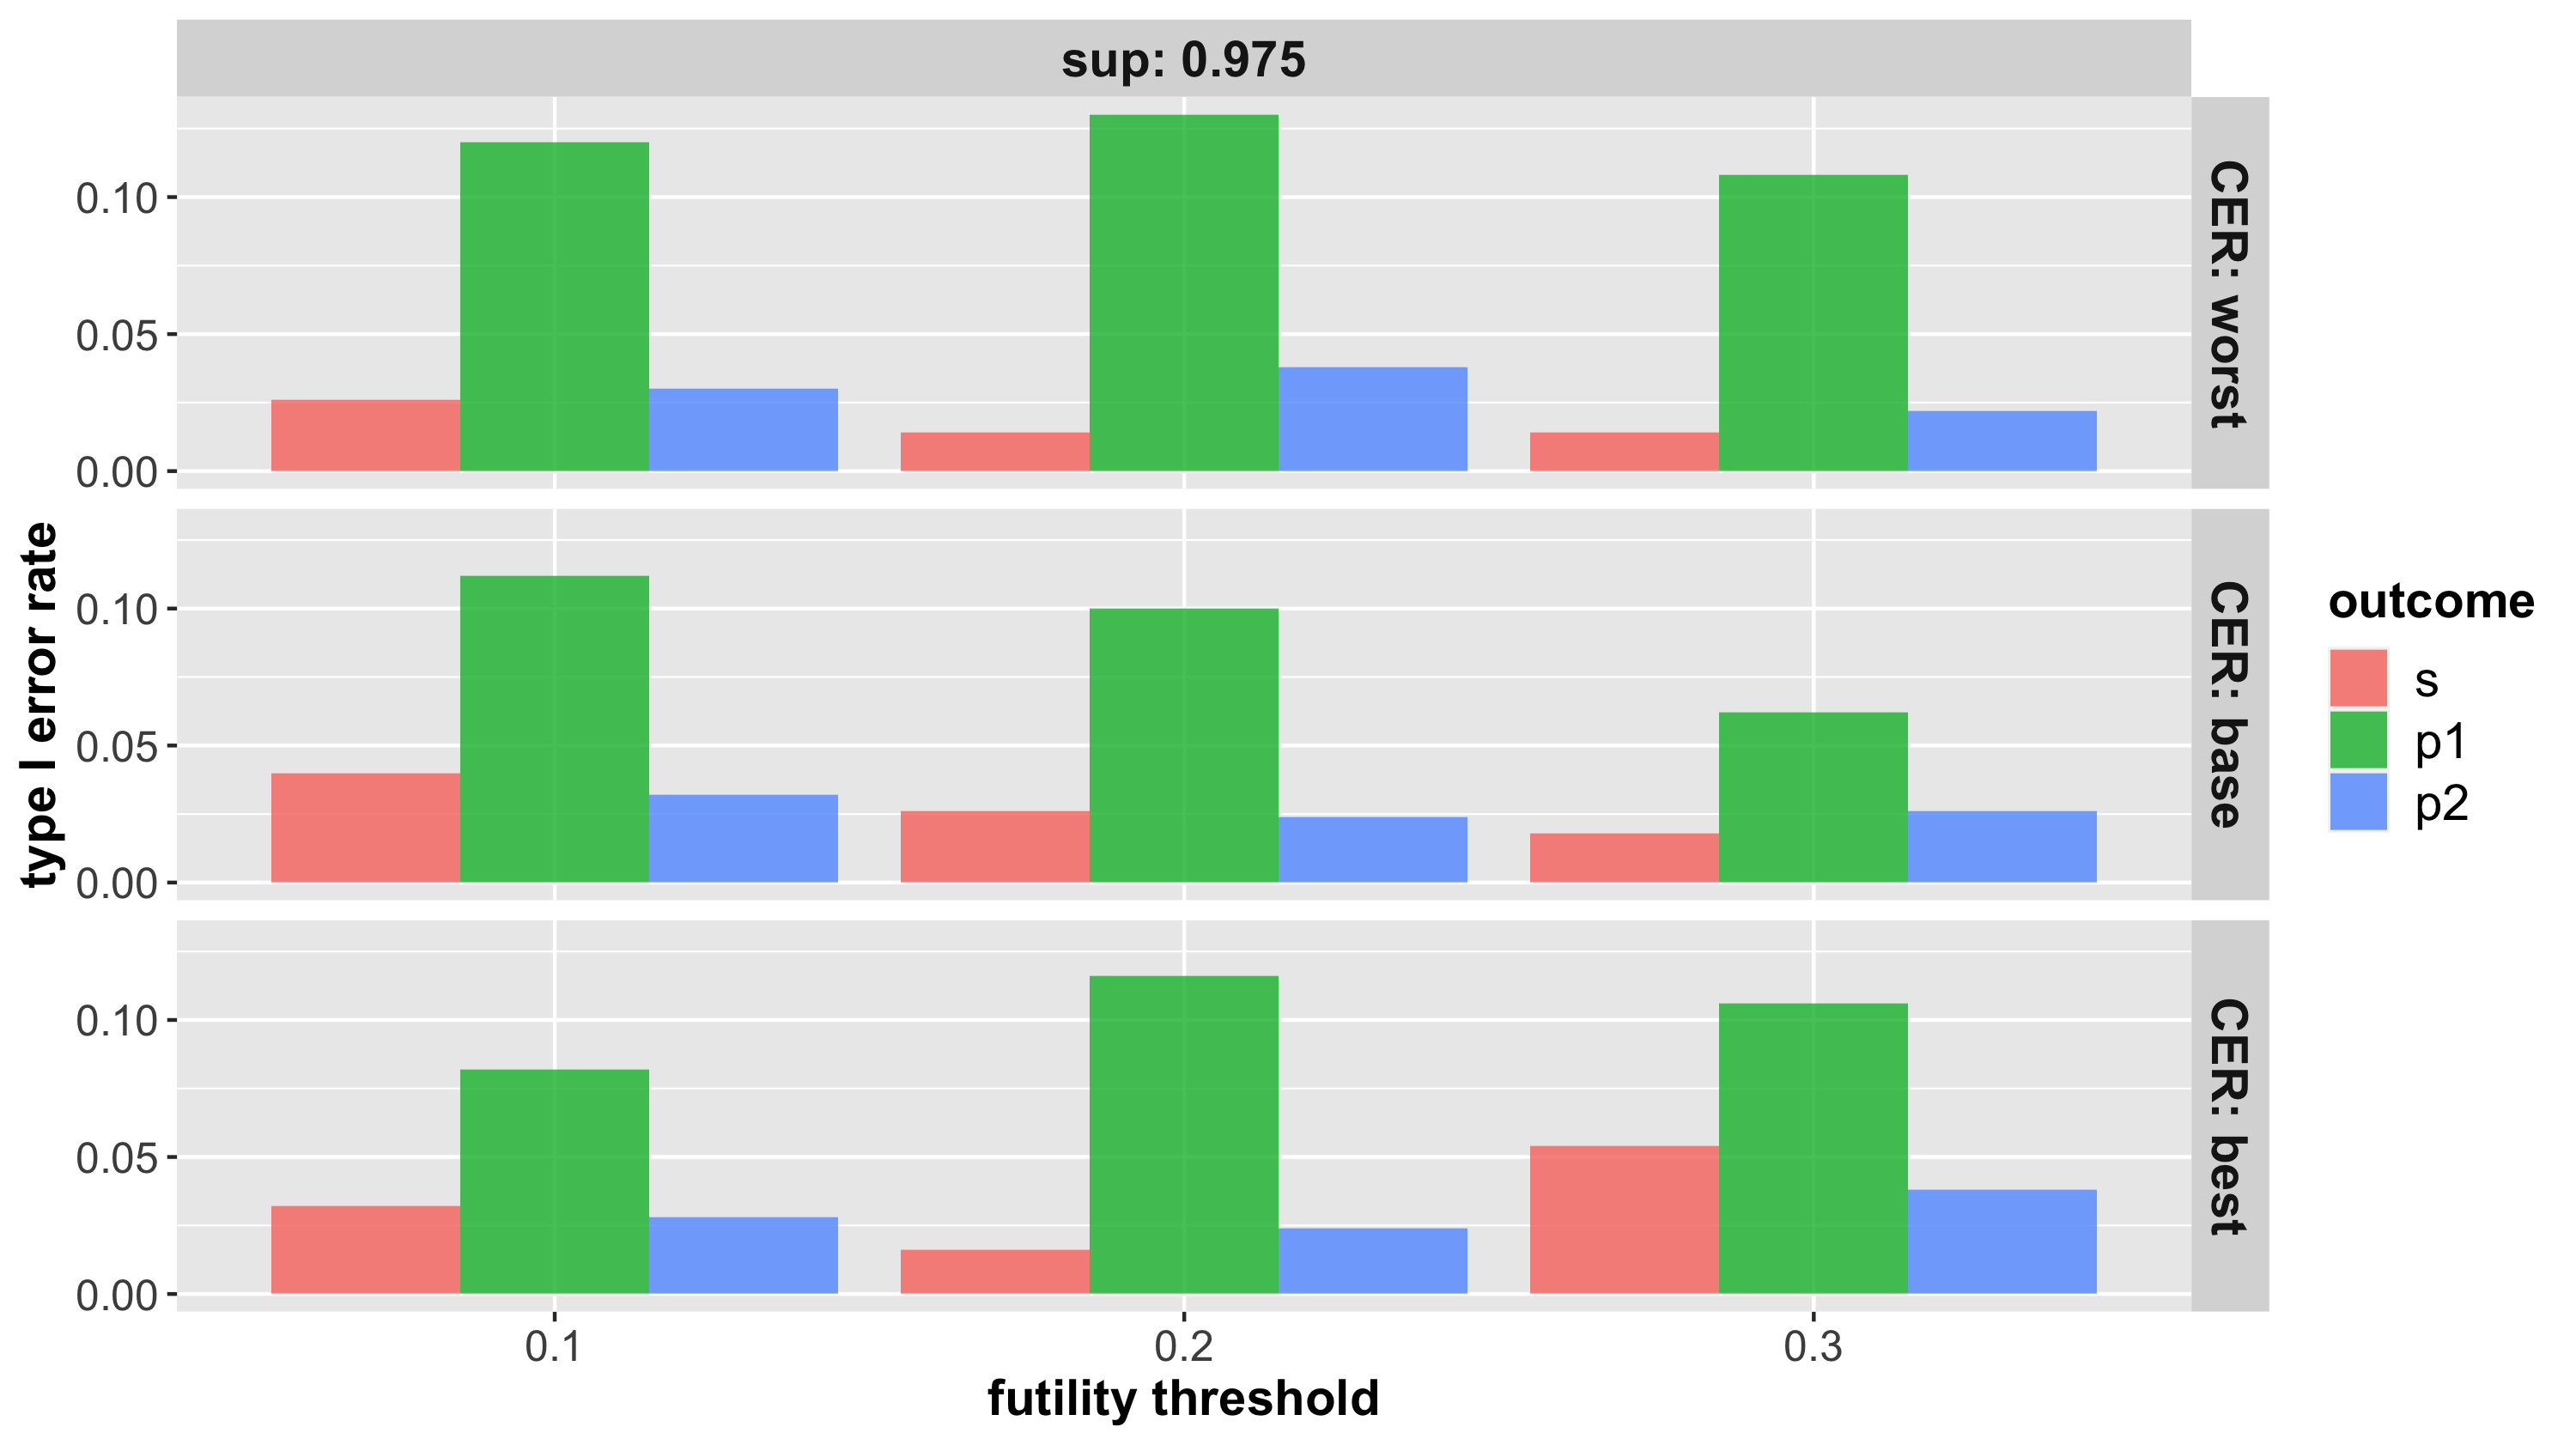
\includegraphics{../p1_plots/batch_size_nb_1000/type_1_error_p1.png}
\end{figure}

\hypertarget{power}{%
\subparagraph{Power}\label{power}}

Figure 2 displays the power for each of the outcomes under each of the
simulated scenarios and employed stopping rules. Generally, the power to
detect an effect is high for outcome p2 in all scenarios (except RRR =
0.1). The power to detect an effect for outcome p1 is high in all
scenarios where RRR=40\% or 60\%, but moderate to low when RRR is less
than 20\%. The power to detect an effect on outcome s is low in all
cases, but achieves its highest estimates when RRR=60\% and CER best
case scenario.

\begin{figure}
  \caption{Power under the three relative risk reductions (RRR - upper column label) for each of the outcomes (lower column labels). 
  Power estimates by control event rates are presented by the rows. Power estimates by the futility thresholds are presented by the bar color (see legend).}
  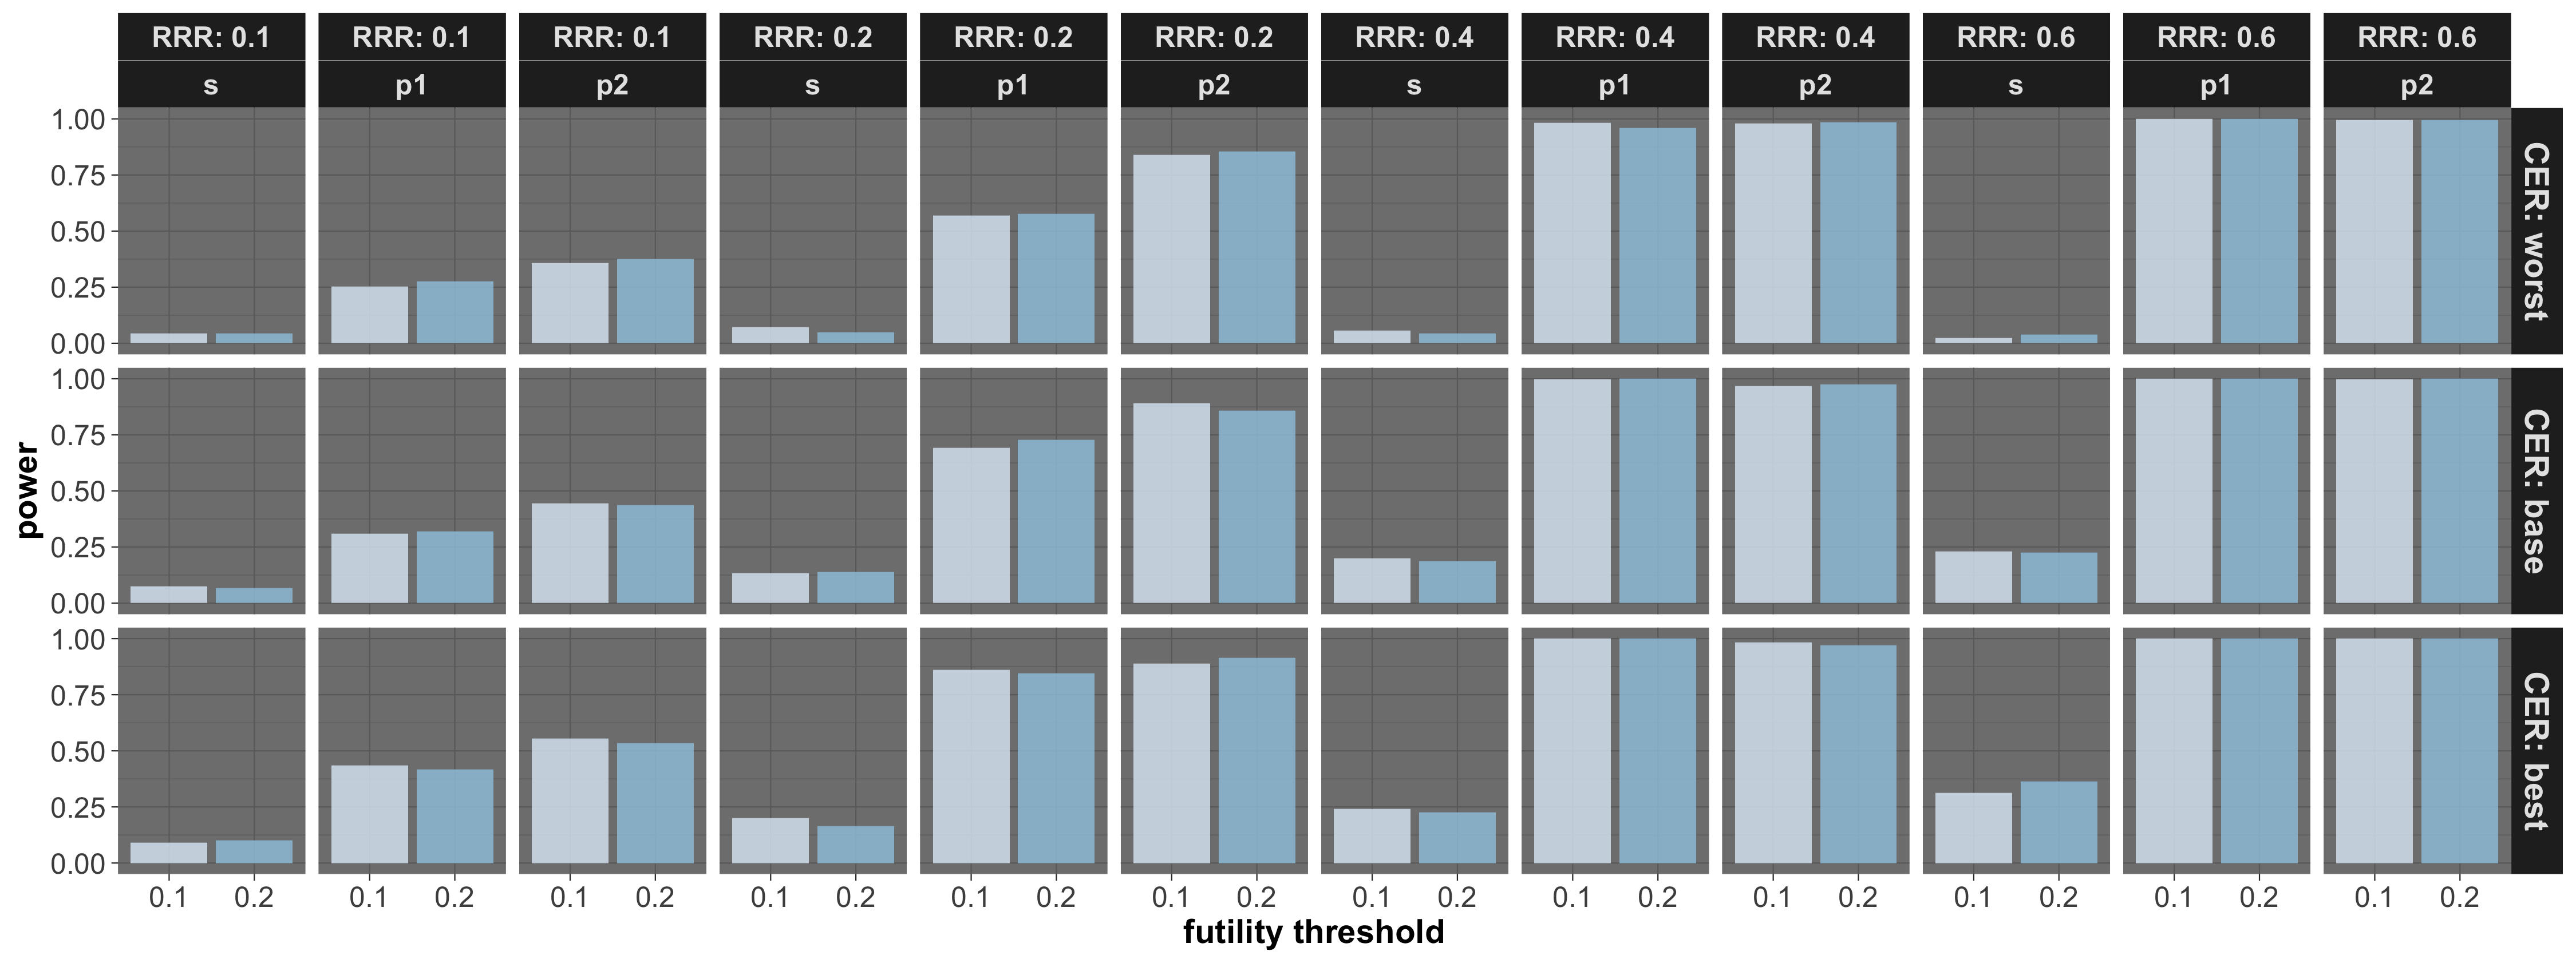
\includegraphics{../p1_plots/batch_size_nb_1000/power_all_p1.png}
\end{figure}

Figure 3. Under the true RRR=40\% and 60\%, power for outcomes p1 and p2
is very high but decreases to as the RRR becomes less than 20\%. Power
for outcome s is low for all scenarios, reaching roughly 25\% for a true
RRR=60\% and the best case CER.

\begin{figure}
  \caption{Power under the three relative risk reductions (RRR - upper column label) for each of the outcomes (lower
  column labels or legend). Observed power for each outcome is presented by colored bars. Power estimates by control
  event rates are presented by the rows and correspond to a superiority threshold of 0.975.}
  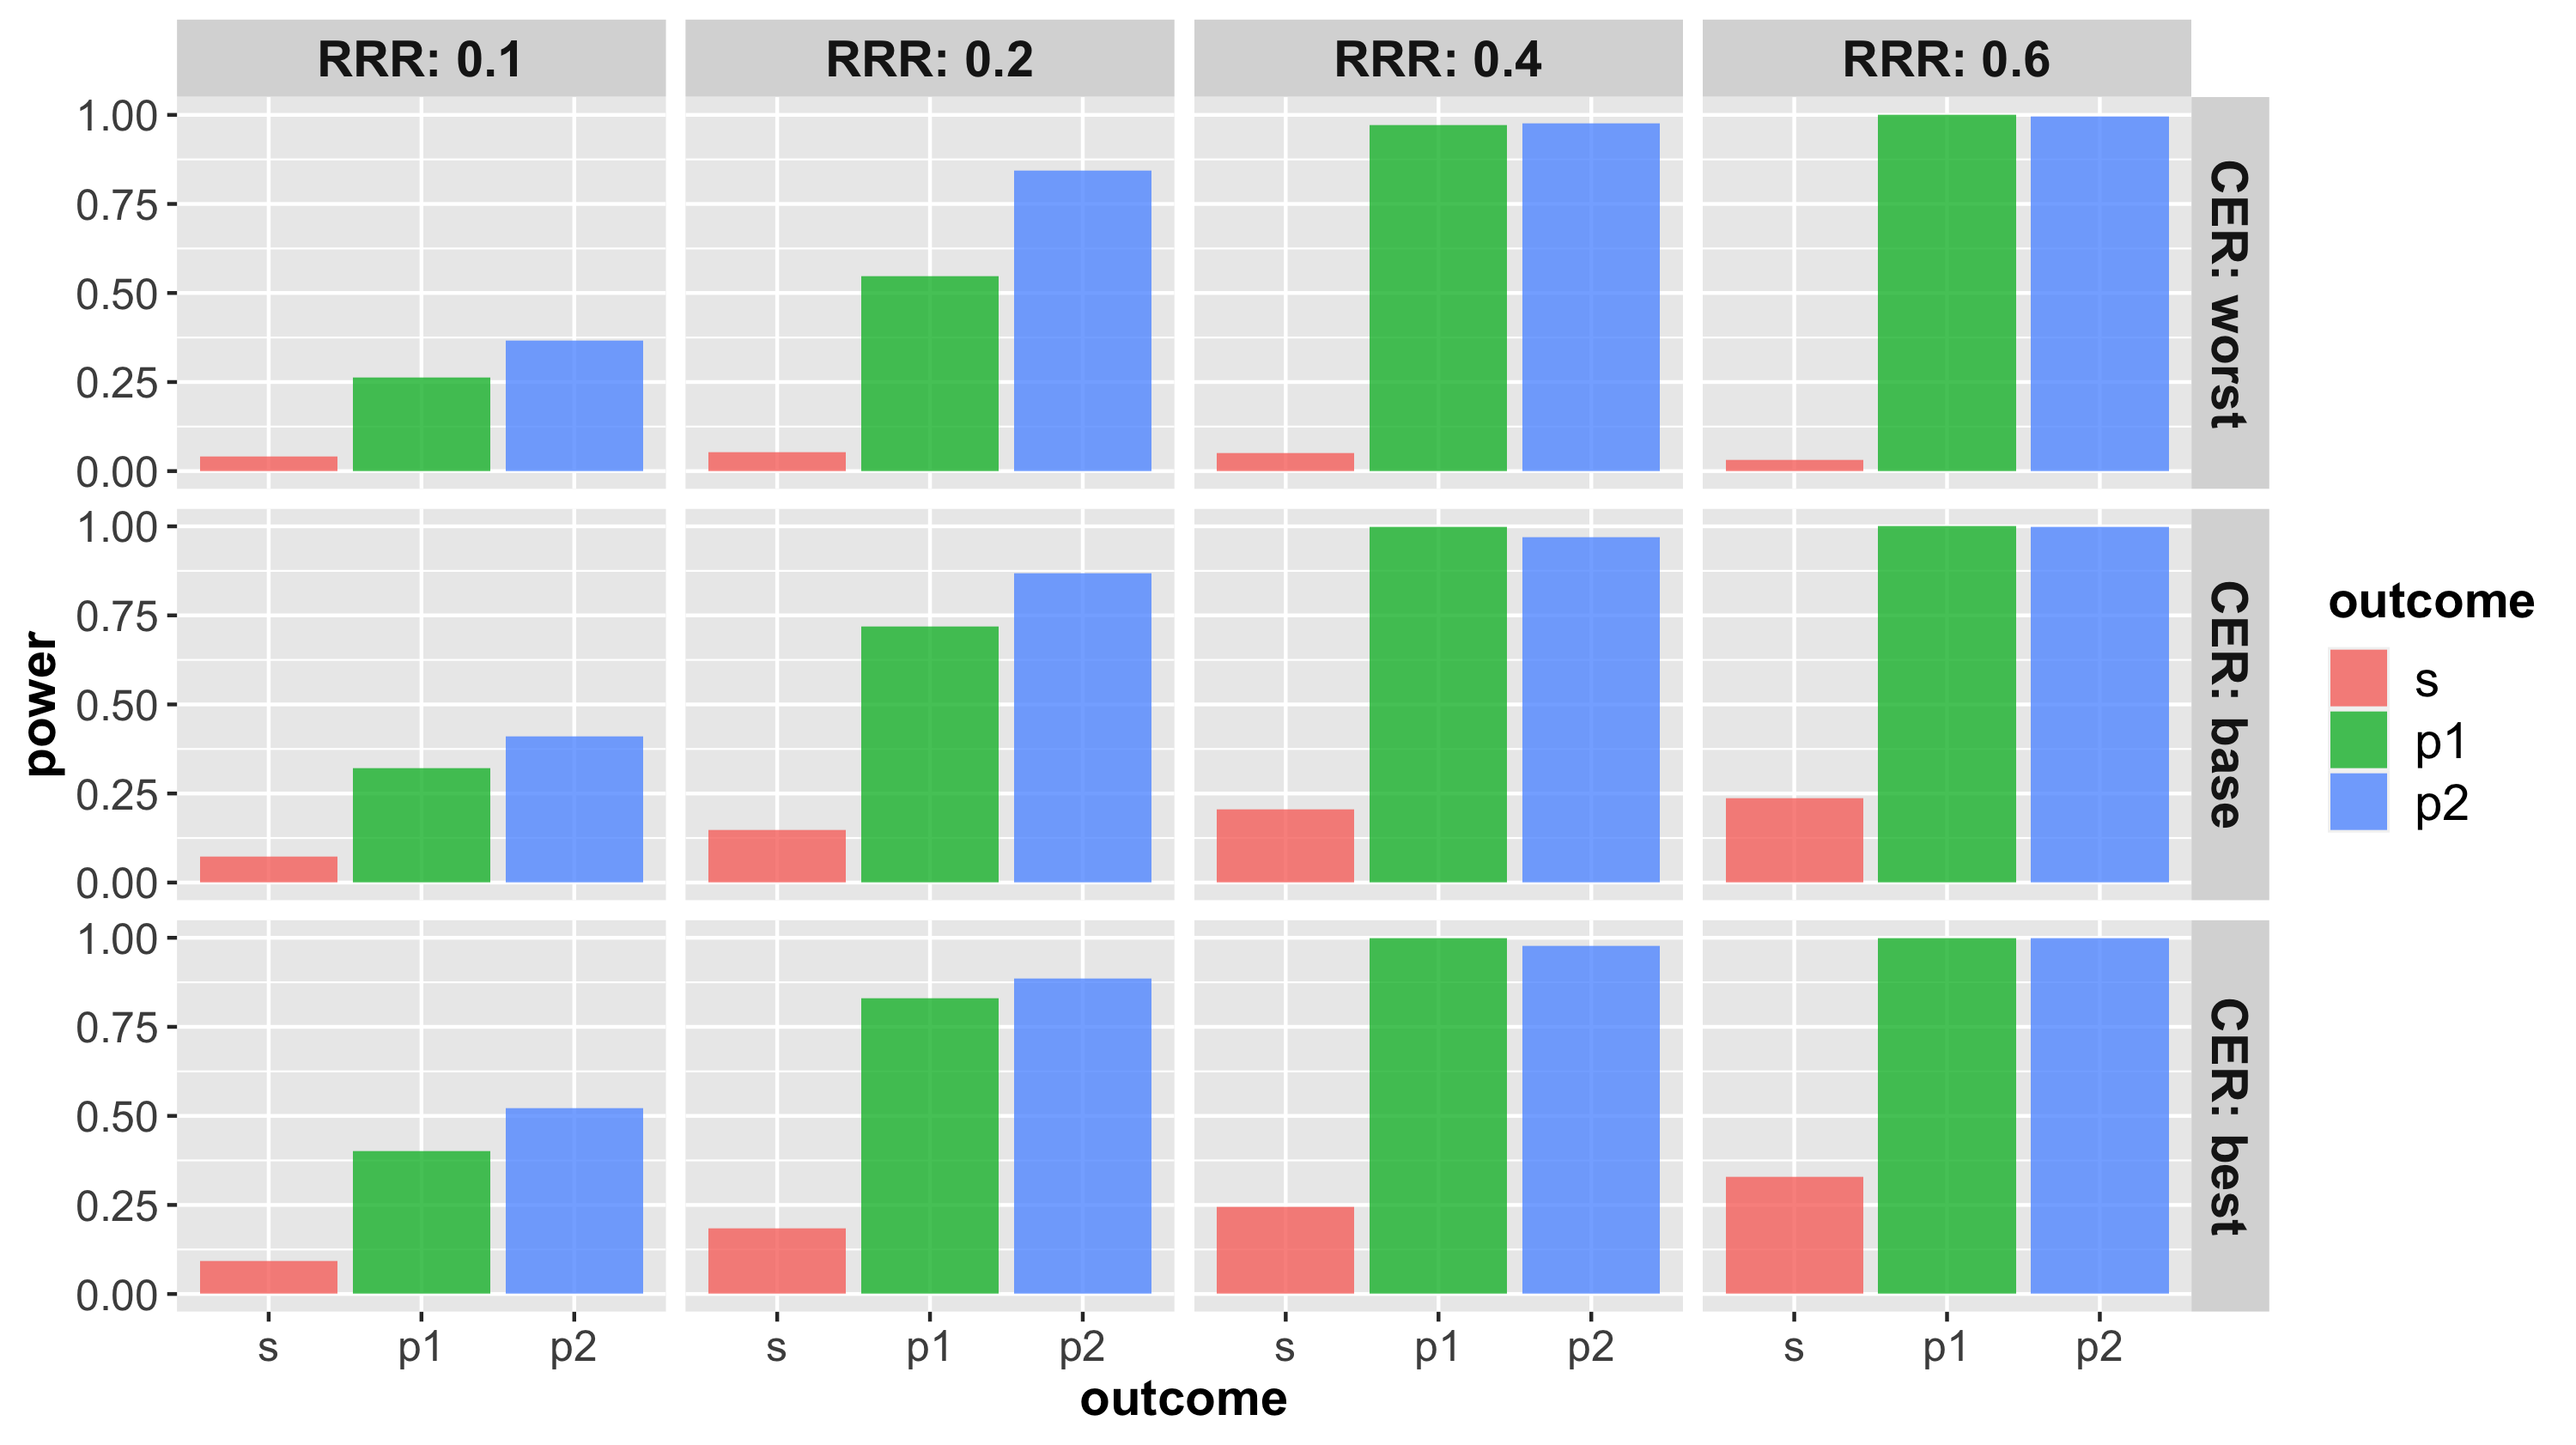
\includegraphics{../p1_plots/batch_size_nb_1000/power_p1.png}
\end{figure}

\hypertarget{expected-sample-size}{%
\subparagraph{Expected Sample Size}\label{expected-sample-size}}

Figure 4 presents the expected (mean) sample size at trial termination.
For true RRR=0, 10\% and 20\%, expected sample sizes were consistently
high, albeit with some notable reductions associated with use of a
RRR=40\% futility stopping threshold. For true of RRR=40\% and RRR=60\%,
expected sample sizes were lower and decreased as the CER improved
(worst to best).

\begin{figure}
  \caption{Expected sample size at trial termination. Results by control event scenarios are presented by rows. Results
  by relative risk reductions are presented by columns. Results by futility thresholds are presented by the color of the bars (see legend).}
  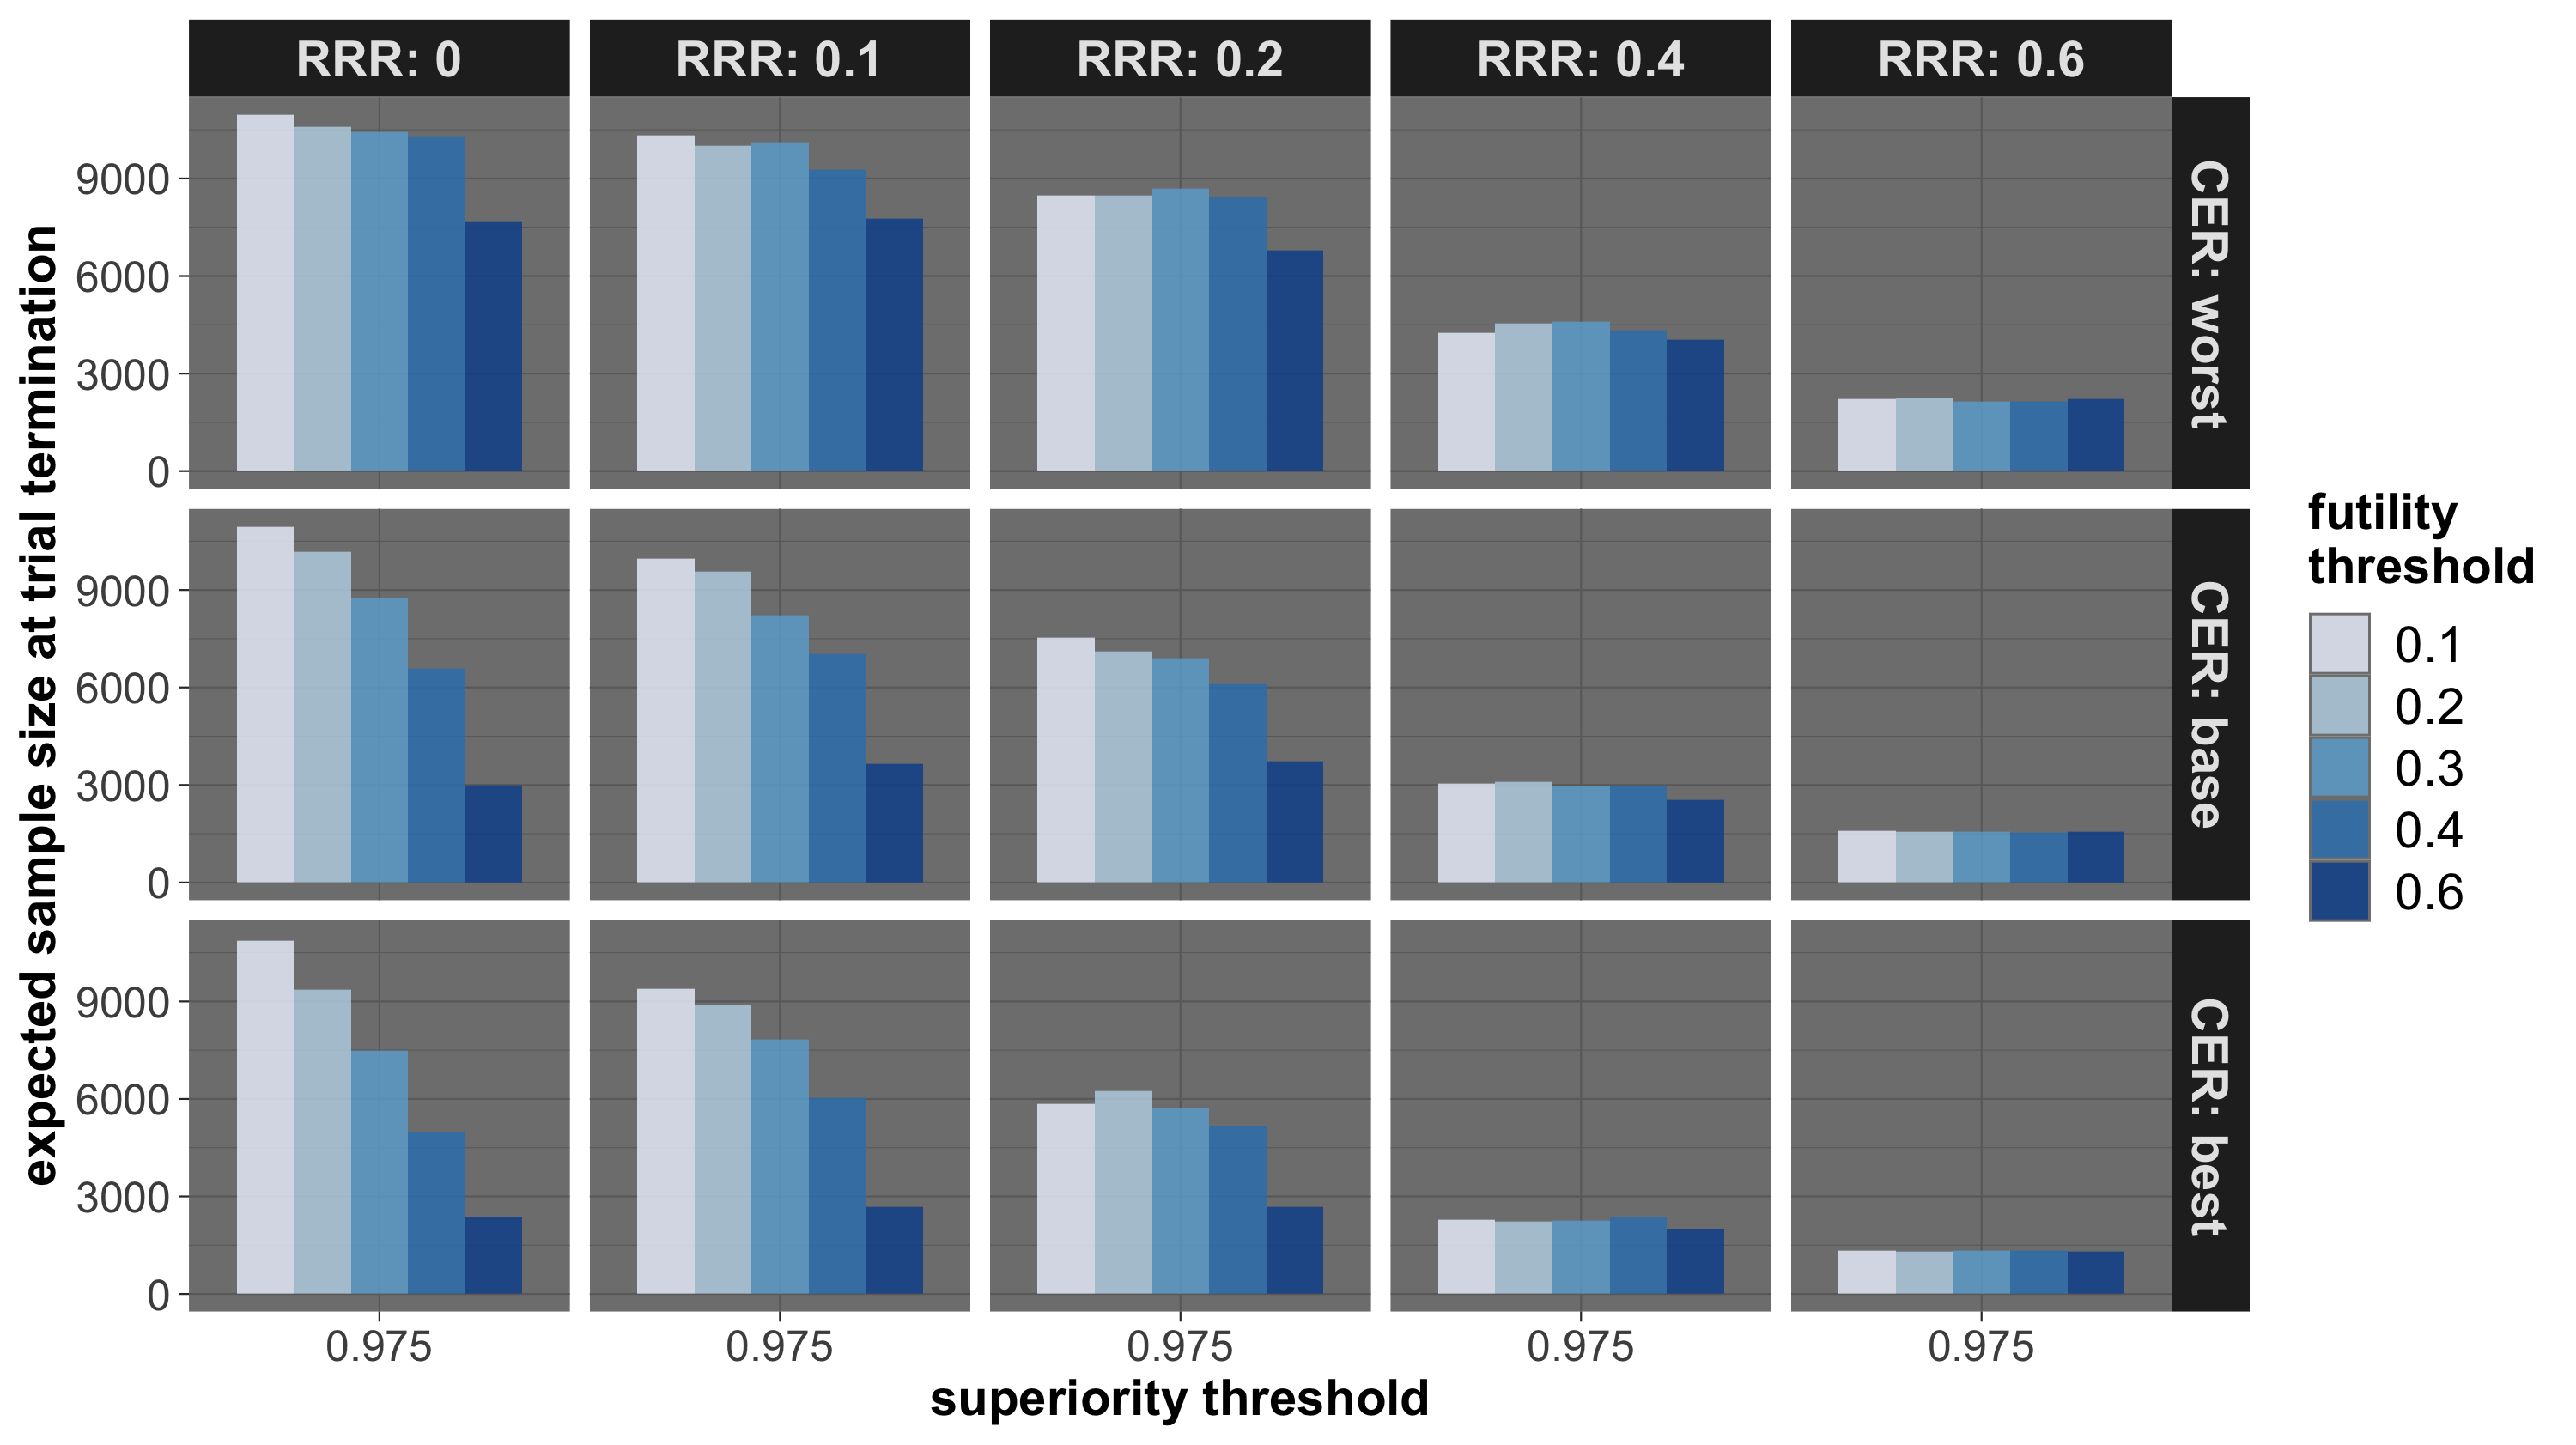
\includegraphics{../p1_plots/batch_size_nb_1000/exp_sample_size_p1.png}
\end{figure}

\hypertarget{probability-of-reaching-maximum-sample-size}{%
\paragraph{Probability of Reaching Maximum Sample
Size}\label{probability-of-reaching-maximum-sample-size}}

Figure 5 shows the probability of reaching the maximum allowed sample
size of the trial. This probability was moderate to high for the true
RRR=0, 10\% and 20\%, and generally decreased as the CER improved. For
RRR=40\% and RRR=60\%, this probability was negligible for all cases.

\begin{figure}
  \caption{Probability of reaching maximum sample size for the three control event rates (CER – rows), four relative
  risk reductions (RRR – columns), and three futility thresholds (legend).}
  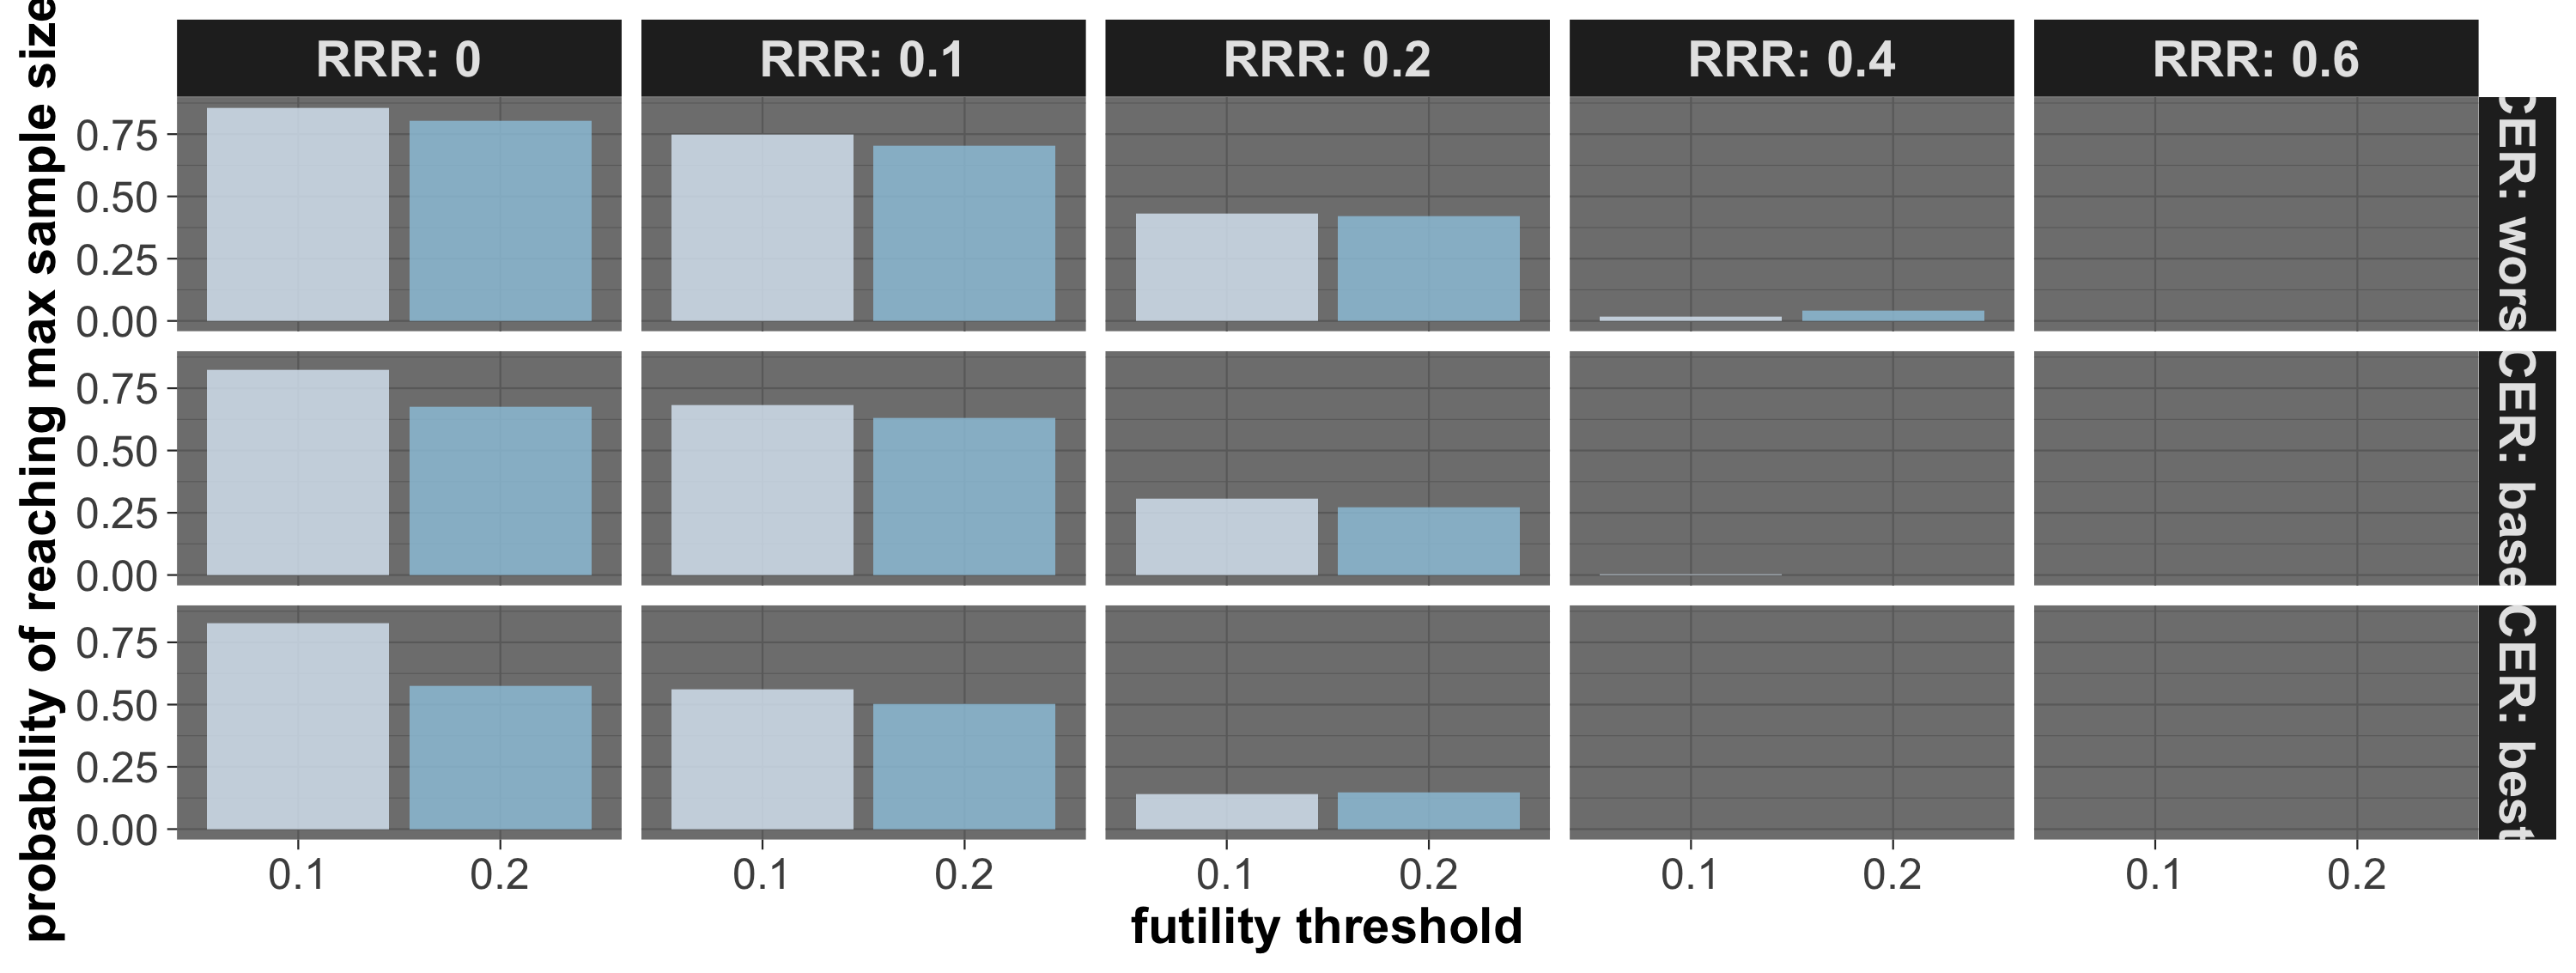
\includegraphics{../p1_plots/batch_size_nb_1000/prob_reach_max_size_p1.png}
\end{figure}

\hypertarget{probability-of-stopping-early}{%
\paragraph{Probability of Stopping
Early}\label{probability-of-stopping-early}}

The probability of stopping early was obtained overall, for superiority
and for futility. Figure 6 displays the overall probability of stopping
early, Figure 7(a) displays the probability of stopping early for
futility and figure 7(b) displays the probability of stopping early for
superiority. The overall probability of stopping early is strongly
positively correlated with the CER and RRR. When the simulated RRR=0\%,
10\% and 20\%, the overall probability of stopping early is also highly
correlated to the futility threshold.

\begin{figure}
  \caption{Probability of stopping early due to futility or superiority for the three control event rates (CER – rows),
  four relative risk reductions (RRR – columns), three superiority thresholds (x axis) and three futility thresholds
  (legend).}
  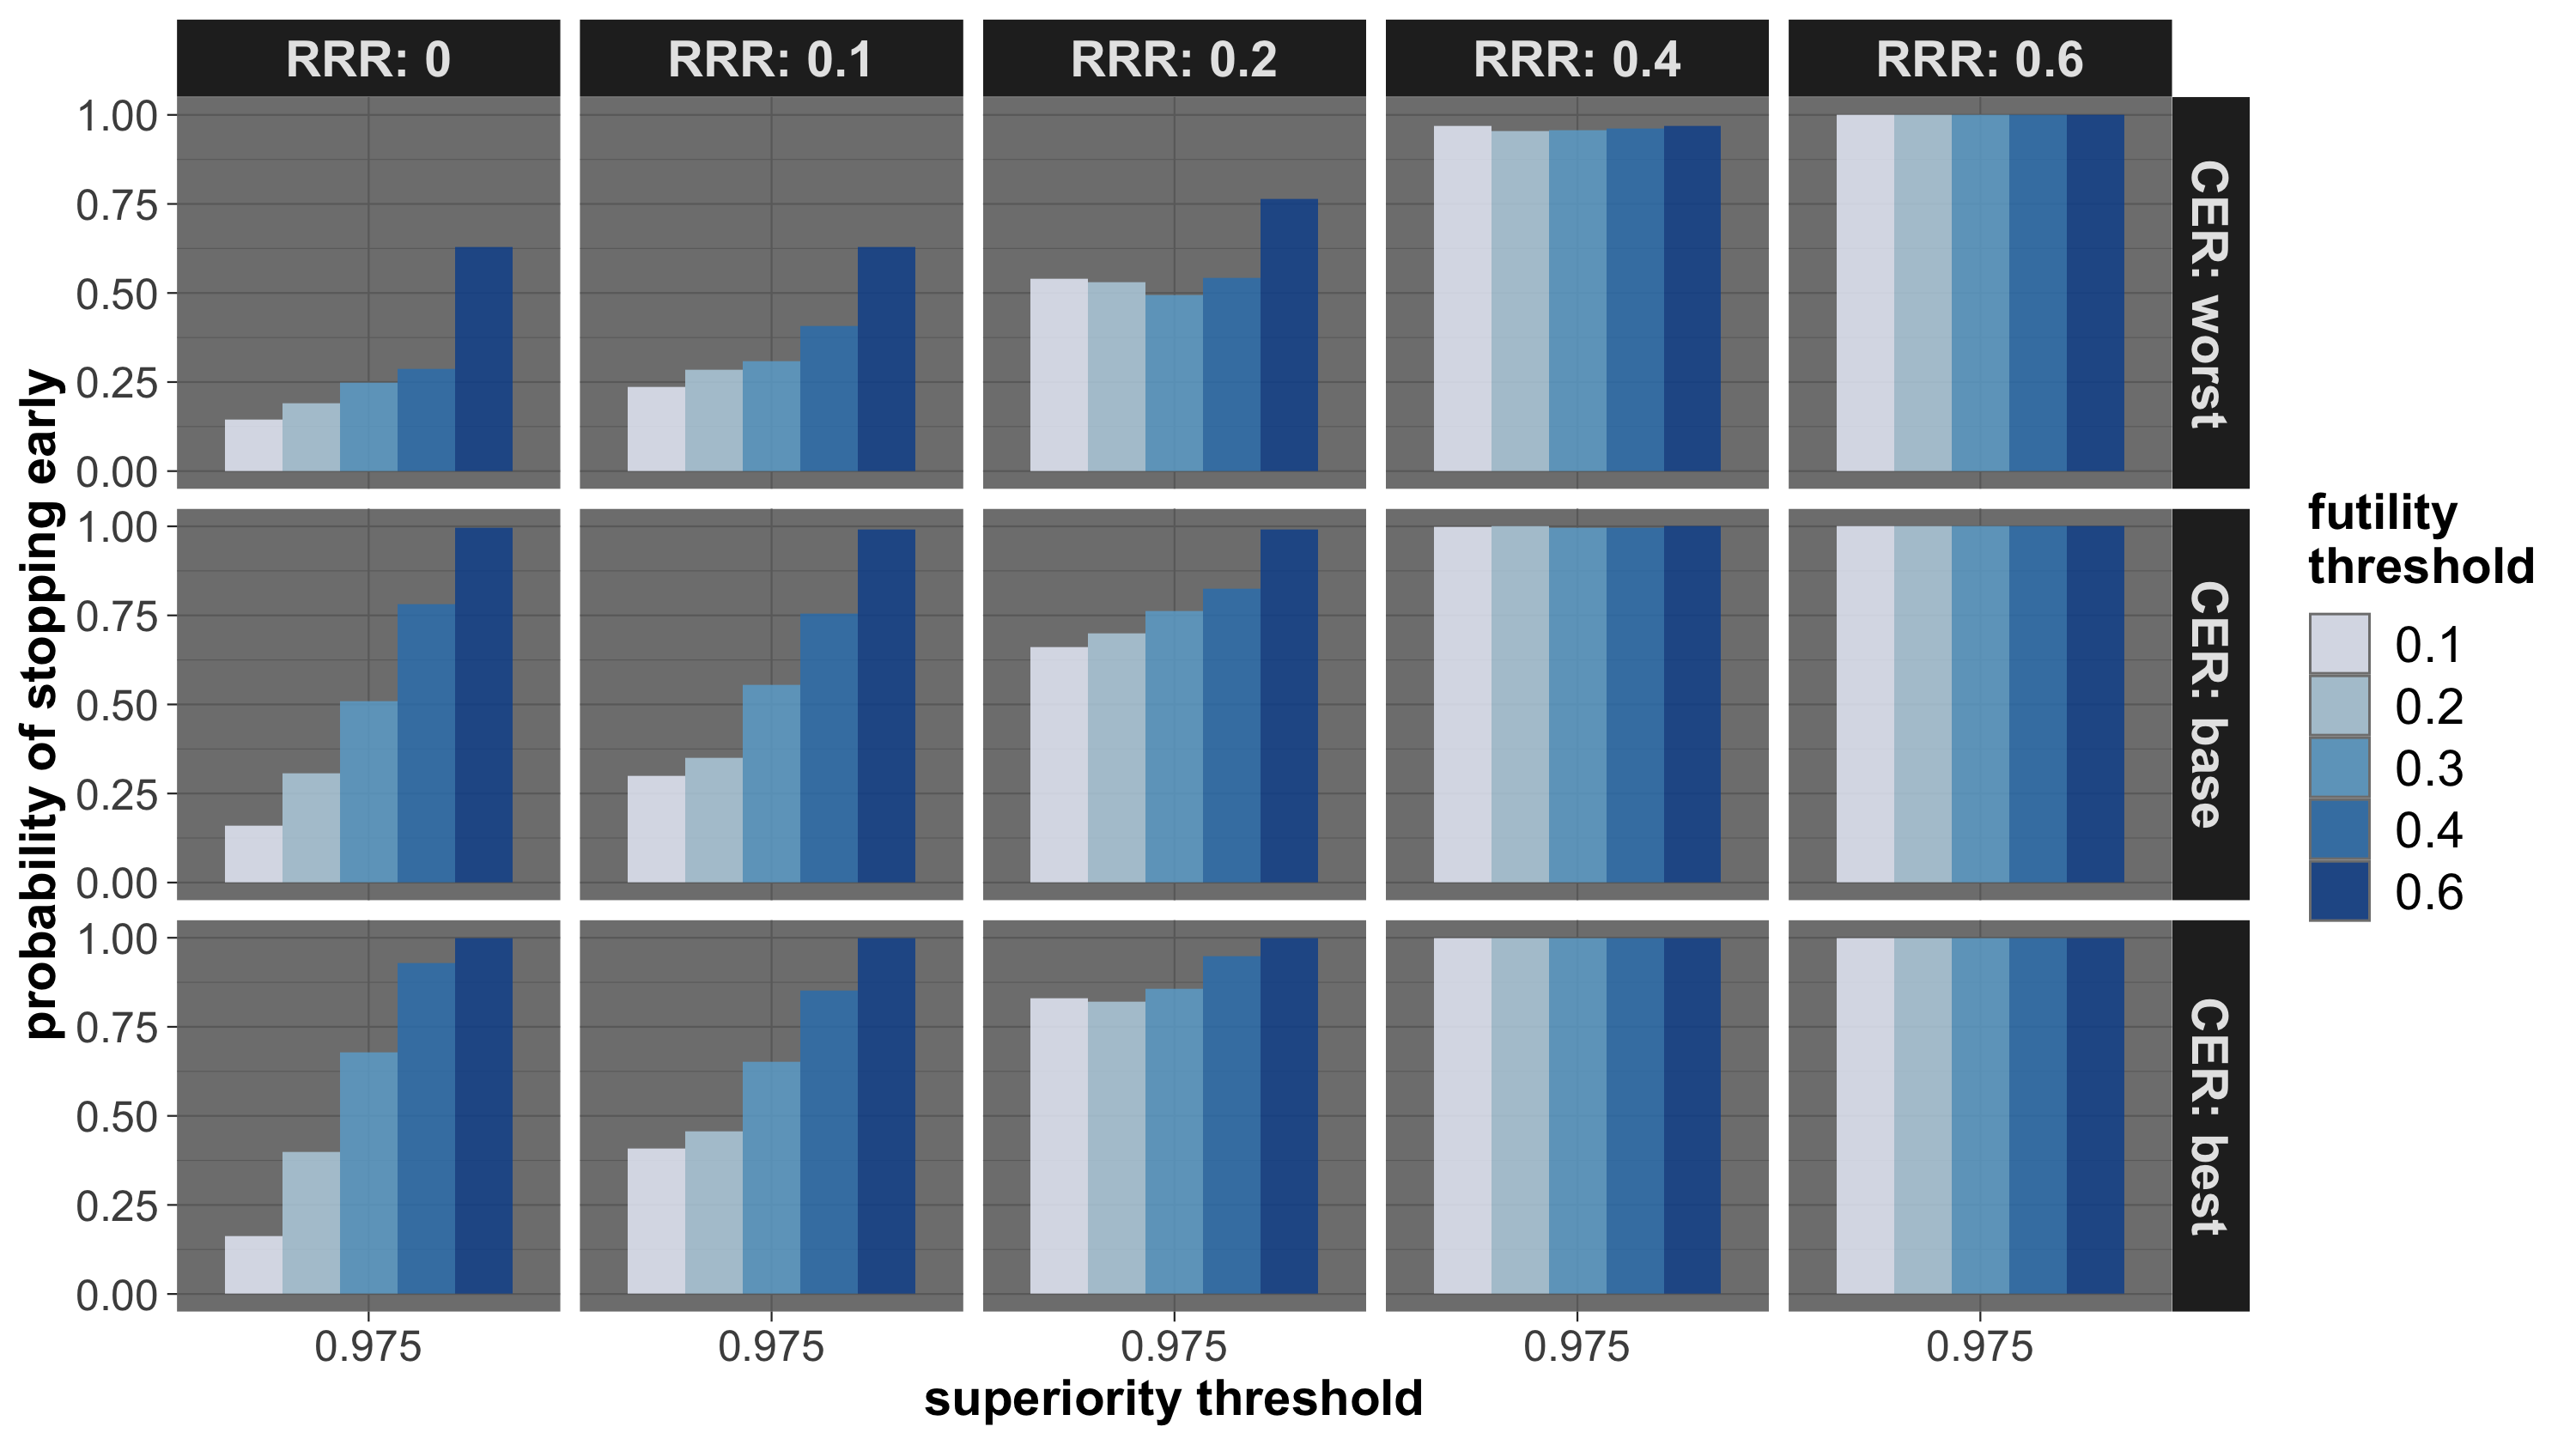
\includegraphics{../p1_plots/batch_size_nb_1000/prob_stop_early_p1.png}
\end{figure}

The RRR=40\% futility threshold results in consistently greater than
80-90\% probability of stopping early for the base and best-case CER
scenarios when true RRR=0\% (similar trend observed for expected sample
size results Figure 3). Stopping early for futility when the simulated
RRR=0\% is likely with futility thresholds of \textgreater{}30\%, but
less so with a futility threshold of 20\%. A futility threshold of
\textgreater{}40\% also results in a moderately low probability of
stopping early where the true RRR=20\%. The probability of stopping
early for superiority is close to 100\% for all CERs when the true
RRR=40\% or RRR=60\%, regardless of futility threshold. For the true
RRR=20\%, there is moderate probability of stopping early which
increases with improving CER and decreases with higher futility
thresholds. The lower probability of stopping for superiority when the
true RRR=0 explained by the high probability of stopping for futility in
this setting.

\begin{figure}
\centering
  \caption{Probability of stopping early due to futility, and stopping early due to superiority. Stopping probabilities
  are presented for the three control event rates (CER – rows), four relative risk reductions (RRR – columns), and three futility thresholds (legend).}
  \label{fig:fig}
  \begin{subfigure}{0.8\textwidth}
    \centering
    \caption{}
    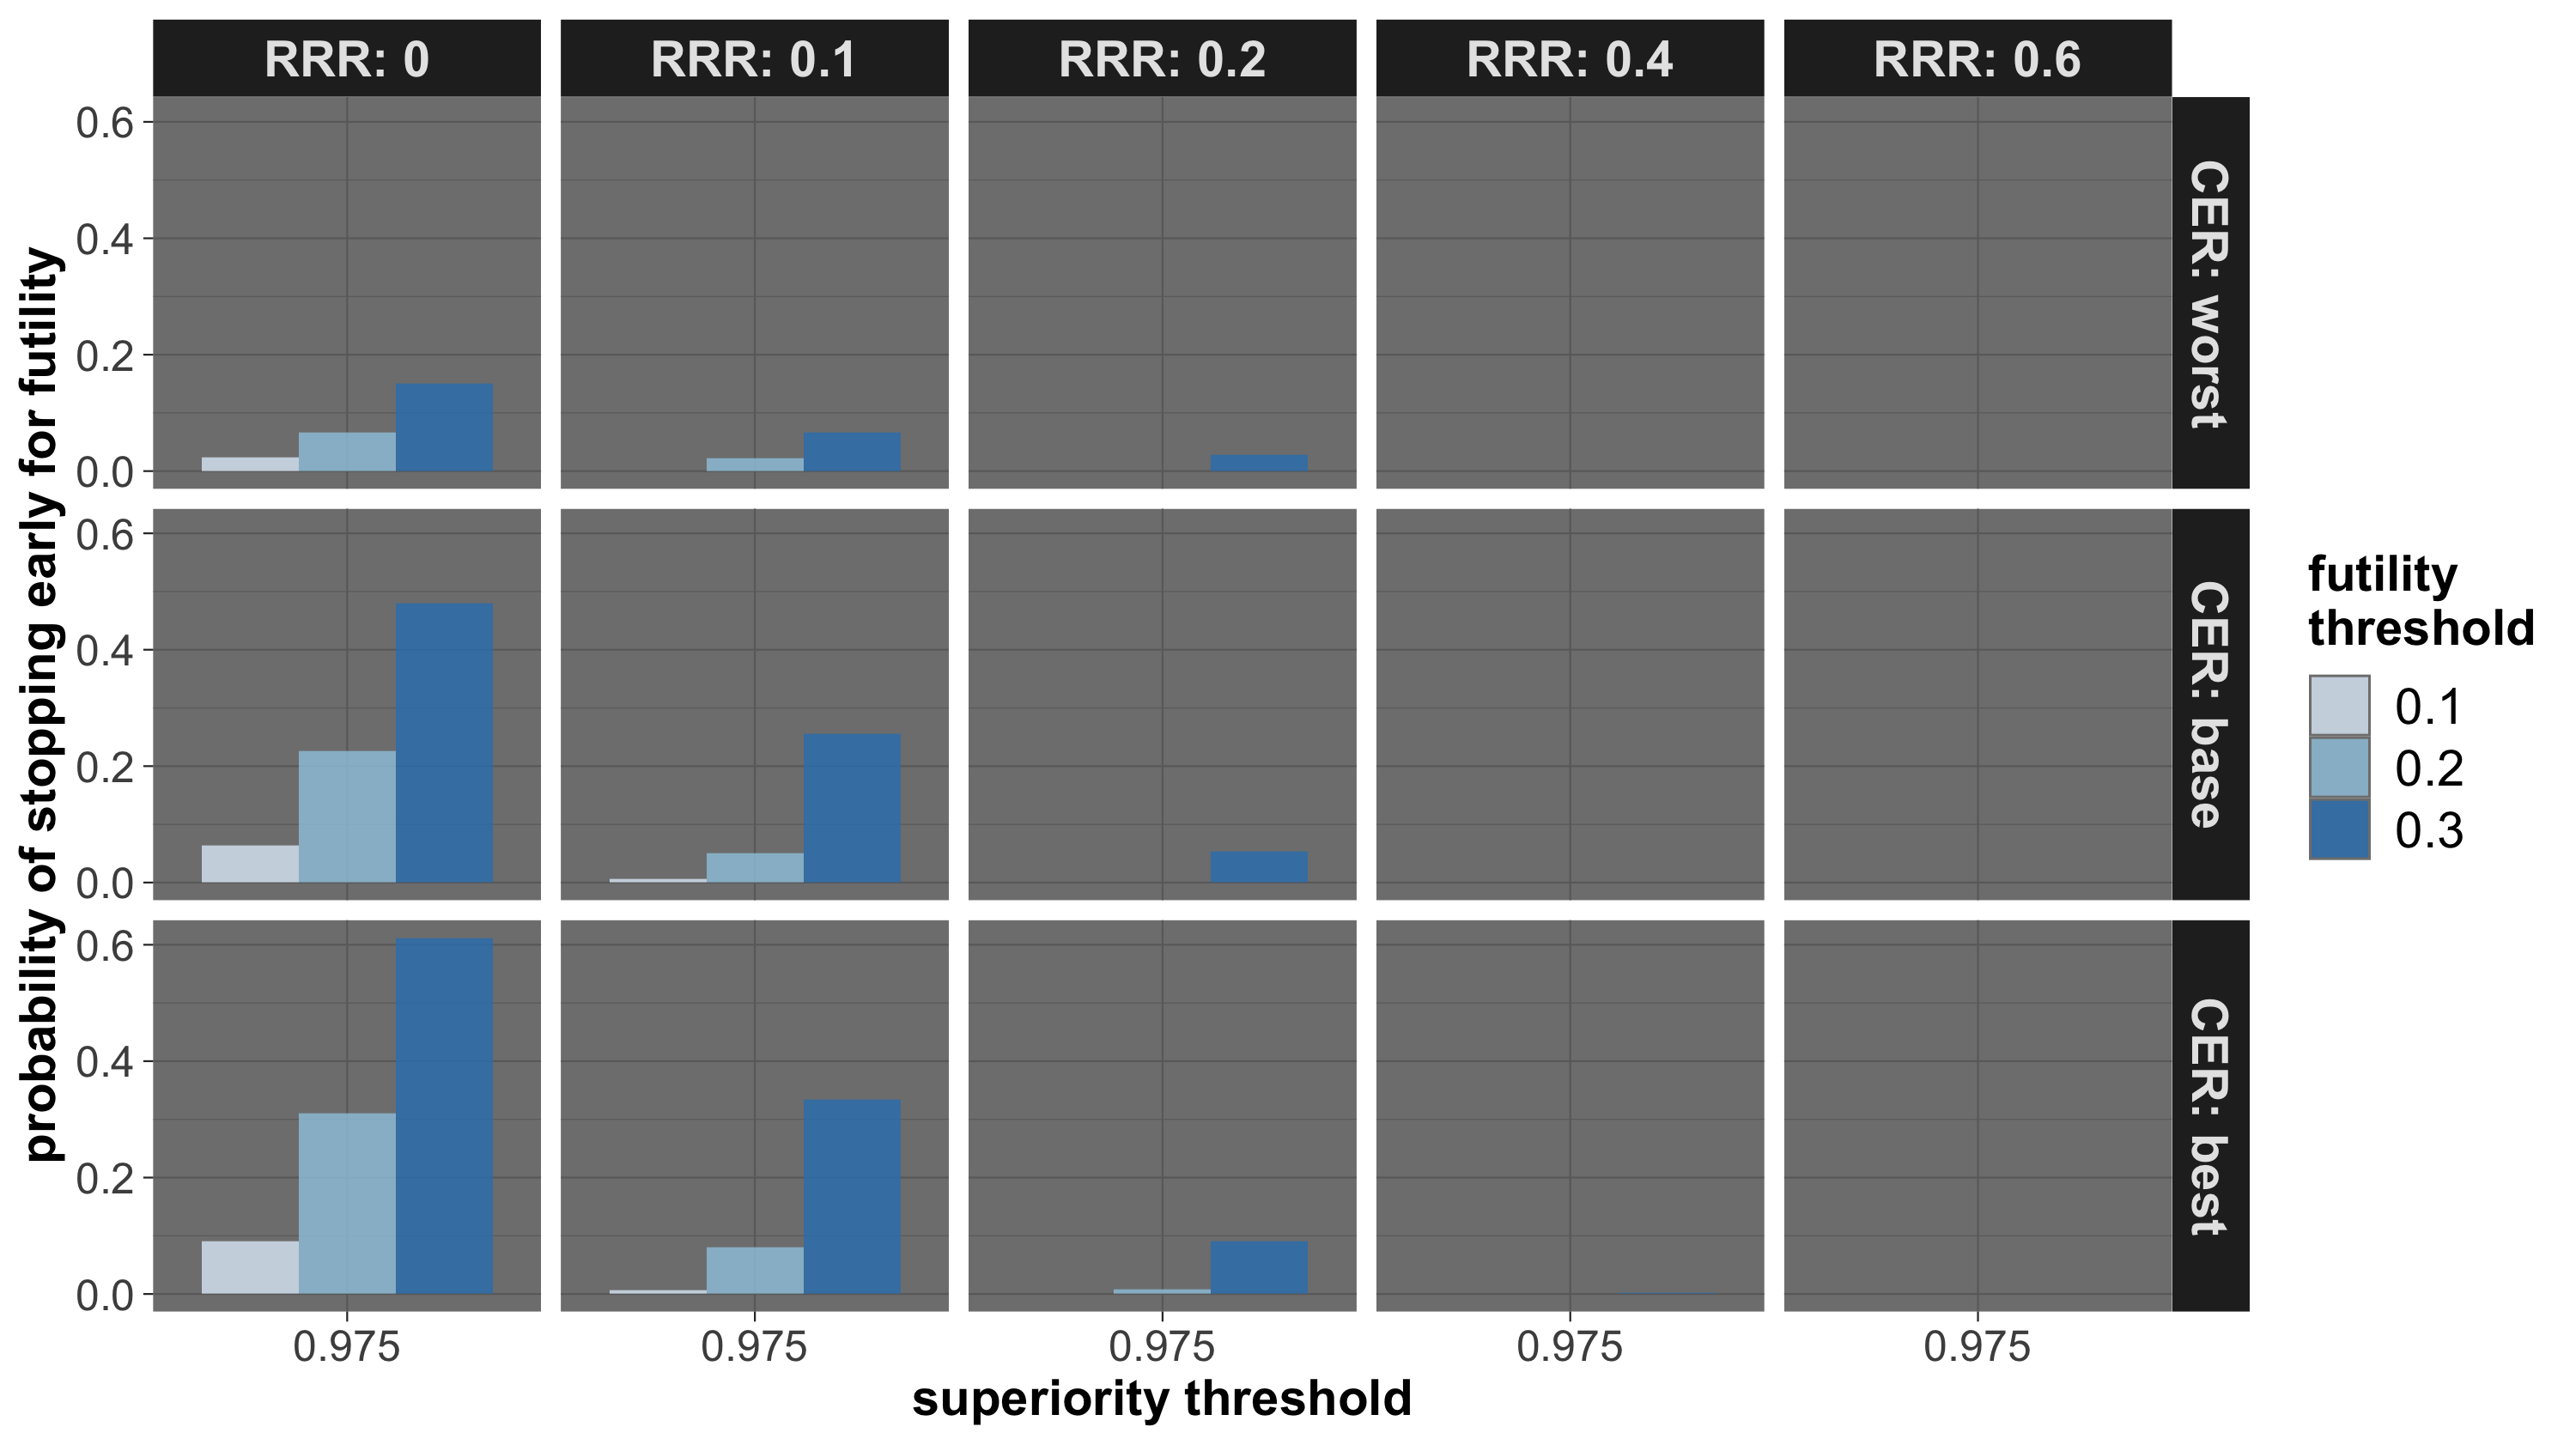
\includegraphics{../p1_plots/batch_size_nb_1000/prob_stop_early_fut_p1.png}
  \end{subfigure}
  \begin{subfigure}{0.8\textwidth}
    \centering
    \caption{}
    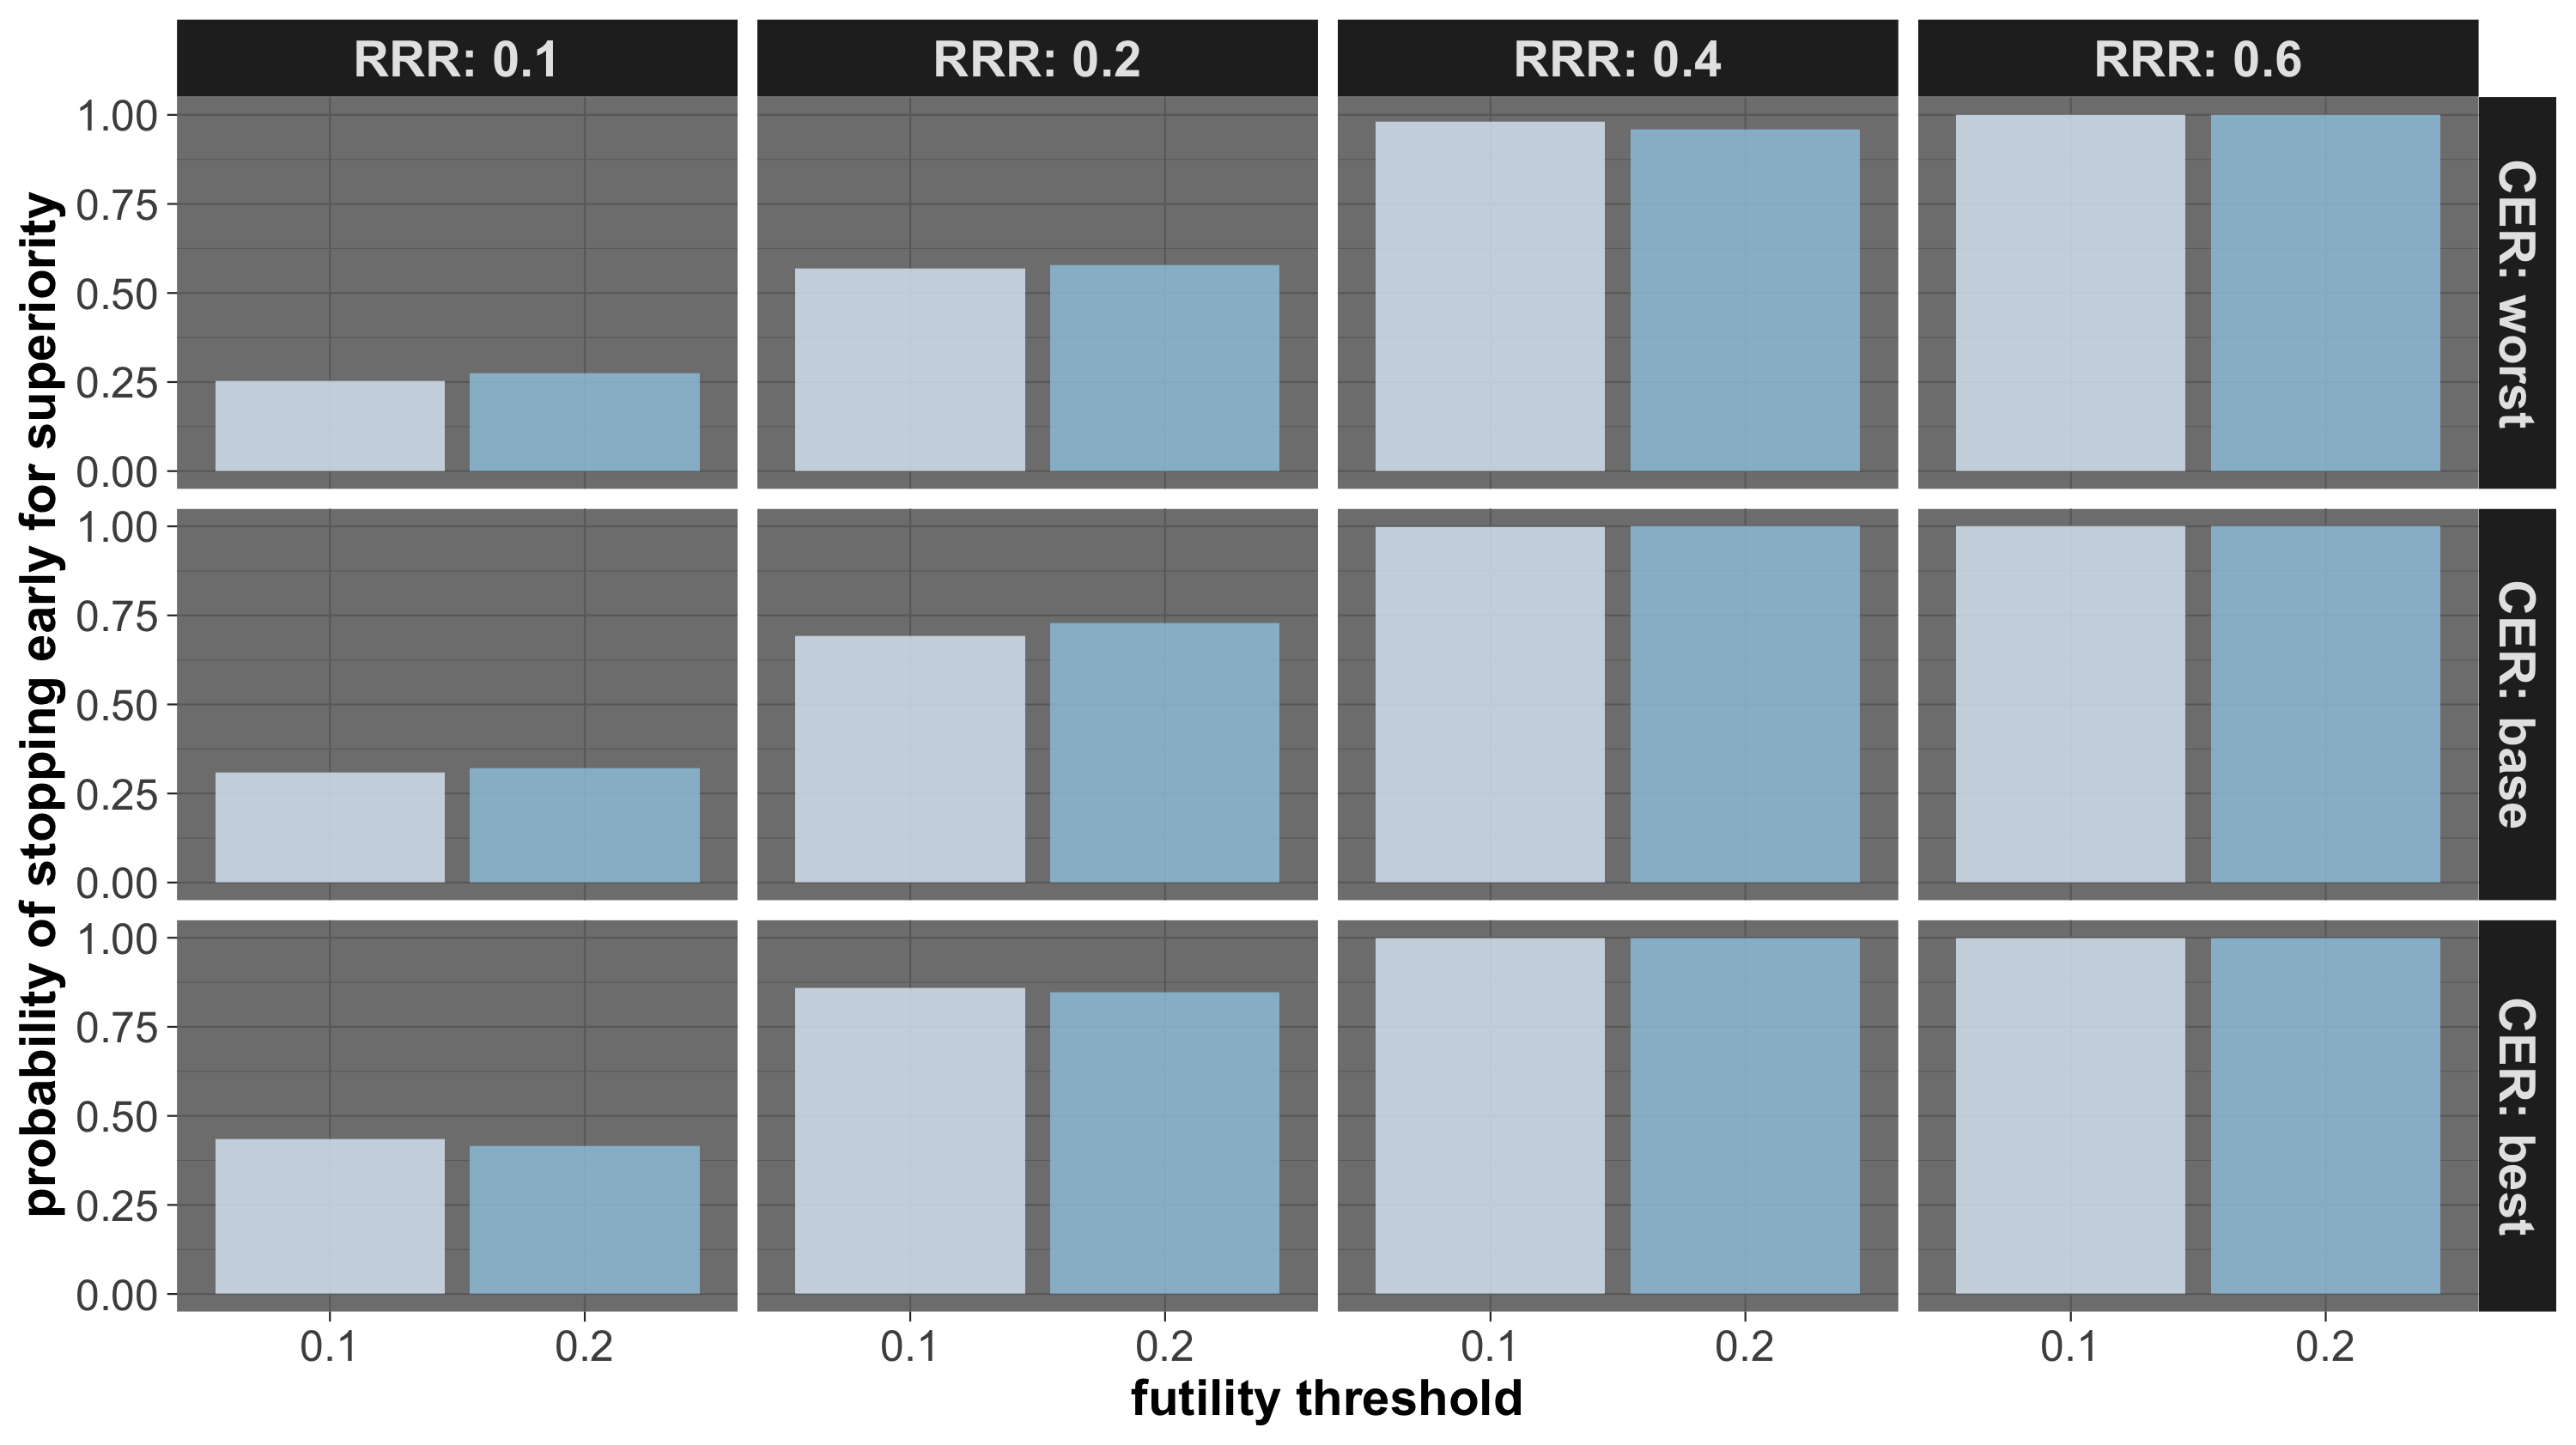
\includegraphics{../p1_plots/batch_size_nb_1000/prob_stop_early_sup_p1.png}
  \end{subfigure}
\end{figure}

\hypertarget{p-values-at-trial-termination-when-a-true-effect-exists}{%
\paragraph{P-values at trial termination when a true effect
exists}\label{p-values-at-trial-termination-when-a-true-effect-exists}}

Figure 8 presents the categorical distribution of p-values
(\textless{}5\%, 5-10\%, or \textgreater{}10\%) upon trial termination
(stopping early or reaching max. allowed sample size). Figure 9(a) and
9(b) presents the divide of p-values when stopping for futility (a) and
superiority (b), respectively.

The overall probability of observing a p-value less than 5\% (i.e., a
conventionally statistically significant difference) is high or close to
100\% in scenarios when RRR=40\% or 60\% across all CER scenarios for
outcomes p1 and p2. Outcome s has a greater proportion of p-values being
\textgreater{}10\% in these scenarios.

\begin{figure}
  \caption{Overall probability at trial termination that the p-value (from Fisher’s exact test) at termination of the
  trial is below 5\%, between 5\% and 10\% and greater than 10\%. The rows represent the three control even rate scenarios
  and the three columns present the three relative risk reduction scenarios.}
  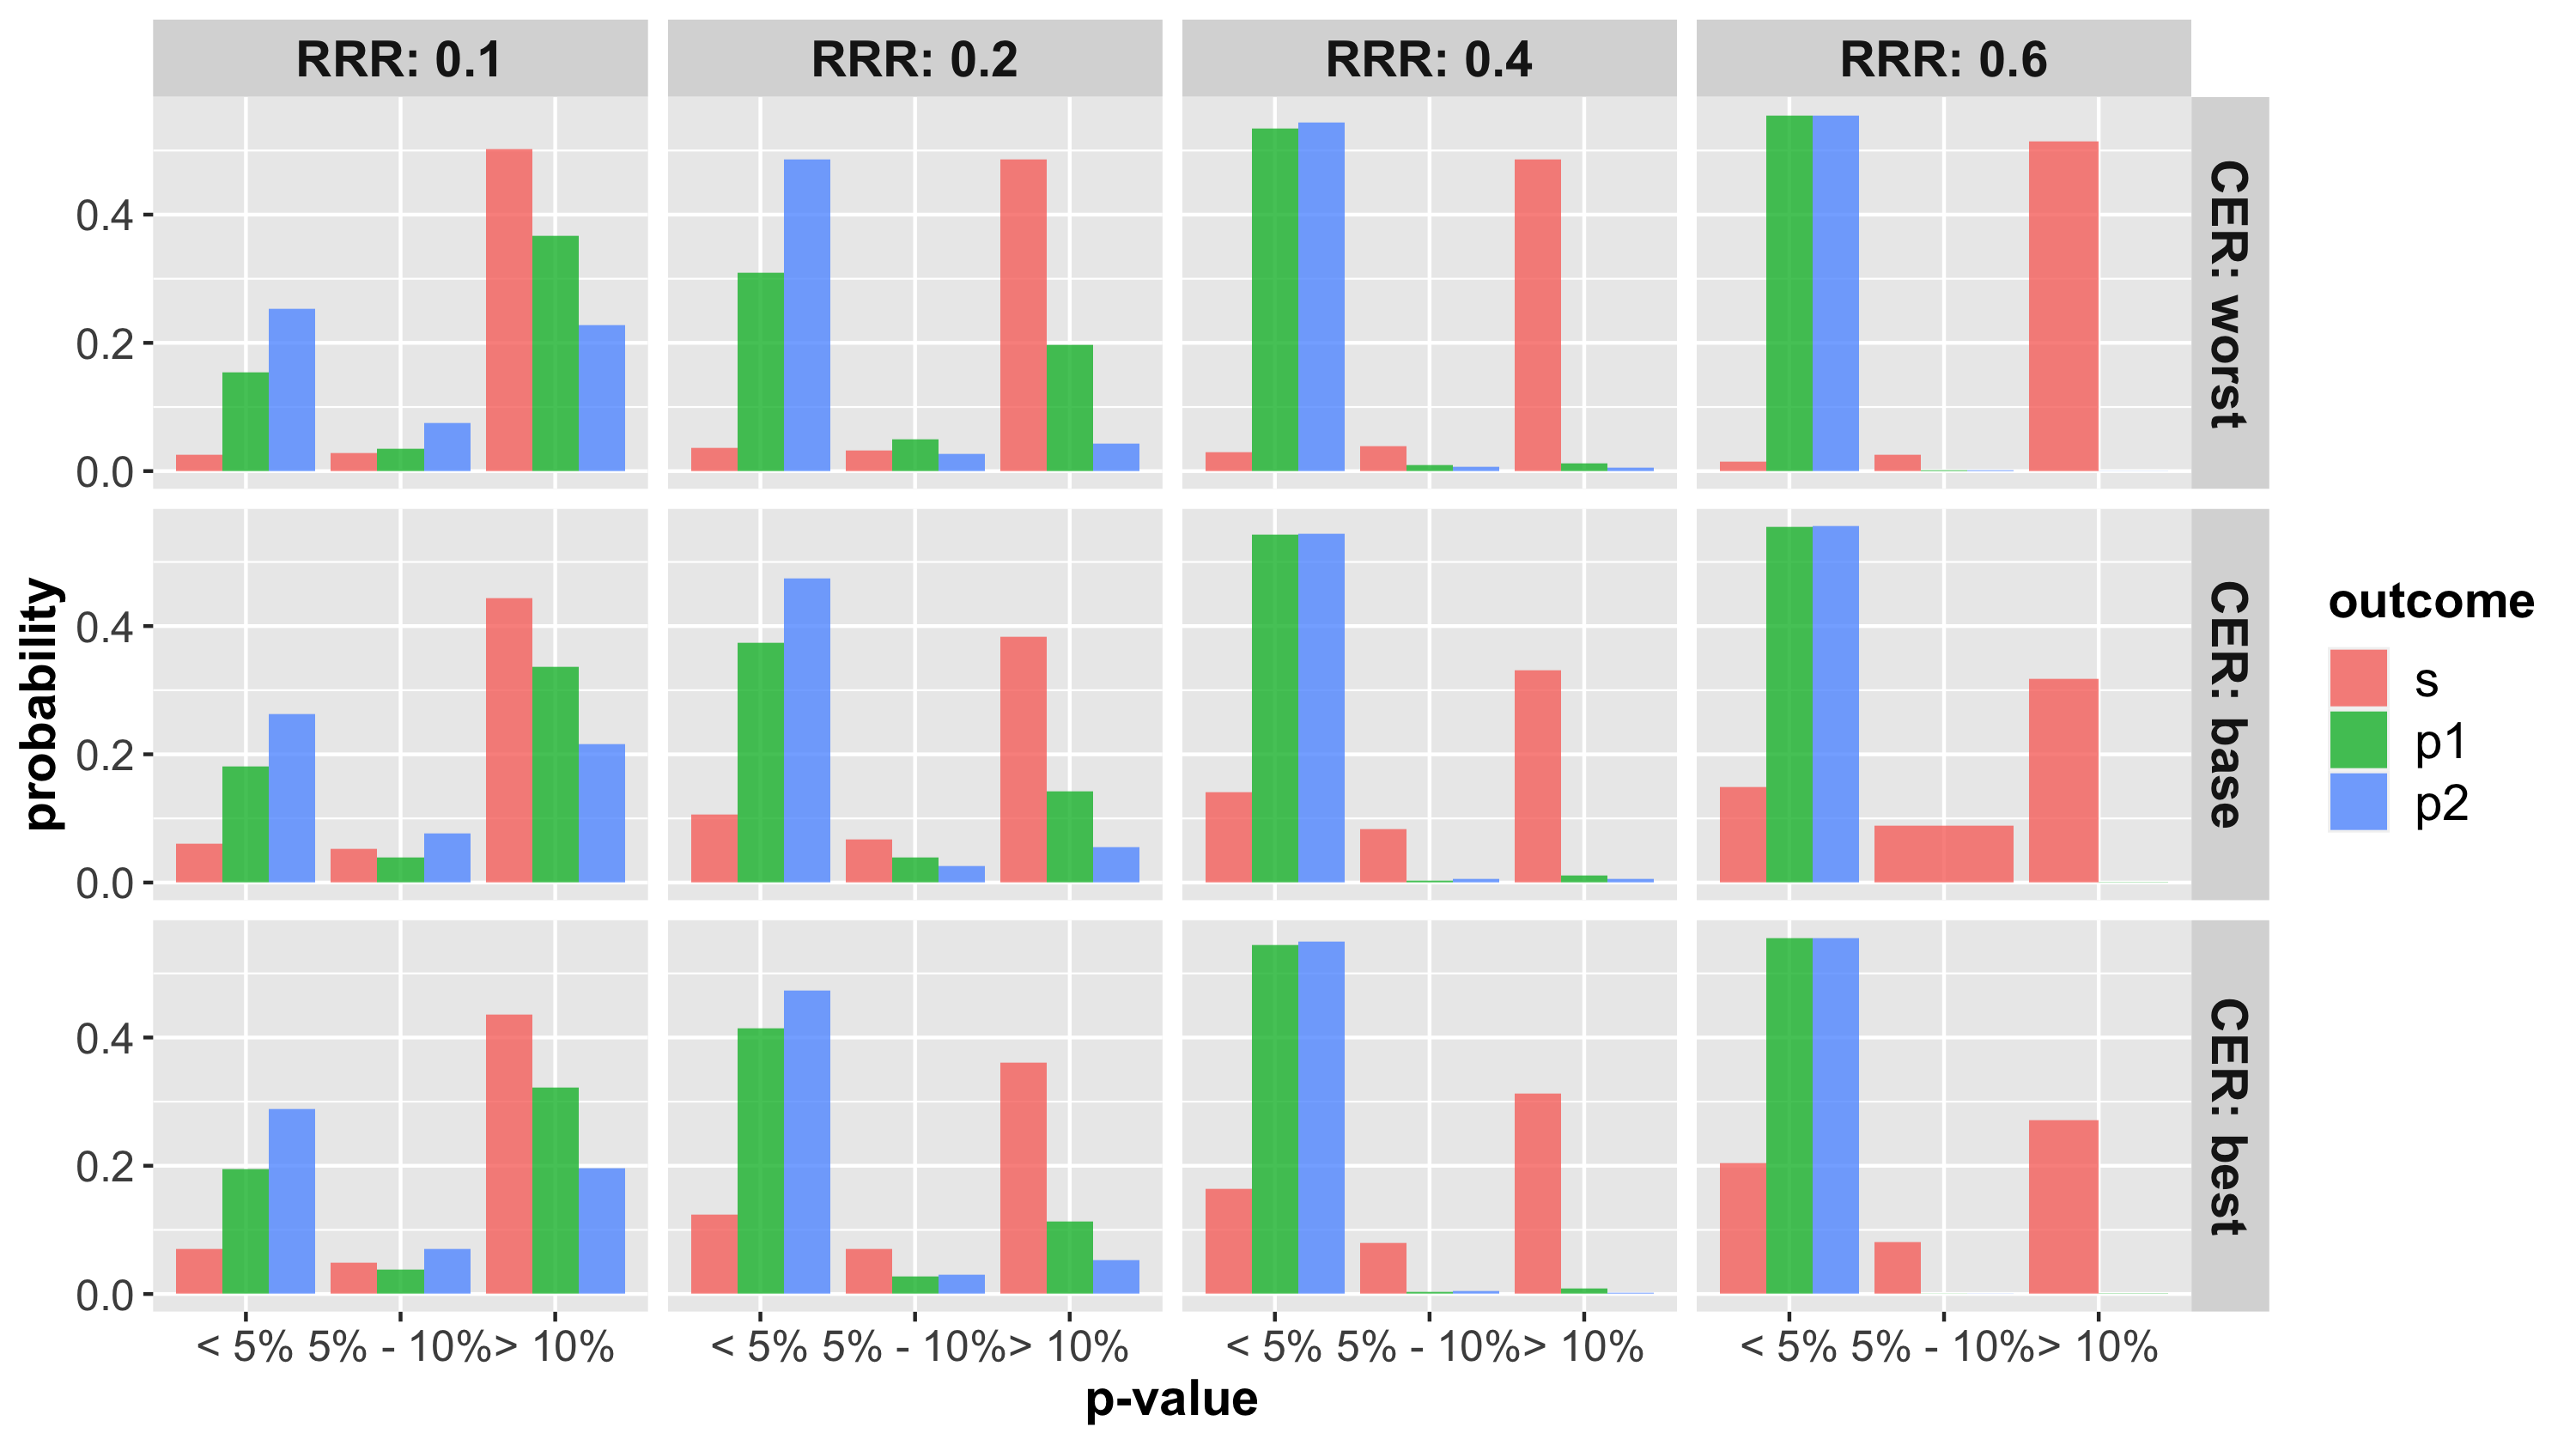
\includegraphics{../p1_plots/batch_size_nb_1000/pvalue_p1.png}
\end{figure}

In the situations where the trial is stopped early for futility, the
small counts for RRR=40\% and 60\% can be explained by the low
probability of stopping early for futility under these scenarios (Figure
7(a)). When the trial is stopped for superiority when the true RRR=40\%
or 60\%, close to 100\% of all p-values for outcomes p1 and p2 are
smaller than 5\%. Under all RRR and CER scenarios, the majority of
p-values for outcomes s remain greater than 10\%.

\begin{figure}
\centering
  \caption{Probability that the p-value (from Fisher’s exact test) at termination of the trial is below 5\%, between 5\%
  and 10\% and greater than 10\% for cases where trial was (a) stopped for futility; (b) stopped for superiority. The
  rows represent the three control even rate scenarios and the three columns present the three relative risk reduction
  scenarios. Note: the denominator in each figure is the number of simulations (not the number of trials stopped for
  futility (a) or superiority (b), and thus, the proportions do not add up to 100\% within one figure. Further, (a) and
  (b) do not include simulations where the trial went to the max. allowed sample size. The bars should be interpreted
  with respect to the relative proportion that fit in each category.}
  \begin{subfigure}{0.8\textwidth}
    \centering
    \caption{}
    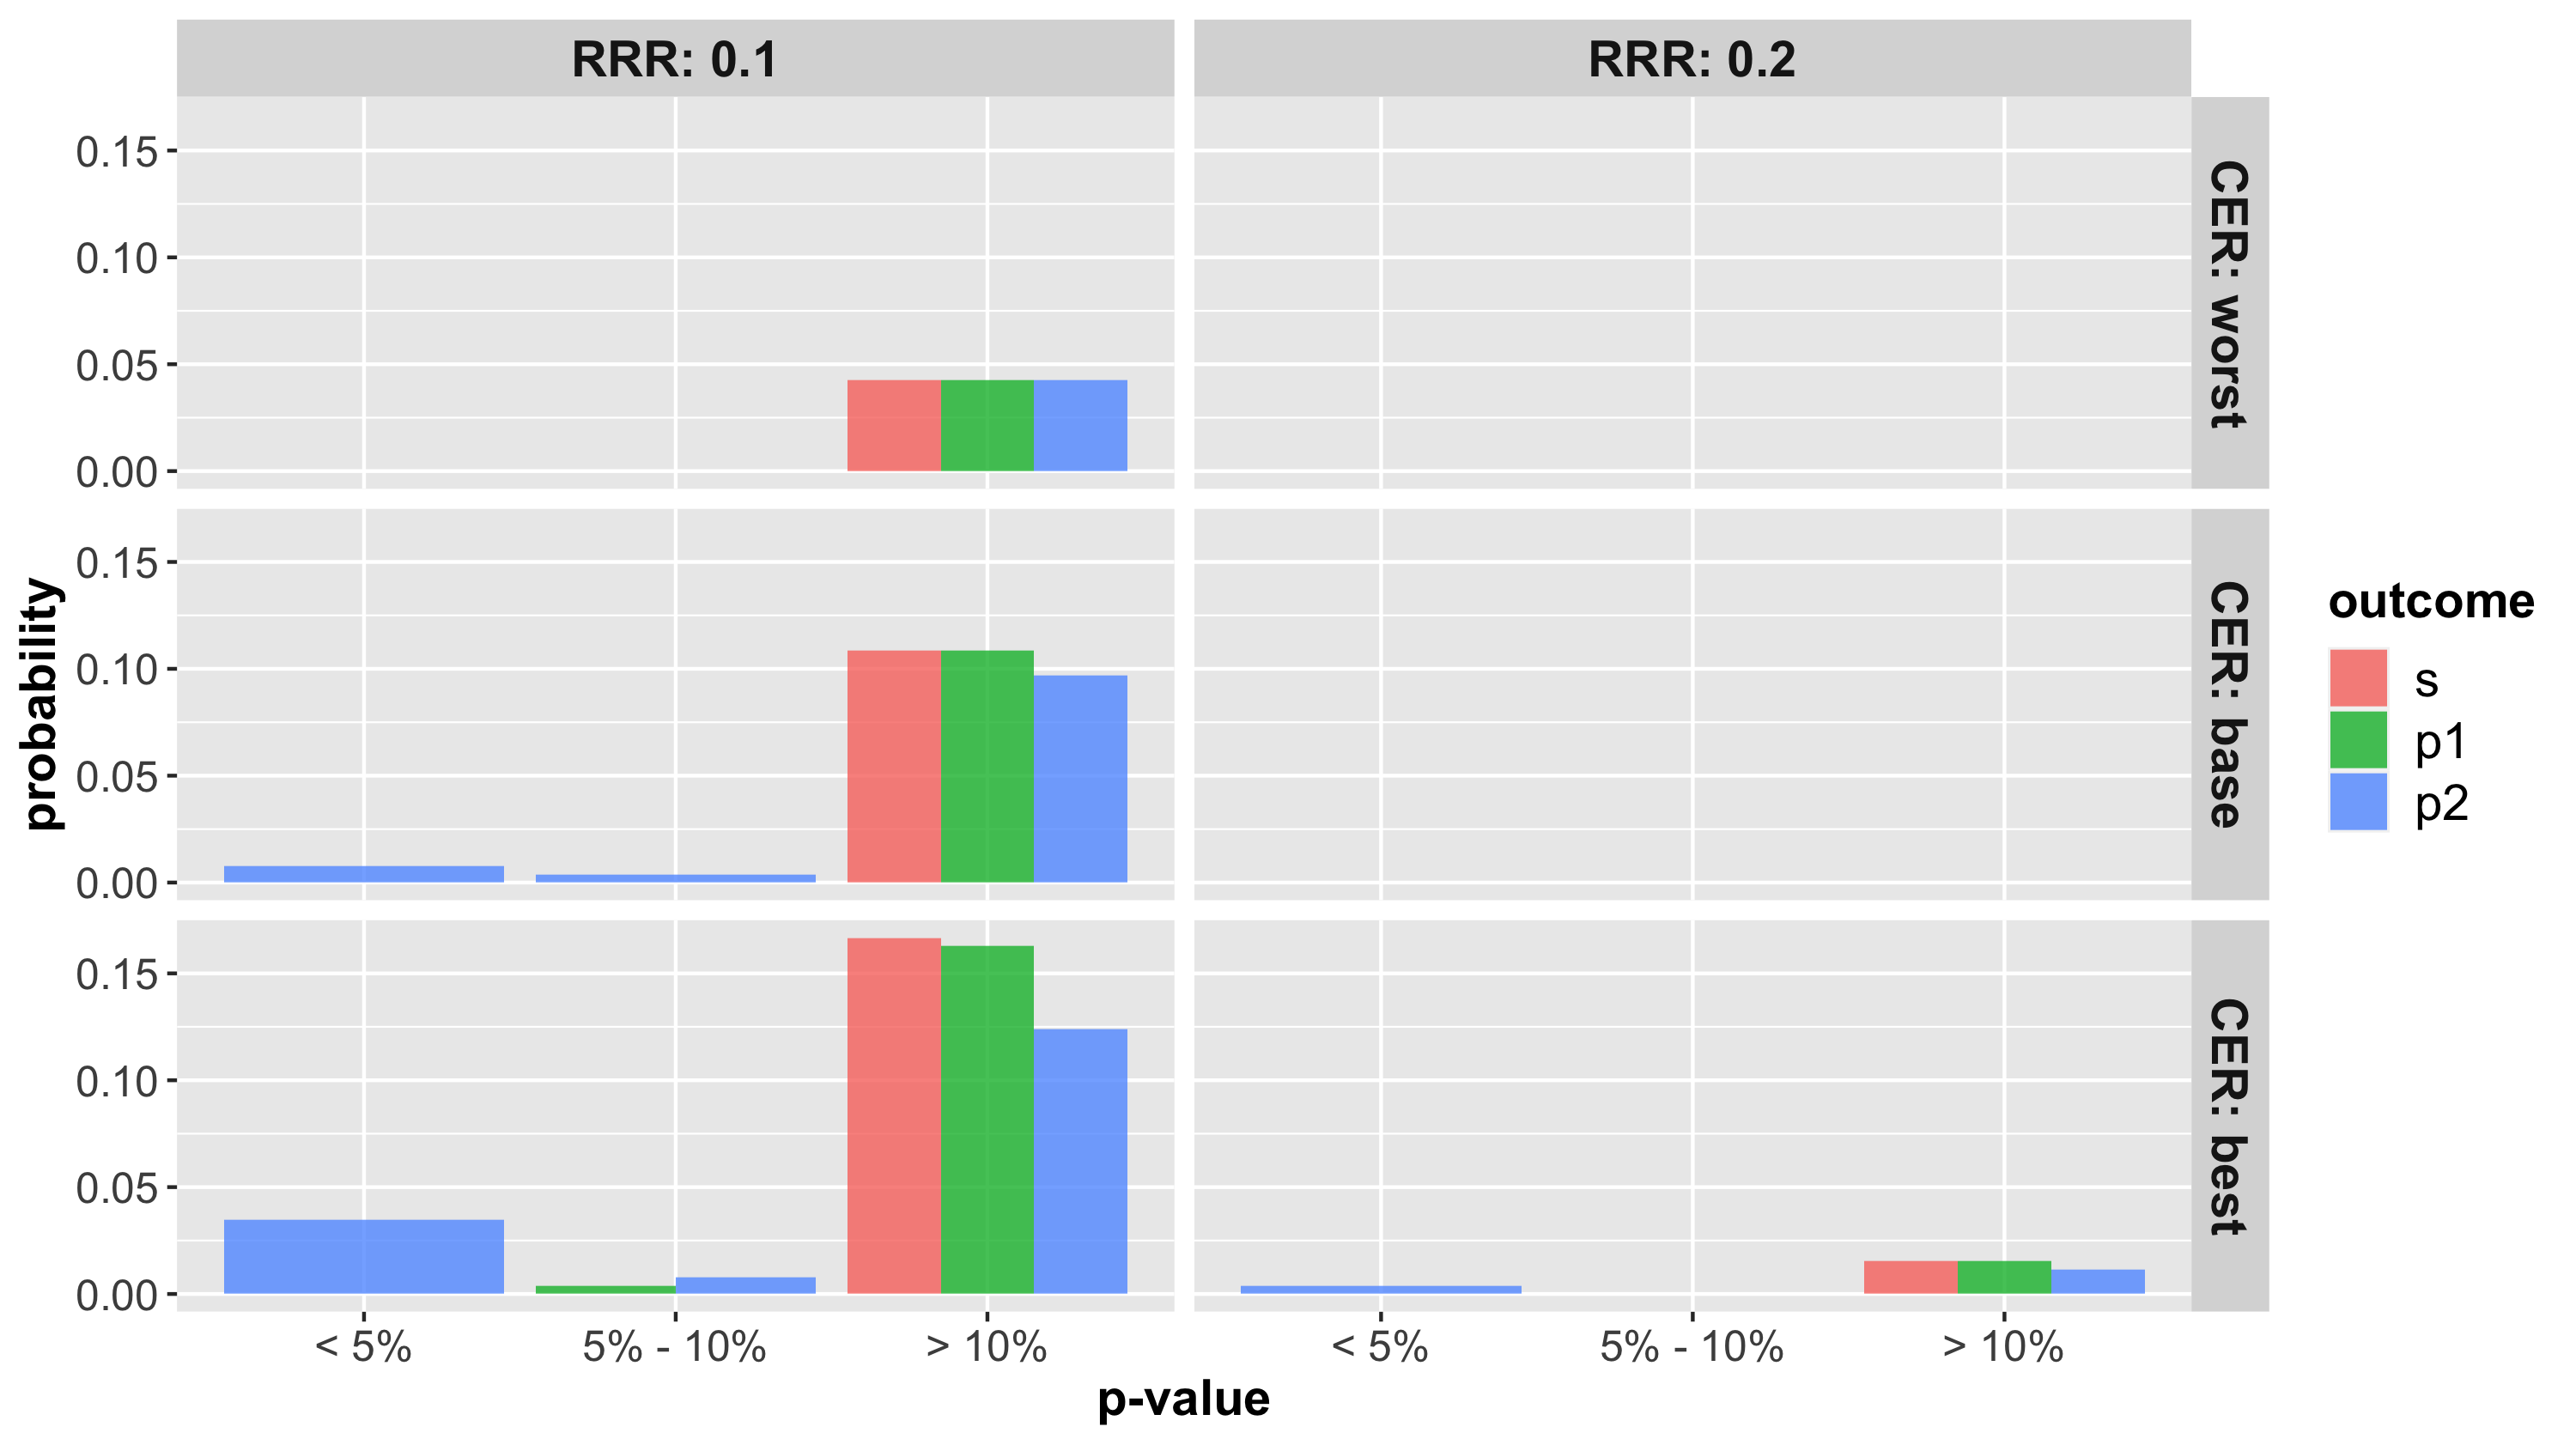
\includegraphics{../p1_plots/batch_size_nb_1000/pvalue_fut_p1.png}
  \end{subfigure}
  \bigbreak
  \begin{subfigure}{0.8\textwidth}
    \centering
    \caption{}
    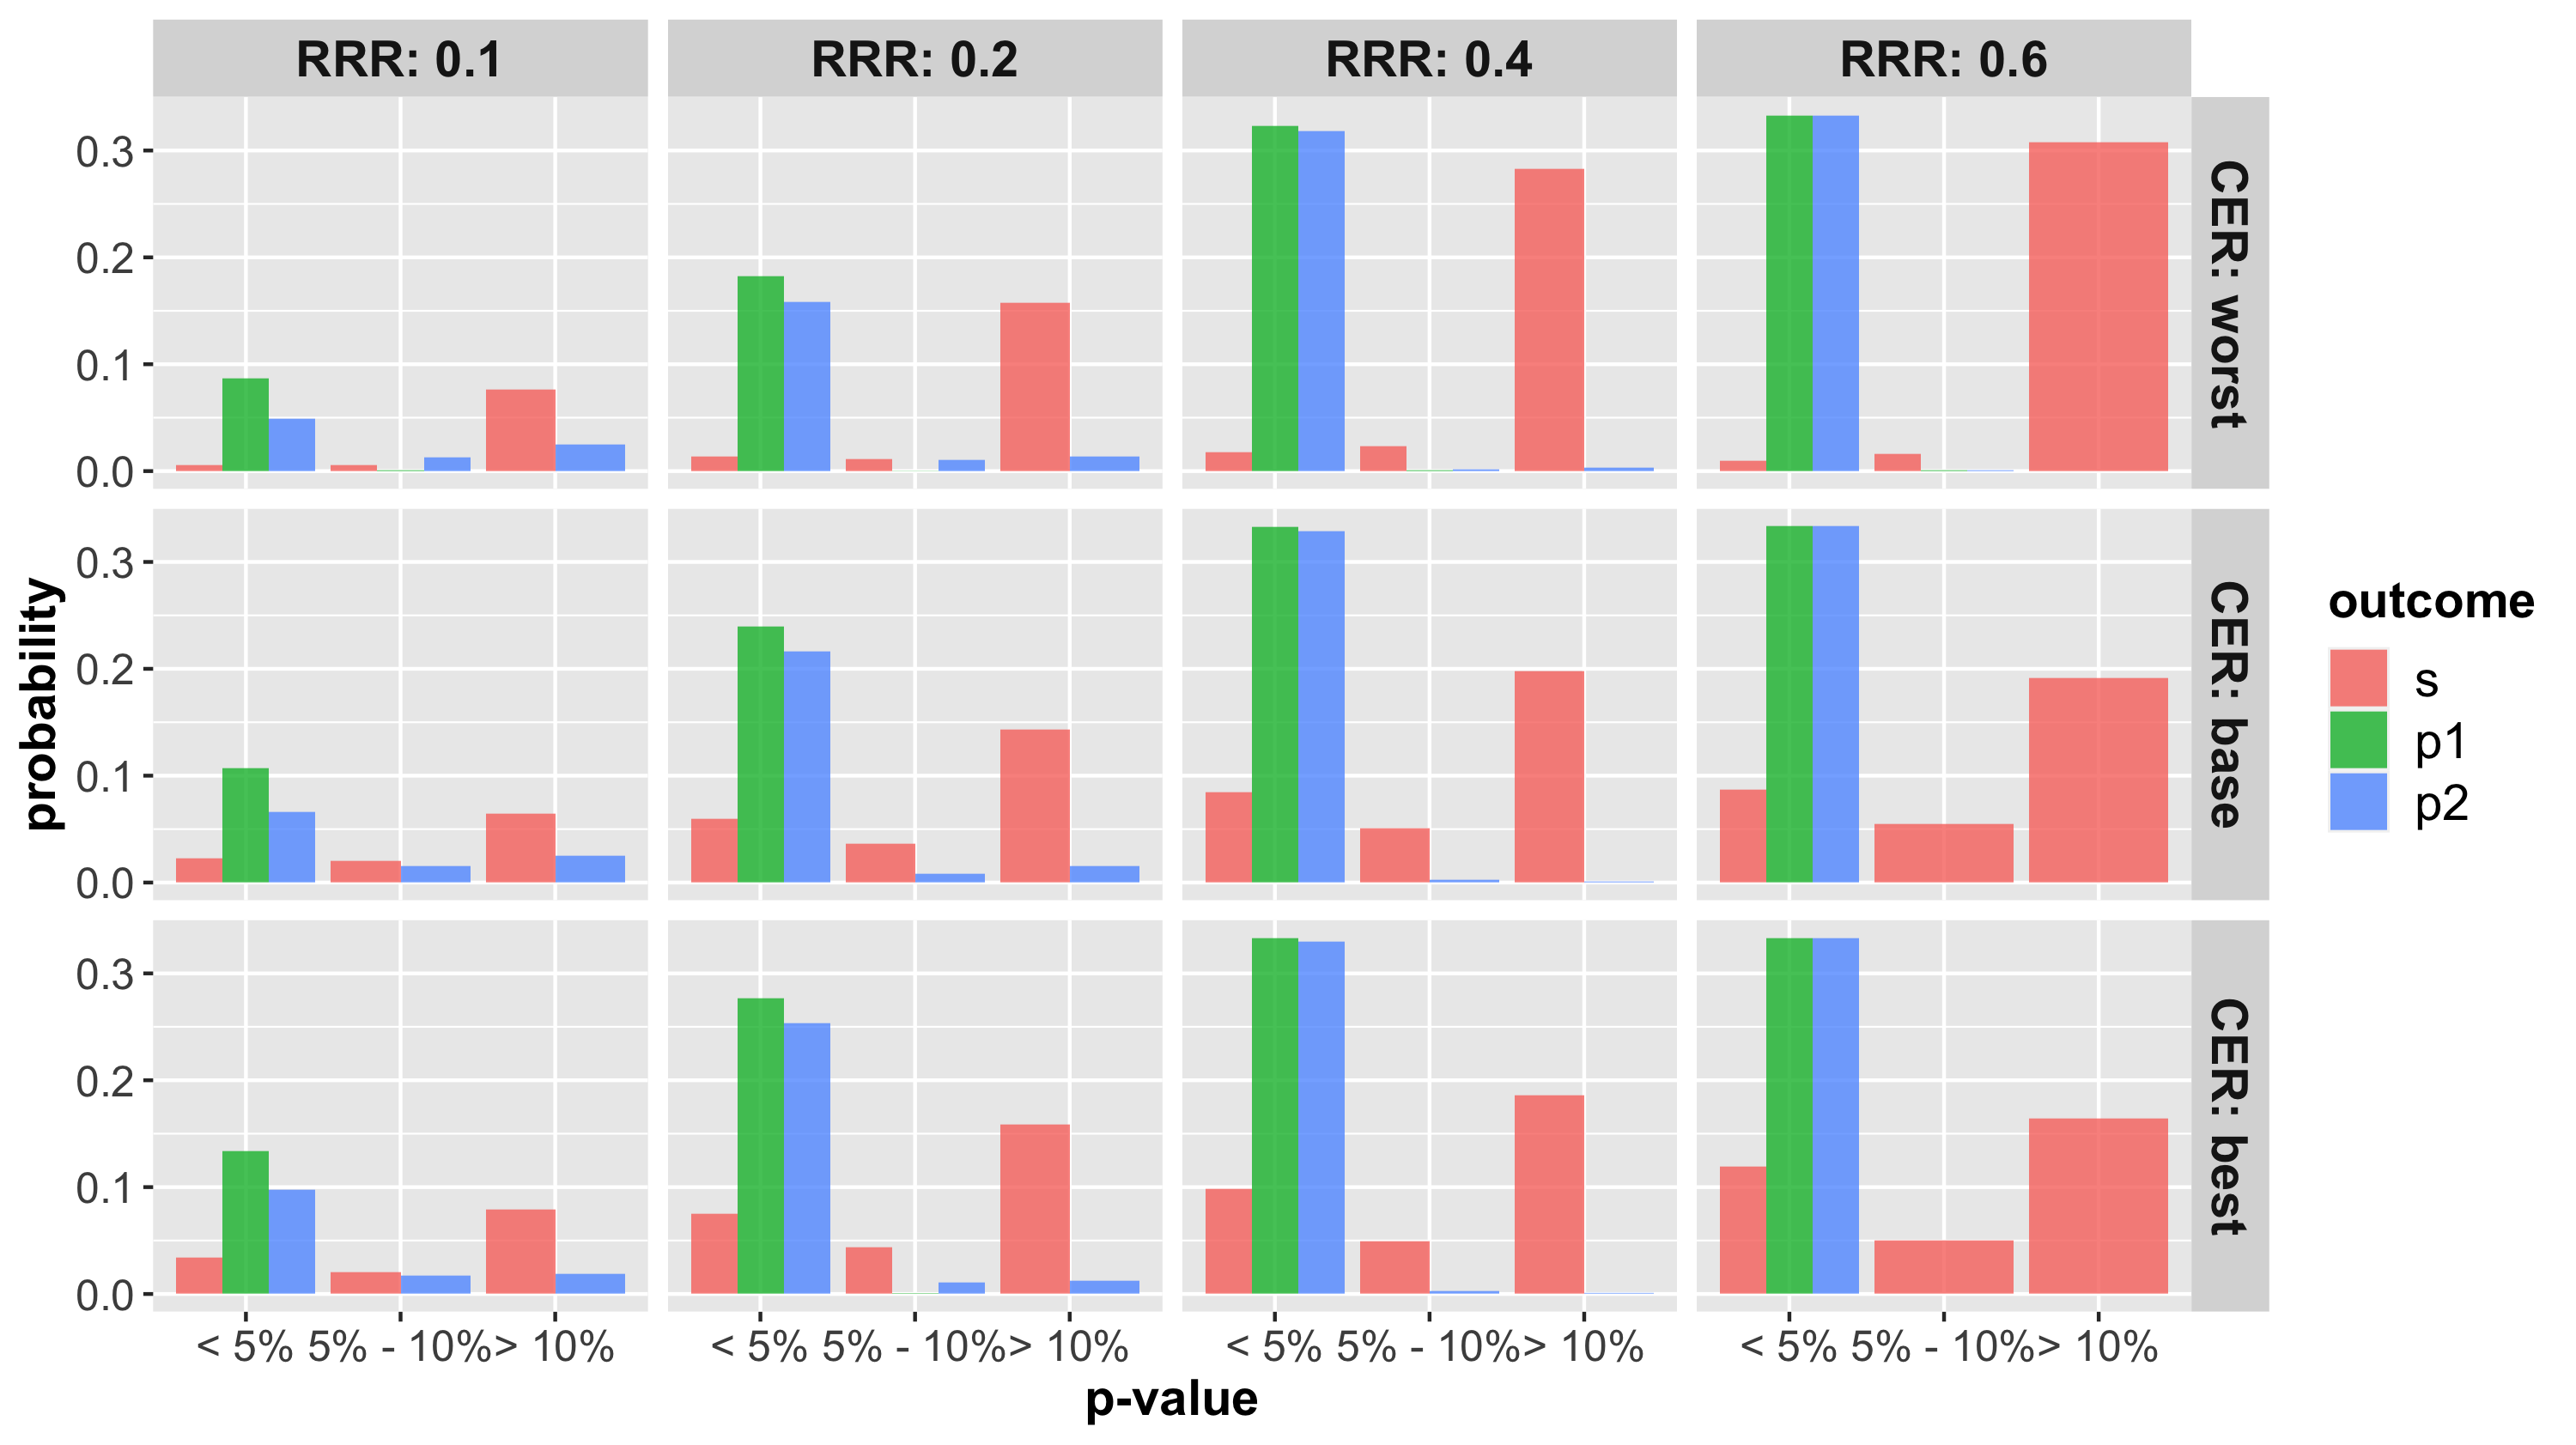
\includegraphics{../p1_plots/batch_size_nb_1000/pvalue_sup_p1.png}
  \end{subfigure}
\end{figure}

\hypertarget{relative-risk-reduction-estimates-at-trial-termination}{%
\paragraph{Relative risk reduction estimates at trial
termination}\label{relative-risk-reduction-estimates-at-trial-termination}}

Figure 10 presents the distribution of relative risk reduction estimates
upon trial termination. Figure 11(a) and 11(b) present the distribution
of relative risk reduction estimates from trials stopped early for
futility and superiority, respectively. As expected, the estimates of p1
and p2 exhibit much larger precision.

\begin{figure}
  \caption{Distribution of relative risk reduction estimates (smoothed by a kernel density estimator) for the three
  control event rates (CER – rows), four relative risk reductions (RRR – columns) and the three outcomes (legend).}
  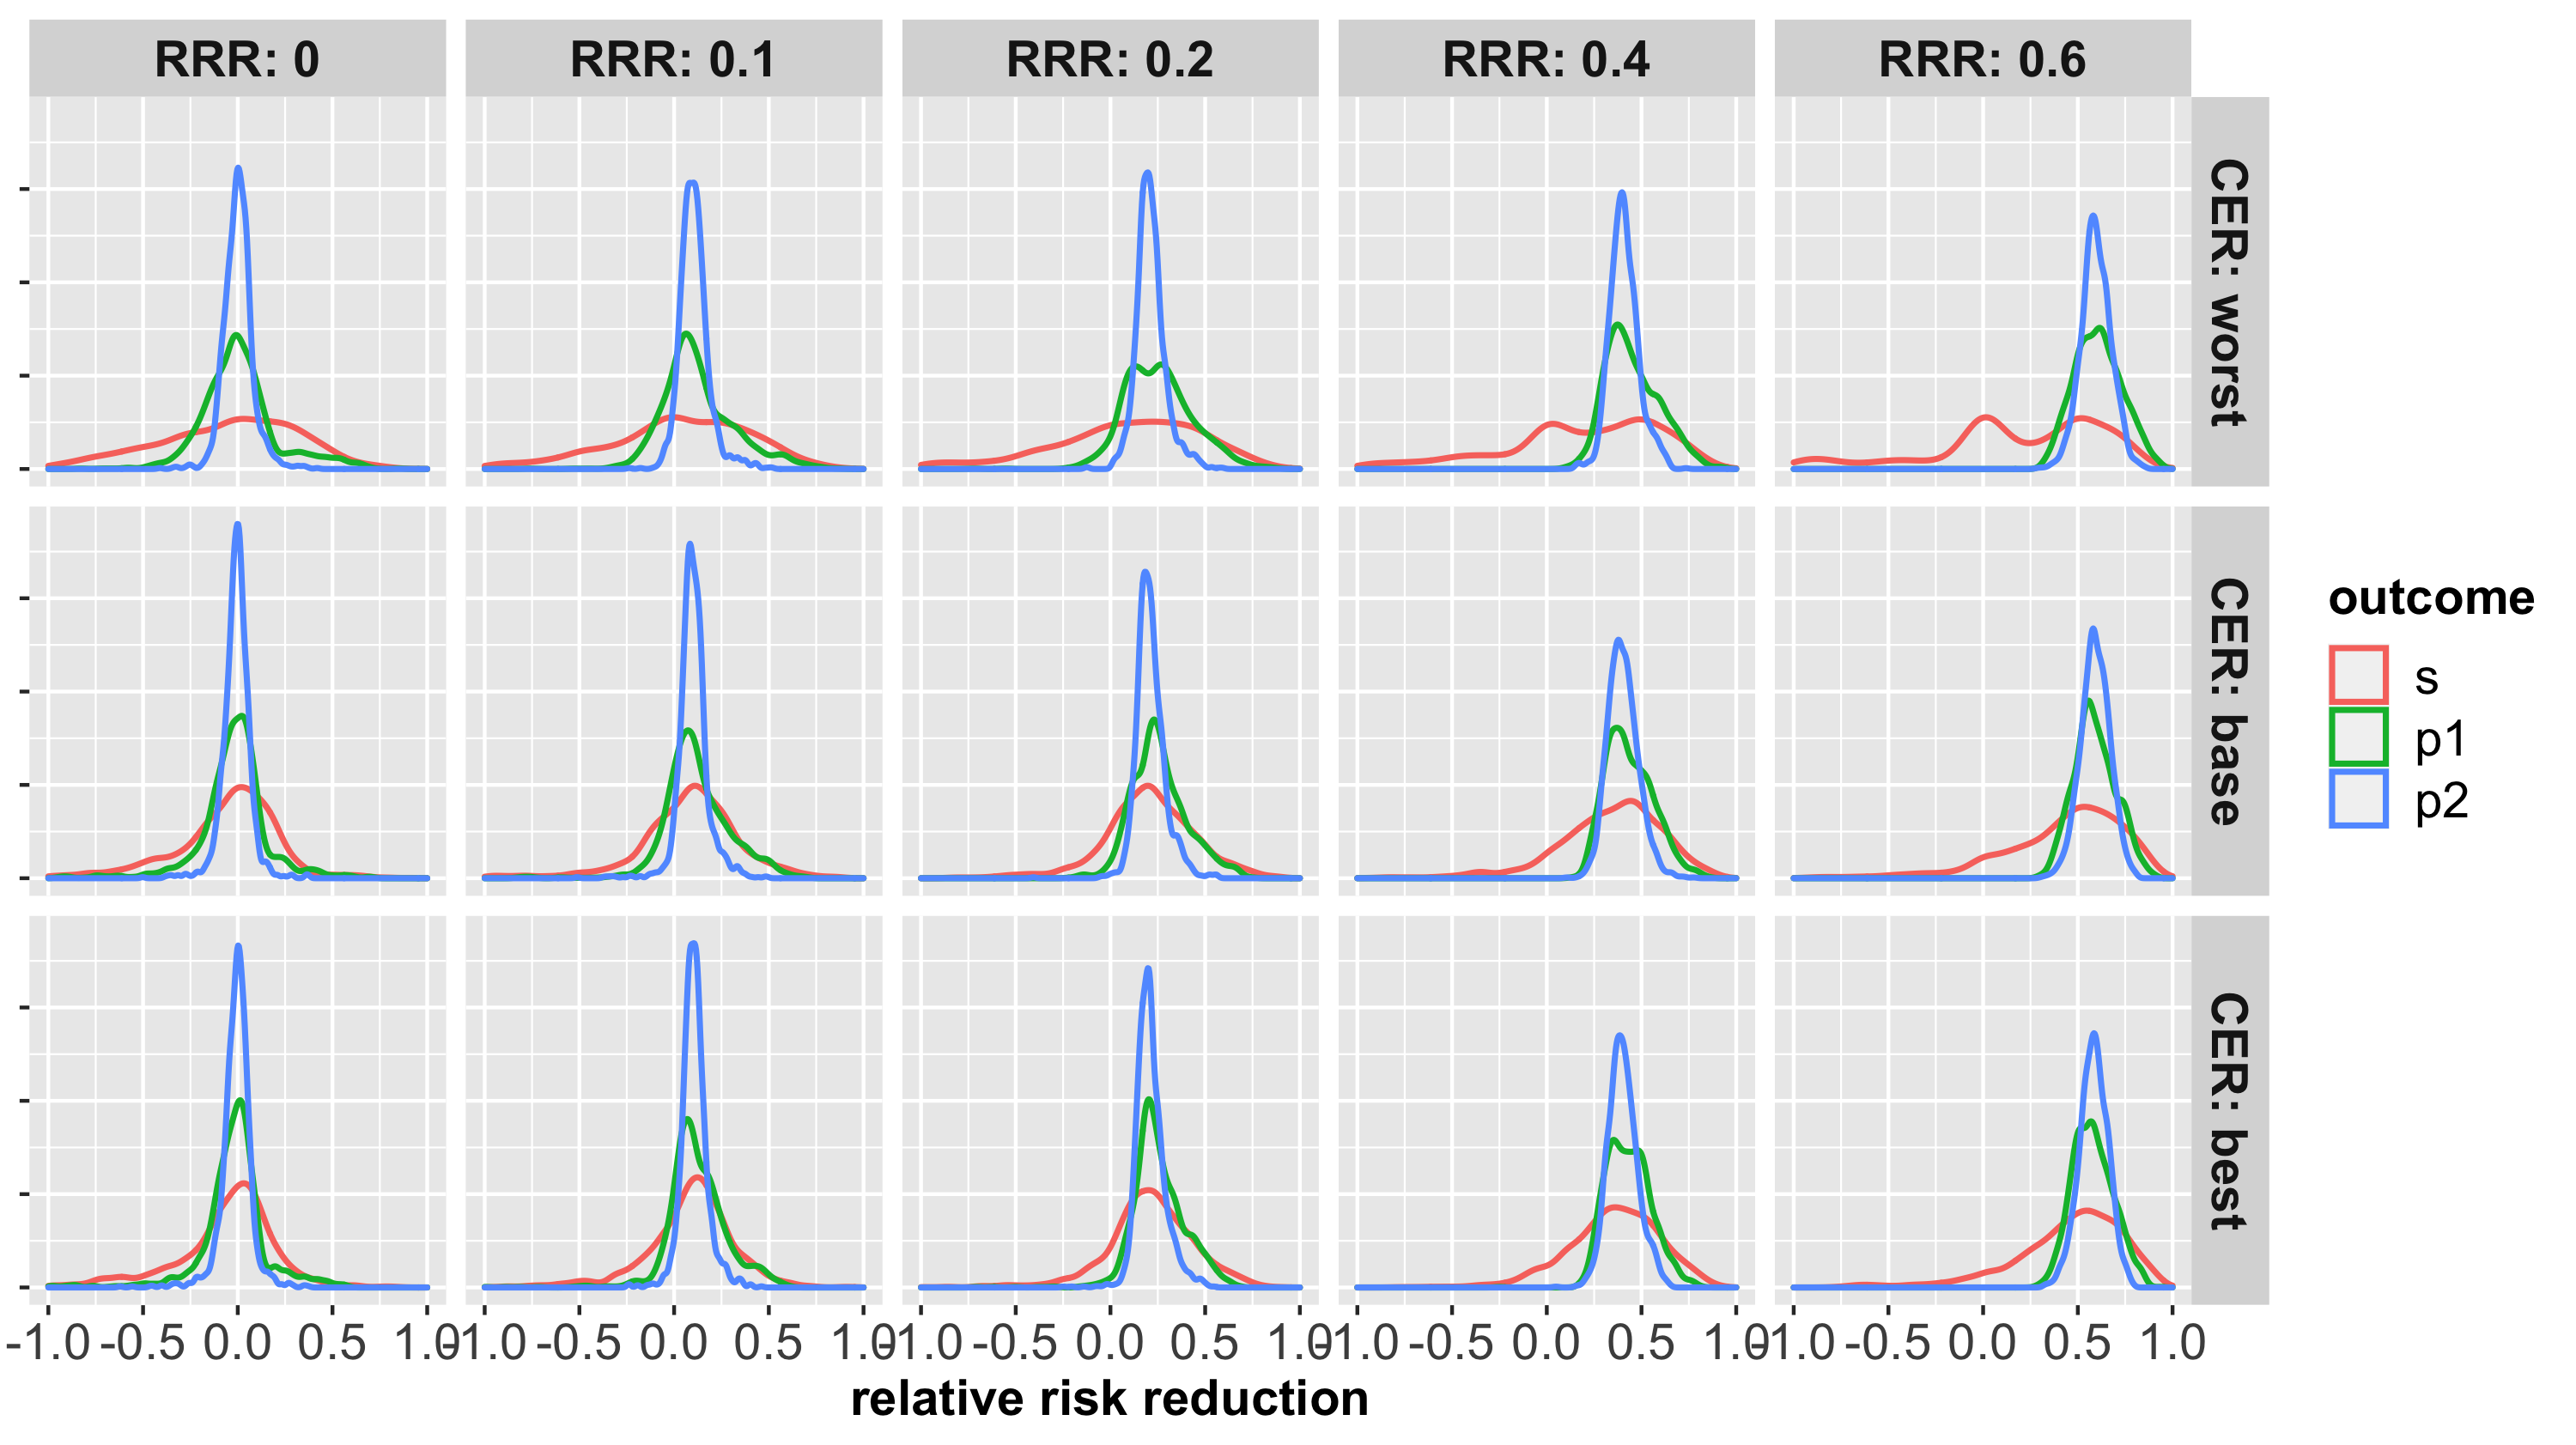
\includegraphics{../p1_plots/batch_size_nb_1000/RRRhat_p1.png}
\end{figure}

When stopping for futility, outcome s incurs small to moderate downward
bias for all scenarios. For true RRR=0 and 20\% and across all CER
scenarios, both outcomes p1 and p2 show negligible bias, though p2 shows
greater precision. When stopping for futility, the estimates for RRR =
40\% and 60\% are unstable, but the kernel density smoother obscures
this. When stopping for superiority, outcome s is very diffuse in the
worst case CER scenario, but sees its precision improve with the CER. It
has marginal upward bias when the true RRR=0 and 20\%, but shows little
bias for true RRR=40\% and 60\% for the base and best case CER
scenarios. Outcome p2 has greatest precision across all scenarios and
has negligible bias. Outcome p1 has moderate to good precision across
all scenarios but has moderate upward bias for true RRR=0, 10\%, and
20\%.

\begin{figure}
\centering
  \caption{Distribution of relative risk reduction estimates after stopping early for (a) futility; (b) superiority.
  Results are presented for the three control event rates by rows, four relative risk reductions (by columns) and the
  three outcomes (legend).}
  \begin{subfigure}{0.8\textwidth}
    \centering
    \caption{}
    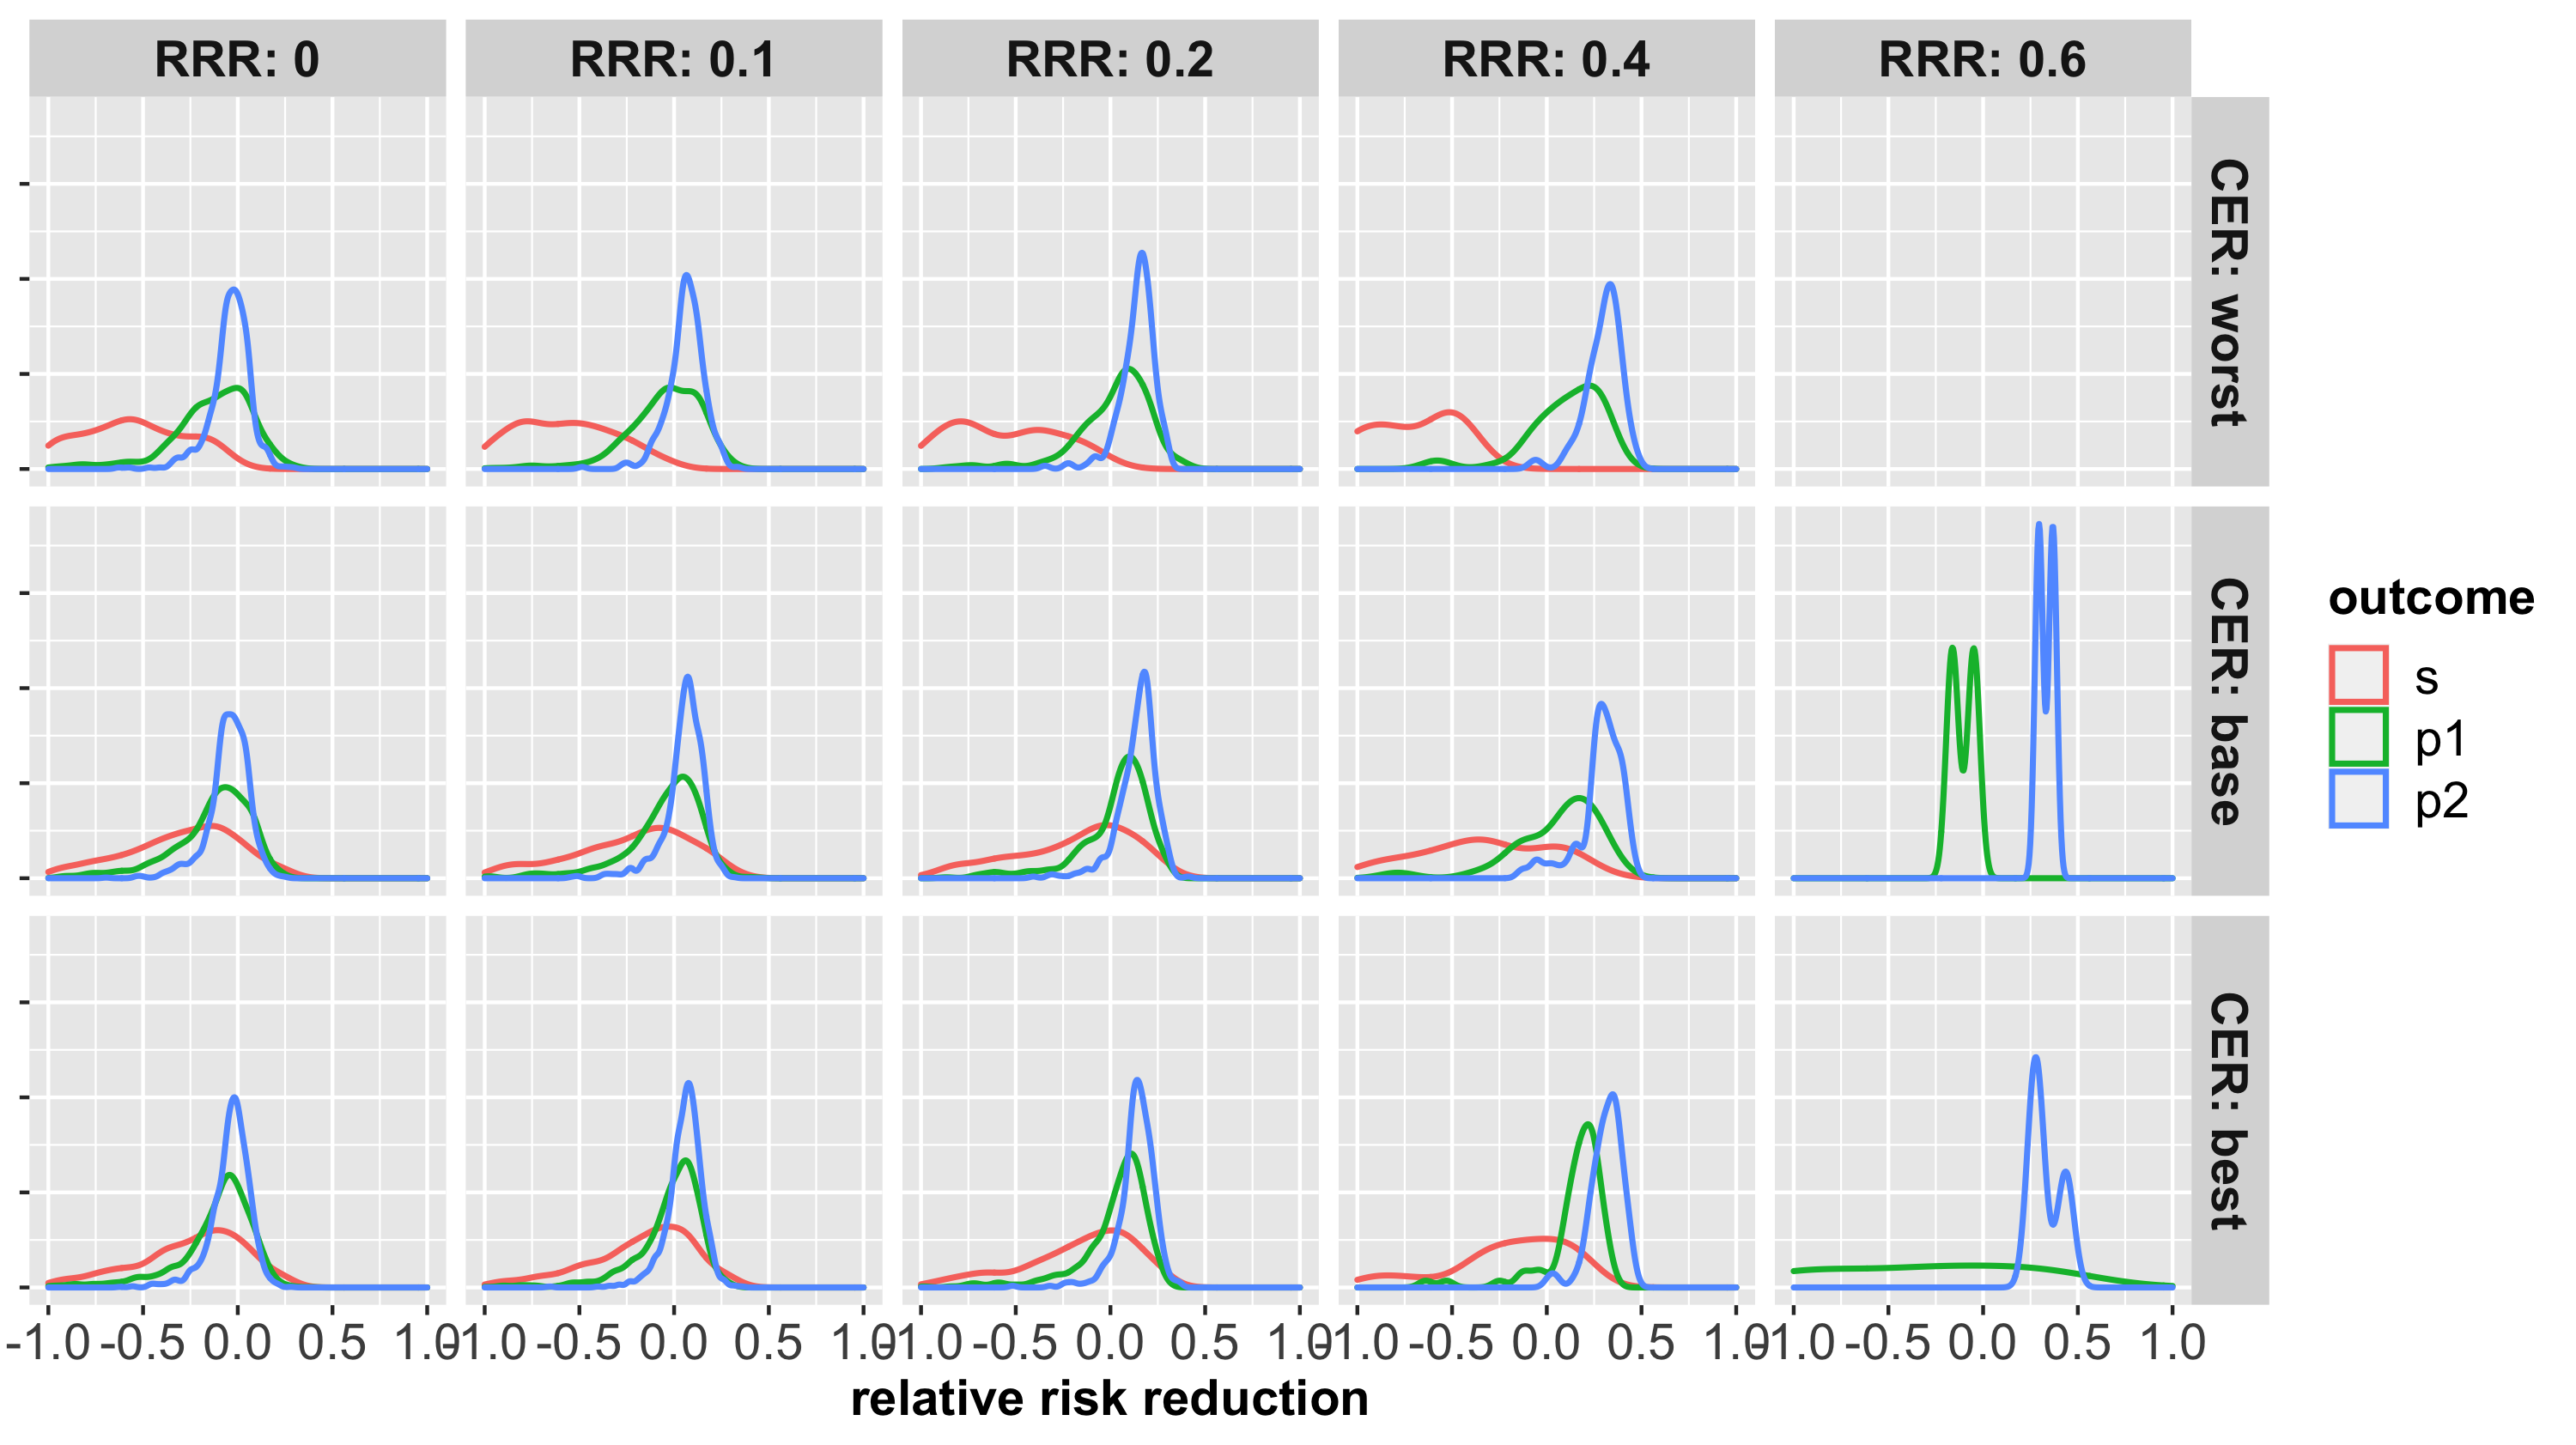
\includegraphics{../p1_plots/batch_size_nb_1000/RRRhat_fut_p1.png}
  \end{subfigure}
  \bigbreak
  \begin{subfigure}{0.8\textwidth}
    \centering
    \caption{}
    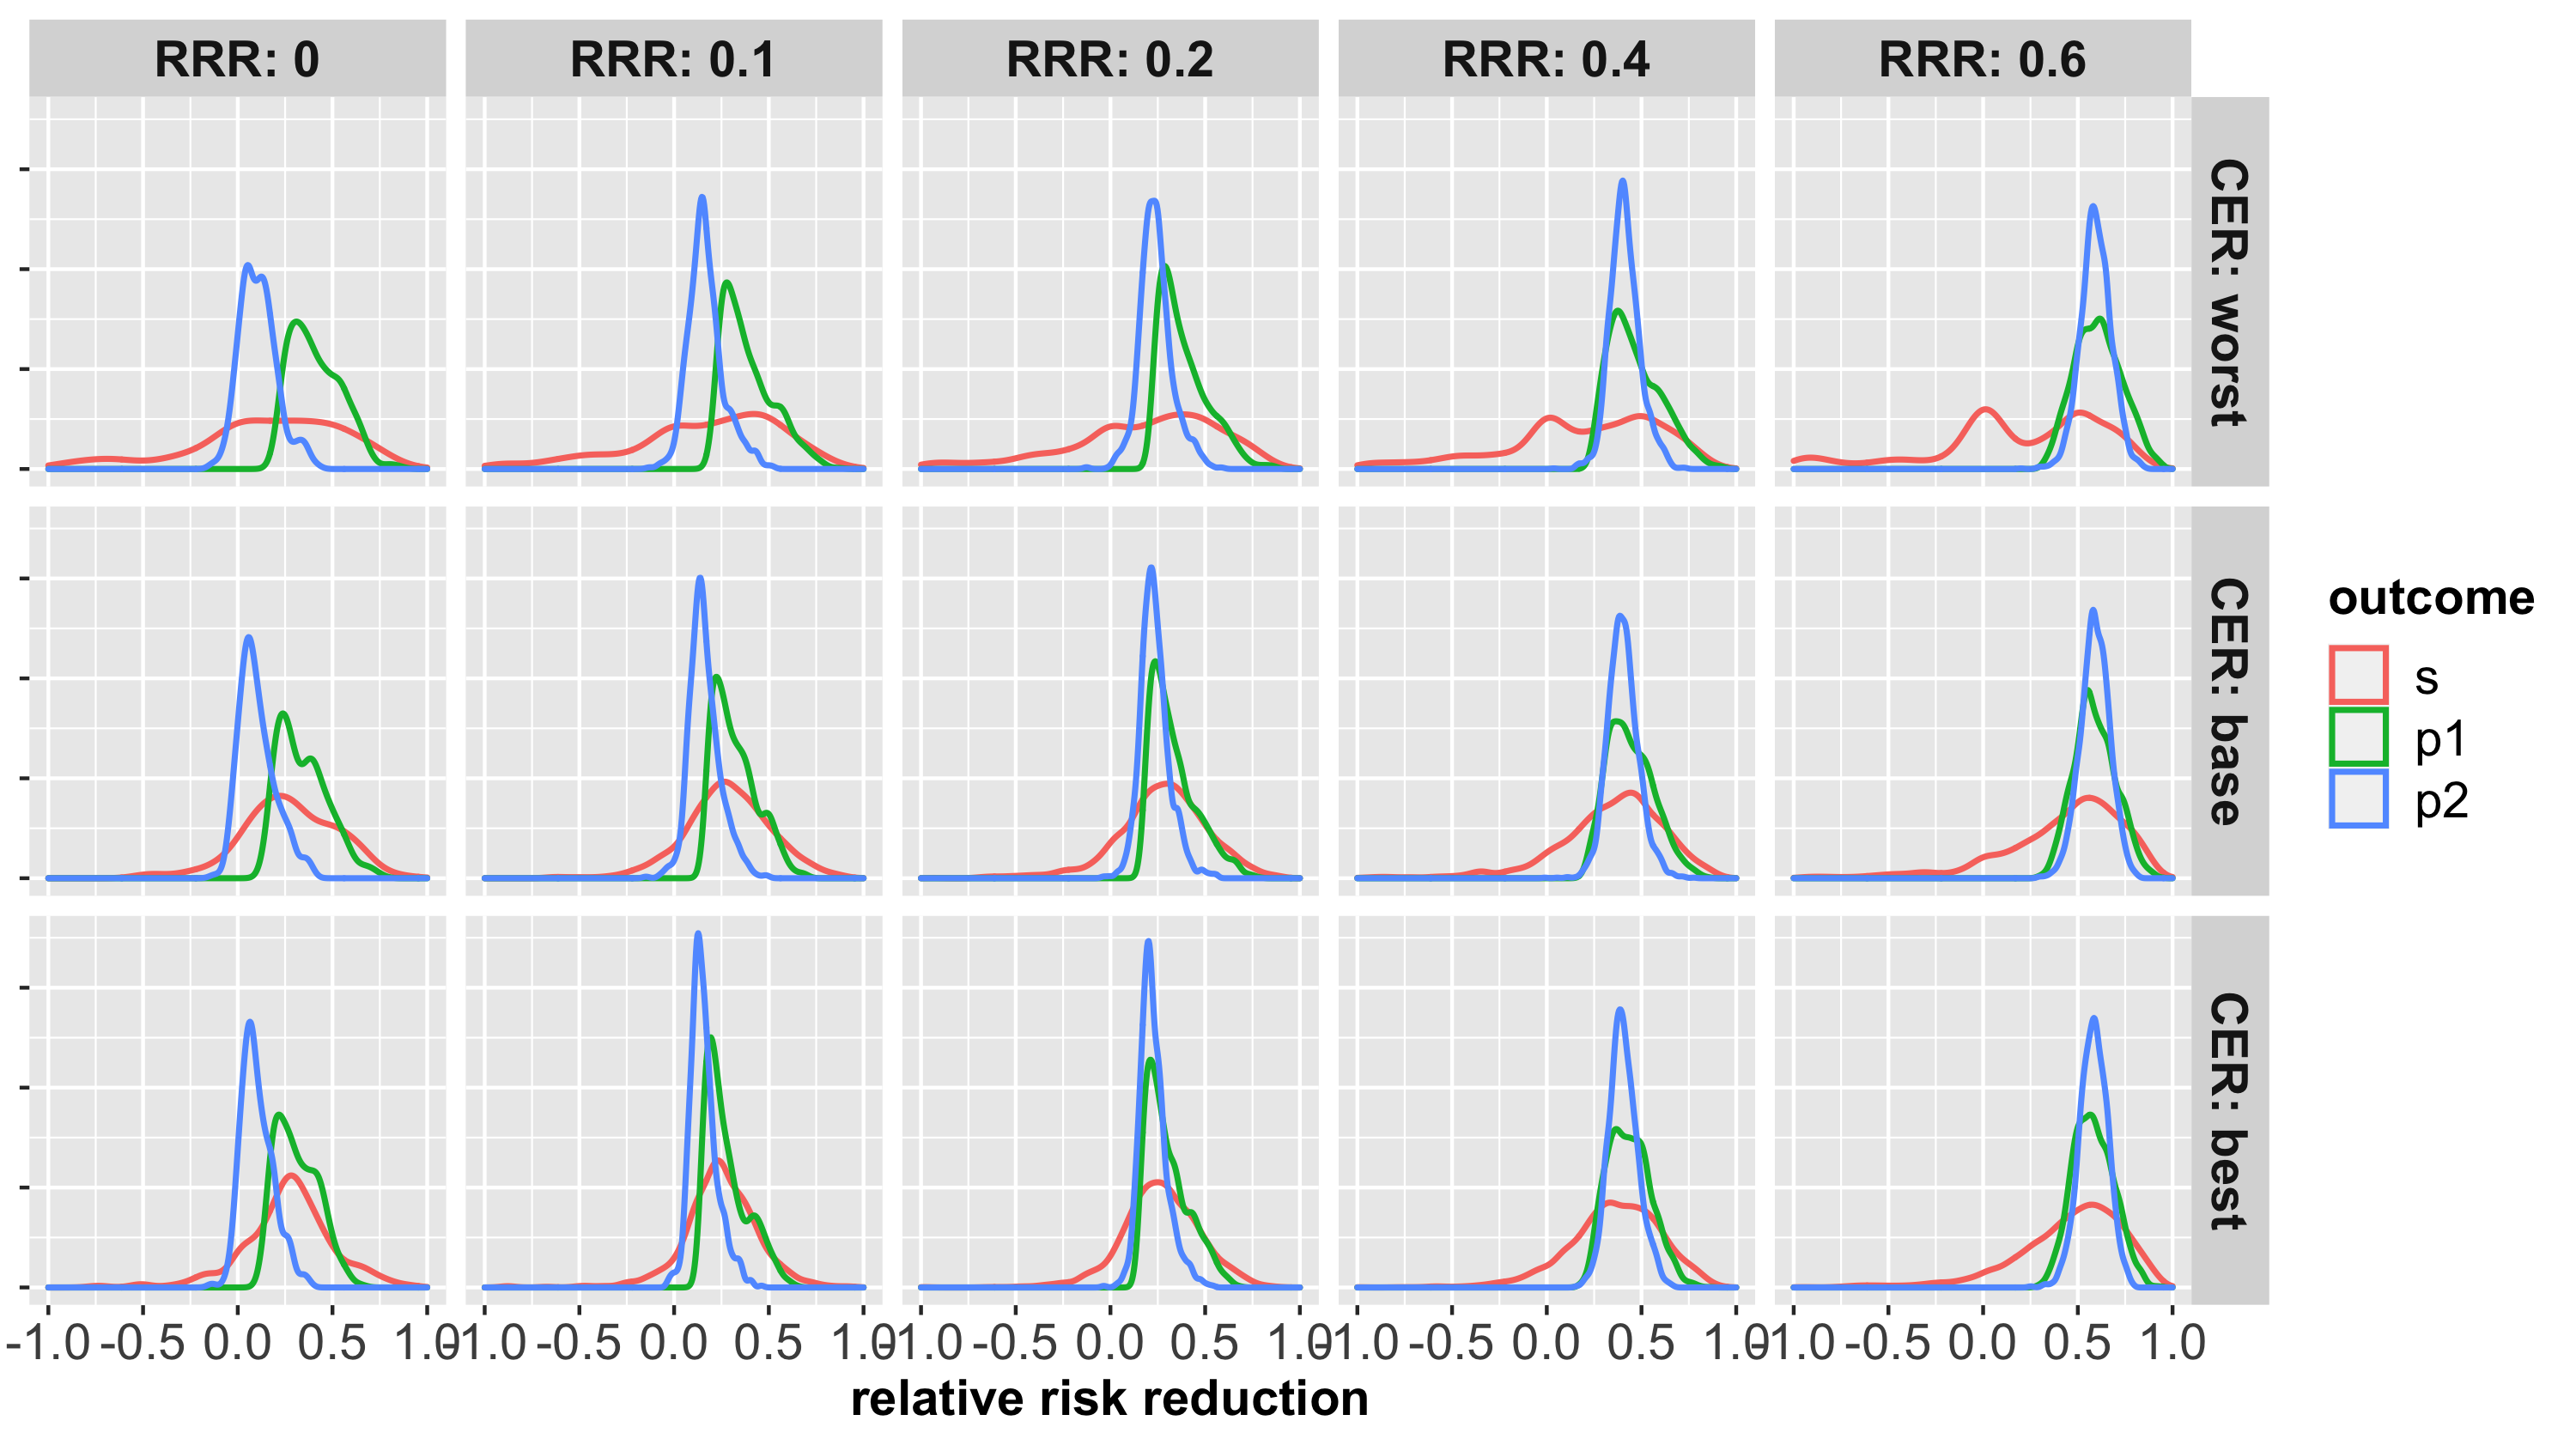
\includegraphics{../p1_plots/batch_size_nb_1000/RRRhat_sup_p1.png}
  \end{subfigure}
\end{figure}

\hypertarget{stopping-with-moderately-permissive-outcome-p1-1}{%
\subsection{Stopping with moderately permissive outcome
(p1)}\label{stopping-with-moderately-permissive-outcome-p1-1}}

\hypertarget{maximum-allowed-sample-size-of-12000-with-interim-analyses-conducted-every-2000-patients}{%
\paragraph{Maximum allowed sample size of 12,000 with interim analyses
conducted every 2,000
patients}\label{maximum-allowed-sample-size-of-12000-with-interim-analyses-conducted-every-2000-patients}}

Both superiority and futility decisions were made with respect to the
moderately permissive outcome (p1). Unless stated otherwise, the
futility bound used was 0.4 and a probability threshold of 0.99 was
required to stop for futility. The number of expected interim analyses
can be thought of as the expected number of patients at trial
determination divided by the batch size, which here is 2,000 patients.
The plots below can be interpretated in the same manner as those above.

\hypertarget{type-i-error-false-positive-risk-1}{%
\subparagraph{Type I error (false positive
risk)}\label{type-i-error-false-positive-risk-1}}

\captionsetup[figure]{font=small,labelfont=small}

\begin{figure}
  \caption{Overall type I error rate based on moderately permissive (p1) outcome based stopping rules.Observed type one error rate for each outcome is
  presented by colored bars (see legend). Results by the three categories of control event rates are by rows. Results by the futility thresholds are
  presented on the x-axis.}
  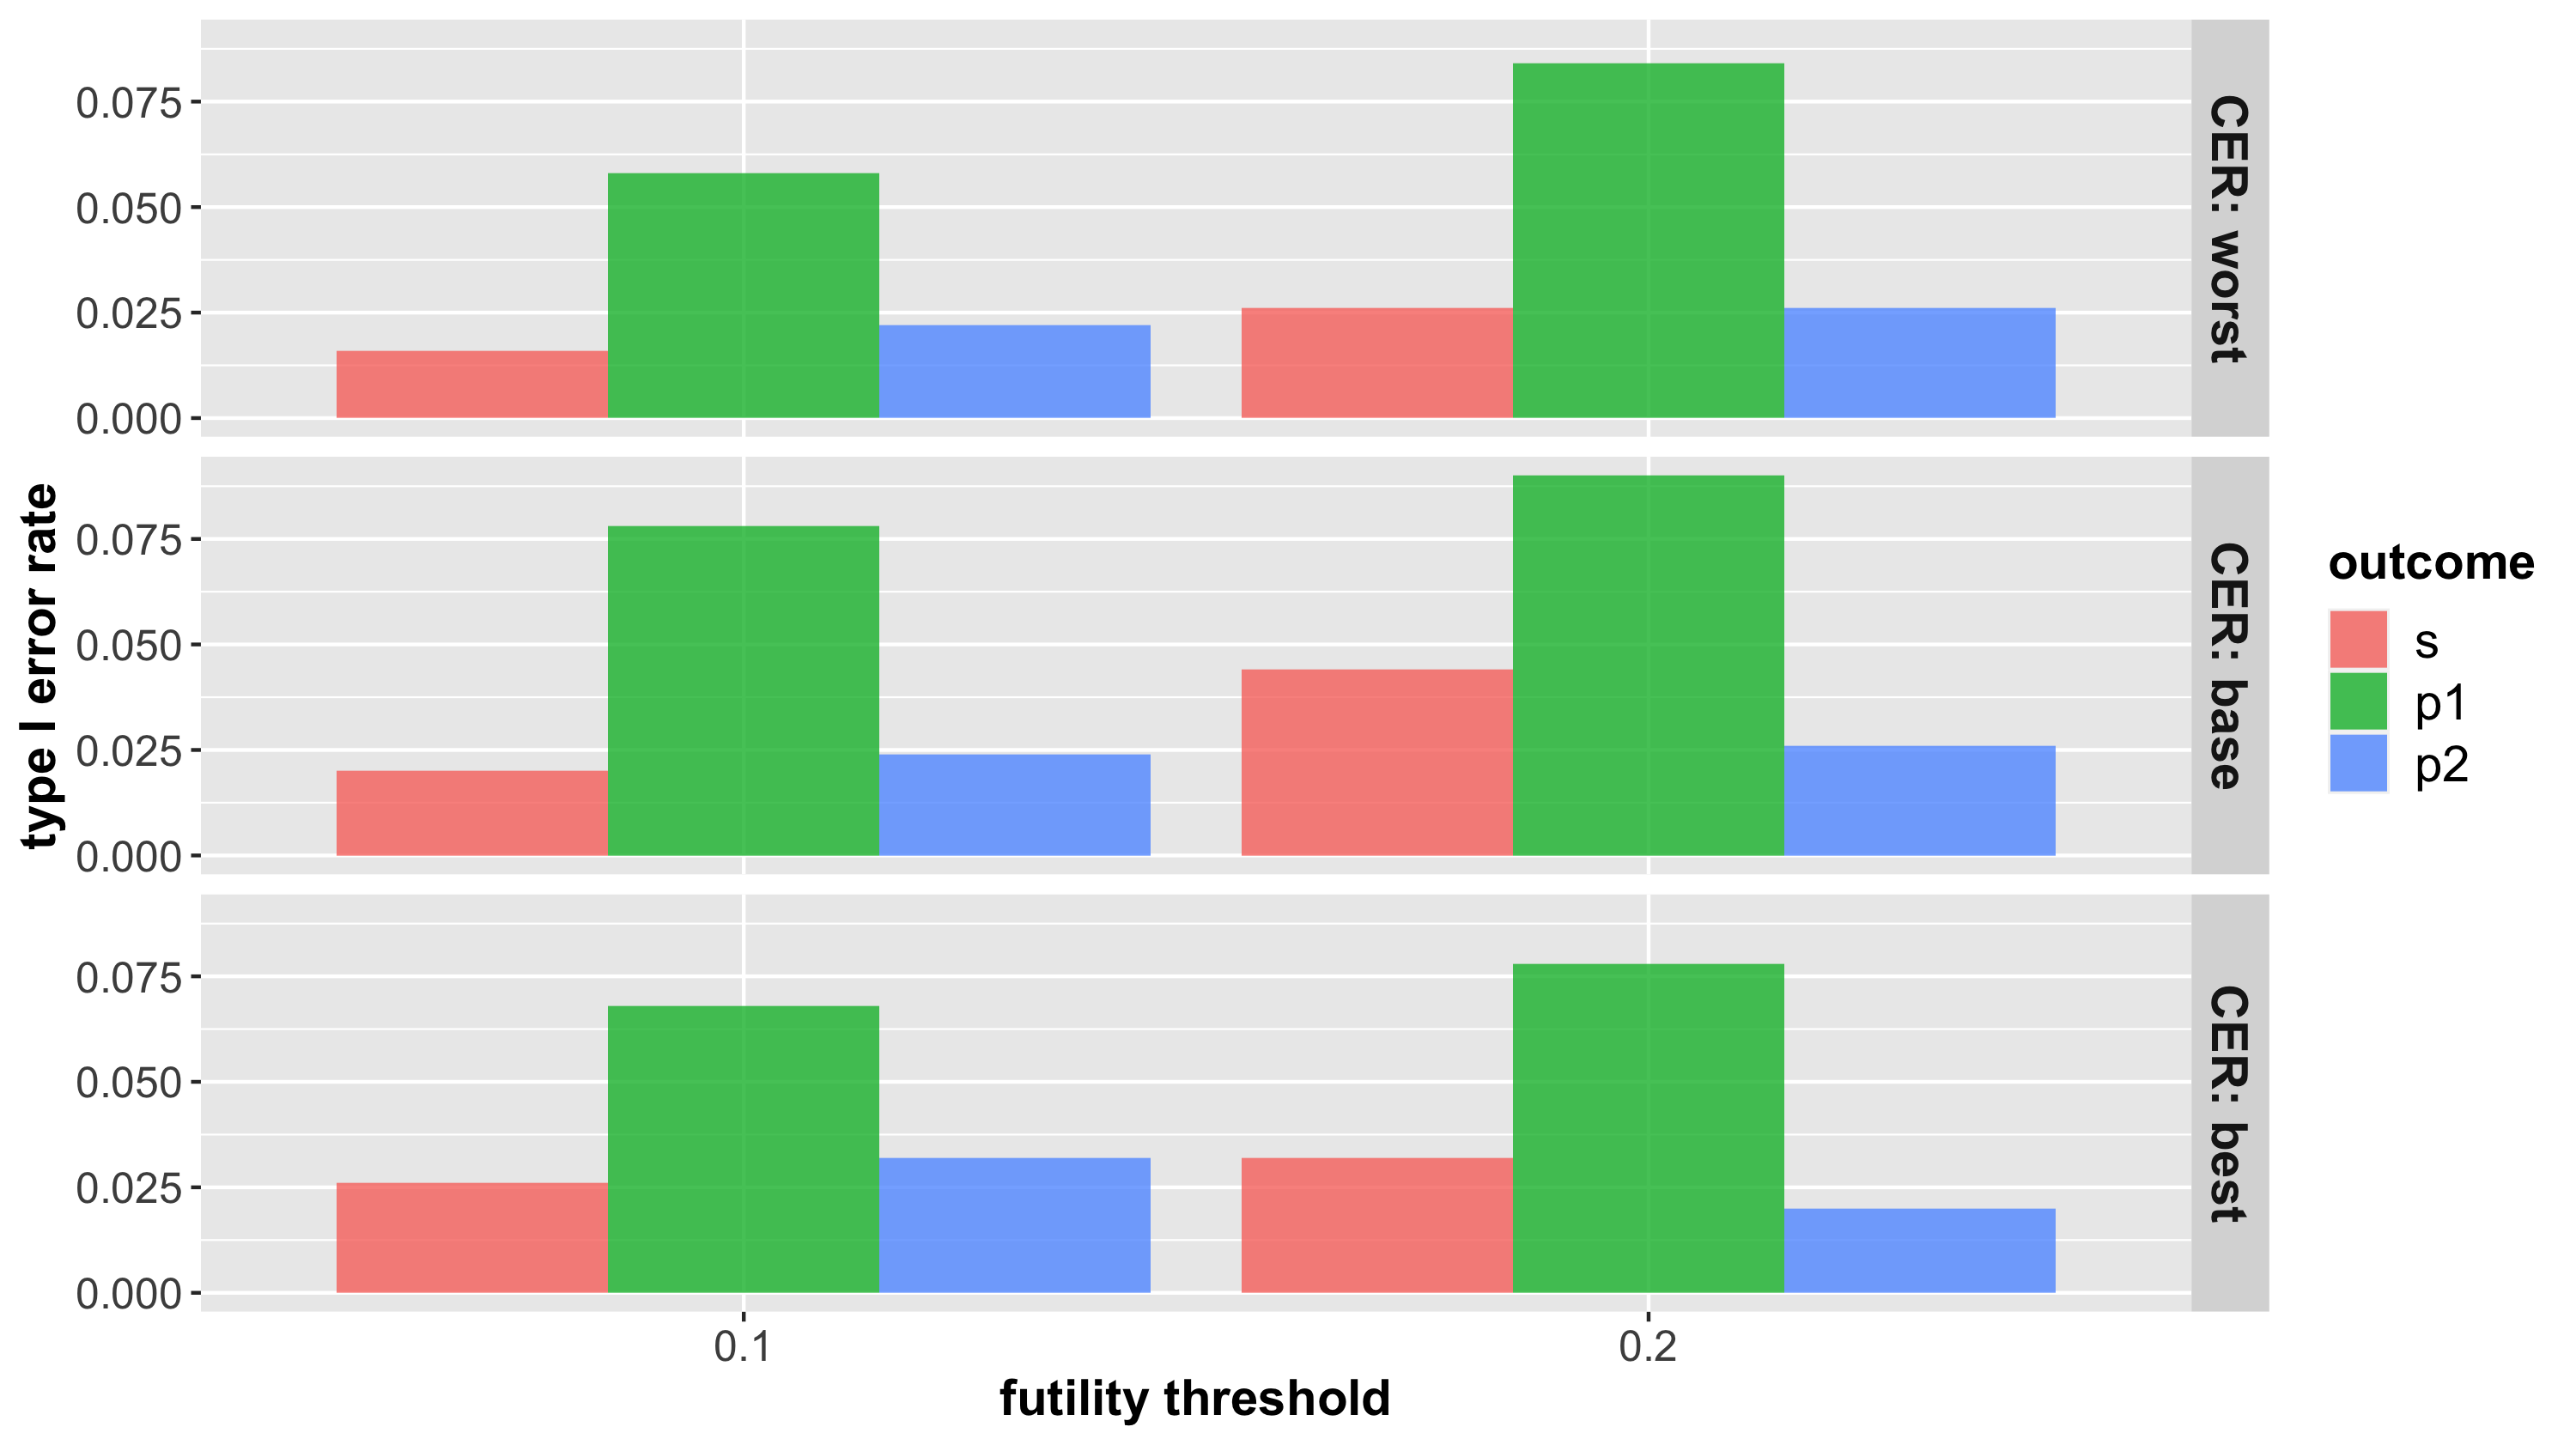
\includegraphics{../p1_plots/batch_size_nb_2000/type_1_error_p1.png}
\end{figure}

\hypertarget{power-1}{%
\subparagraph{Power}\label{power-1}}

\begin{figure}
  \caption{Power under the three relative risk reductions (RRR - upper column label) for each of the outcomes (lower column labels). 
  Power estimates by control event rates are presented by the rows. Power estimates by the futility thresholds are presented by the bar color (see legend).}
  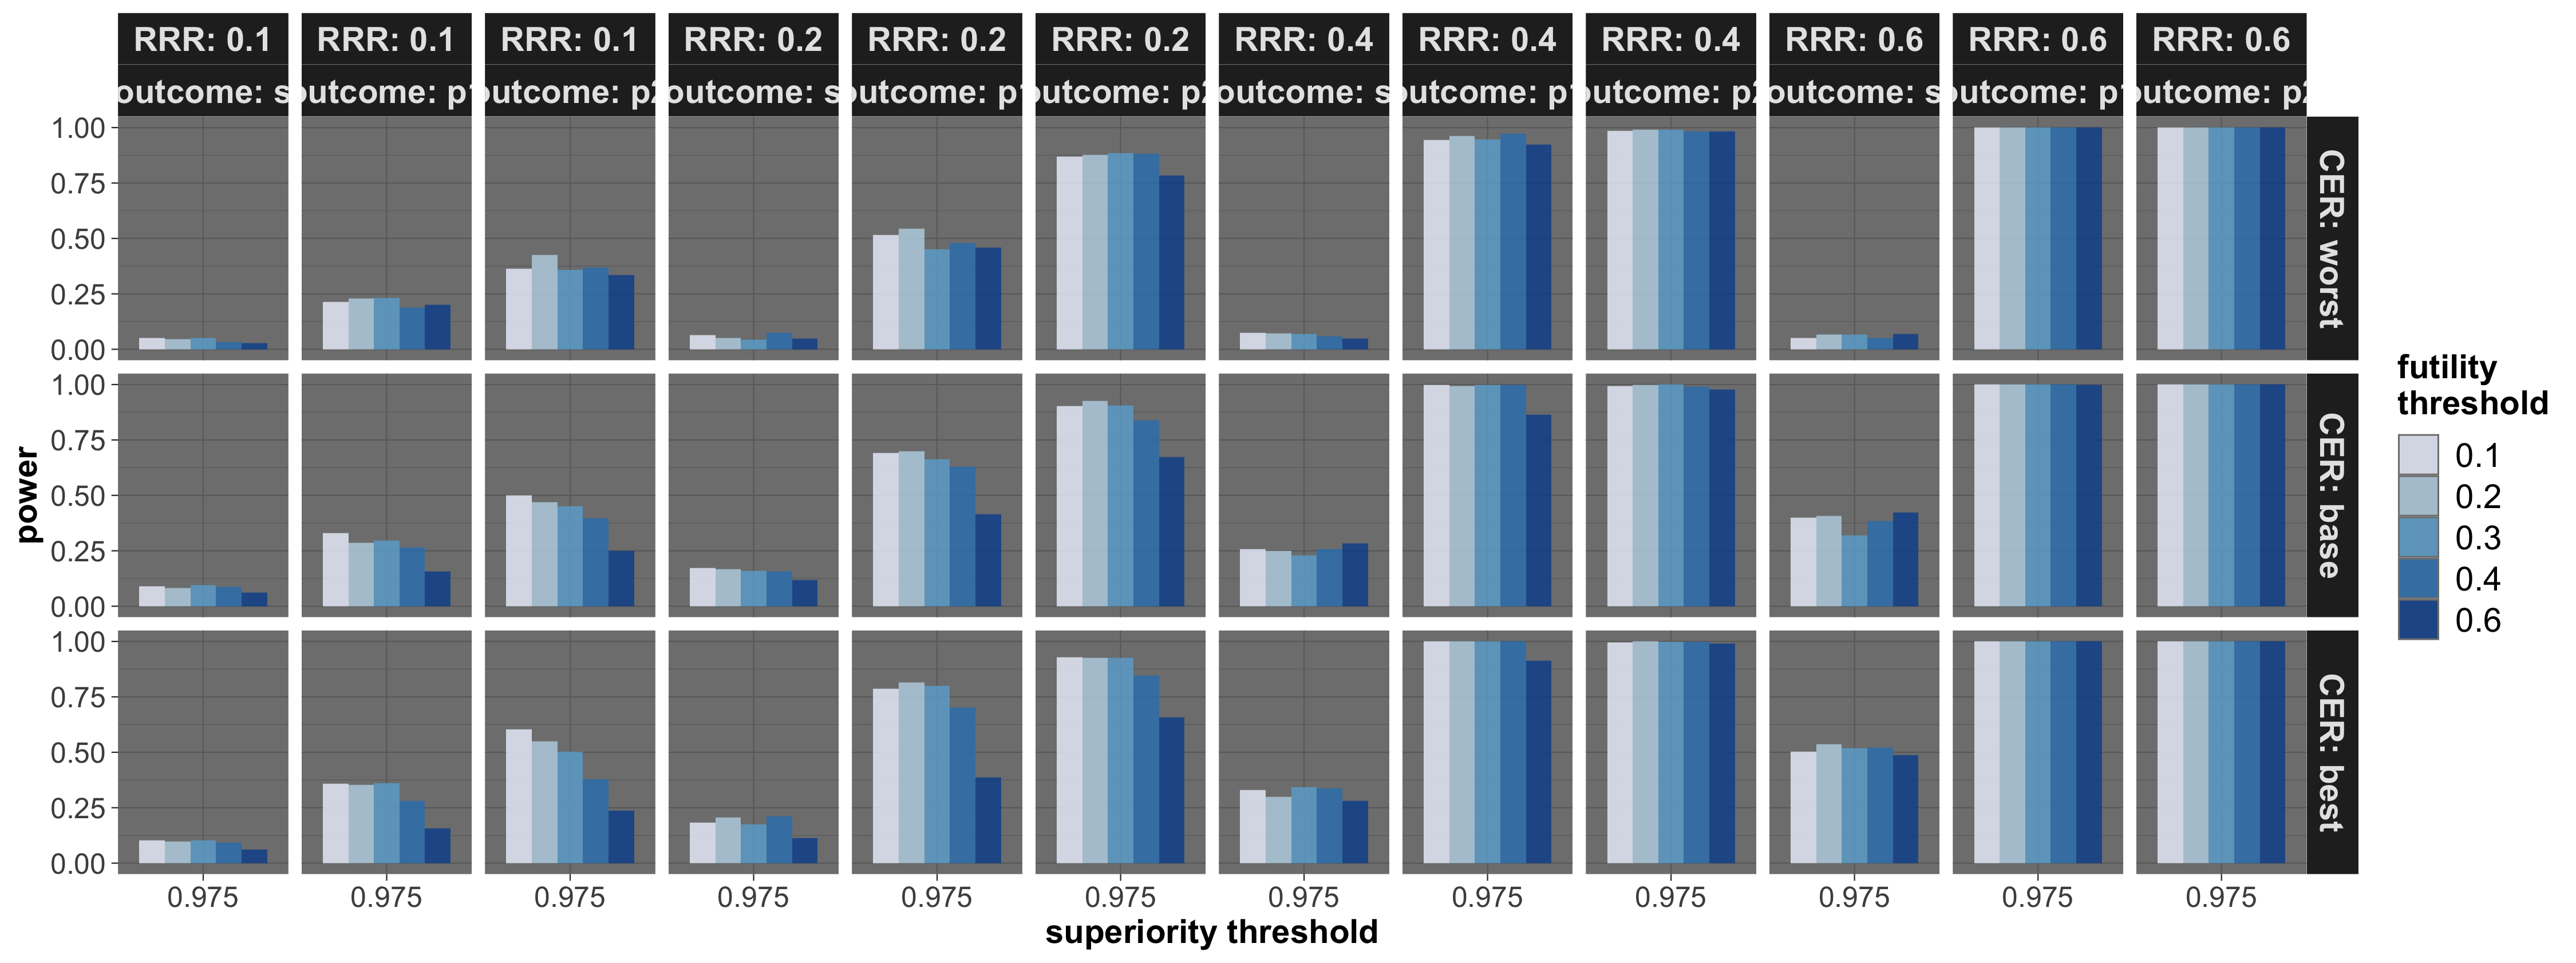
\includegraphics{../p1_plots/batch_size_nb_2000/power_all_p1.png}
\end{figure}

\begin{figure}
  \caption{Power under the three relative risk reductions (RRR - upper column label) for each of the outcomes (lower
  column labels or legend). Observed power for each outcome is presented by colored bars. Power estimates by control
  event rates are presented by the rows and correspond to a superiority threshold of 0.975.}
  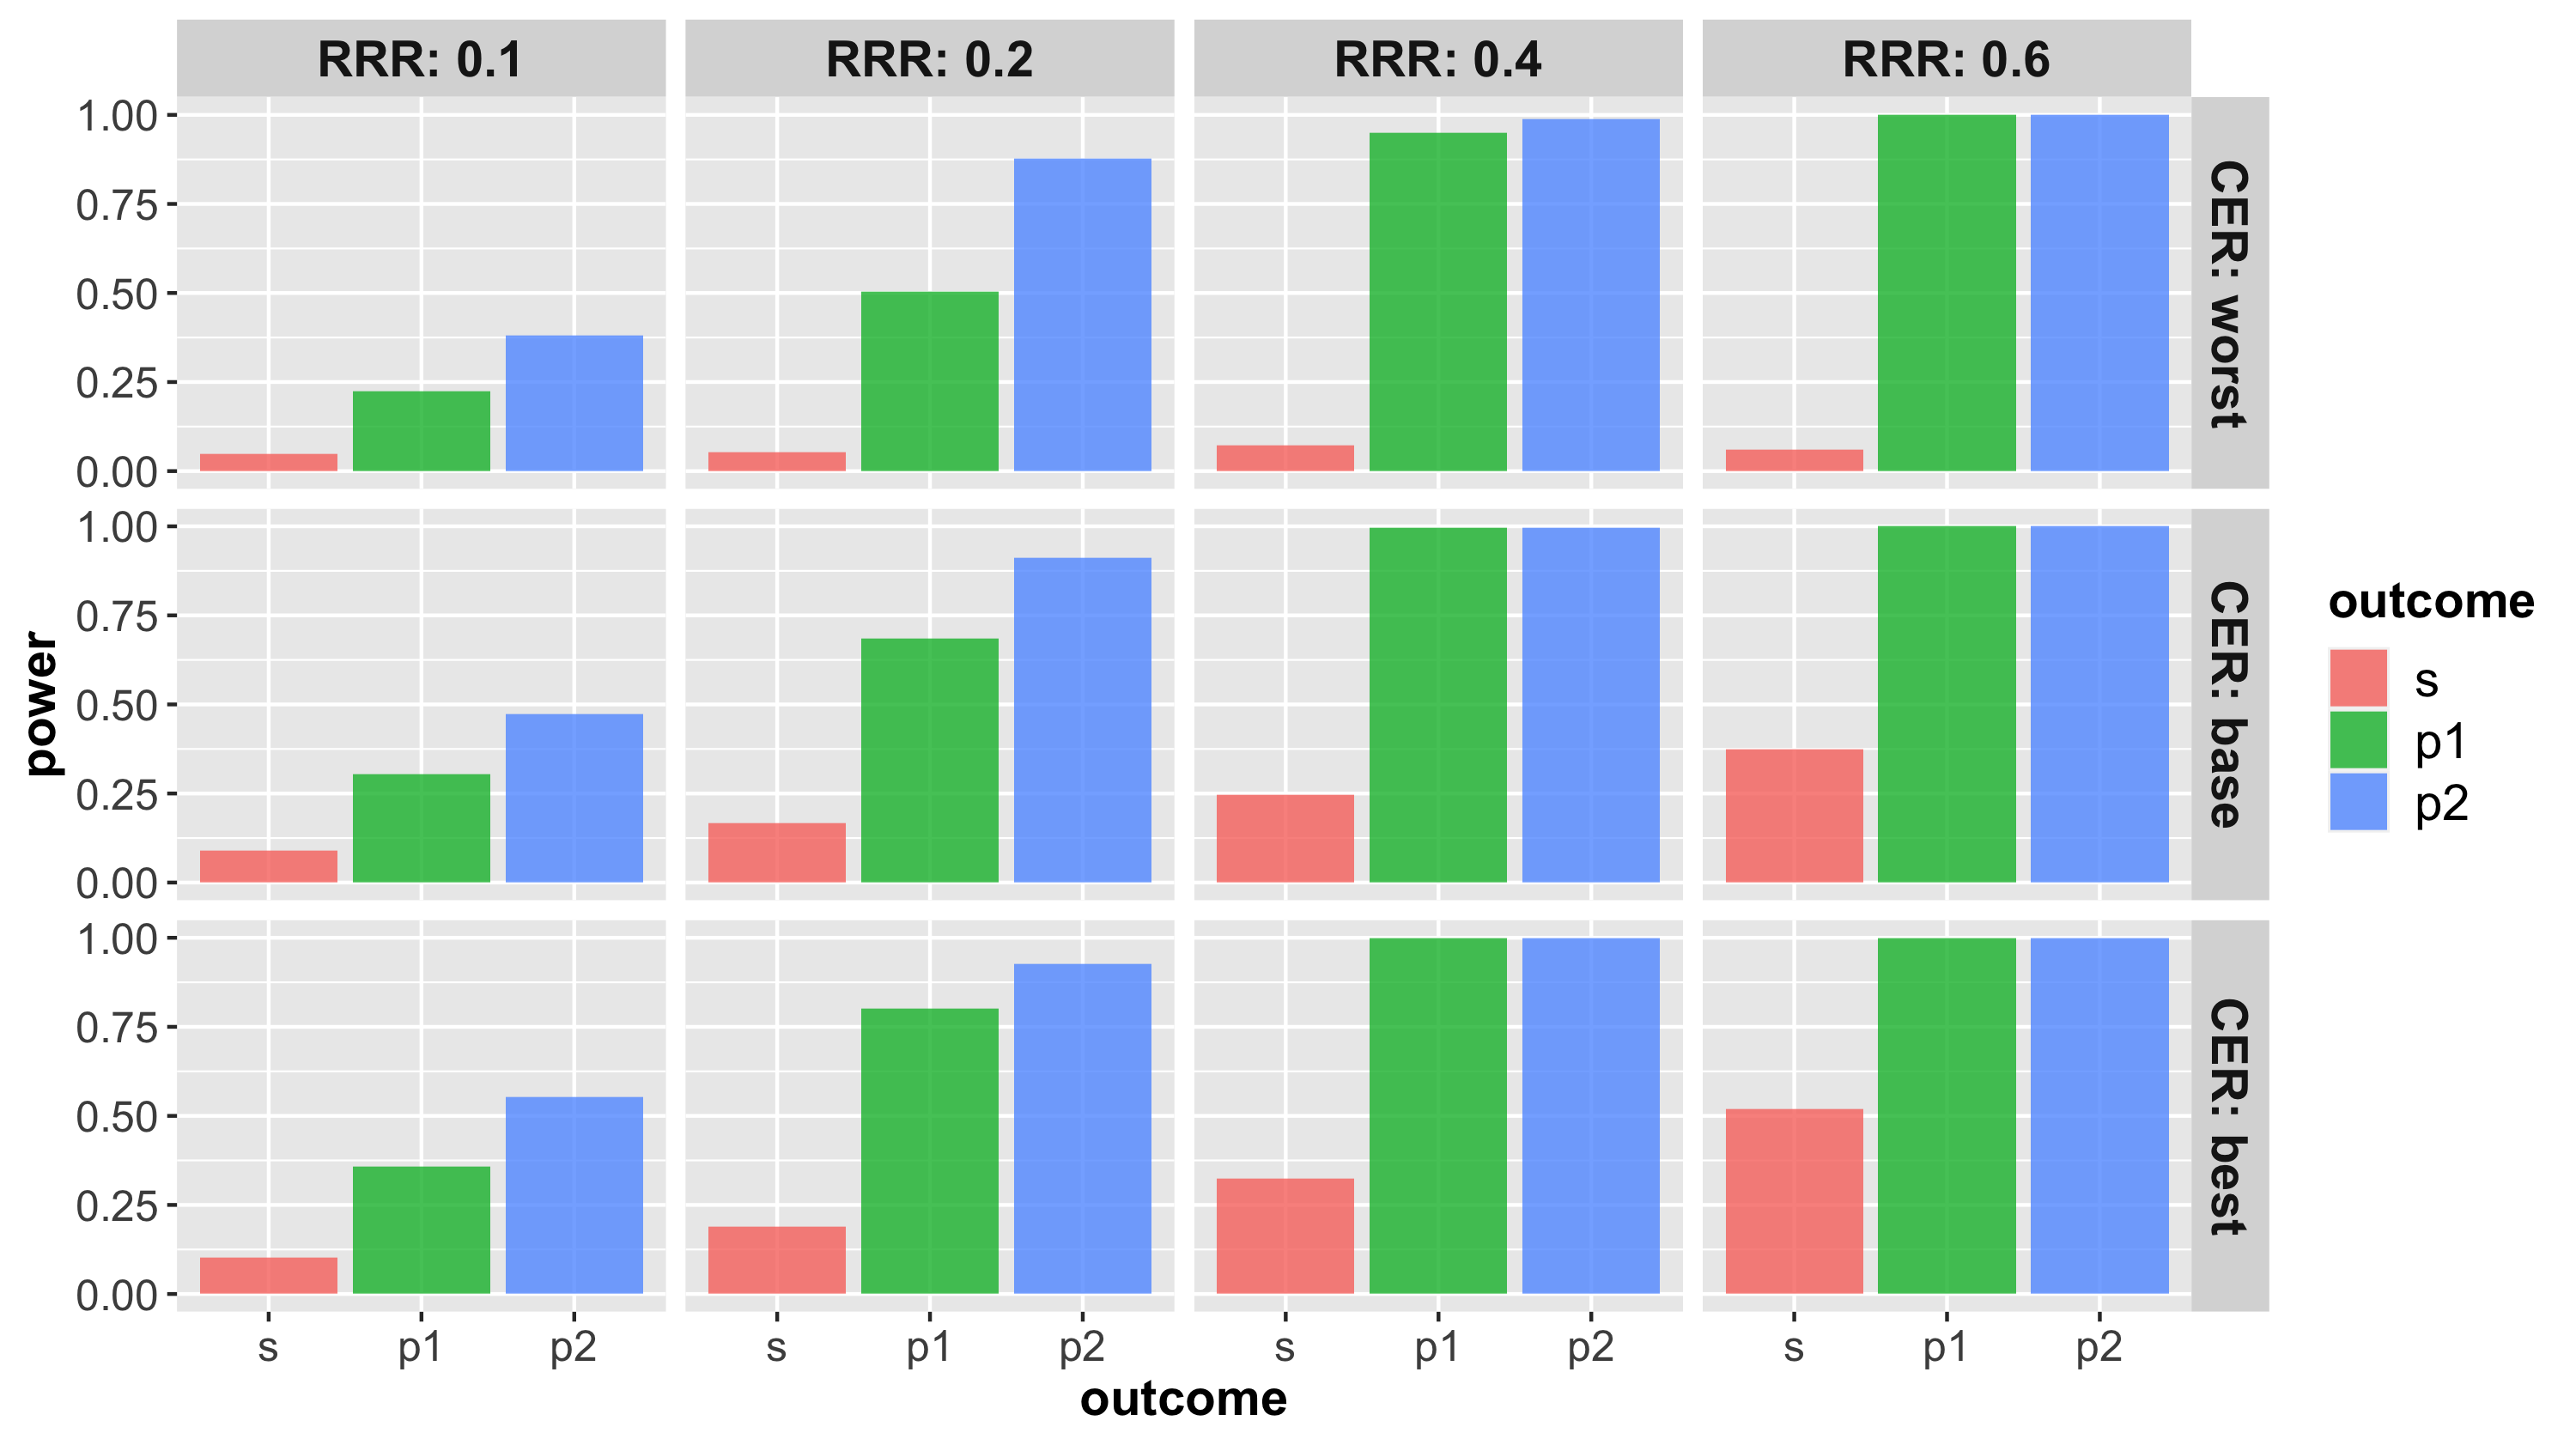
\includegraphics{../p1_plots/batch_size_nb_2000/power_p1.png}
\end{figure}

\hypertarget{expected-sample-size-1}{%
\subparagraph{Expected Sample Size}\label{expected-sample-size-1}}

\begin{figure}
  \caption{Expected sample size at trial termination. Results by control event scenarios are presented by rows. Results
  by relative risk reductions are presented by columns. Results by futility thresholds are presented by the color of the bars (see legend).}
  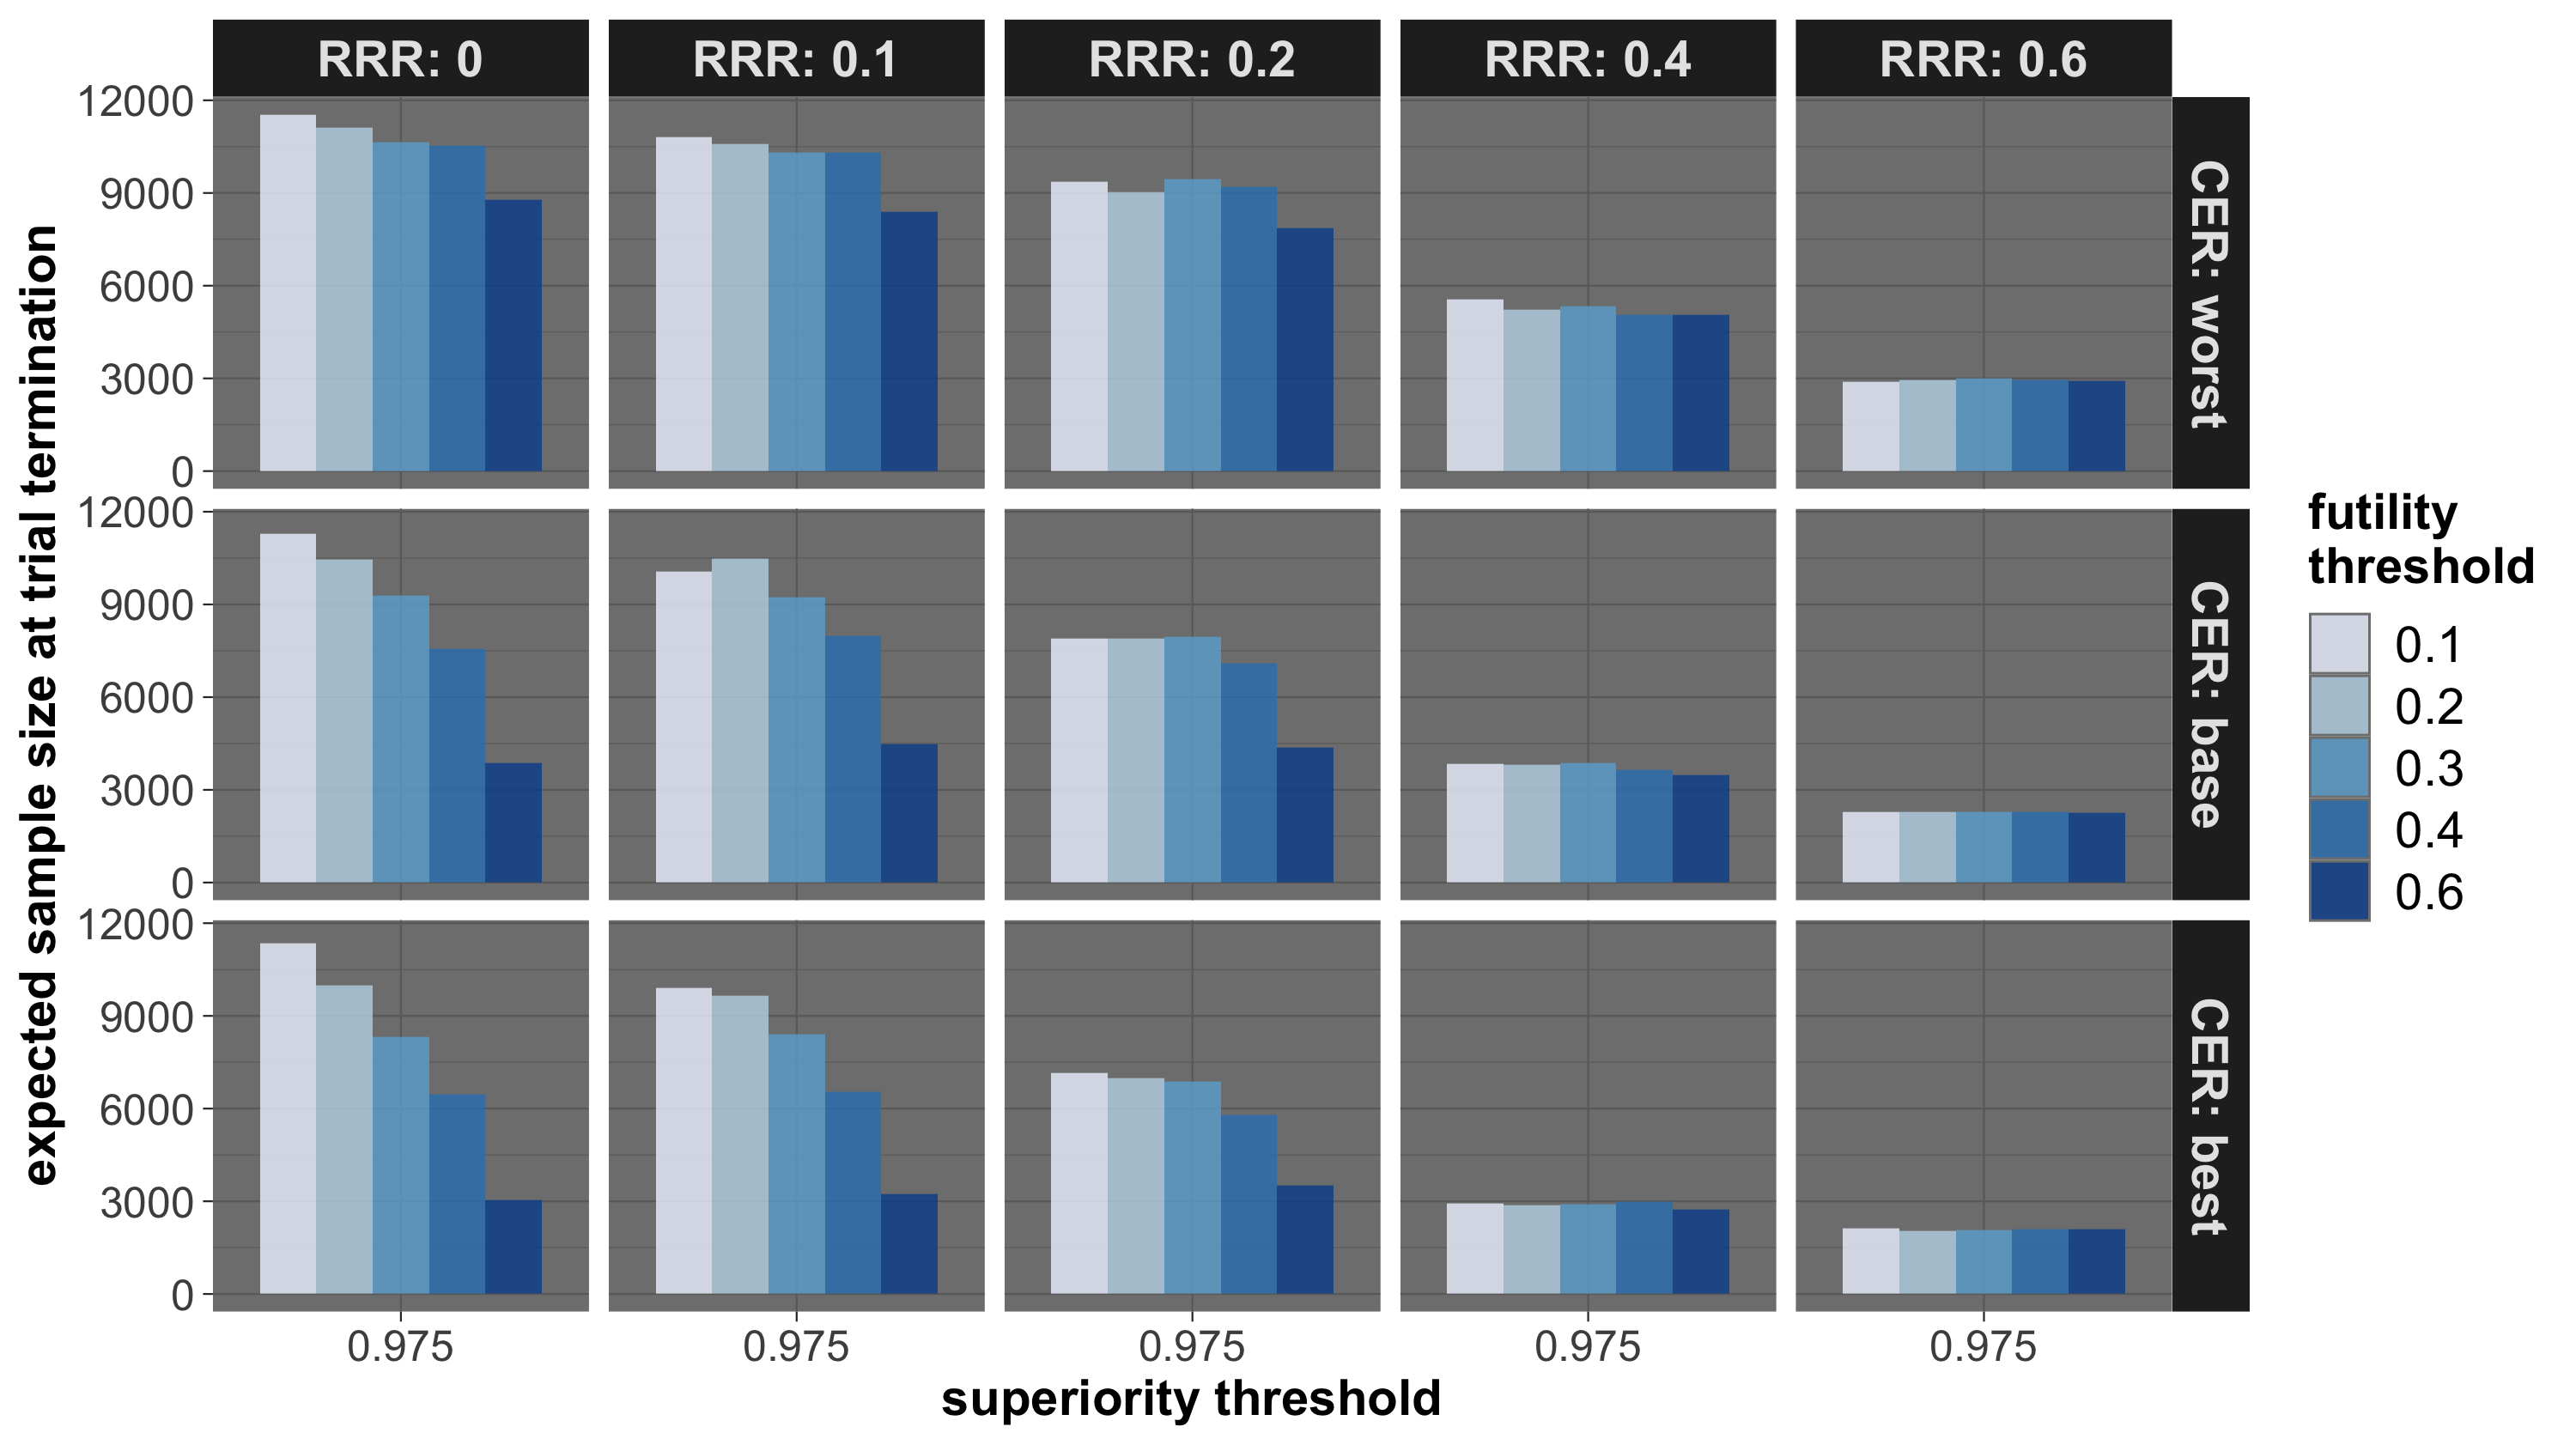
\includegraphics{../p1_plots/batch_size_nb_2000/exp_sample_size_p1.png}
\end{figure}

\hypertarget{probability-of-reaching-maximum-sample-size-1}{%
\paragraph{Probability of Reaching Maximum Sample
Size}\label{probability-of-reaching-maximum-sample-size-1}}

\begin{figure}
  \caption{Probability of reaching maximum sample size for the three control event rates (CER – rows), four relative
  risk reductions (RRR – columns), and three futility thresholds (legend).}
  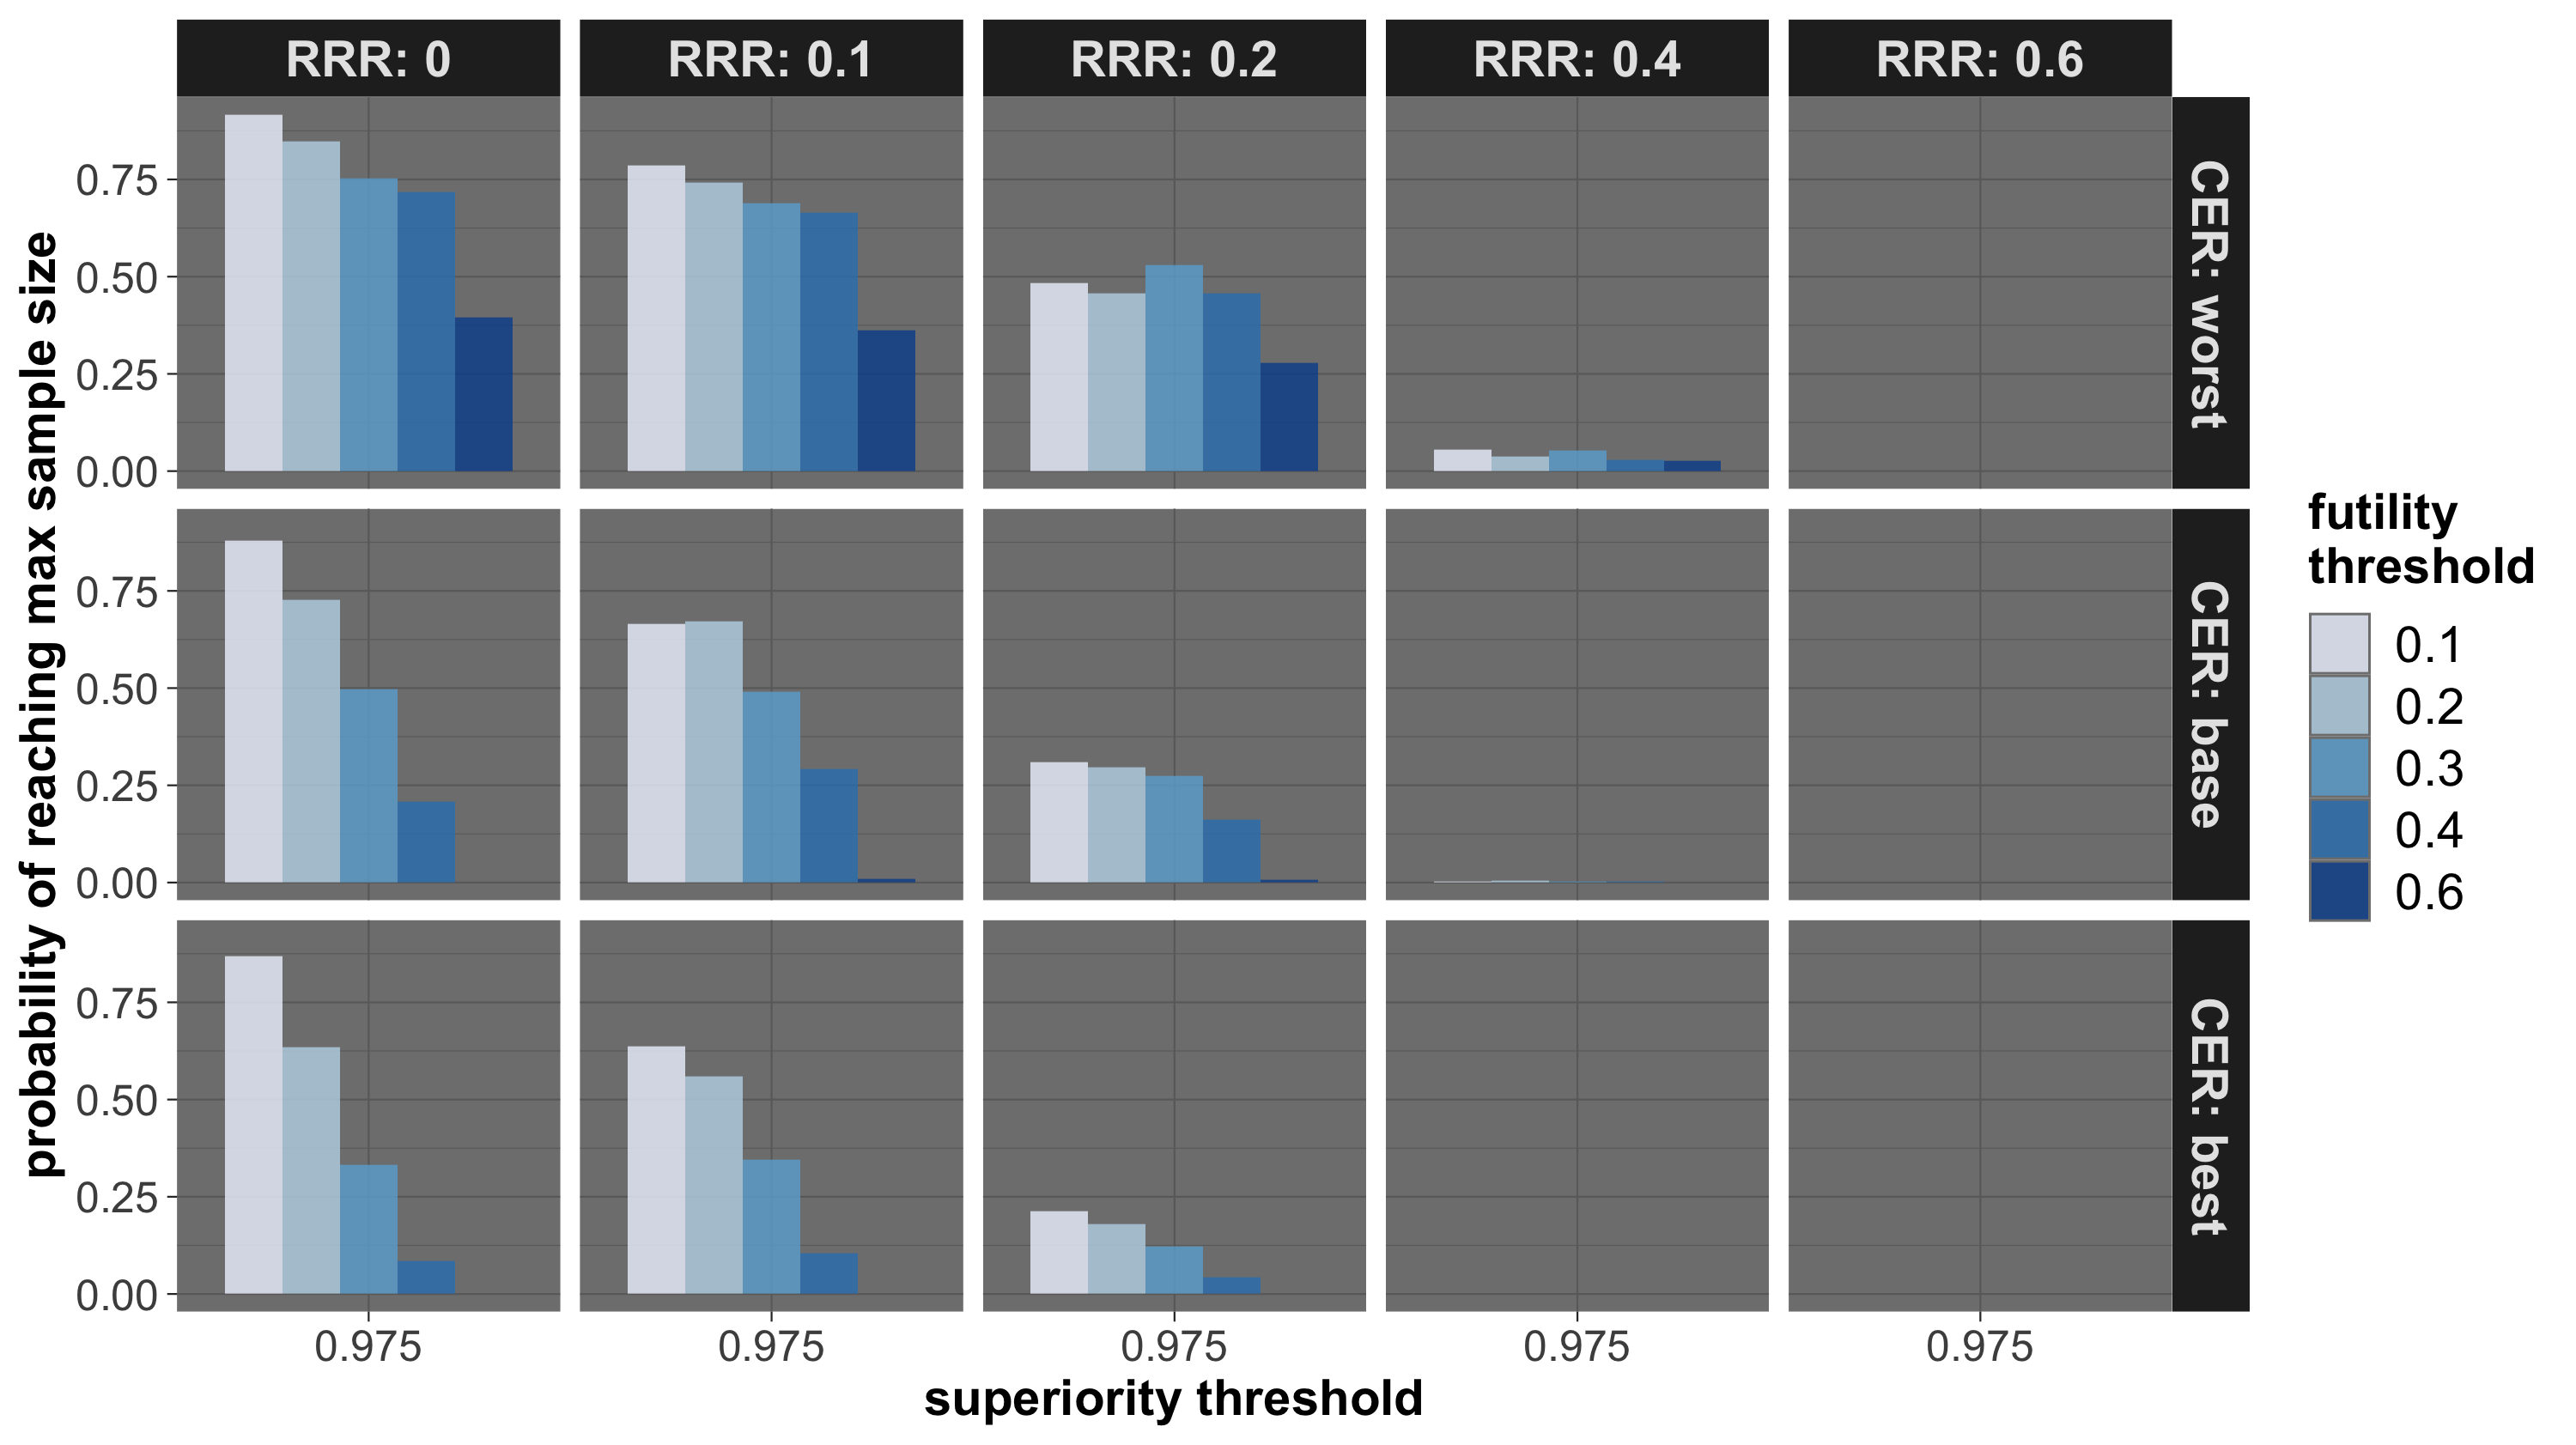
\includegraphics{../p1_plots/batch_size_nb_2000/prob_reach_max_size_p1.png}
\end{figure}

\hypertarget{probability-of-stopping-early-1}{%
\paragraph{Probability of Stopping
Early}\label{probability-of-stopping-early-1}}

\begin{figure}
  \caption{Probability of stopping early due to futility or superiority for the three control event rates (CER – rows),
  four relative risk reductions (RRR – columns), three superiority thresholds (x axis) and three futility thresholds
  (legend).}
  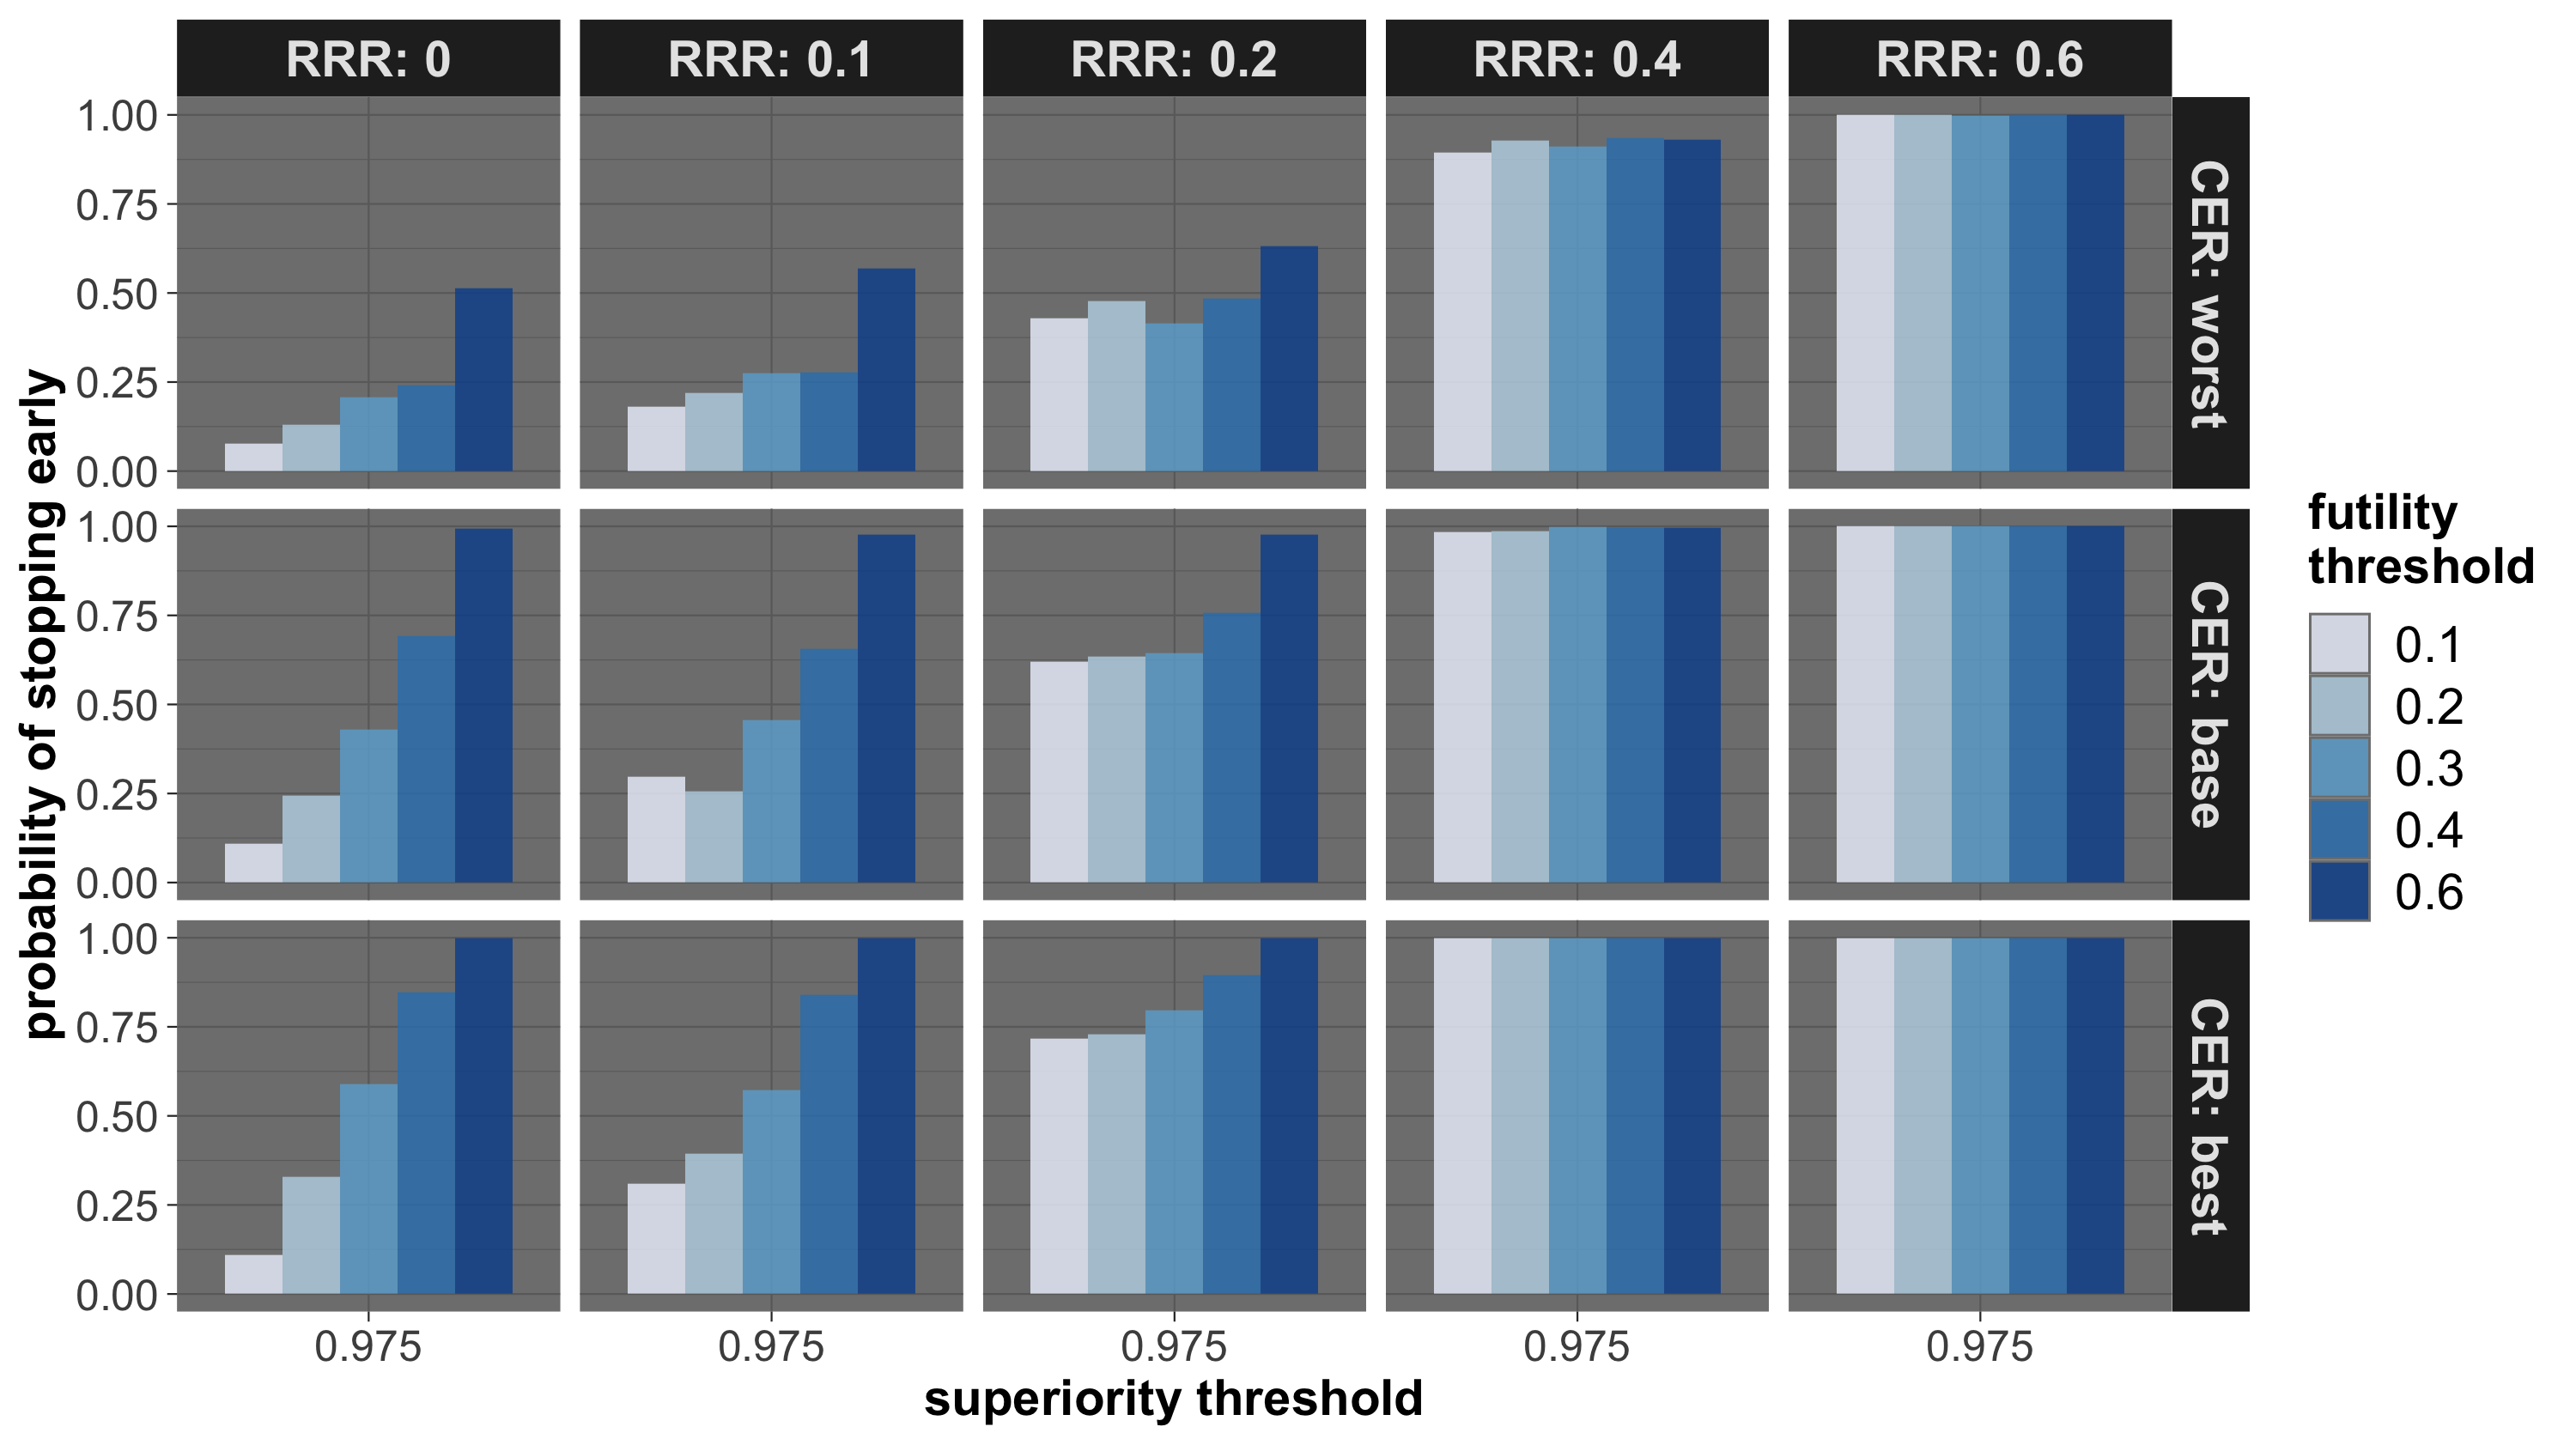
\includegraphics{../p1_plots/batch_size_nb_2000/prob_stop_early_p1.png}
\end{figure}

\begin{figure}
\centering
  \caption{Probability of stopping early due to futility, and stopping early due to superiority. Stopping probabilities
  are presented for the three control event rates (CER – rows), four relative risk reductions (RRR – columns), and three futility thresholds (legend).}
  \label{fig:fig}
  \begin{subfigure}{0.8\textwidth}
    \centering
    \caption{}
    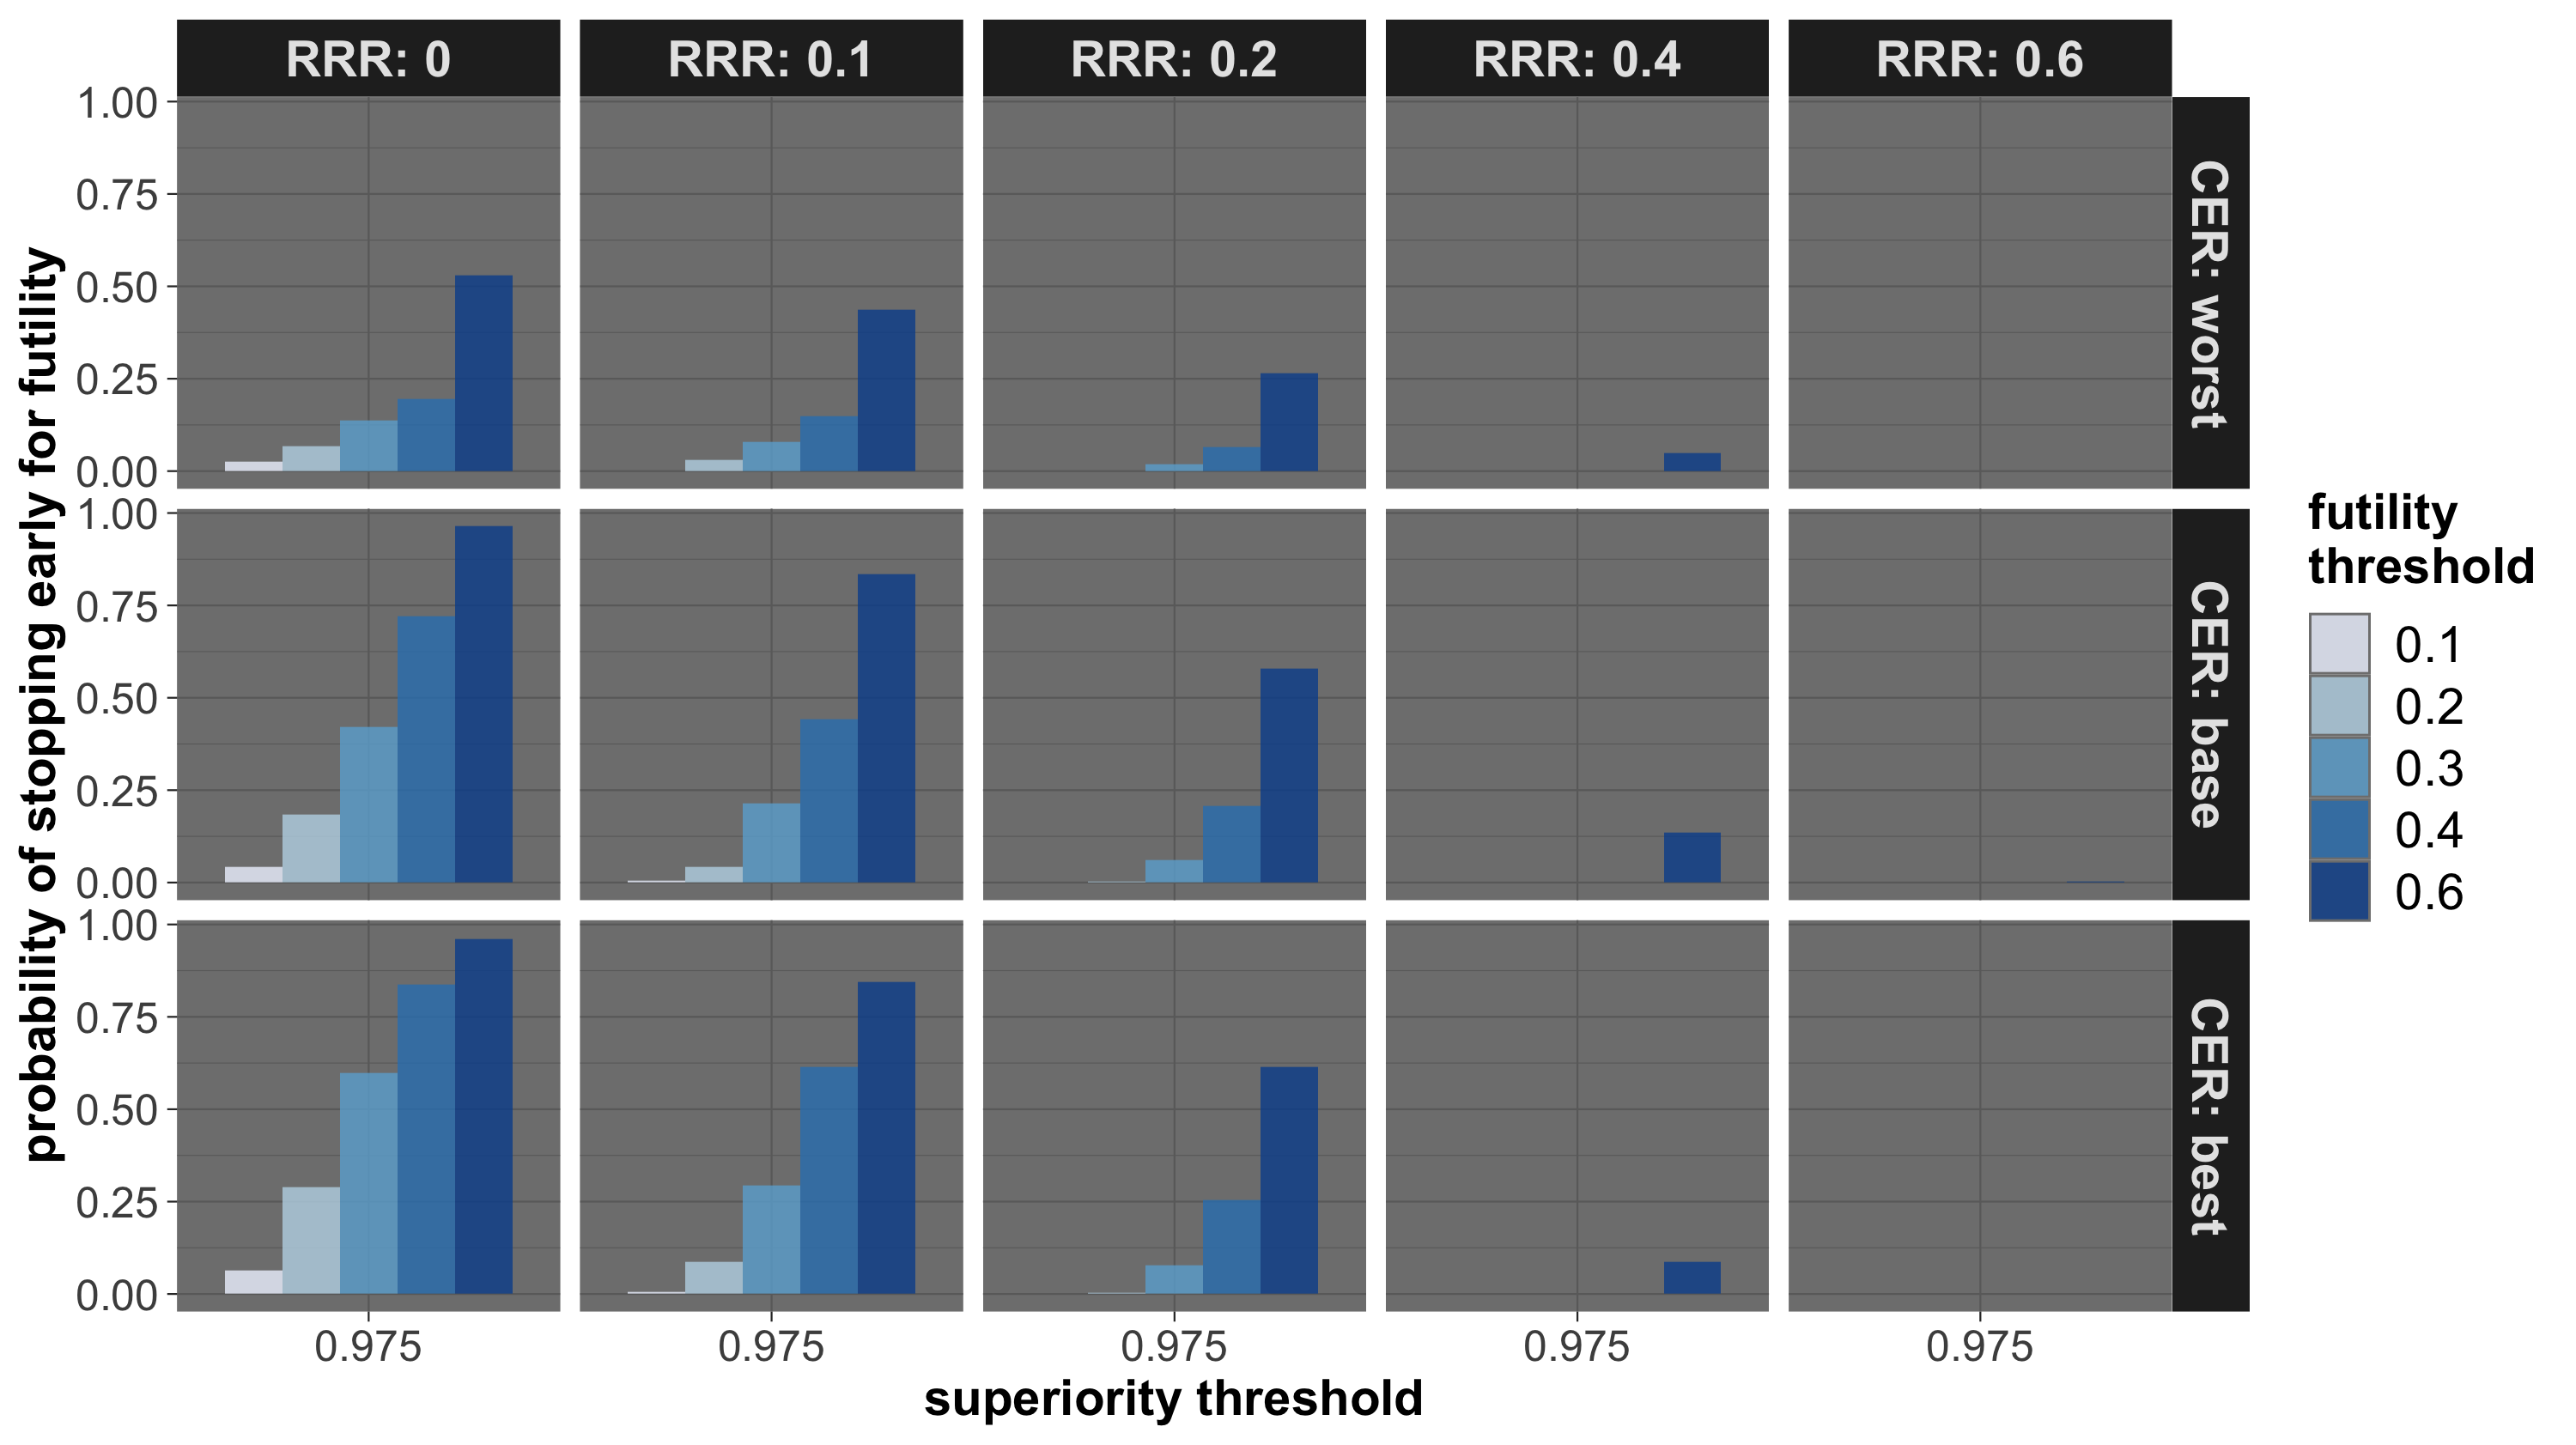
\includegraphics{../p1_plots/batch_size_nb_2000/prob_stop_early_fut_p1.png}
  \end{subfigure}
  \begin{subfigure}{0.8\textwidth}
    \centering
    \caption{}
    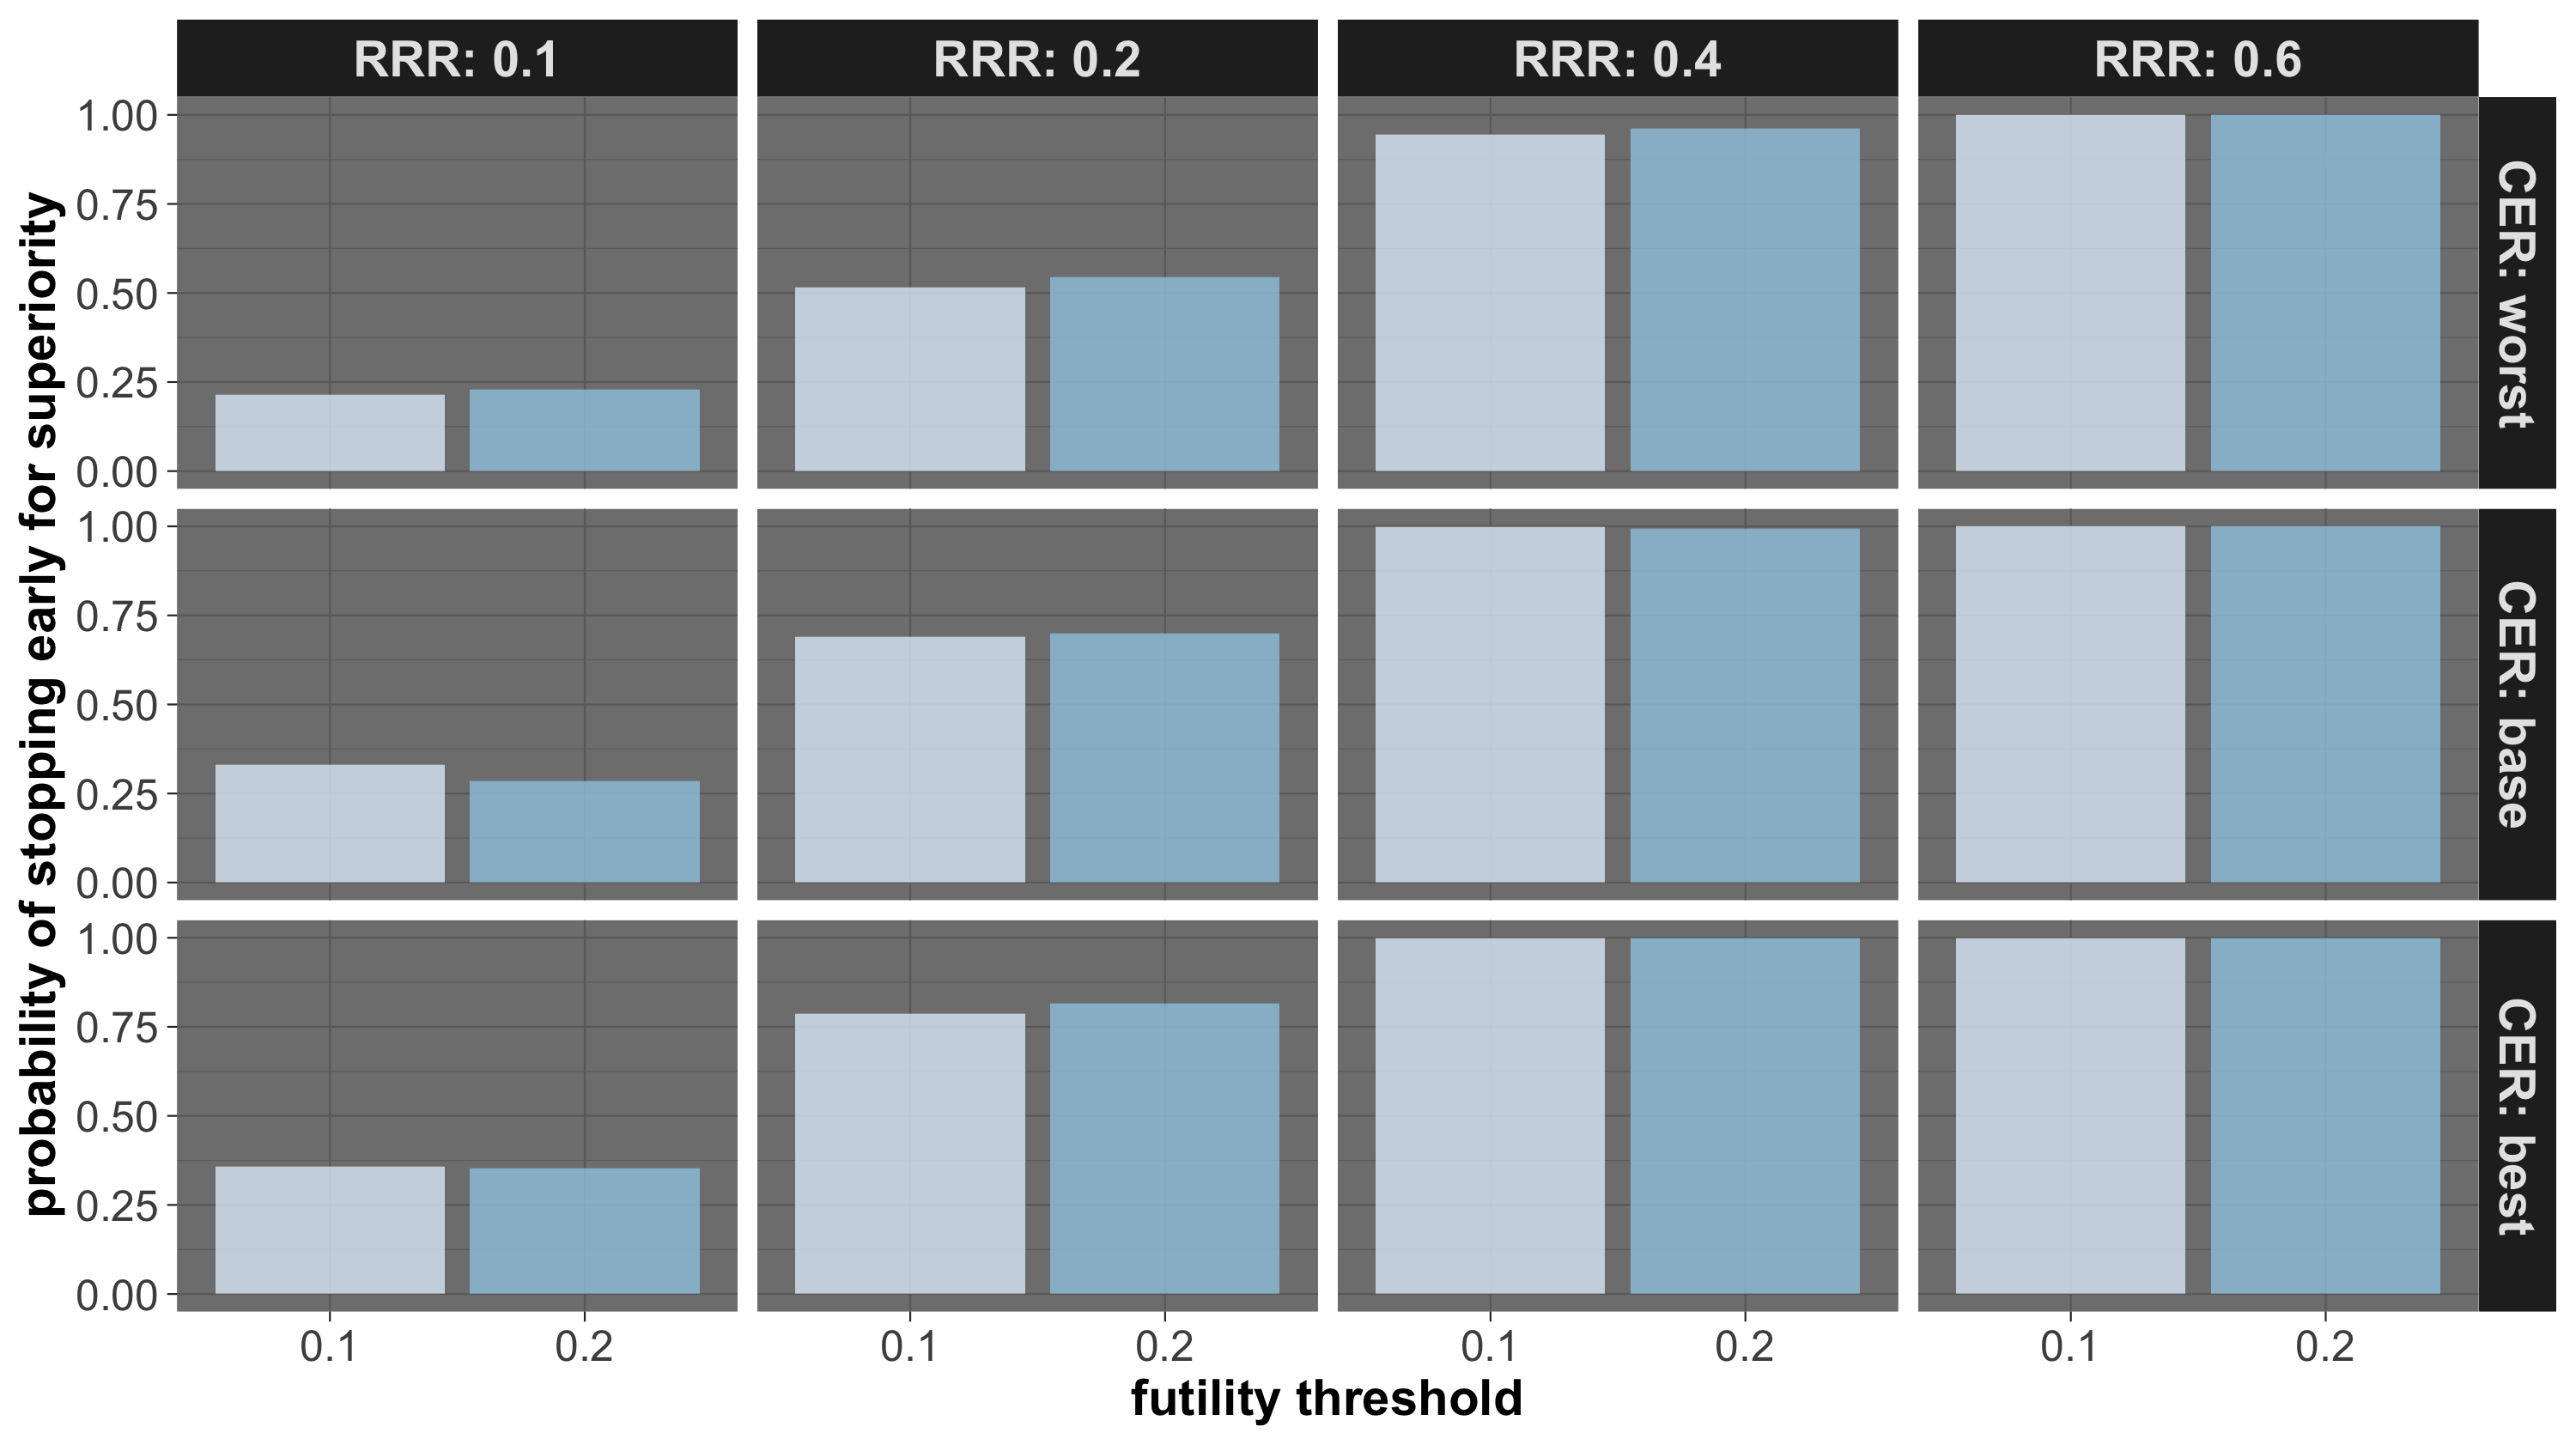
\includegraphics{../p1_plots/batch_size_nb_2000/prob_stop_early_sup_p1.png}
  \end{subfigure}
\end{figure}

\hypertarget{p-values-at-trial-termination-when-a-true-effect-exists-1}{%
\paragraph{P-values at trial termination when a true effect
exists}\label{p-values-at-trial-termination-when-a-true-effect-exists-1}}

\begin{figure}
  \caption{Overall probability at trial termination that the p-value (from Fisher’s exact test) at termination of the
  trial is below 5\%, between 5\% and 10\% and greater than 10\%. The rows represent the three control even rate scenarios
  and the three columns present the three relative risk reduction scenarios.}
  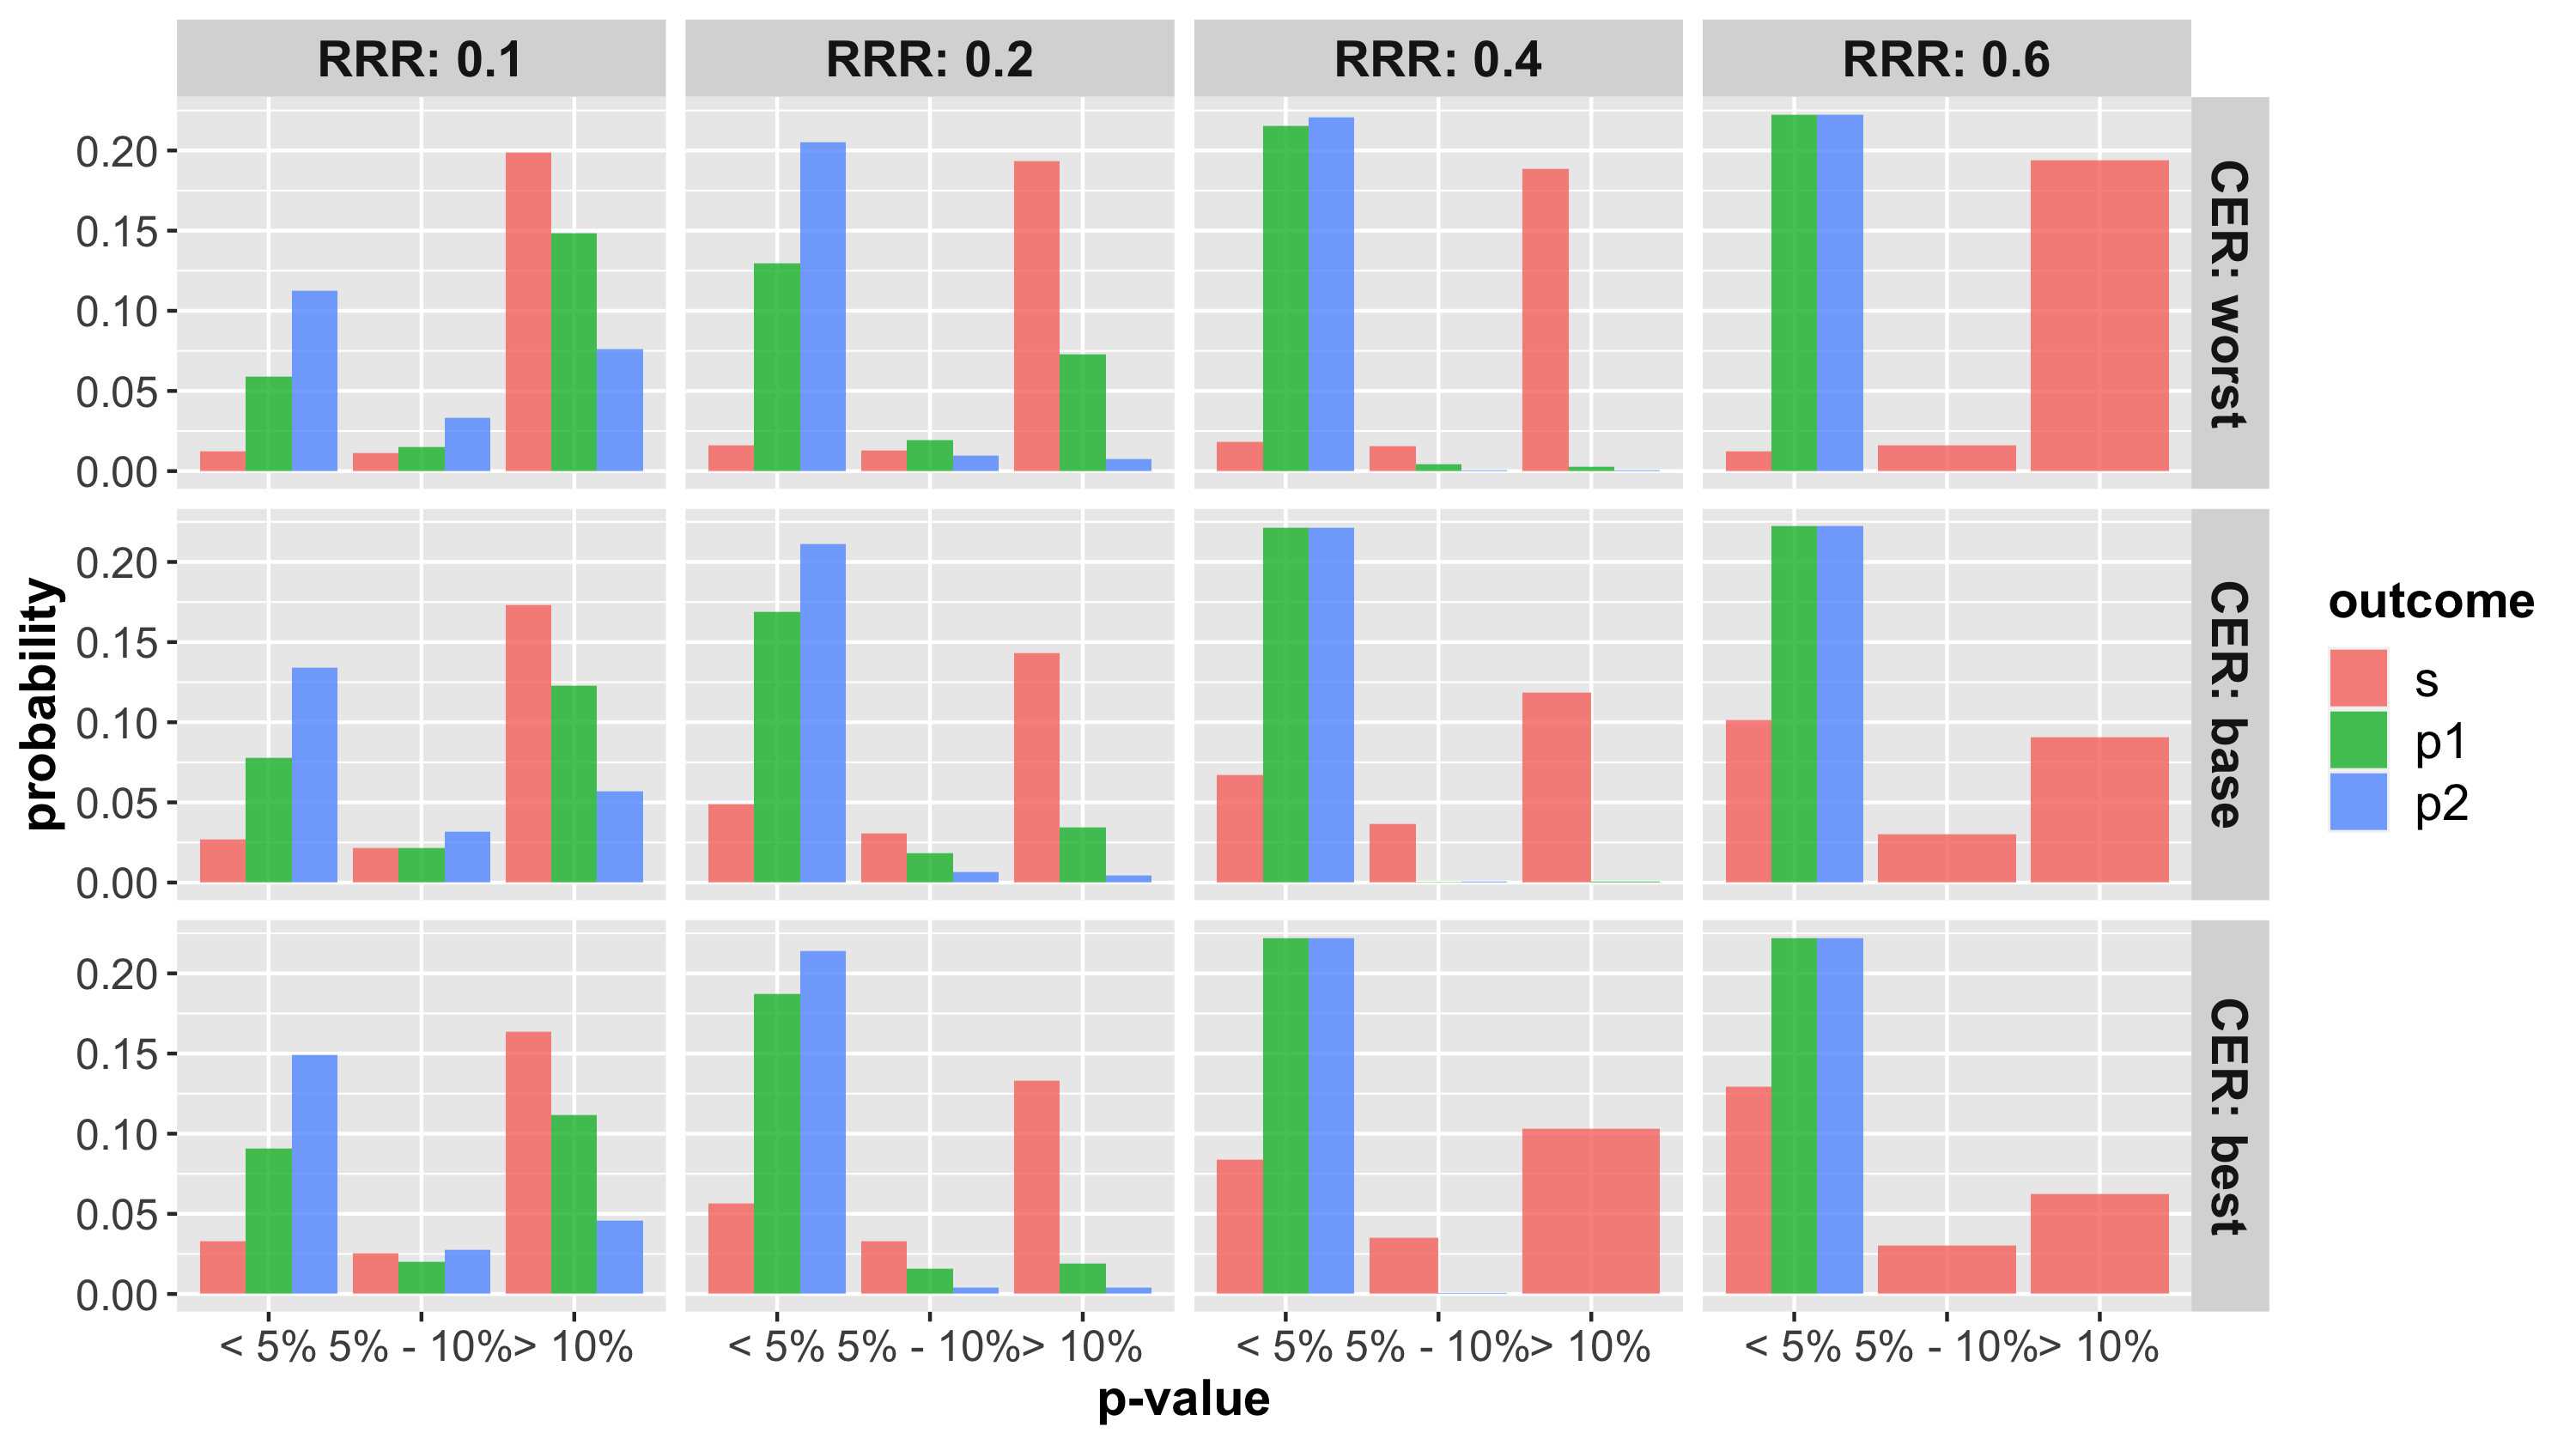
\includegraphics{../p1_plots/batch_size_nb_2000/pvalue_p1.png}
\end{figure}

\begin{figure}
\centering
  \caption{Probability that the p-value (from Fisher’s exact test) at termination of the trial is below 5\%, between 5\%
  and 10\% and greater than 10\% for cases where trial was (a) stopped for futility; (b) stopped for superiority. The
  rows represent the three control even rate scenarios and the three columns present the three relative risk reduction
  scenarios. Note: the denominator in each figure is the number of simulations (not the number of trials stopped for
  futility (a) or superiority (b), and thus, the proportions do not add up to 100\% within one figure. Further, (a) and
  (b) do not include simulations where the trial went to the max. allowed sample size. The bars should be interpreted
  with respect to the relative proportion that fit in each category.}
  \begin{subfigure}{0.8\textwidth}
    \centering
    \caption{}
    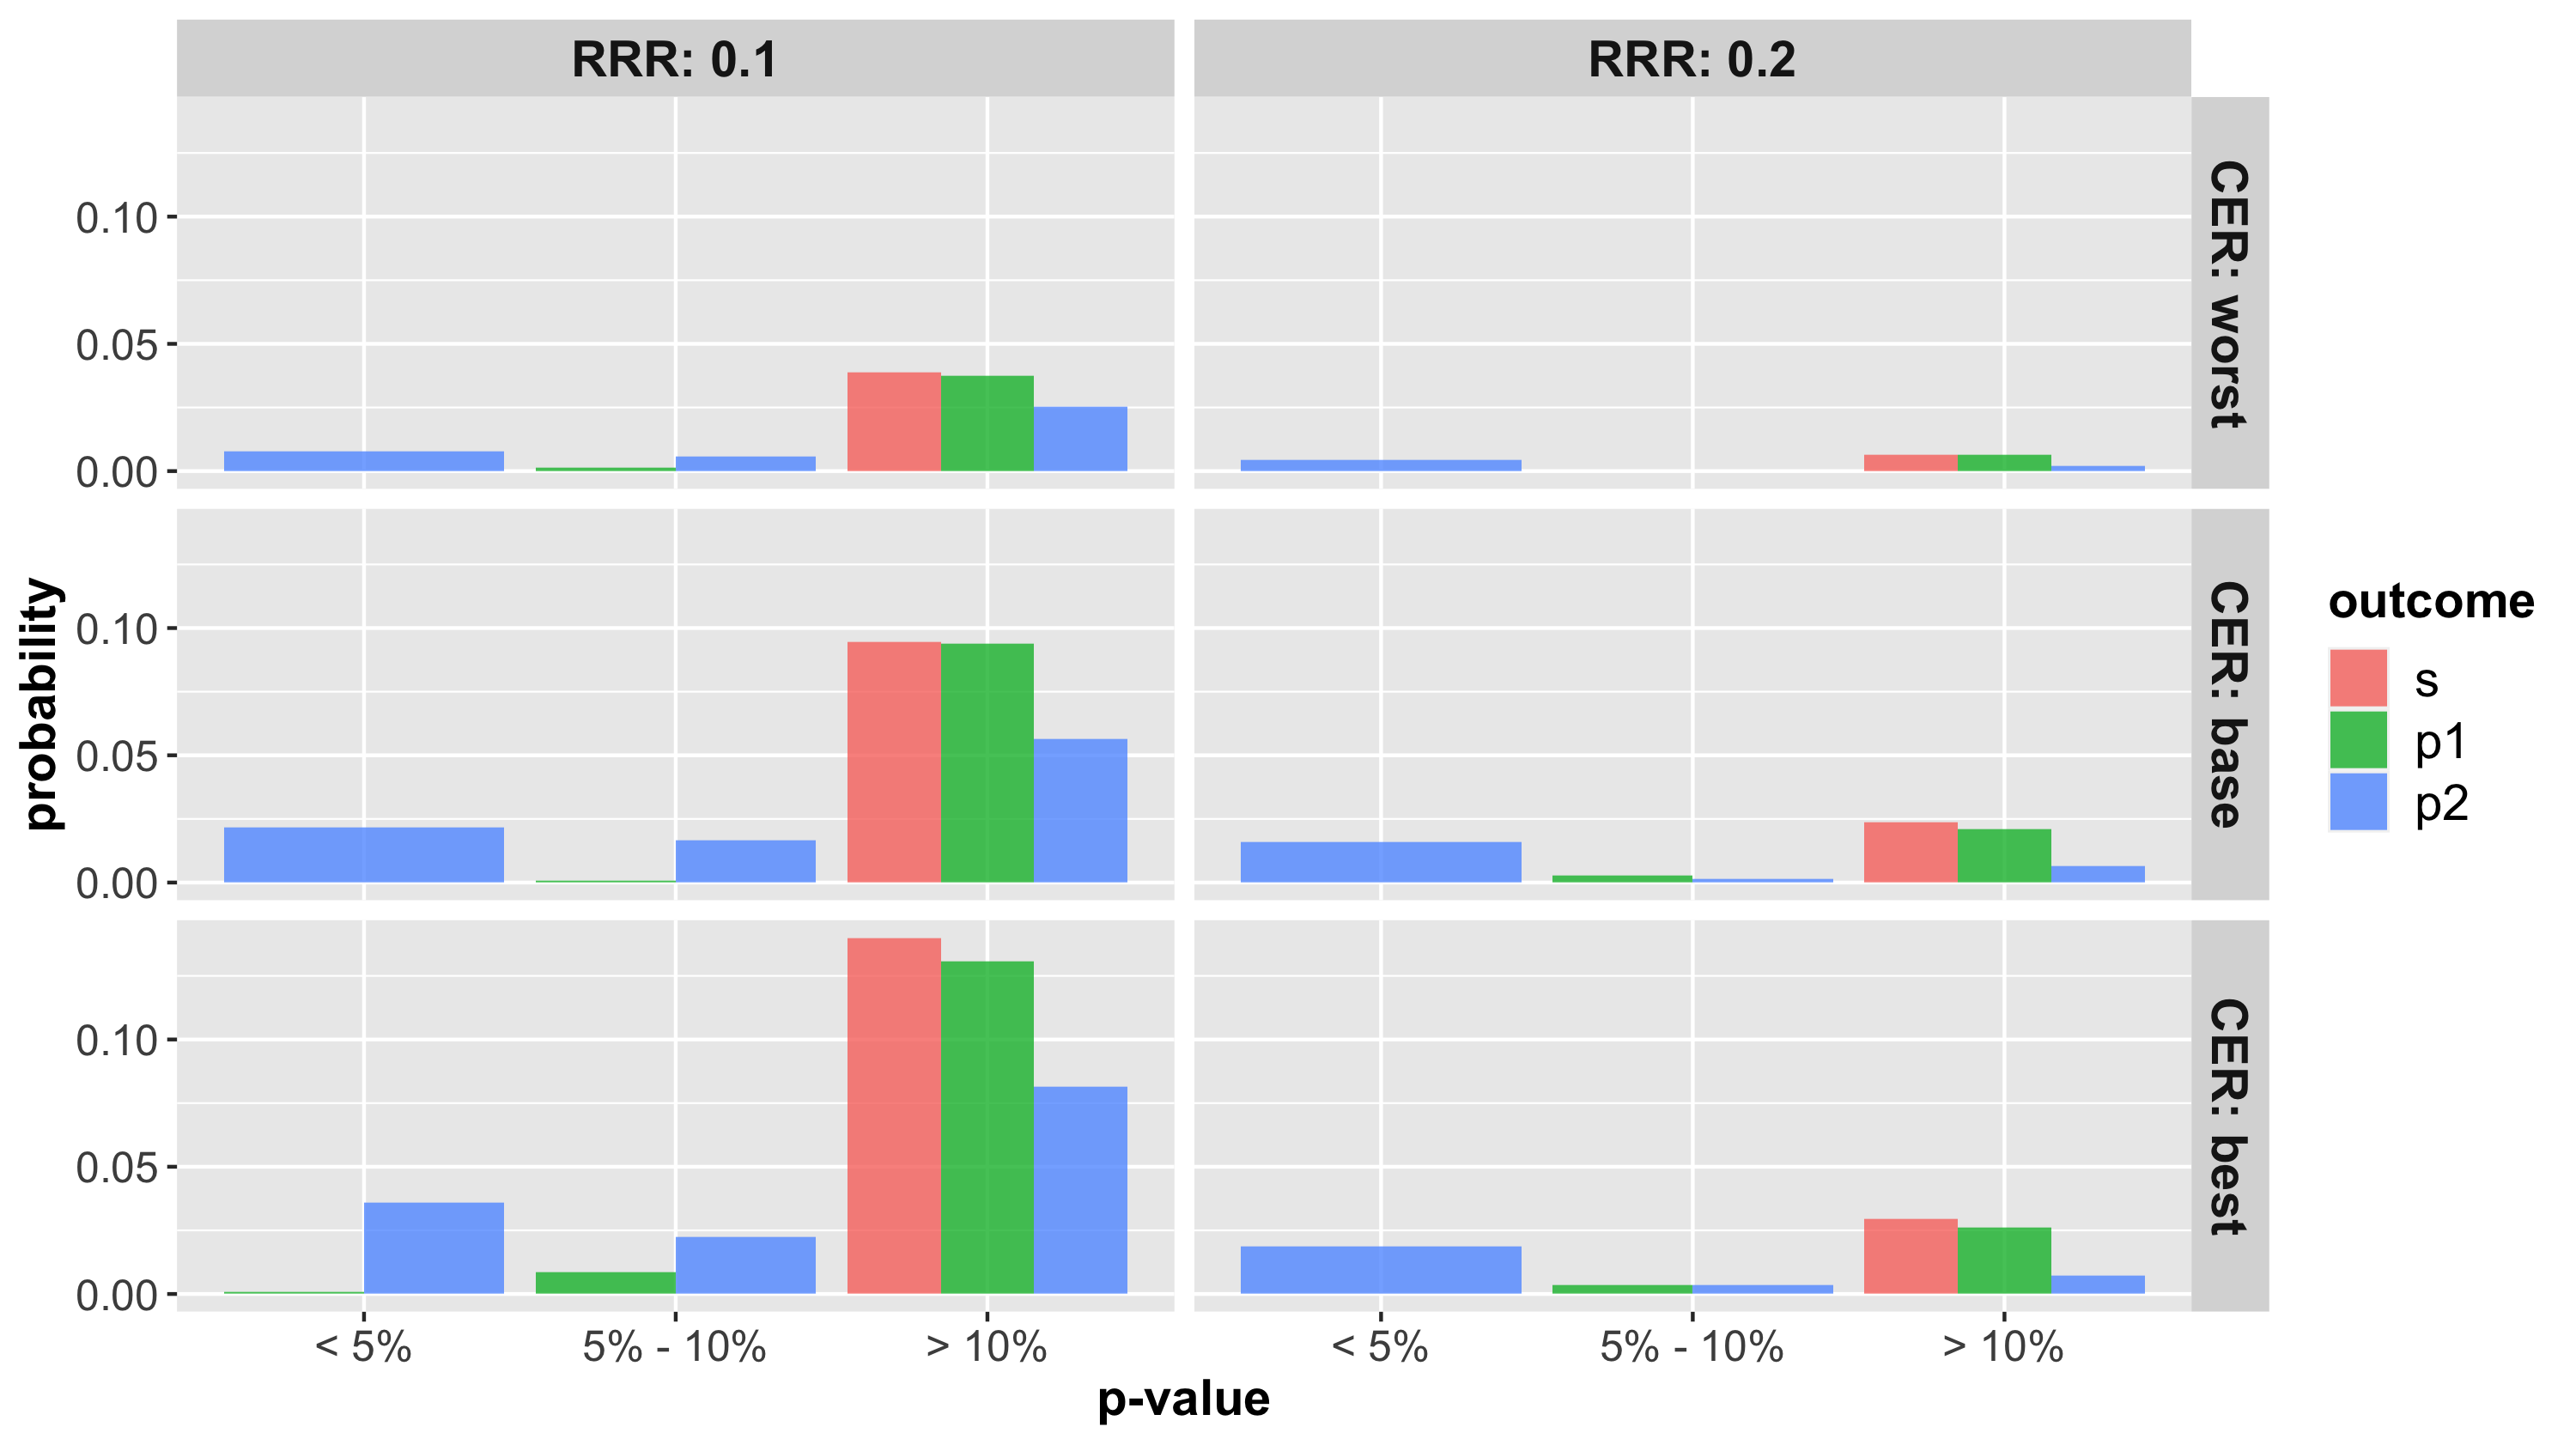
\includegraphics{../p1_plots/batch_size_nb_2000/pvalue_fut_p1.png}
  \end{subfigure}
  \bigbreak
  \begin{subfigure}{0.8\textwidth}
    \centering
    \caption{}
    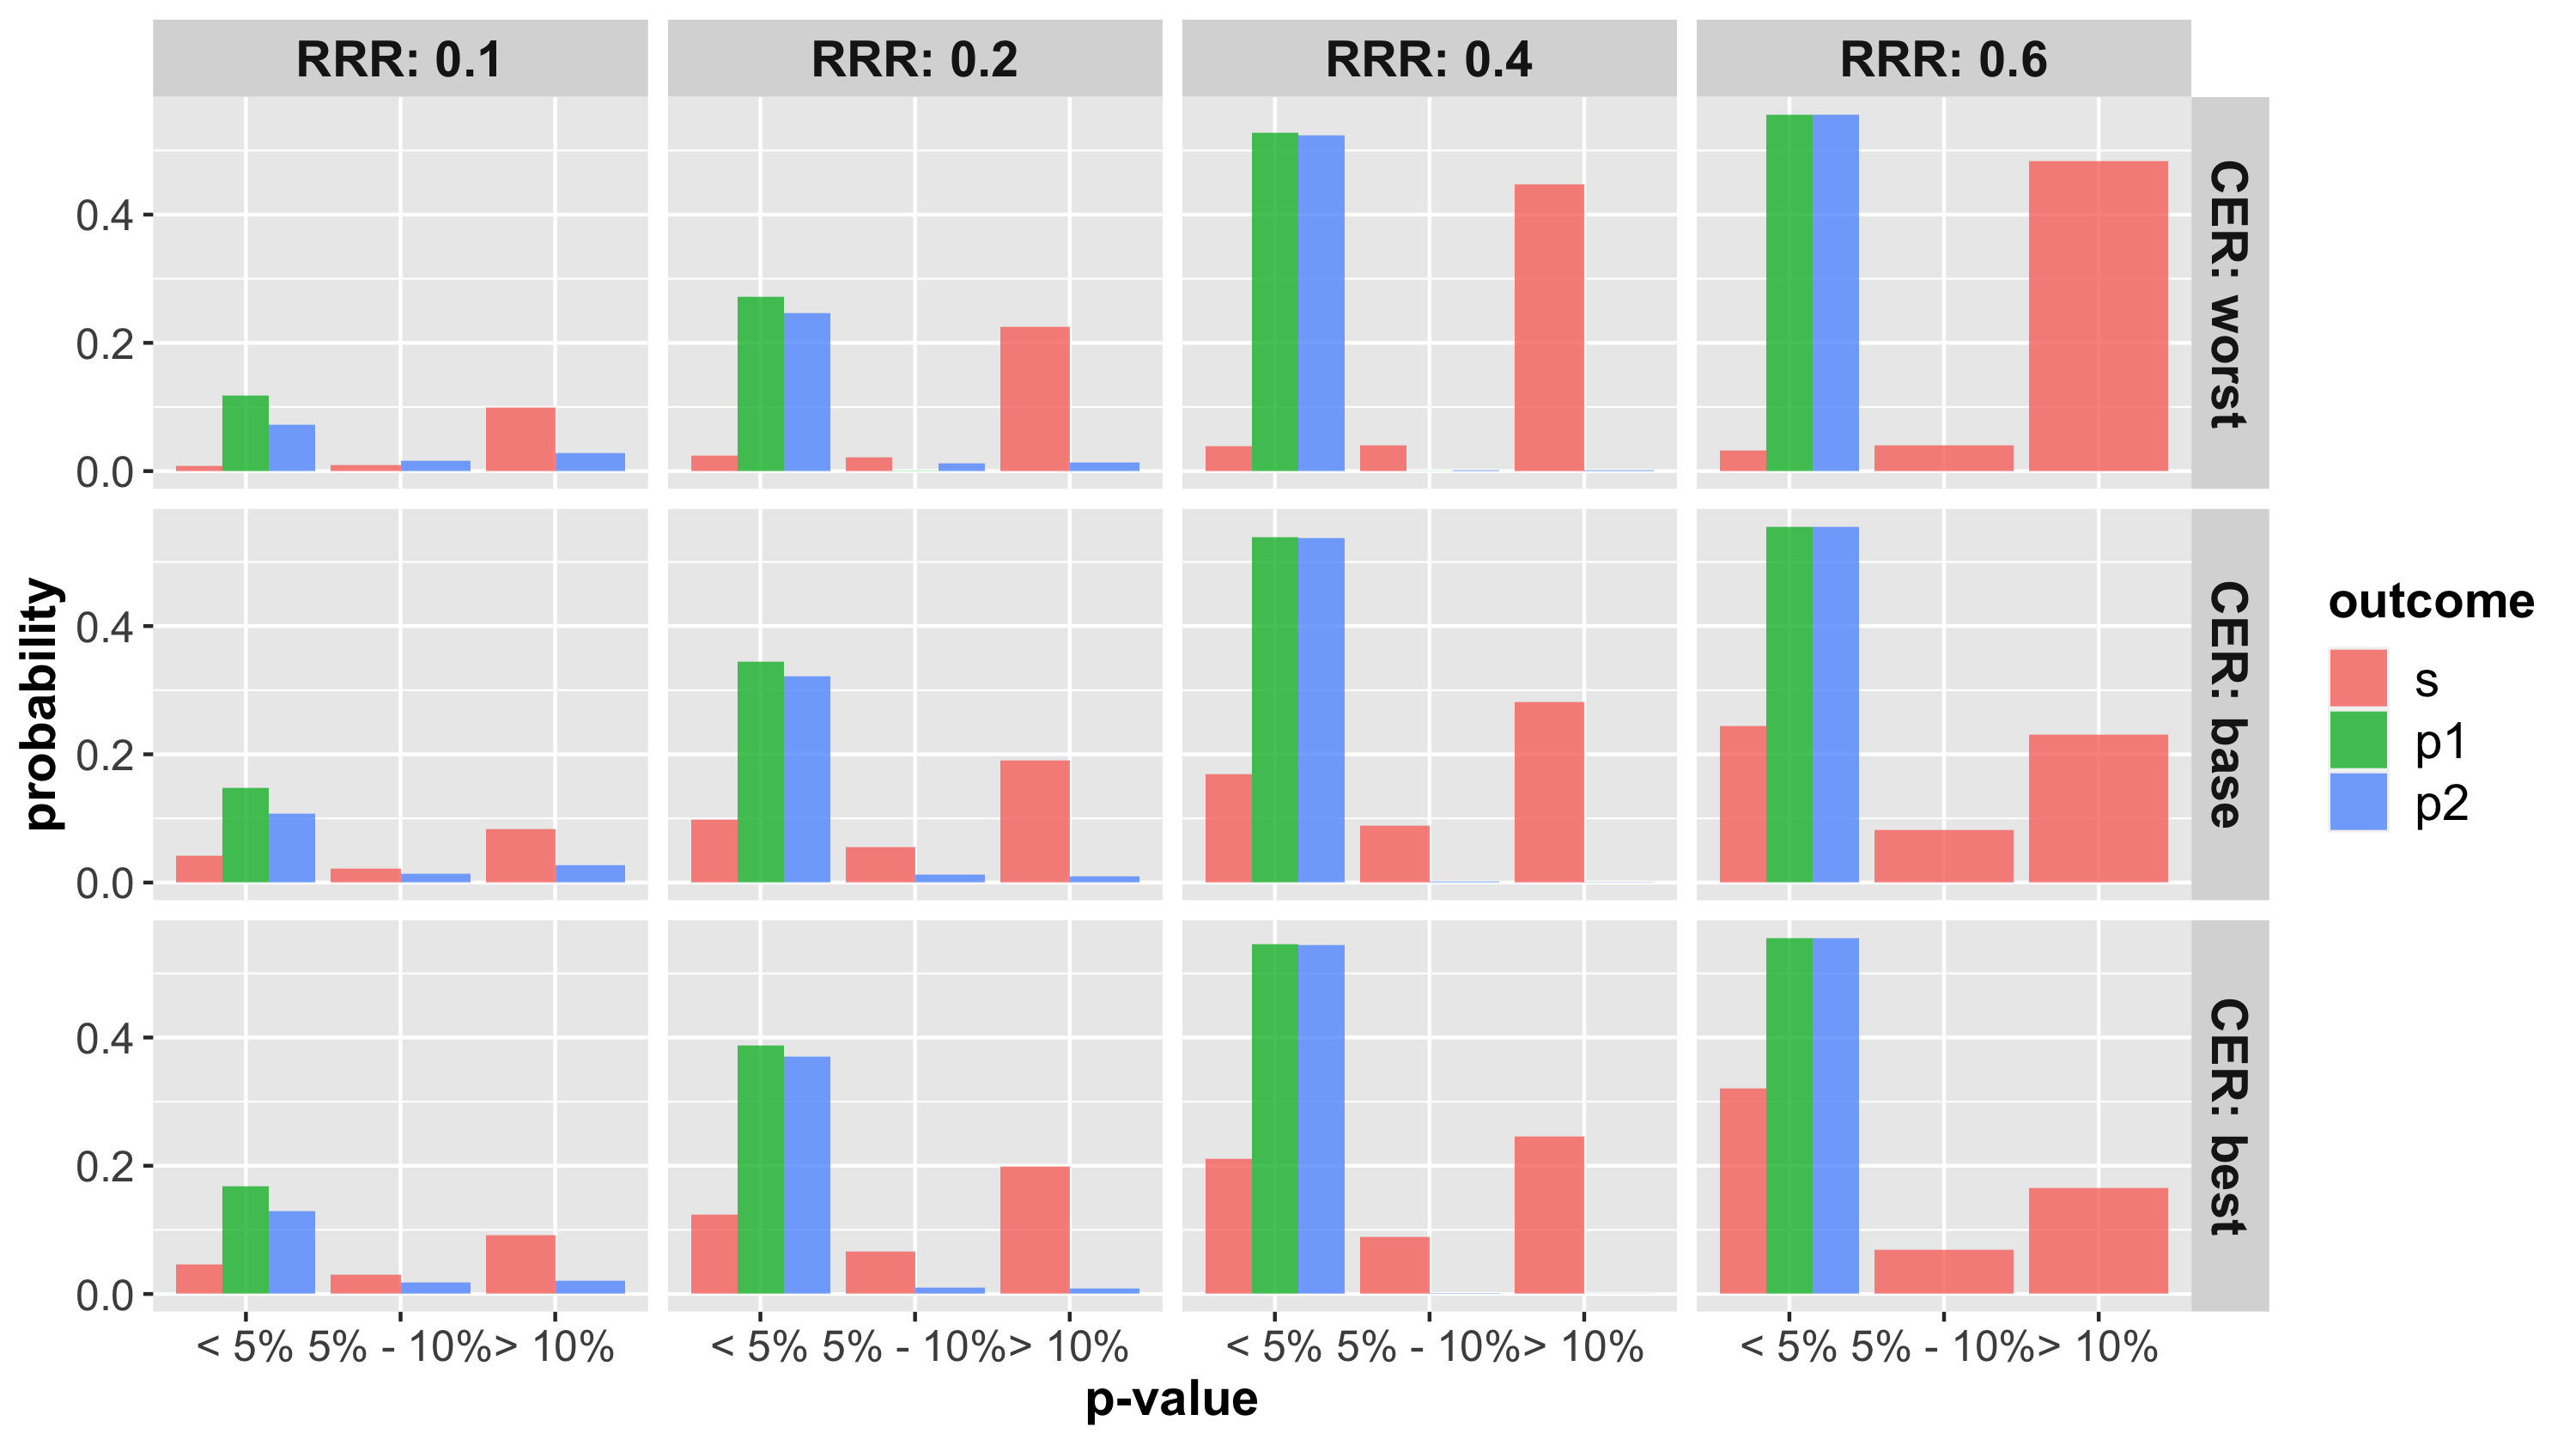
\includegraphics{../p1_plots/batch_size_nb_2000/pvalue_sup_p1.png}
  \end{subfigure}
\end{figure}

\hypertarget{relative-risk-reduction-estimates-at-trial-termination-1}{%
\paragraph{Relative risk reduction estimates at trial
termination}\label{relative-risk-reduction-estimates-at-trial-termination-1}}

\begin{figure}
  \caption{Distribution of relative risk reduction estimates (smoothed by a kernel density estimator) for the three
  control event rates (CER – rows), four relative risk reductions (RRR – columns) and the three outcomes (legend).}
  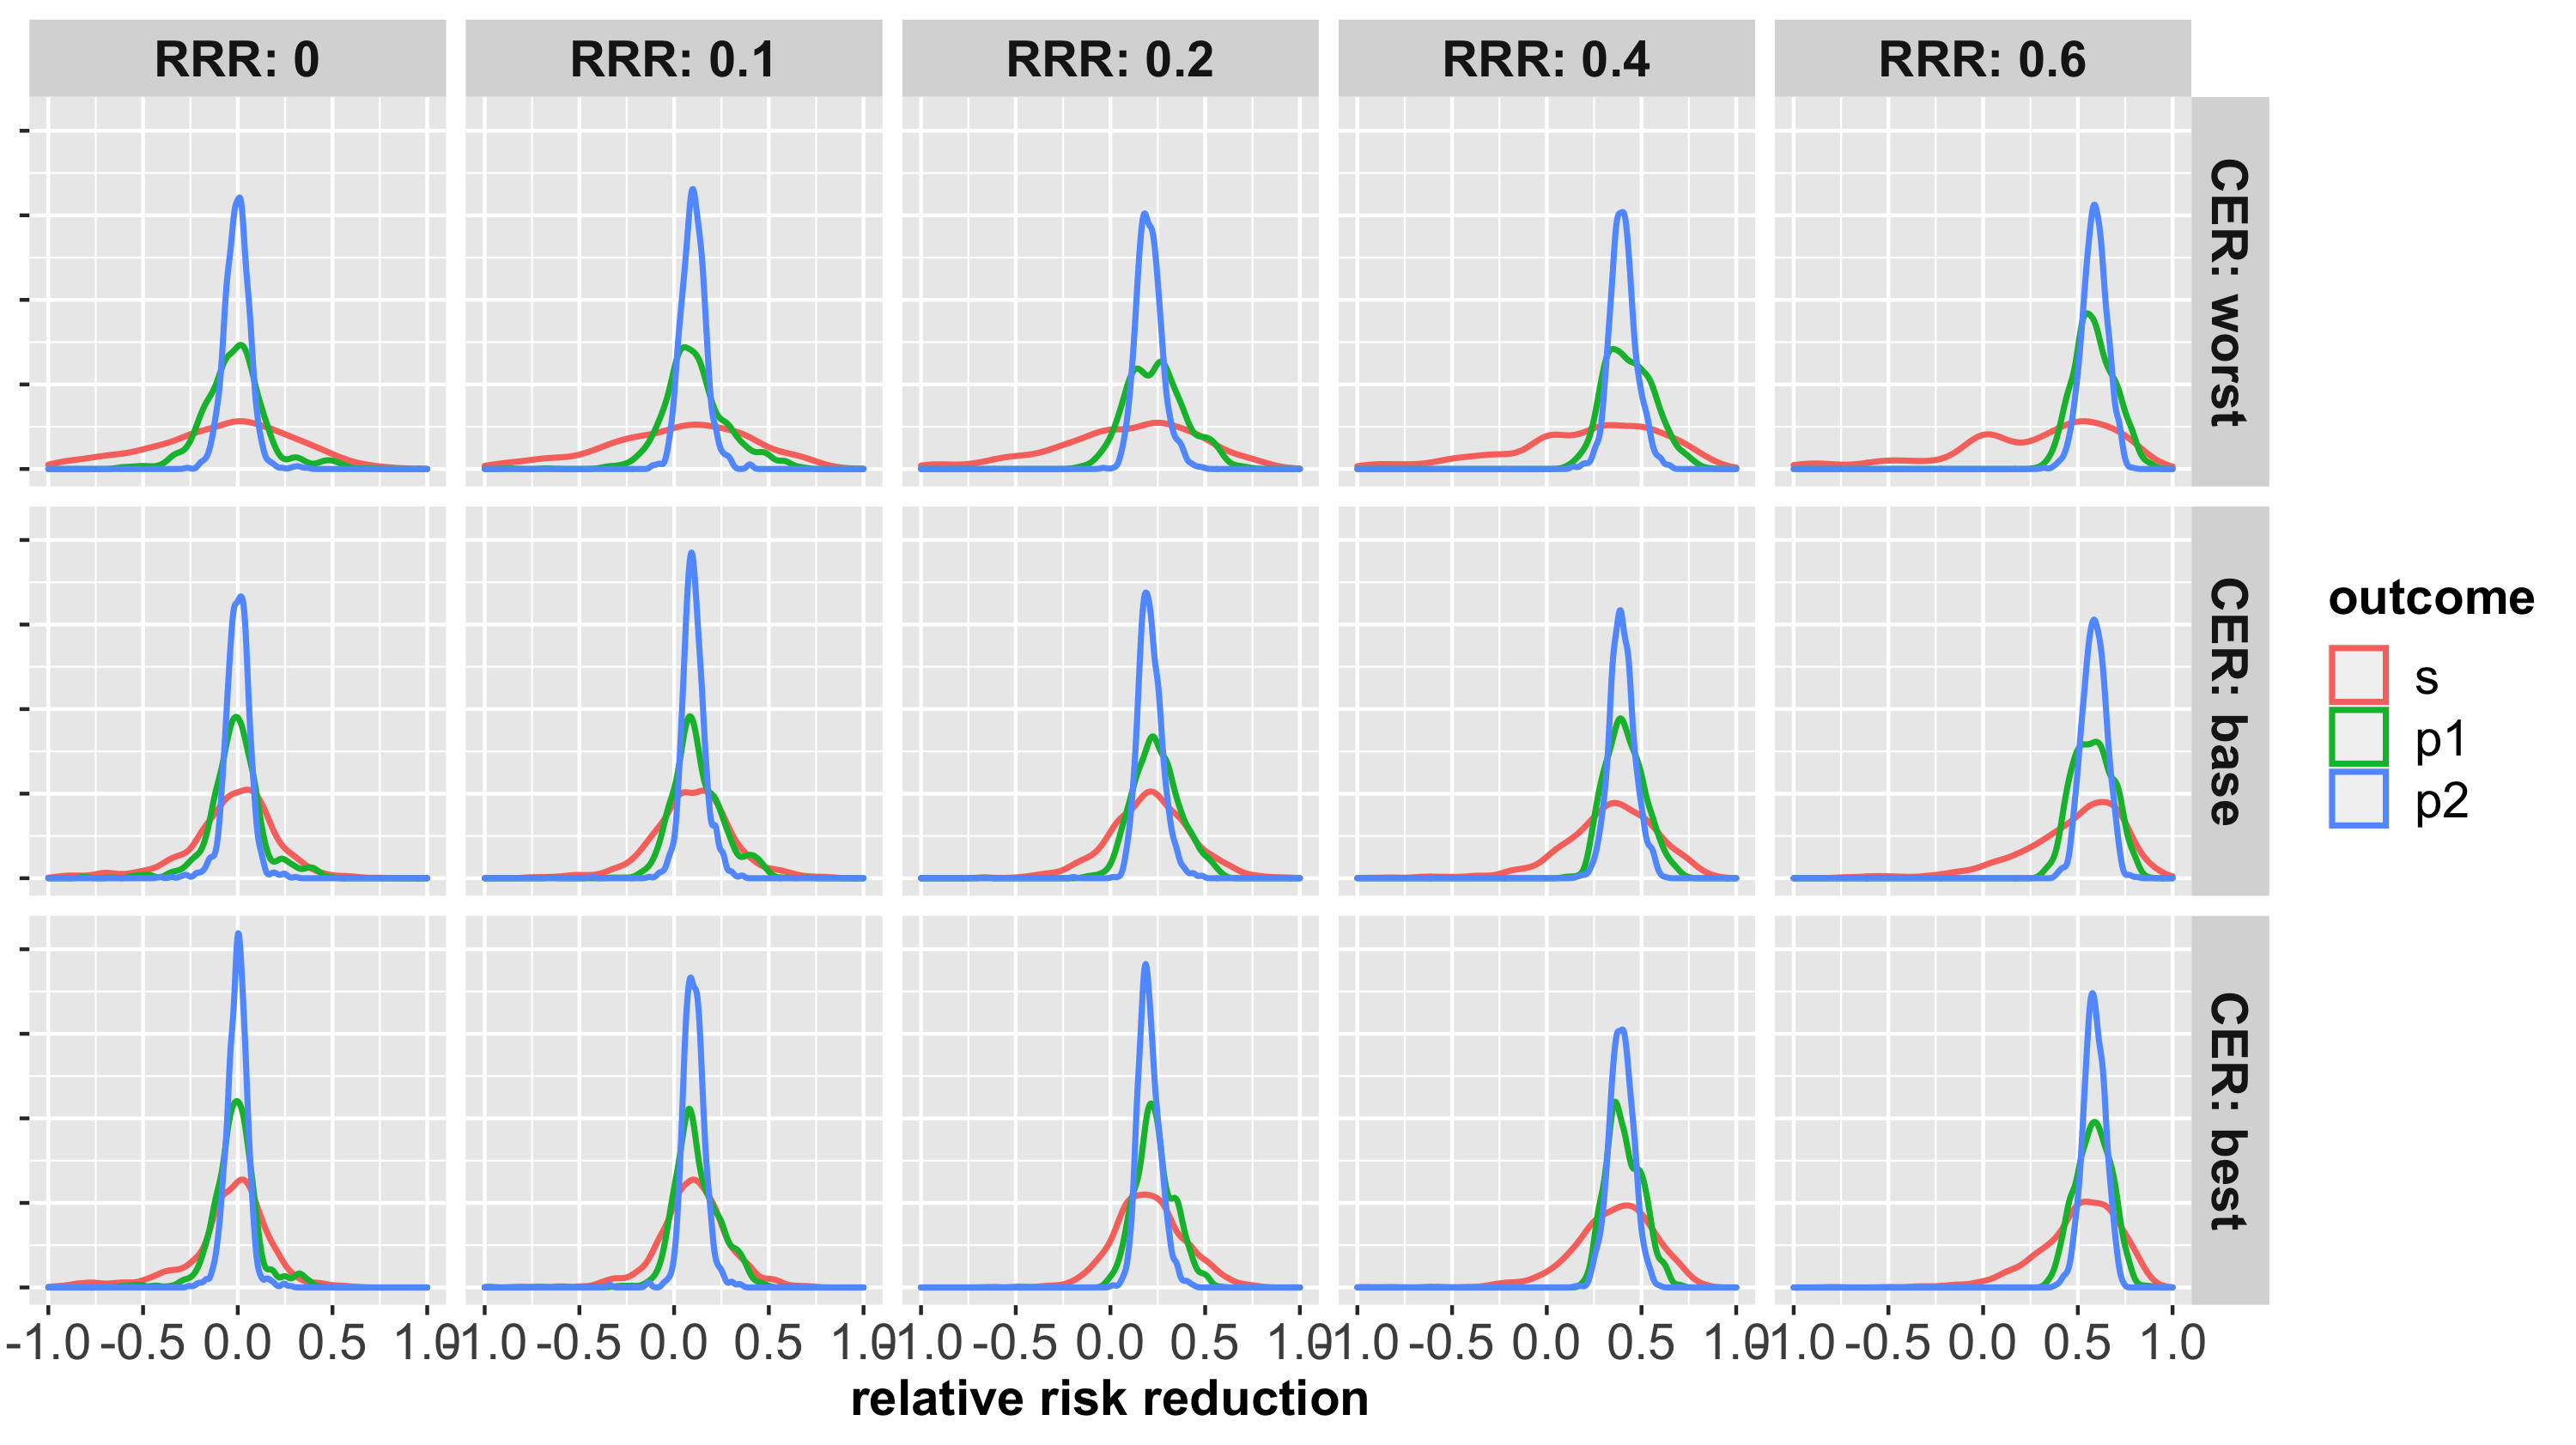
\includegraphics{../p1_plots/batch_size_nb_2000/RRRhat_p1.png}
\end{figure}

\begin{figure}
\centering
  \caption{Distribution of relative risk reduction estimates after stopping early for (a) futility; (b) superiority.
  Results are presented for the three control event rates by rows, four relative risk reductions (by columns) and the
  three outcomes (legend).}
  \begin{subfigure}{0.8\textwidth}
    \centering
    \caption{}
    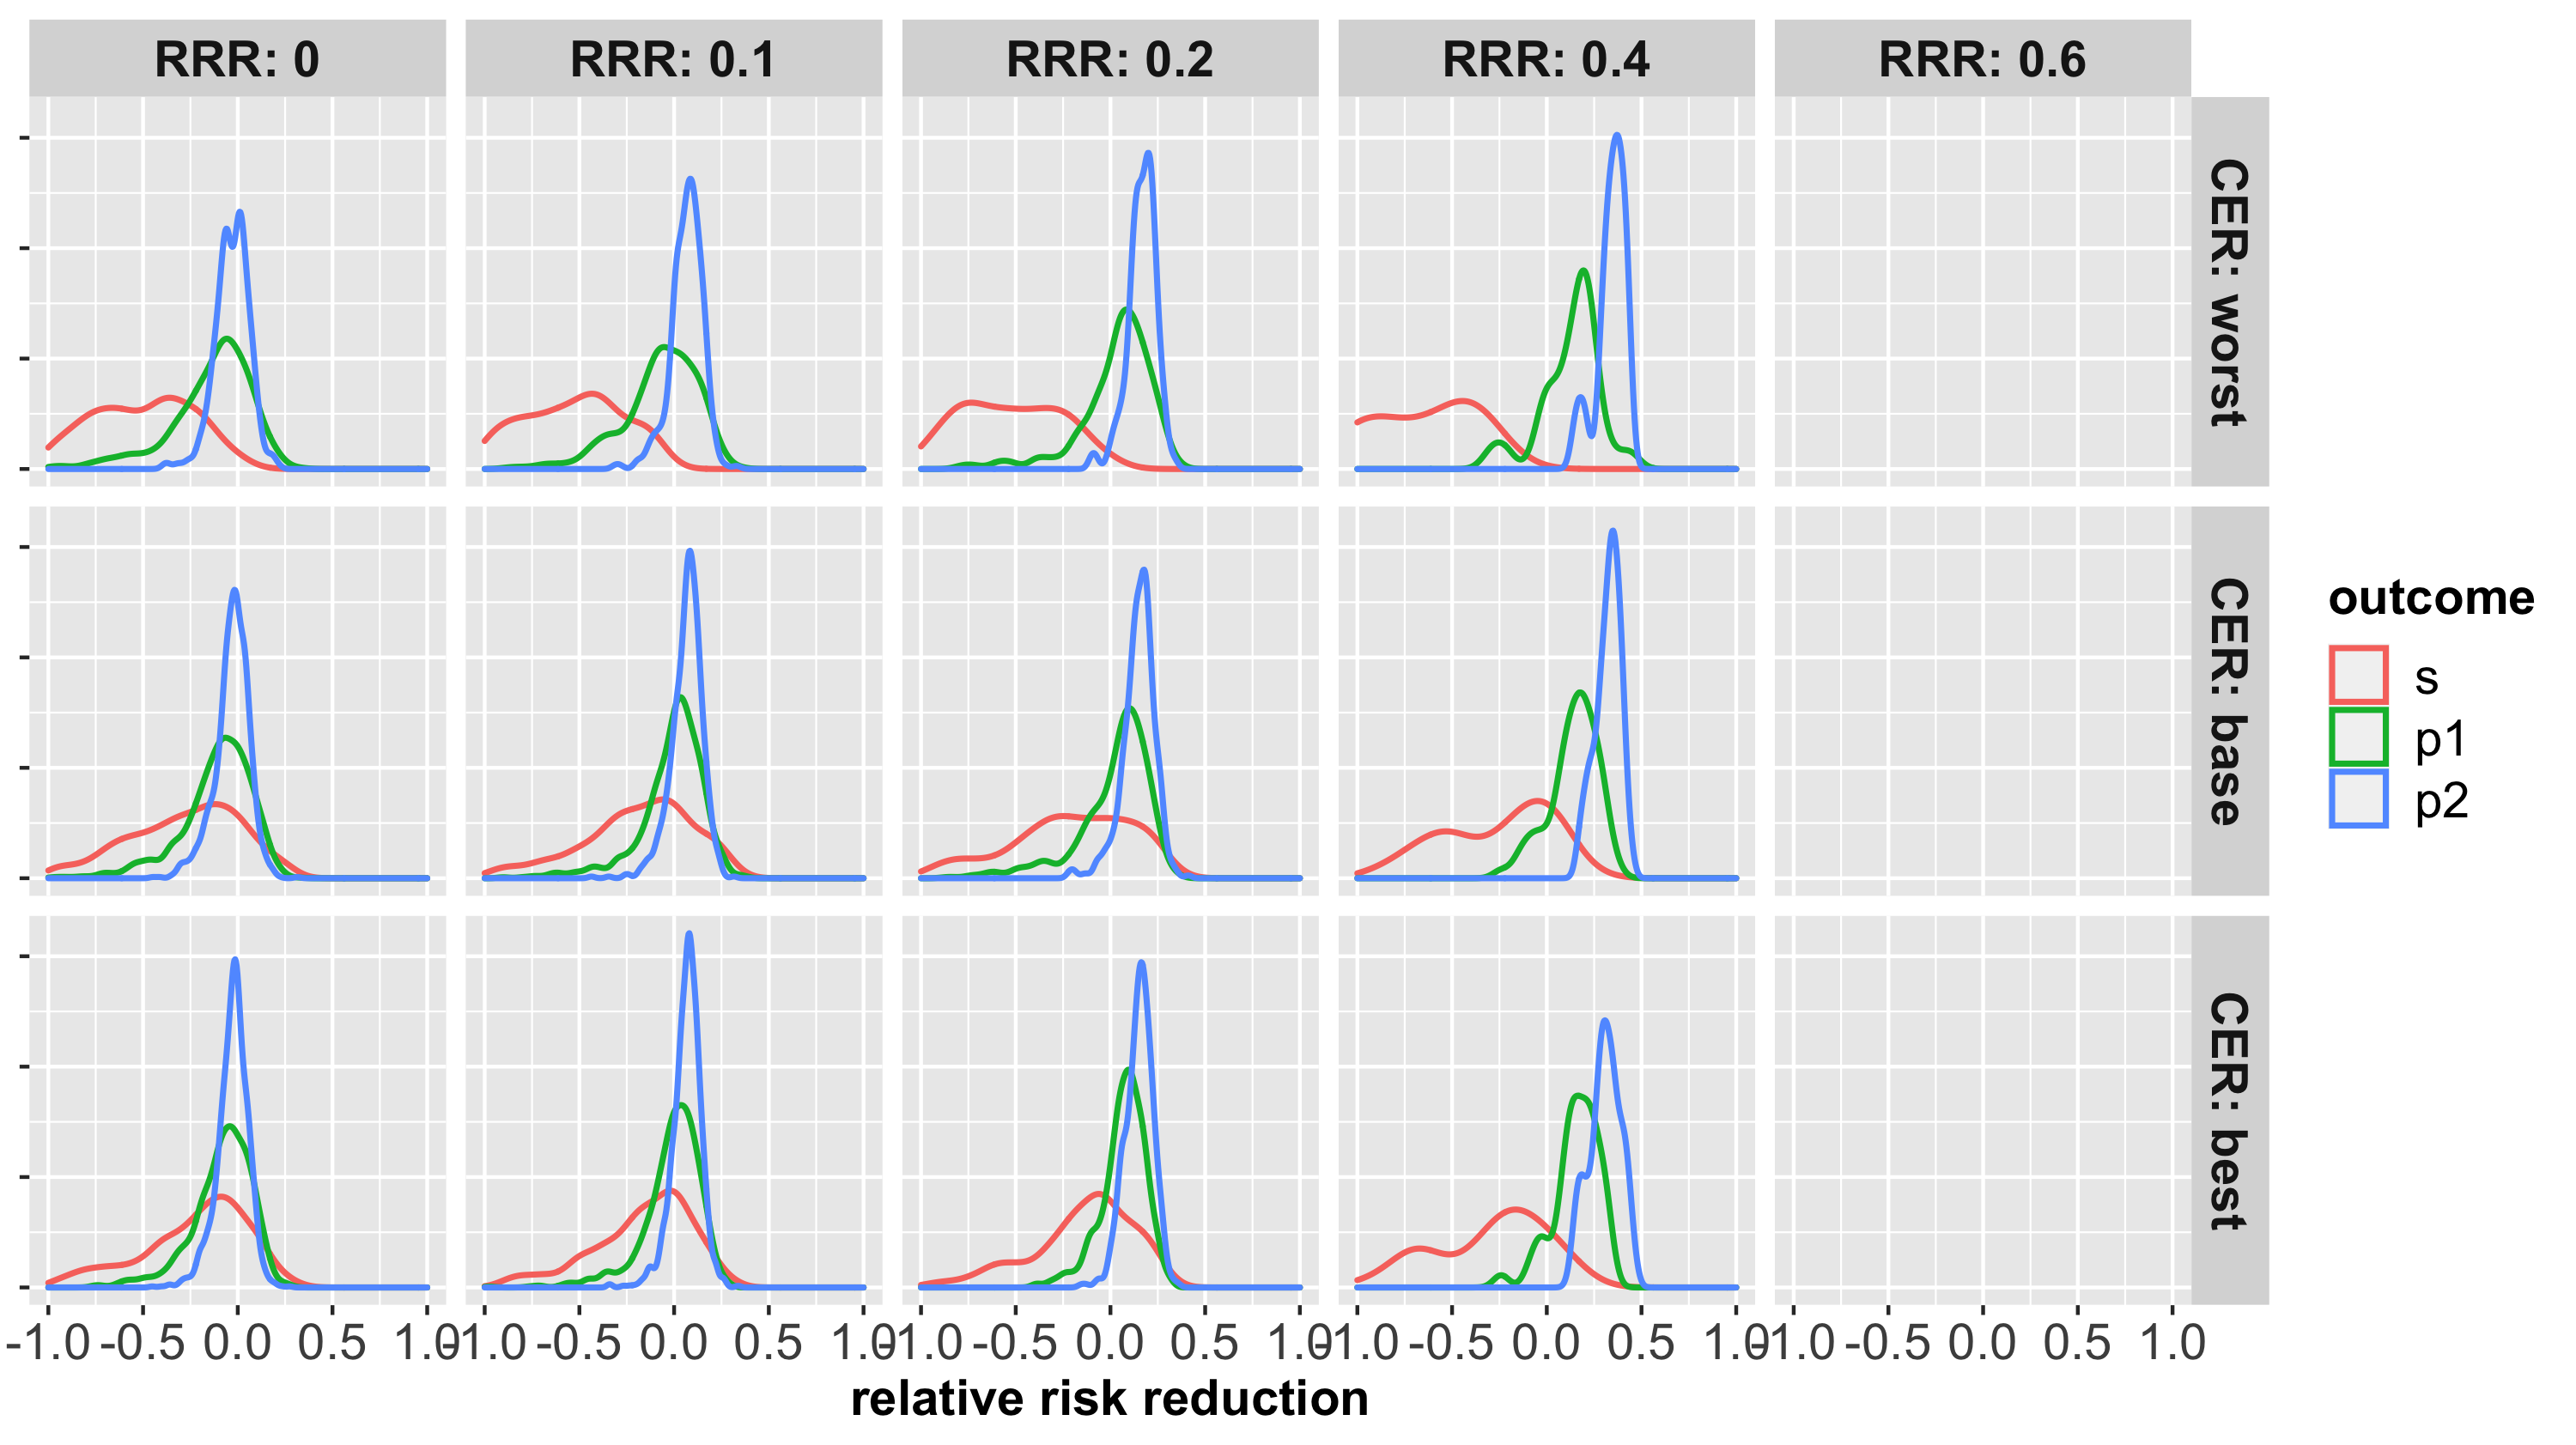
\includegraphics{../p1_plots/batch_size_nb_2000/RRRhat_fut_p1.png}
  \end{subfigure}
  \bigbreak
  \begin{subfigure}{0.8\textwidth}
    \centering
    \caption{}
    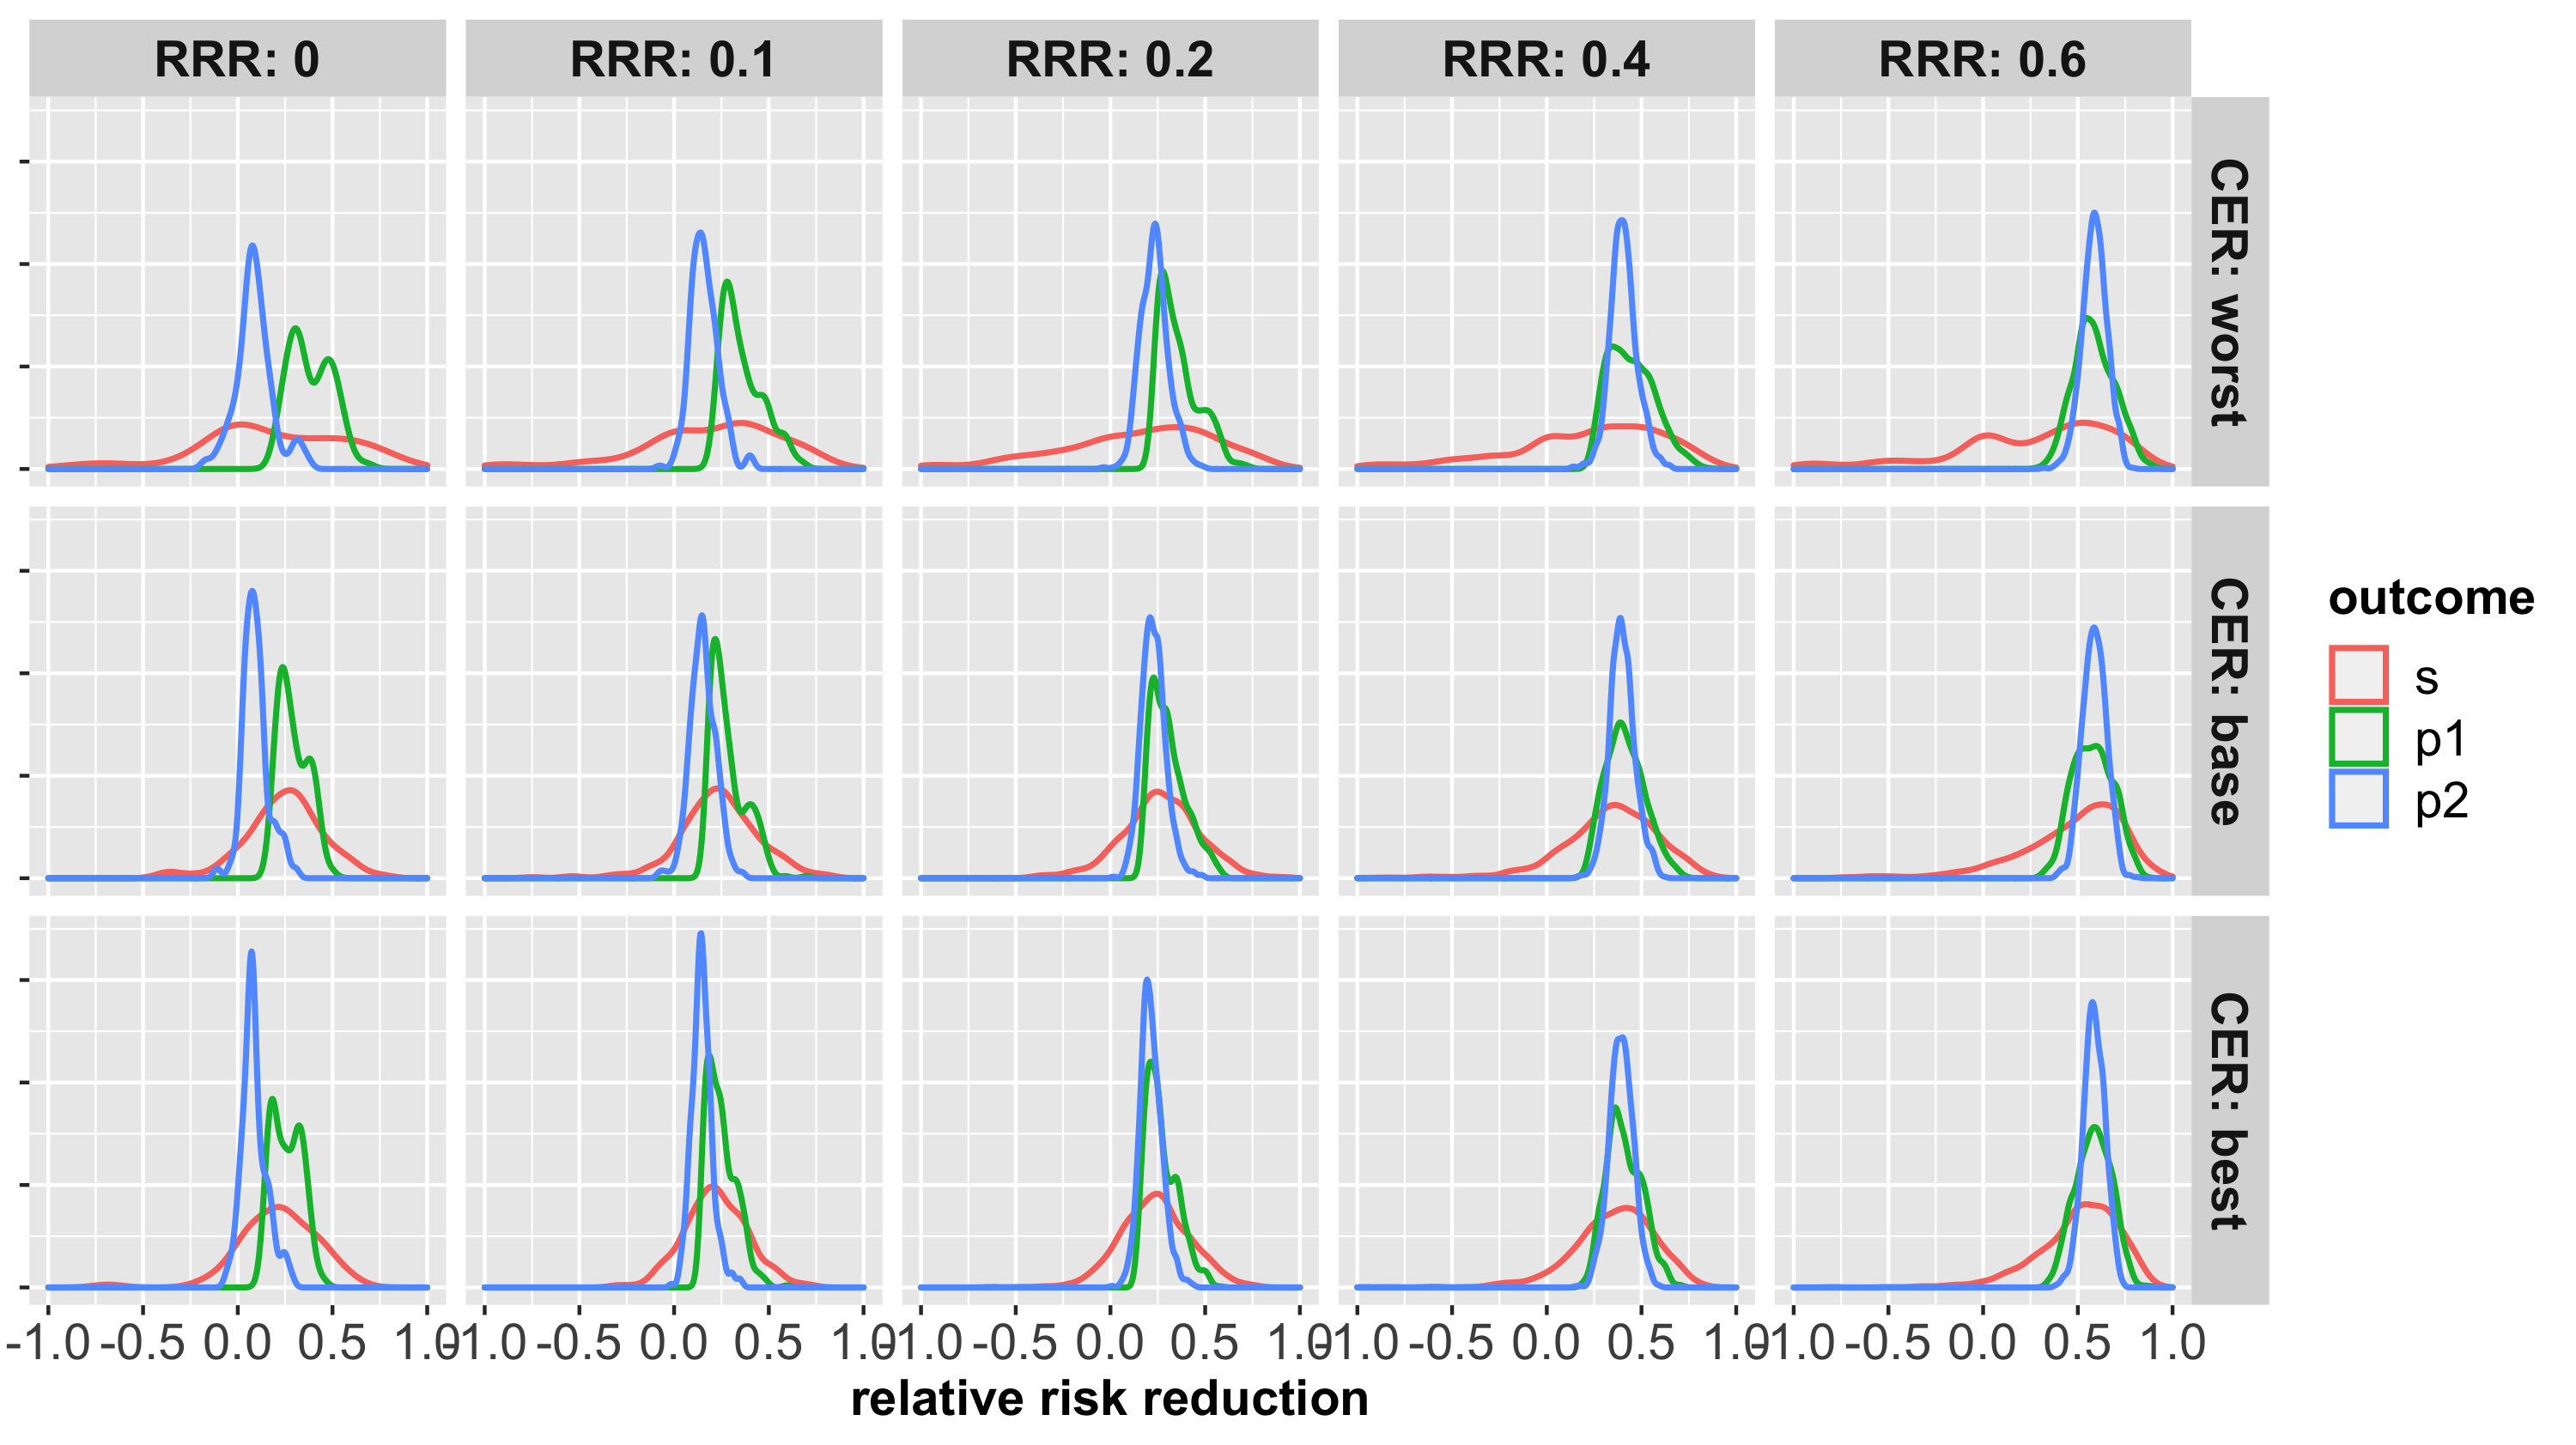
\includegraphics{../p1_plots/batch_size_nb_2000/RRRhat_sup_p1.png}
  \end{subfigure}
\end{figure}

\hypertarget{stopping-with-moderately-permissive-outcome-p1-2}{%
\subsection{Stopping with moderately permissive outcome
(p1)}\label{stopping-with-moderately-permissive-outcome-p1-2}}

\hypertarget{maximum-allowed-sample-size-of-12000-with-interim-analyses-conducted-every-3000-patients}{%
\paragraph{Maximum allowed sample size of 12,000 with interim analyses
conducted every 3,000
patients}\label{maximum-allowed-sample-size-of-12000-with-interim-analyses-conducted-every-3000-patients}}

Both superiority and futility decisions were made with respect to the
moderately permissive outcome (p1). Unless stated otherwise, the
futility bound used was 0.4 and a probability threshold of 0.99 was
required to stop for futility. The number of expected interim analyses
can be thought of as the expected number of patients at trial
determination divided by the batch size, which here is 3,000 patients.
The plots below can be interpretated in the same manner as those above.

\hypertarget{type-i-error-false-positive-risk-2}{%
\subparagraph{Type I error (false positive
risk)}\label{type-i-error-false-positive-risk-2}}

\captionsetup[figure]{font=small,labelfont=small}

\begin{figure}
  \caption{Overall type I error rate based on moderately permissive (p1) outcome based stopping rules.Observed type one error rate for each outcome is
  presented by colored bars (see legend). Results by the three categories of control event rates are by rows. Results by the futility thresholds are
  presented on the x-axis.}
  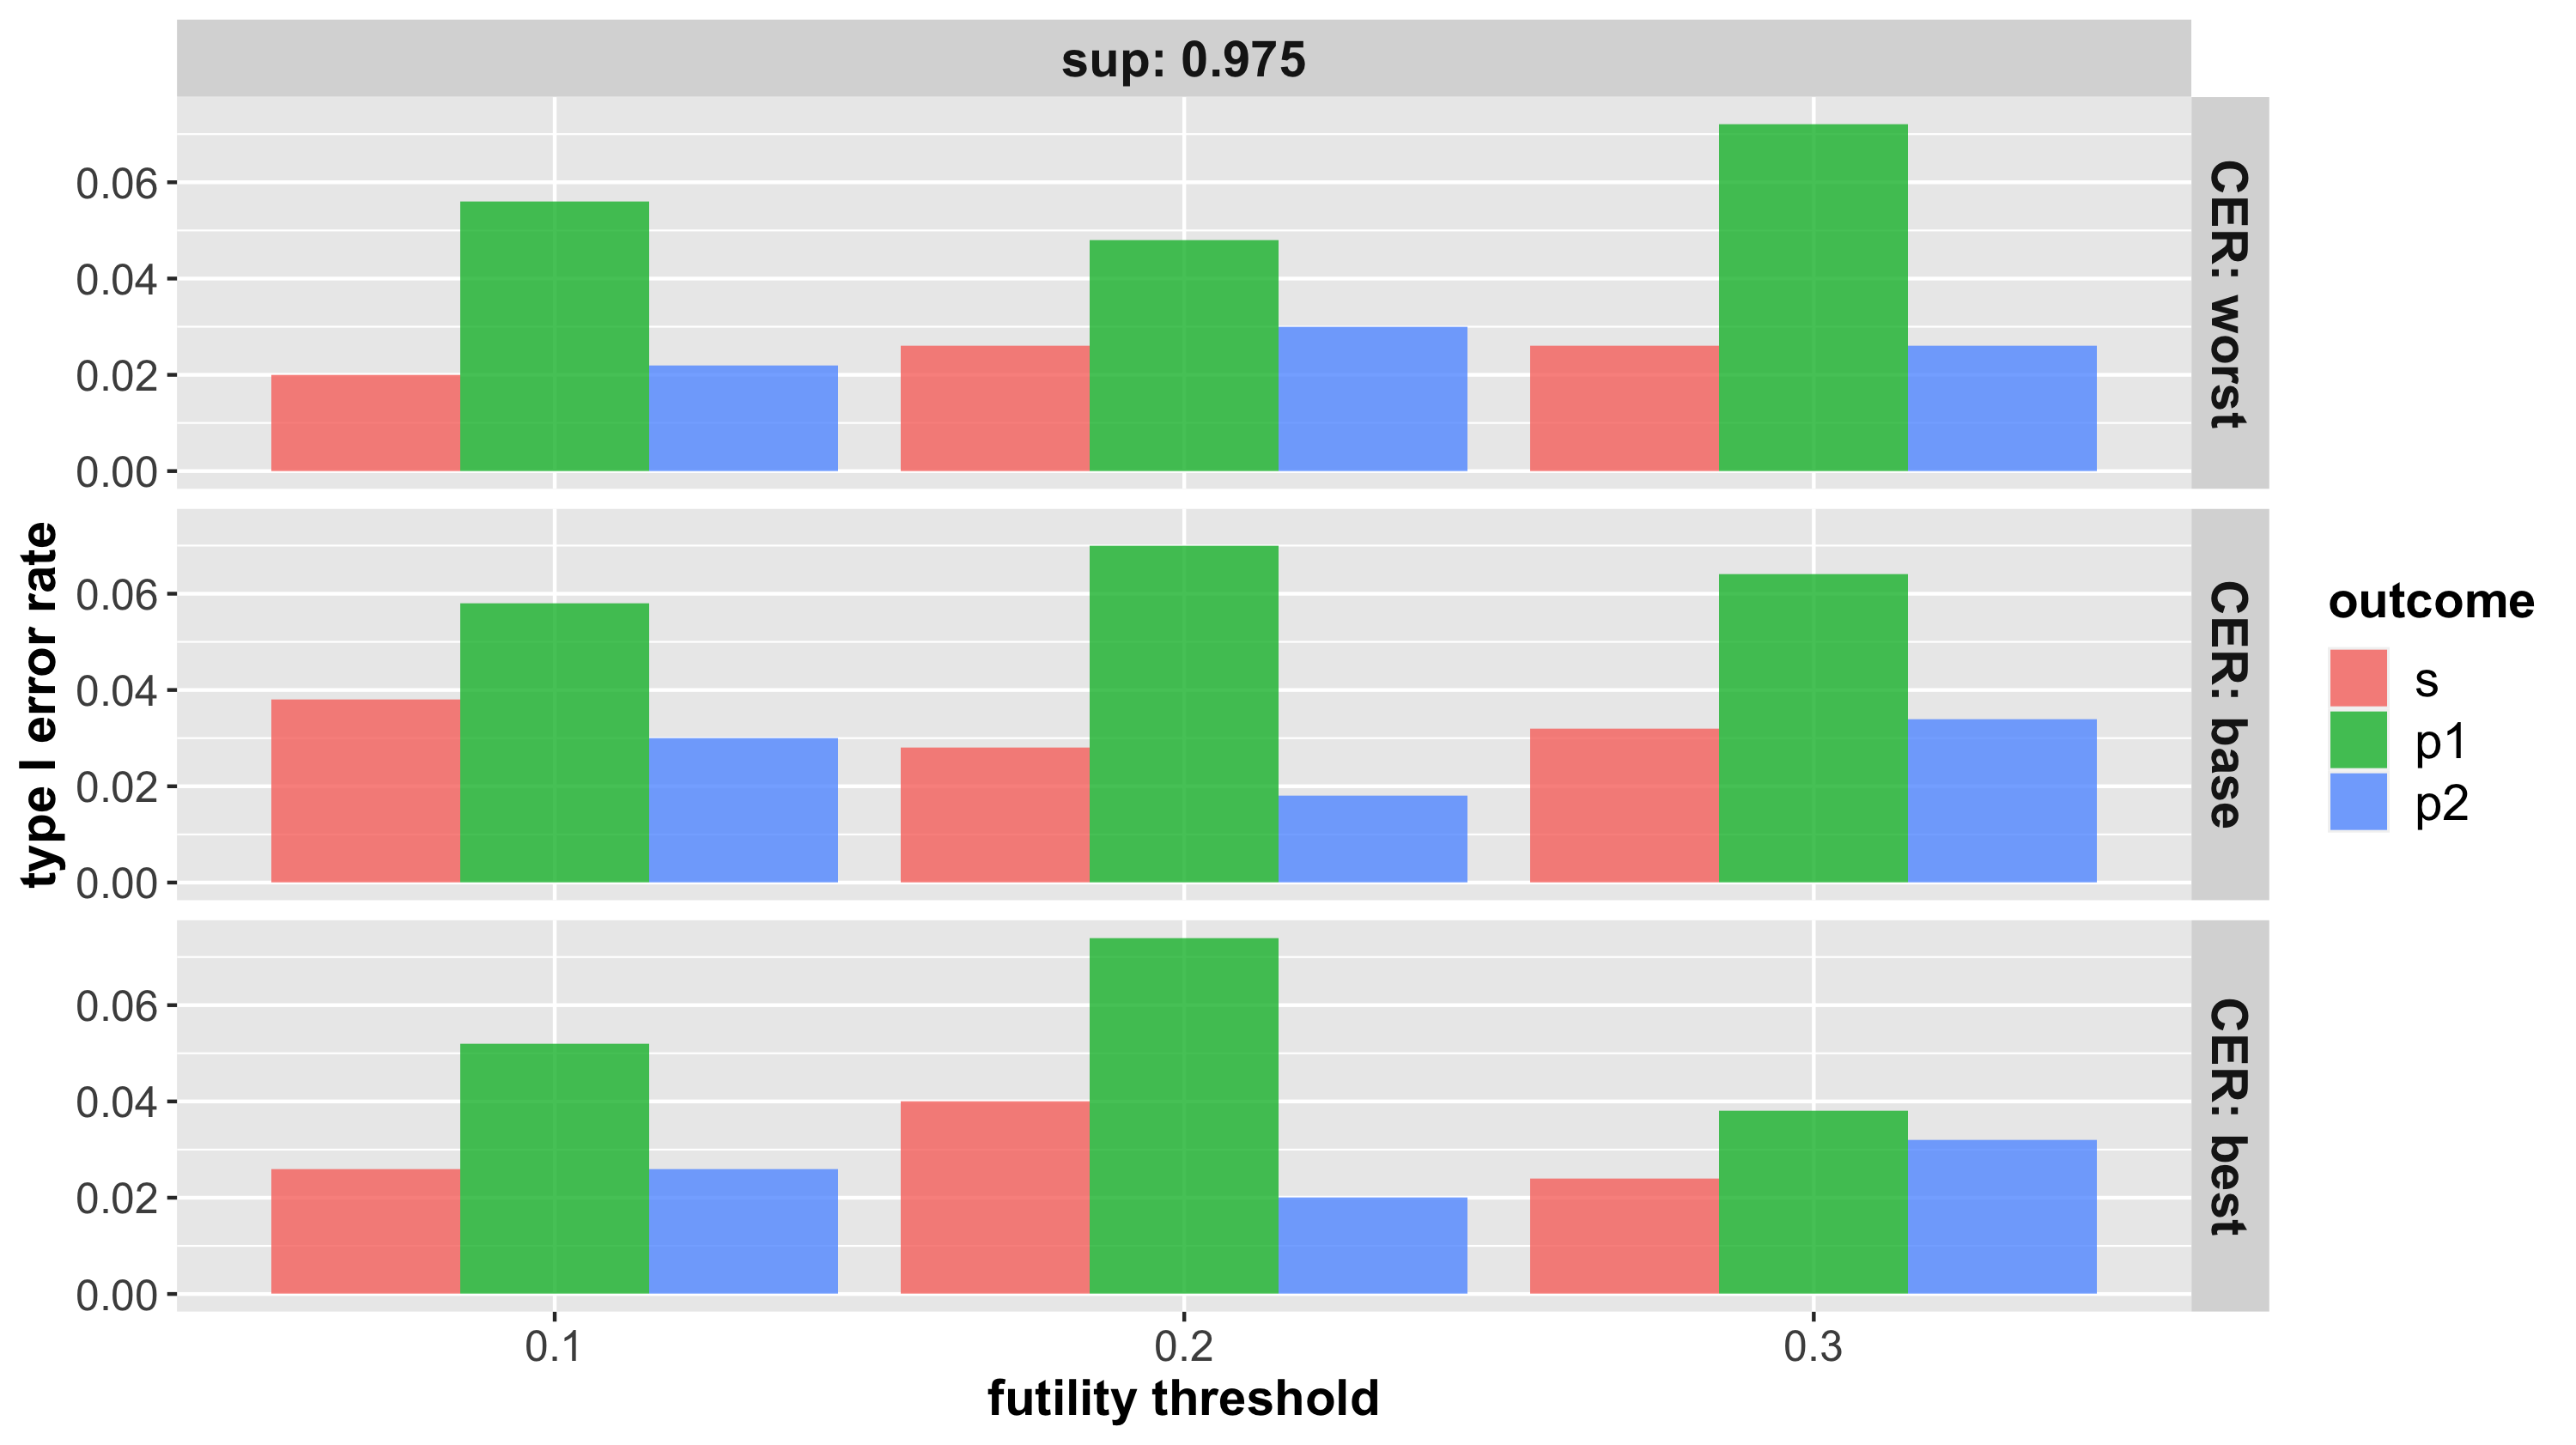
\includegraphics{../p1_plots/batch_size_nb_3000/type_1_error_p1.png}
\end{figure}

\hypertarget{power-2}{%
\subparagraph{Power}\label{power-2}}

\begin{figure}
  \caption{Power under the three relative risk reductions (RRR - upper column label) for each of the outcomes (lower column labels). 
  Power estimates by control event rates are presented by the rows. Power estimates by the futility thresholds are presented by the bar color (see legend).}
  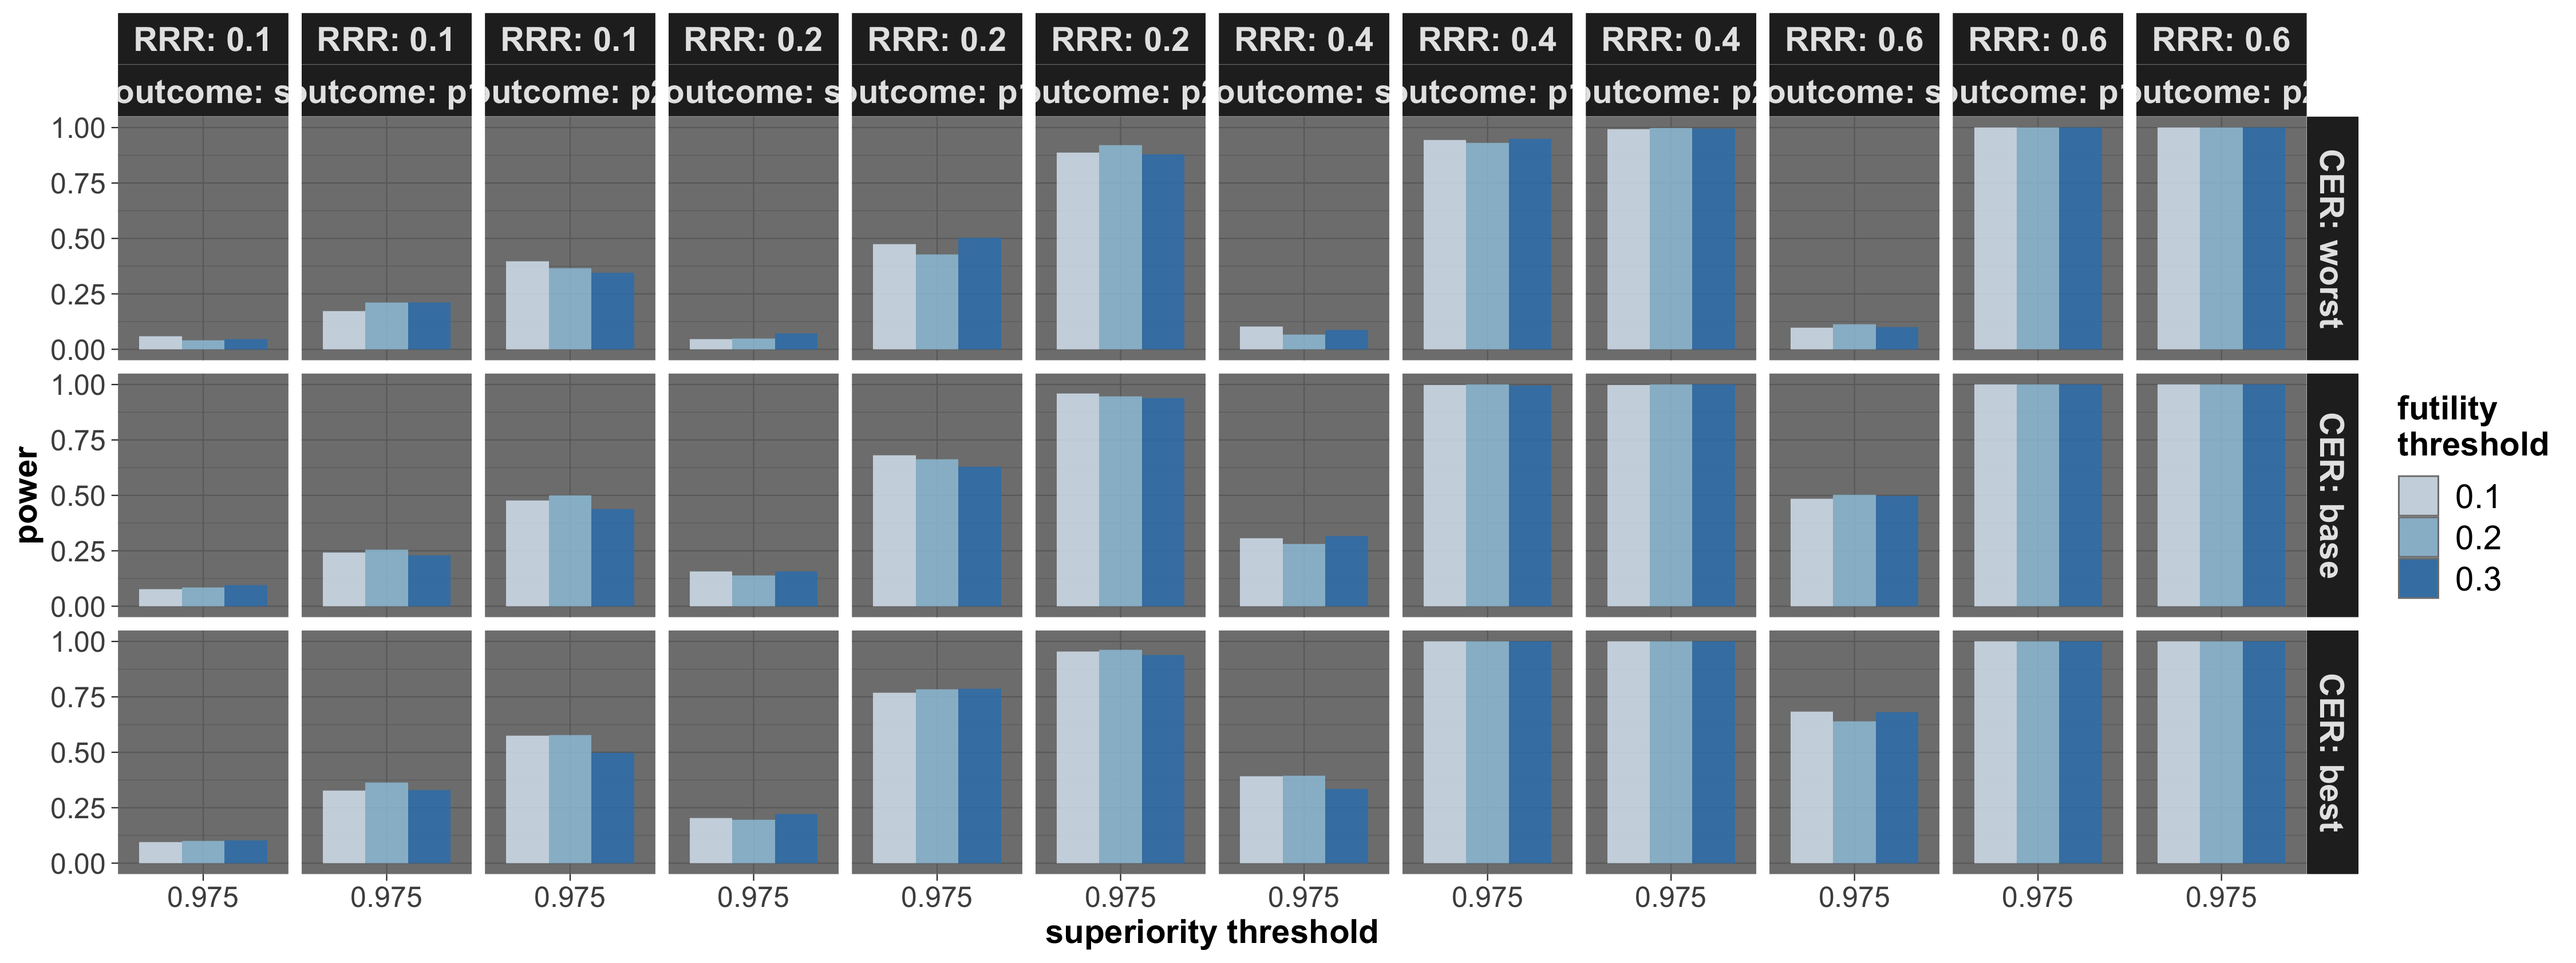
\includegraphics{../p1_plots/batch_size_nb_3000/power_all_p1.png}
\end{figure}

\begin{figure}
  \caption{Power under the three relative risk reductions (RRR - upper column label) for each of the outcomes (lower
  column labels or legend). Observed power for each outcome is presented by colored bars. Power estimates by control
  event rates are presented by the rows and correspond to a superiority threshold of 0.975.}
  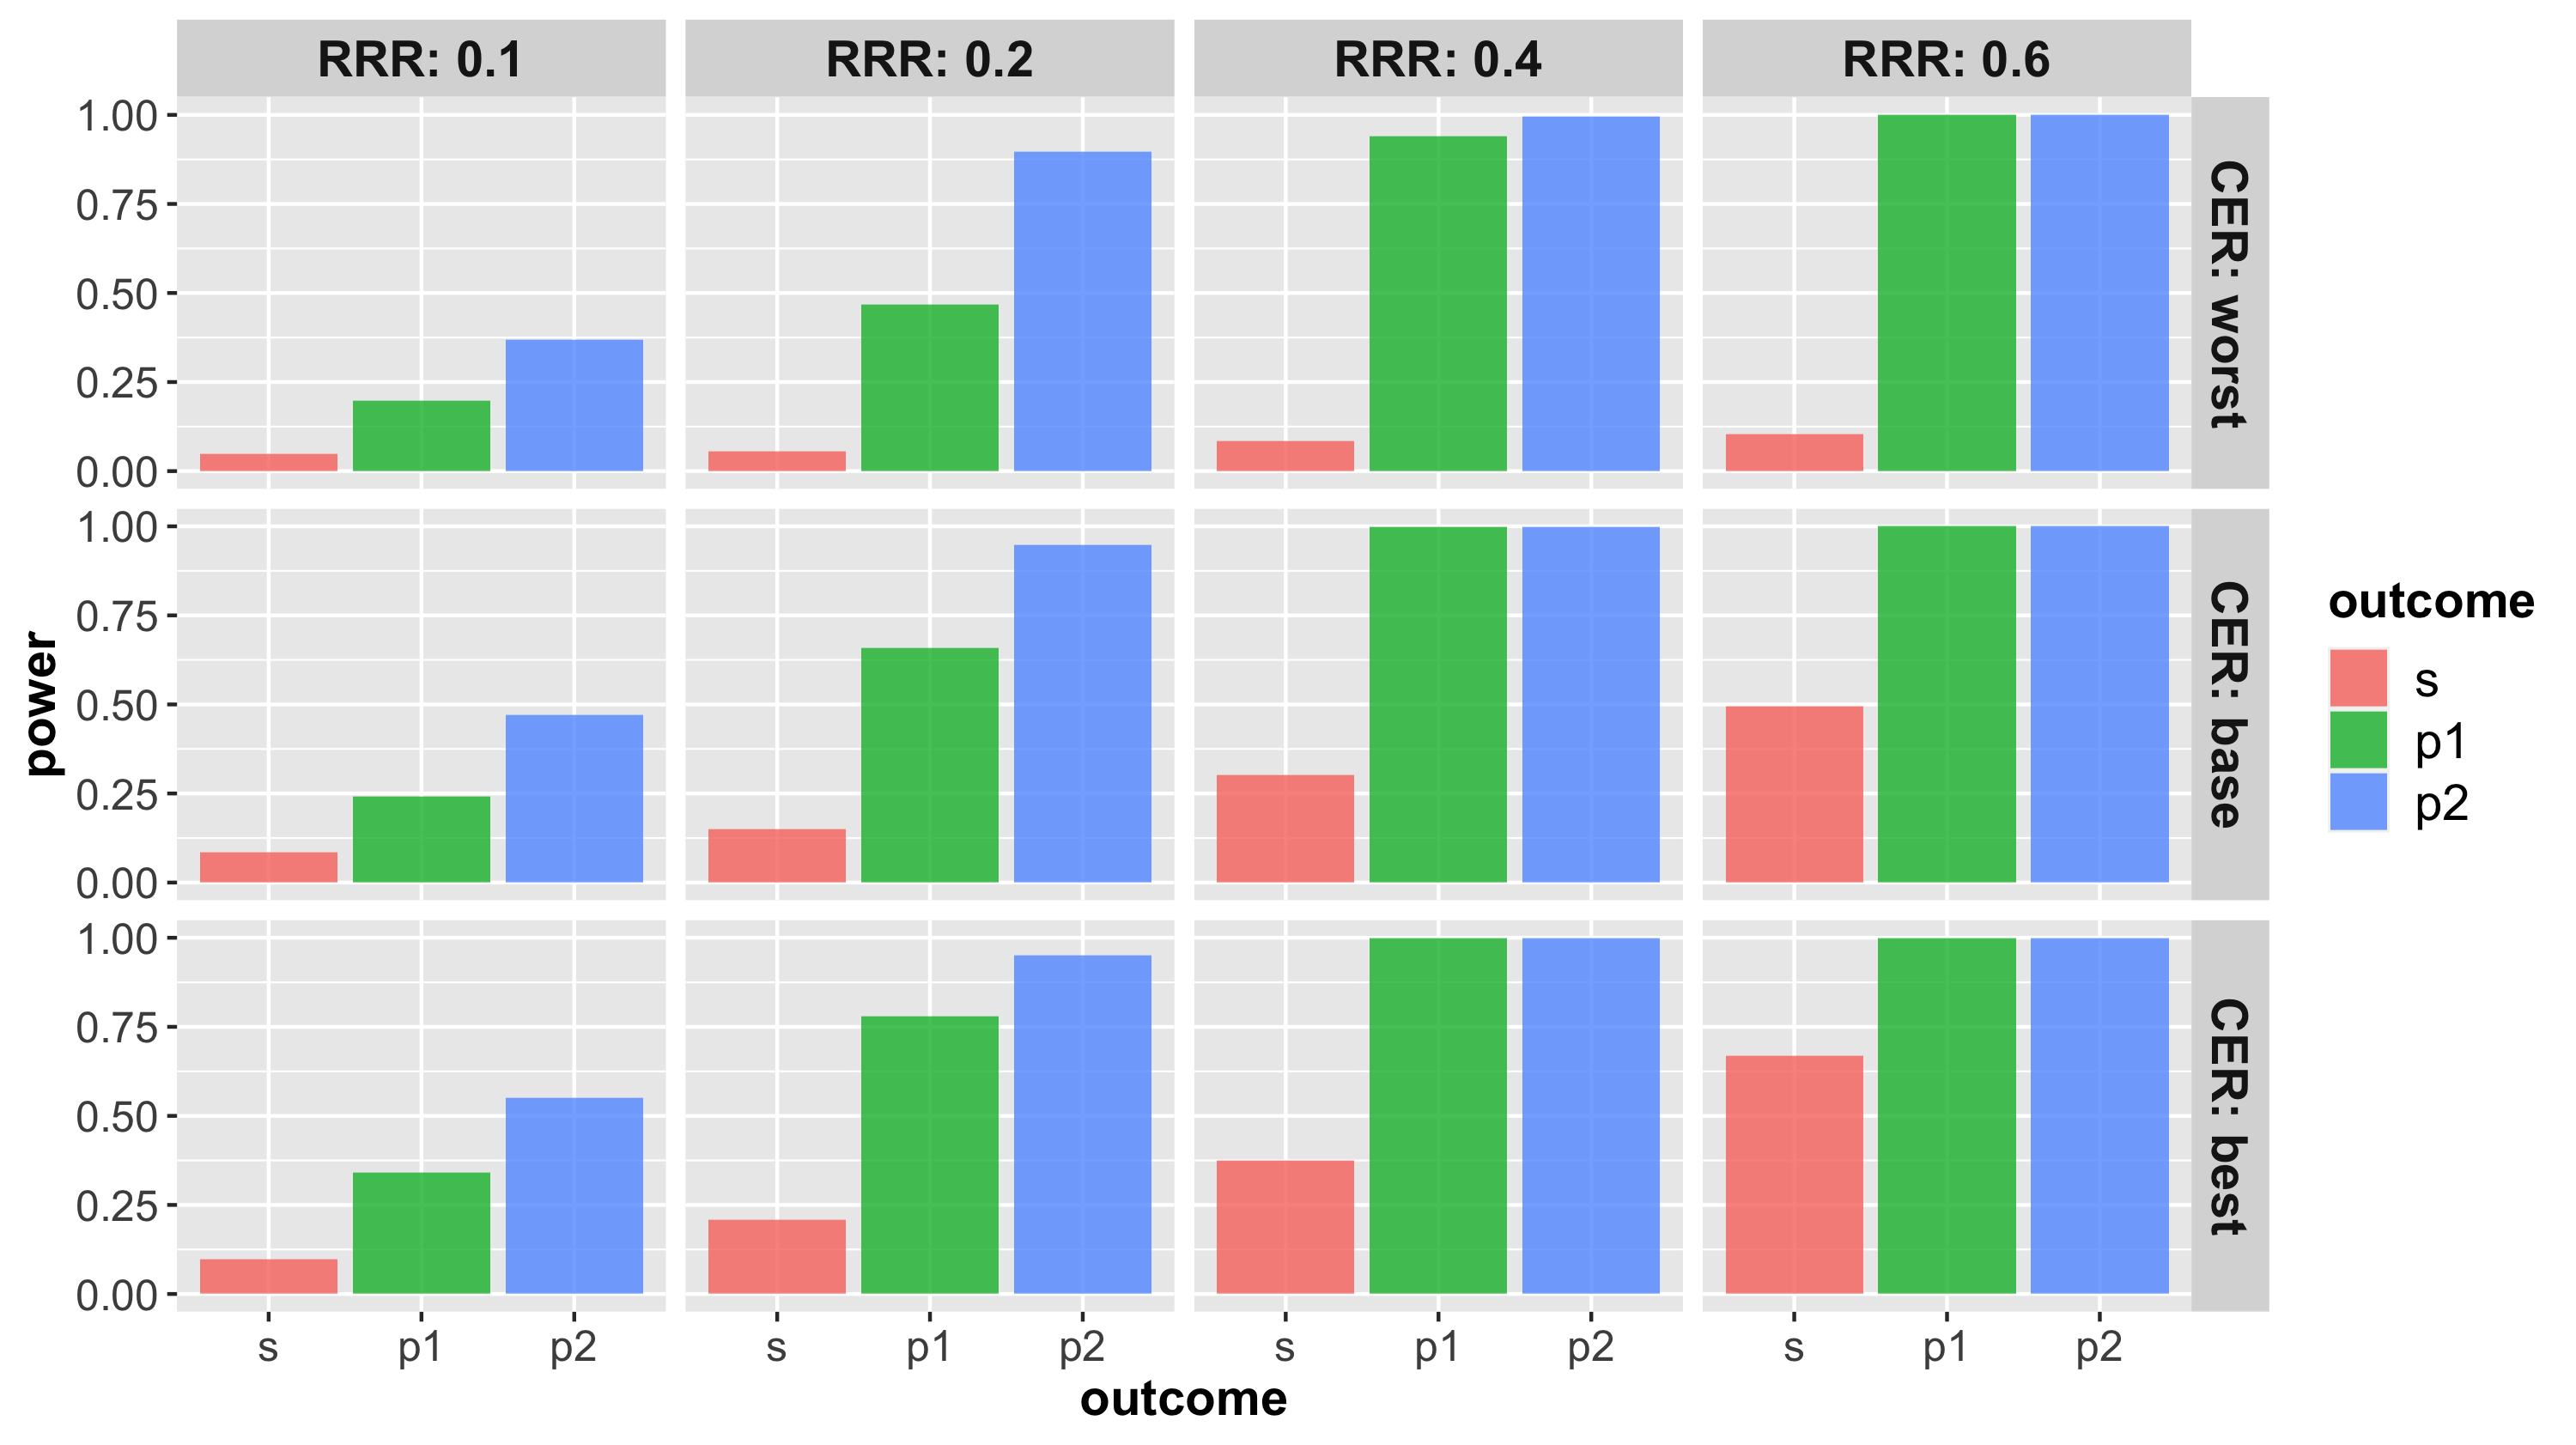
\includegraphics{../p1_plots/batch_size_nb_3000/power_p1.png}
\end{figure}

\hypertarget{expected-sample-size-2}{%
\subparagraph{Expected Sample Size}\label{expected-sample-size-2}}

\begin{figure}
  \caption{Expected sample size at trial termination. Results by control event scenarios are presented by rows. Results
  by relative risk reductions are presented by columns. Results by futility thresholds are presented by the color of the bars (see legend).}
  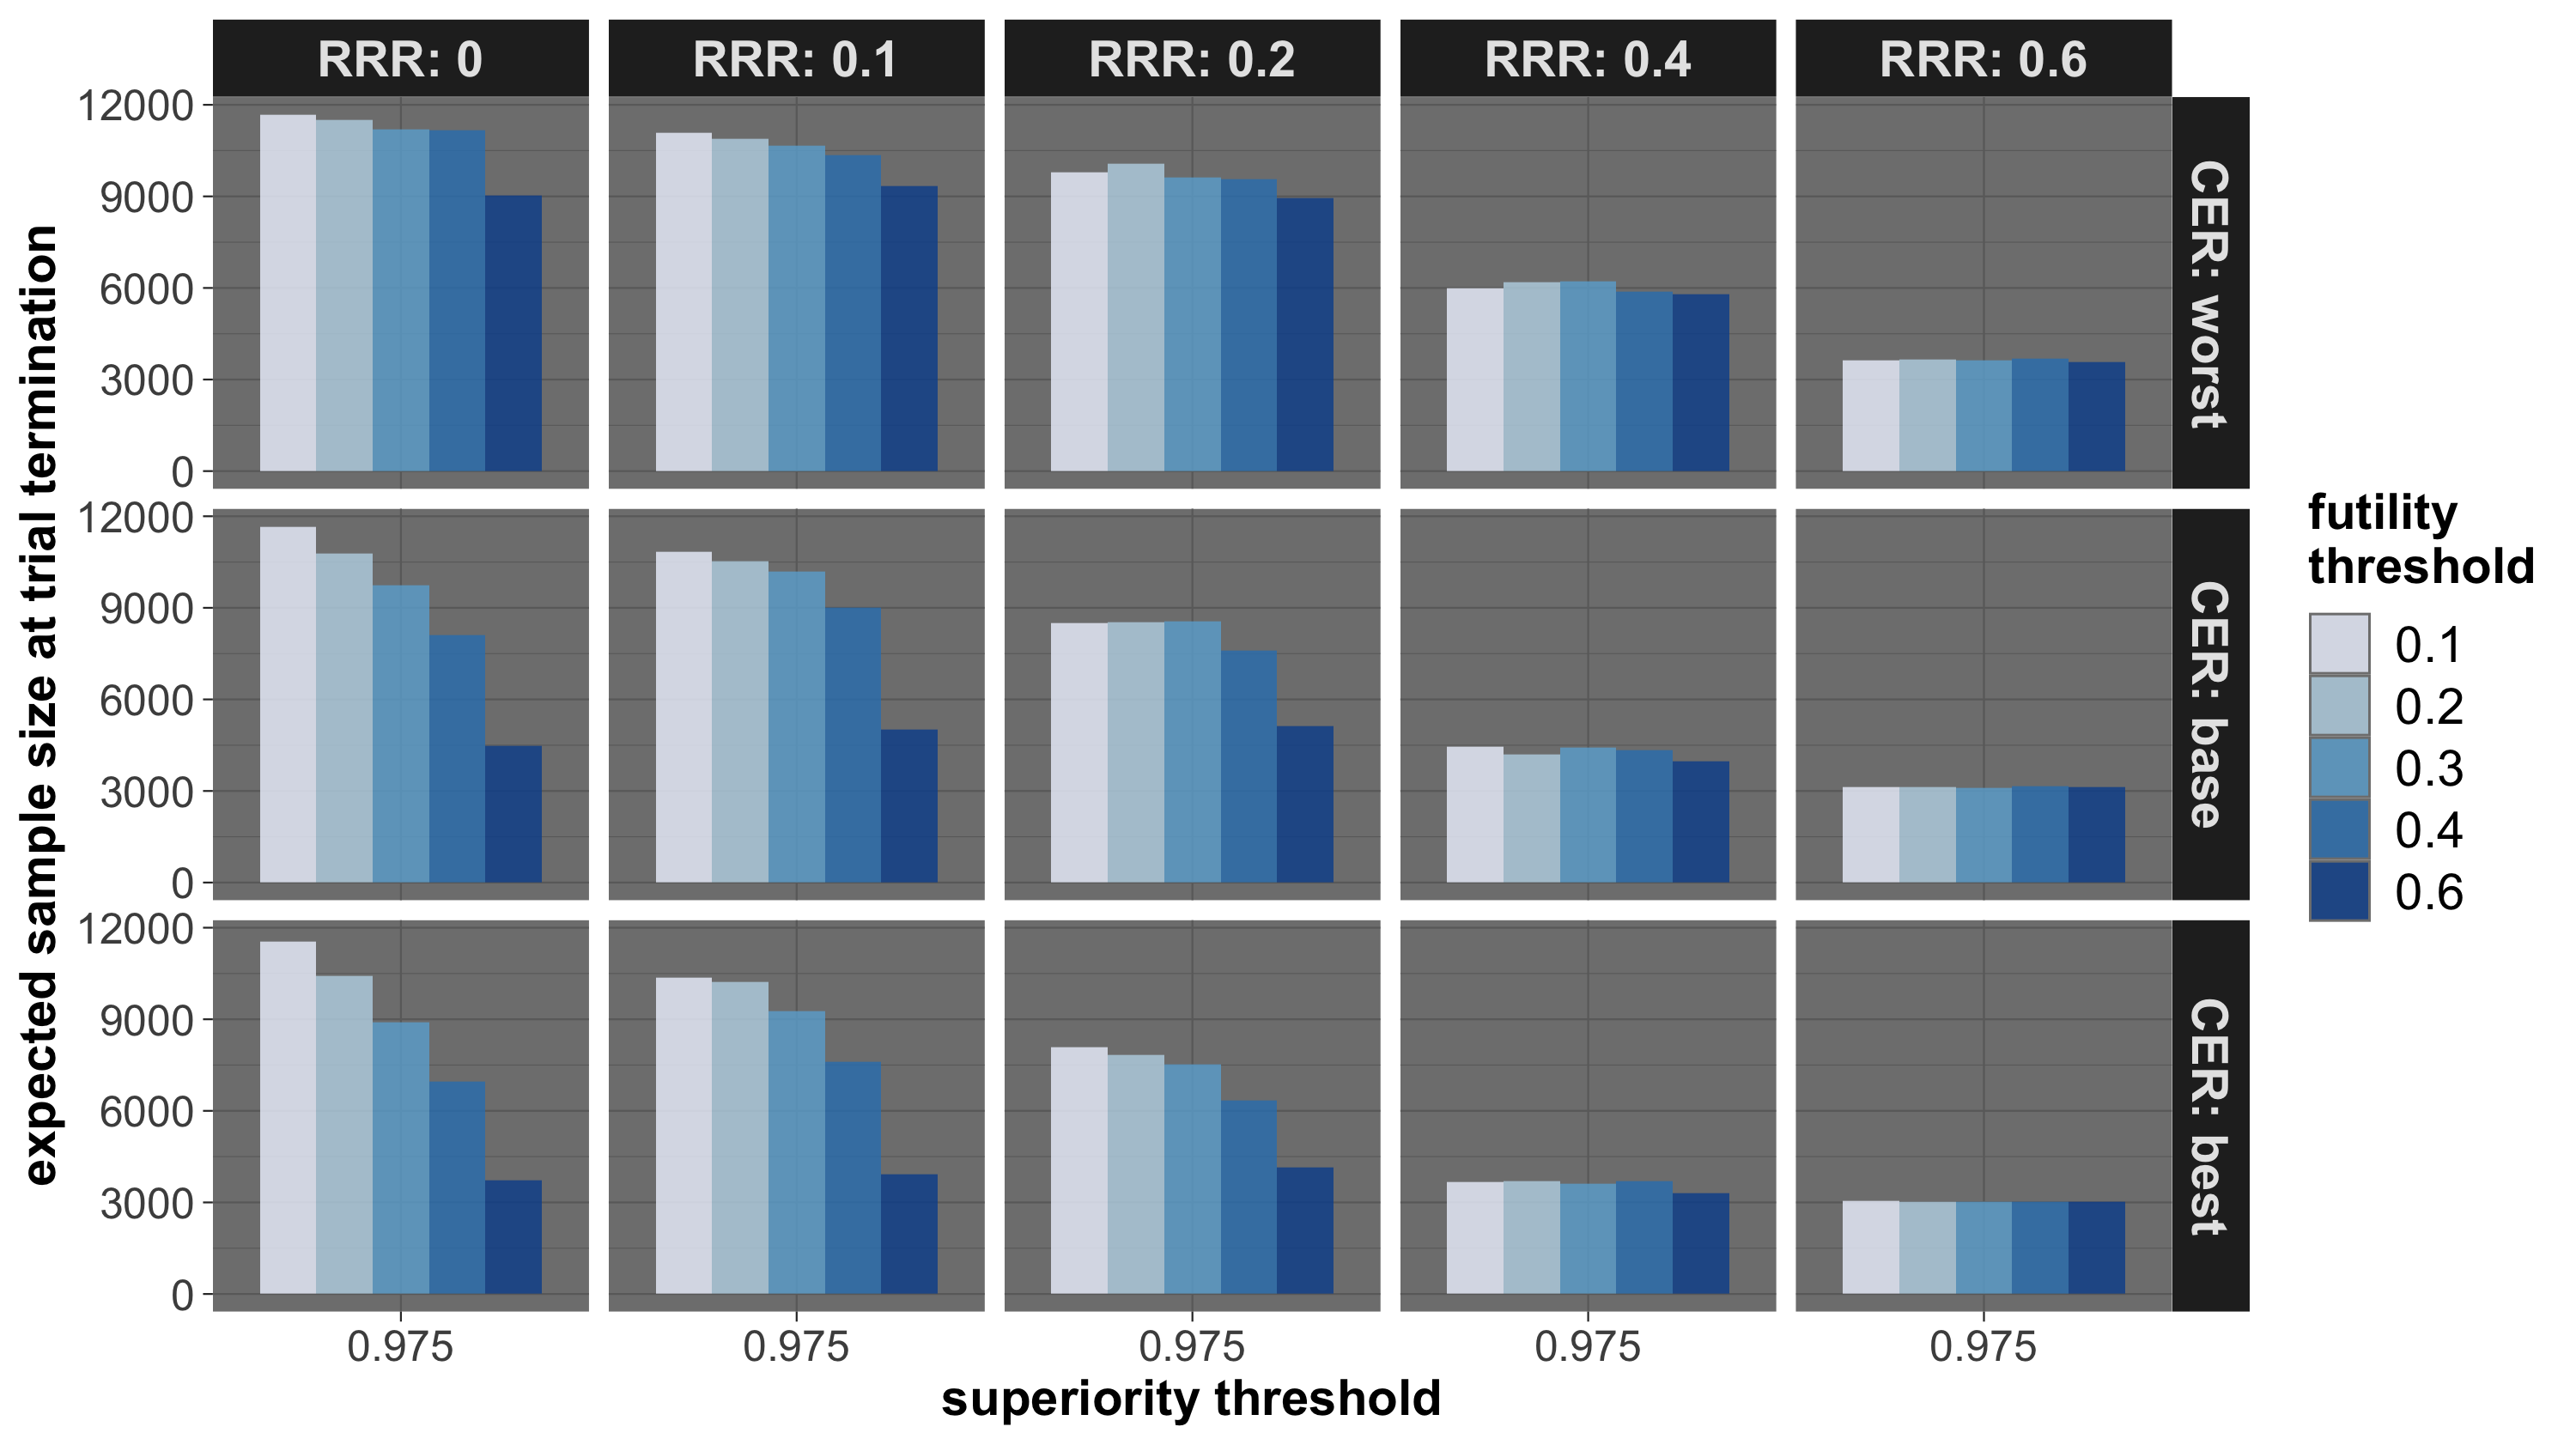
\includegraphics{../p1_plots/batch_size_nb_3000/exp_sample_size_p1.png}
\end{figure}

\hypertarget{probability-of-reaching-maximum-sample-size-2}{%
\paragraph{Probability of Reaching Maximum Sample
Size}\label{probability-of-reaching-maximum-sample-size-2}}

\begin{figure}
  \caption{Probability of reaching maximum sample size for the three control event rates (CER – rows), four relative
  risk reductions (RRR – columns), and three futility thresholds (legend).}
  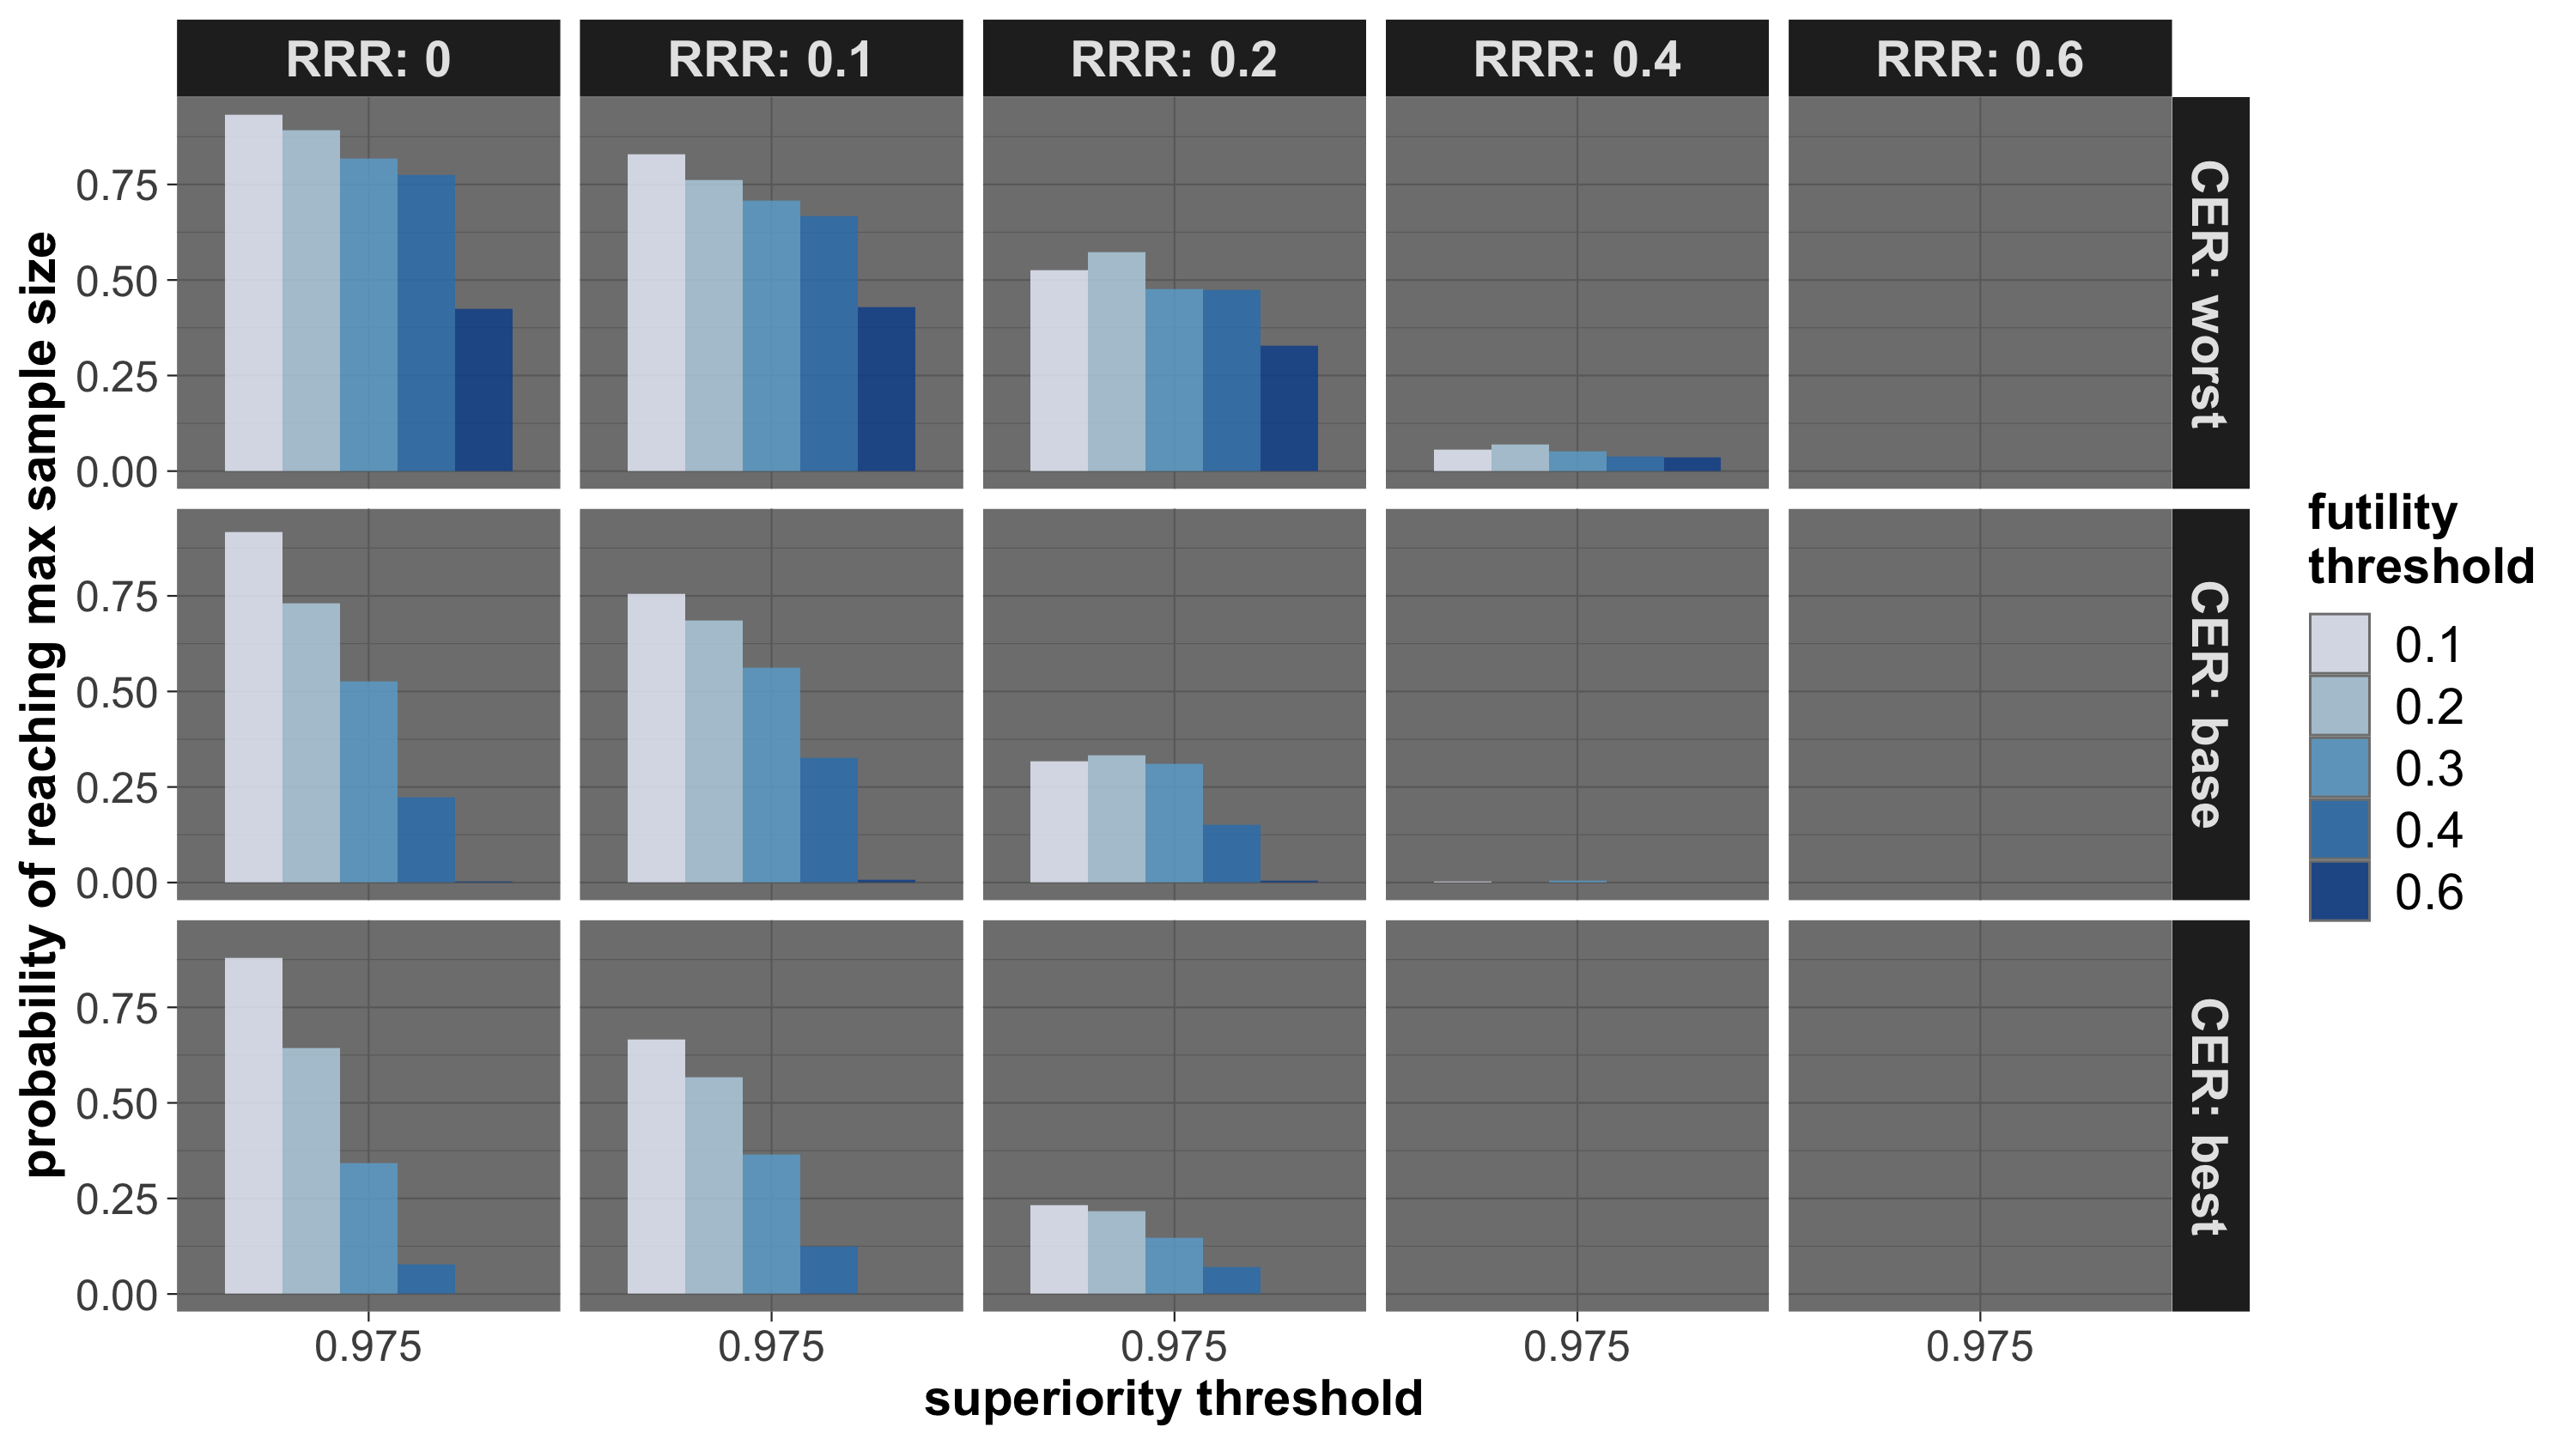
\includegraphics{../p1_plots/batch_size_nb_3000/prob_reach_max_size_p1.png}
\end{figure}

\hypertarget{probability-of-stopping-early-2}{%
\paragraph{Probability of Stopping
Early}\label{probability-of-stopping-early-2}}

\begin{figure}
  \caption{Probability of stopping early due to futility or superiority for the three control event rates (CER – rows),
  four relative risk reductions (RRR – columns), three superiority thresholds (x axis) and three futility thresholds
  (legend).}
  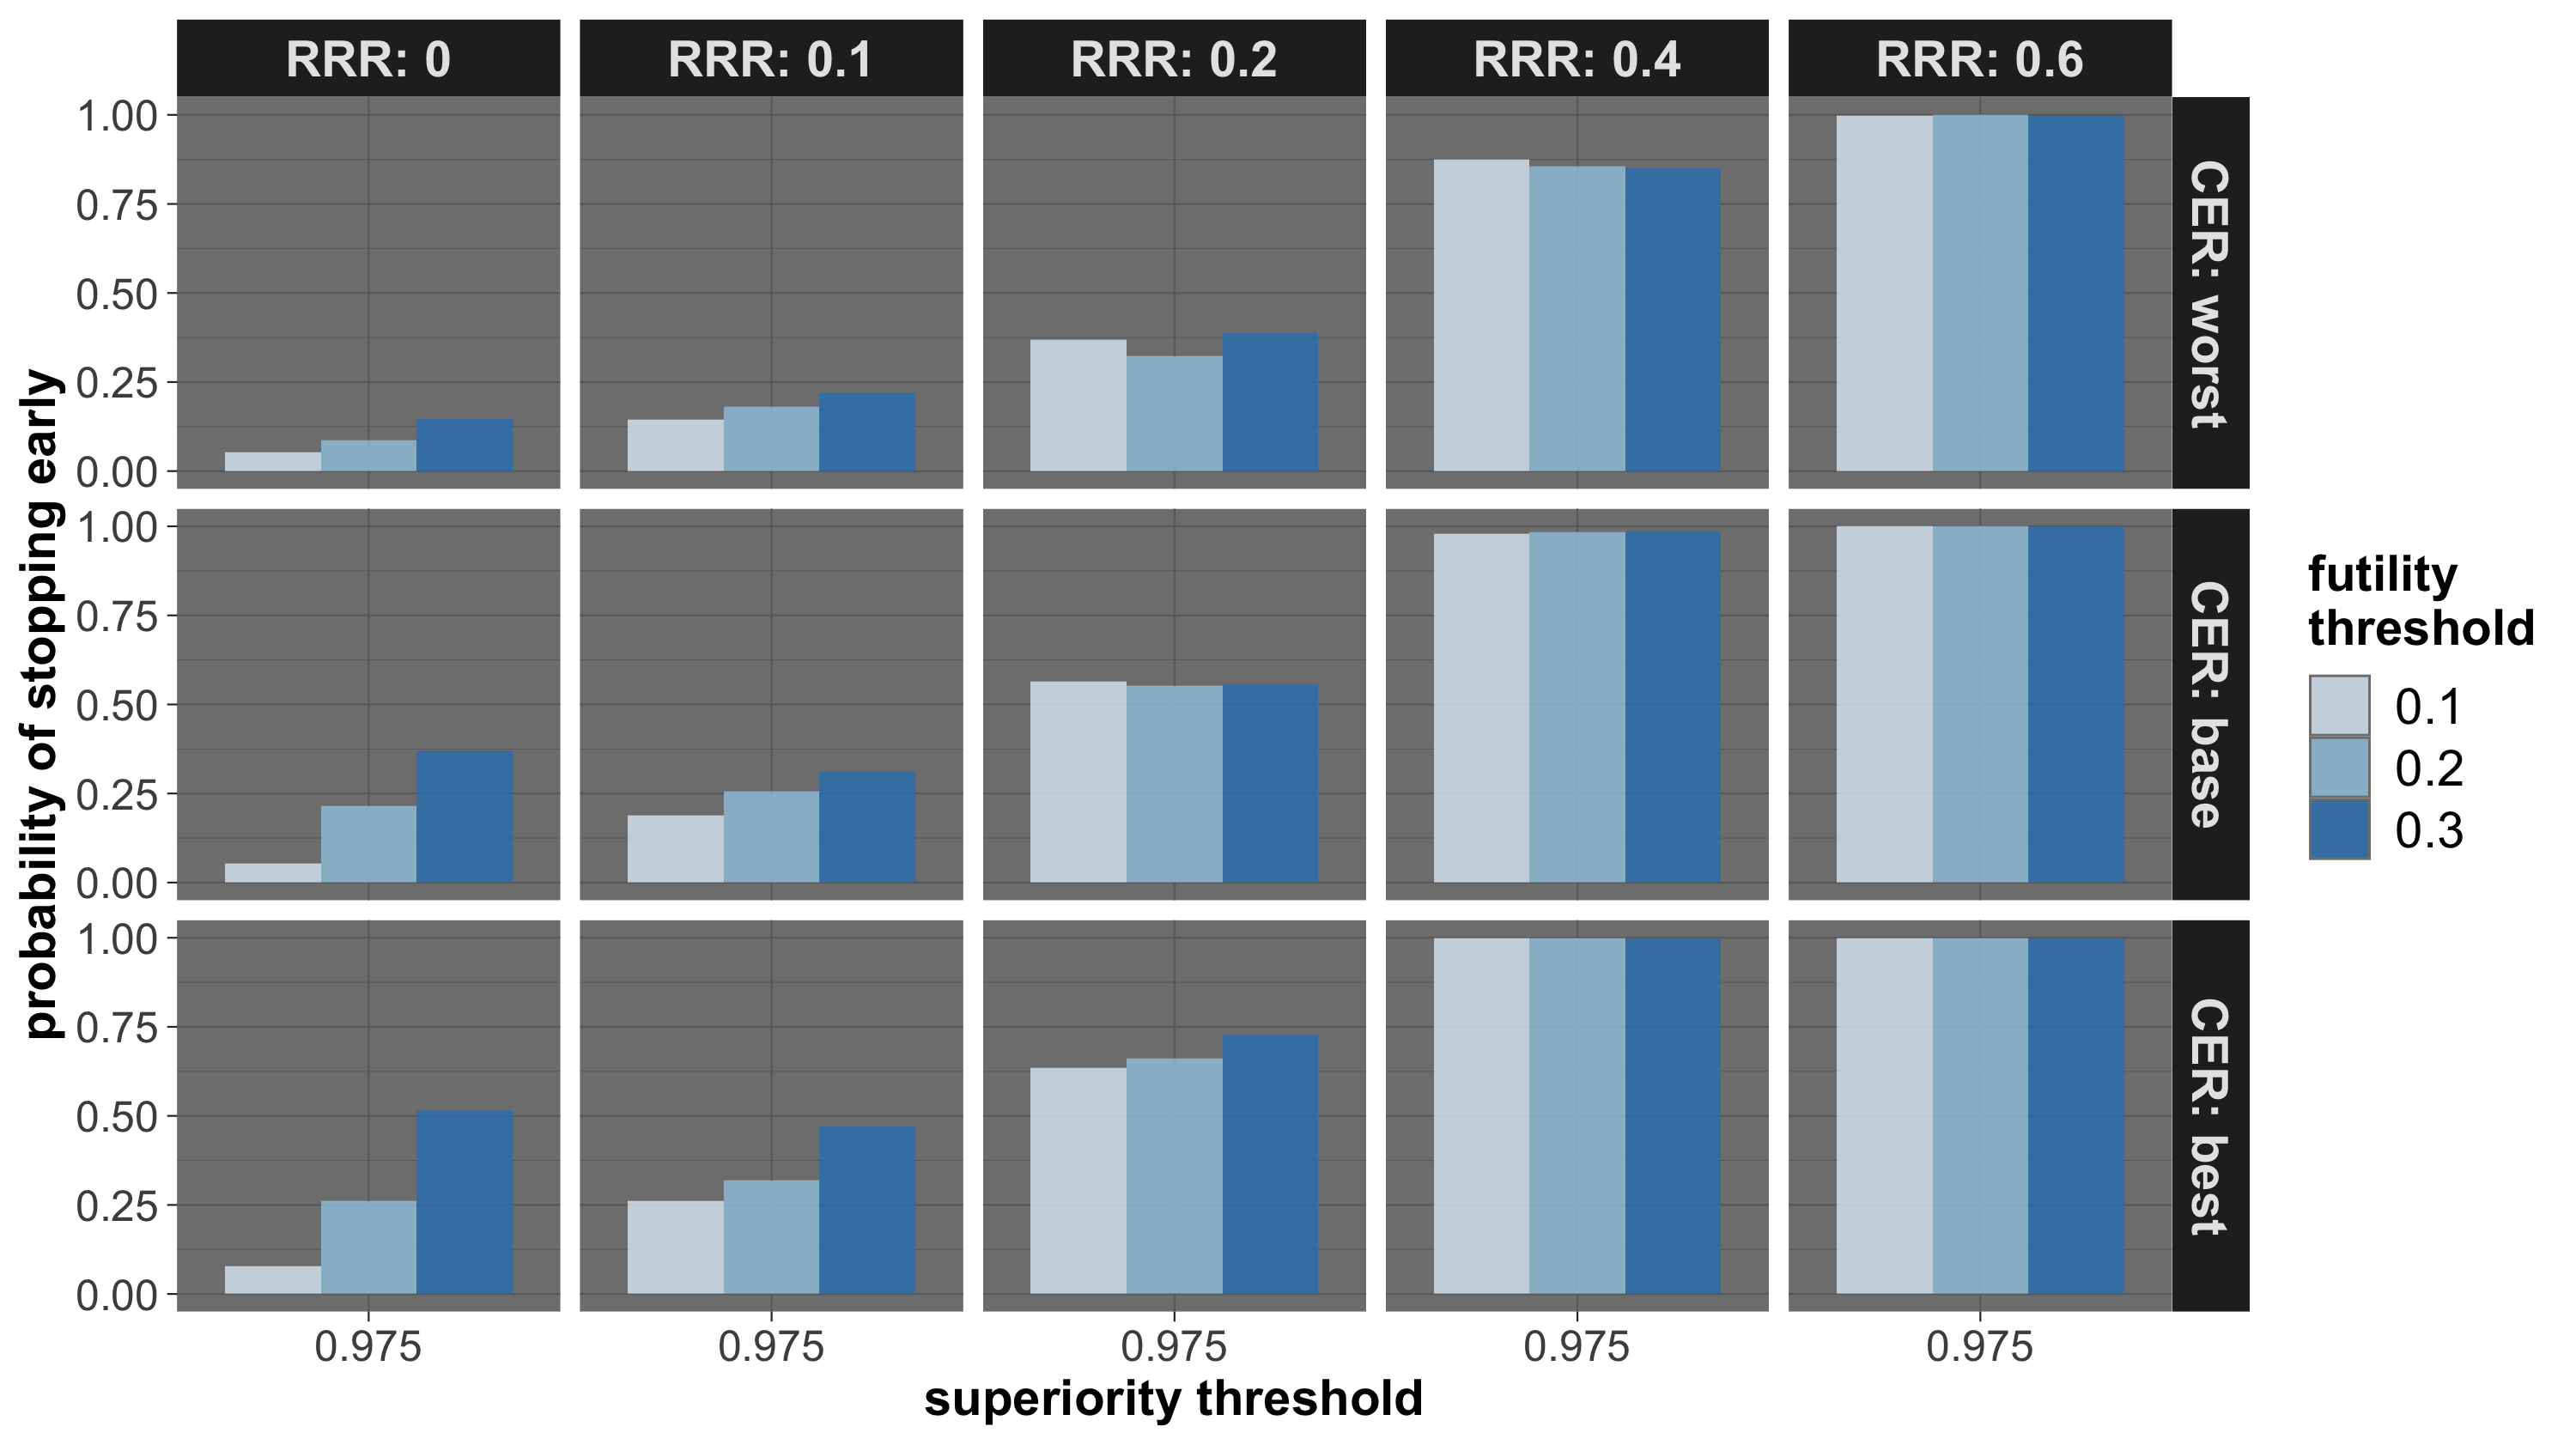
\includegraphics{../p1_plots/batch_size_nb_3000/prob_stop_early_p1.png}
\end{figure}

\begin{figure}
\centering
  \caption{Probability of stopping early due to futility, and stopping early due to superiority. Stopping probabilities
  are presented for the three control event rates (CER – rows), four relative risk reductions (RRR – columns), and three futility thresholds (legend).}
  \label{fig:fig}
  \begin{subfigure}{0.8\textwidth}
    \centering
    \caption{}
    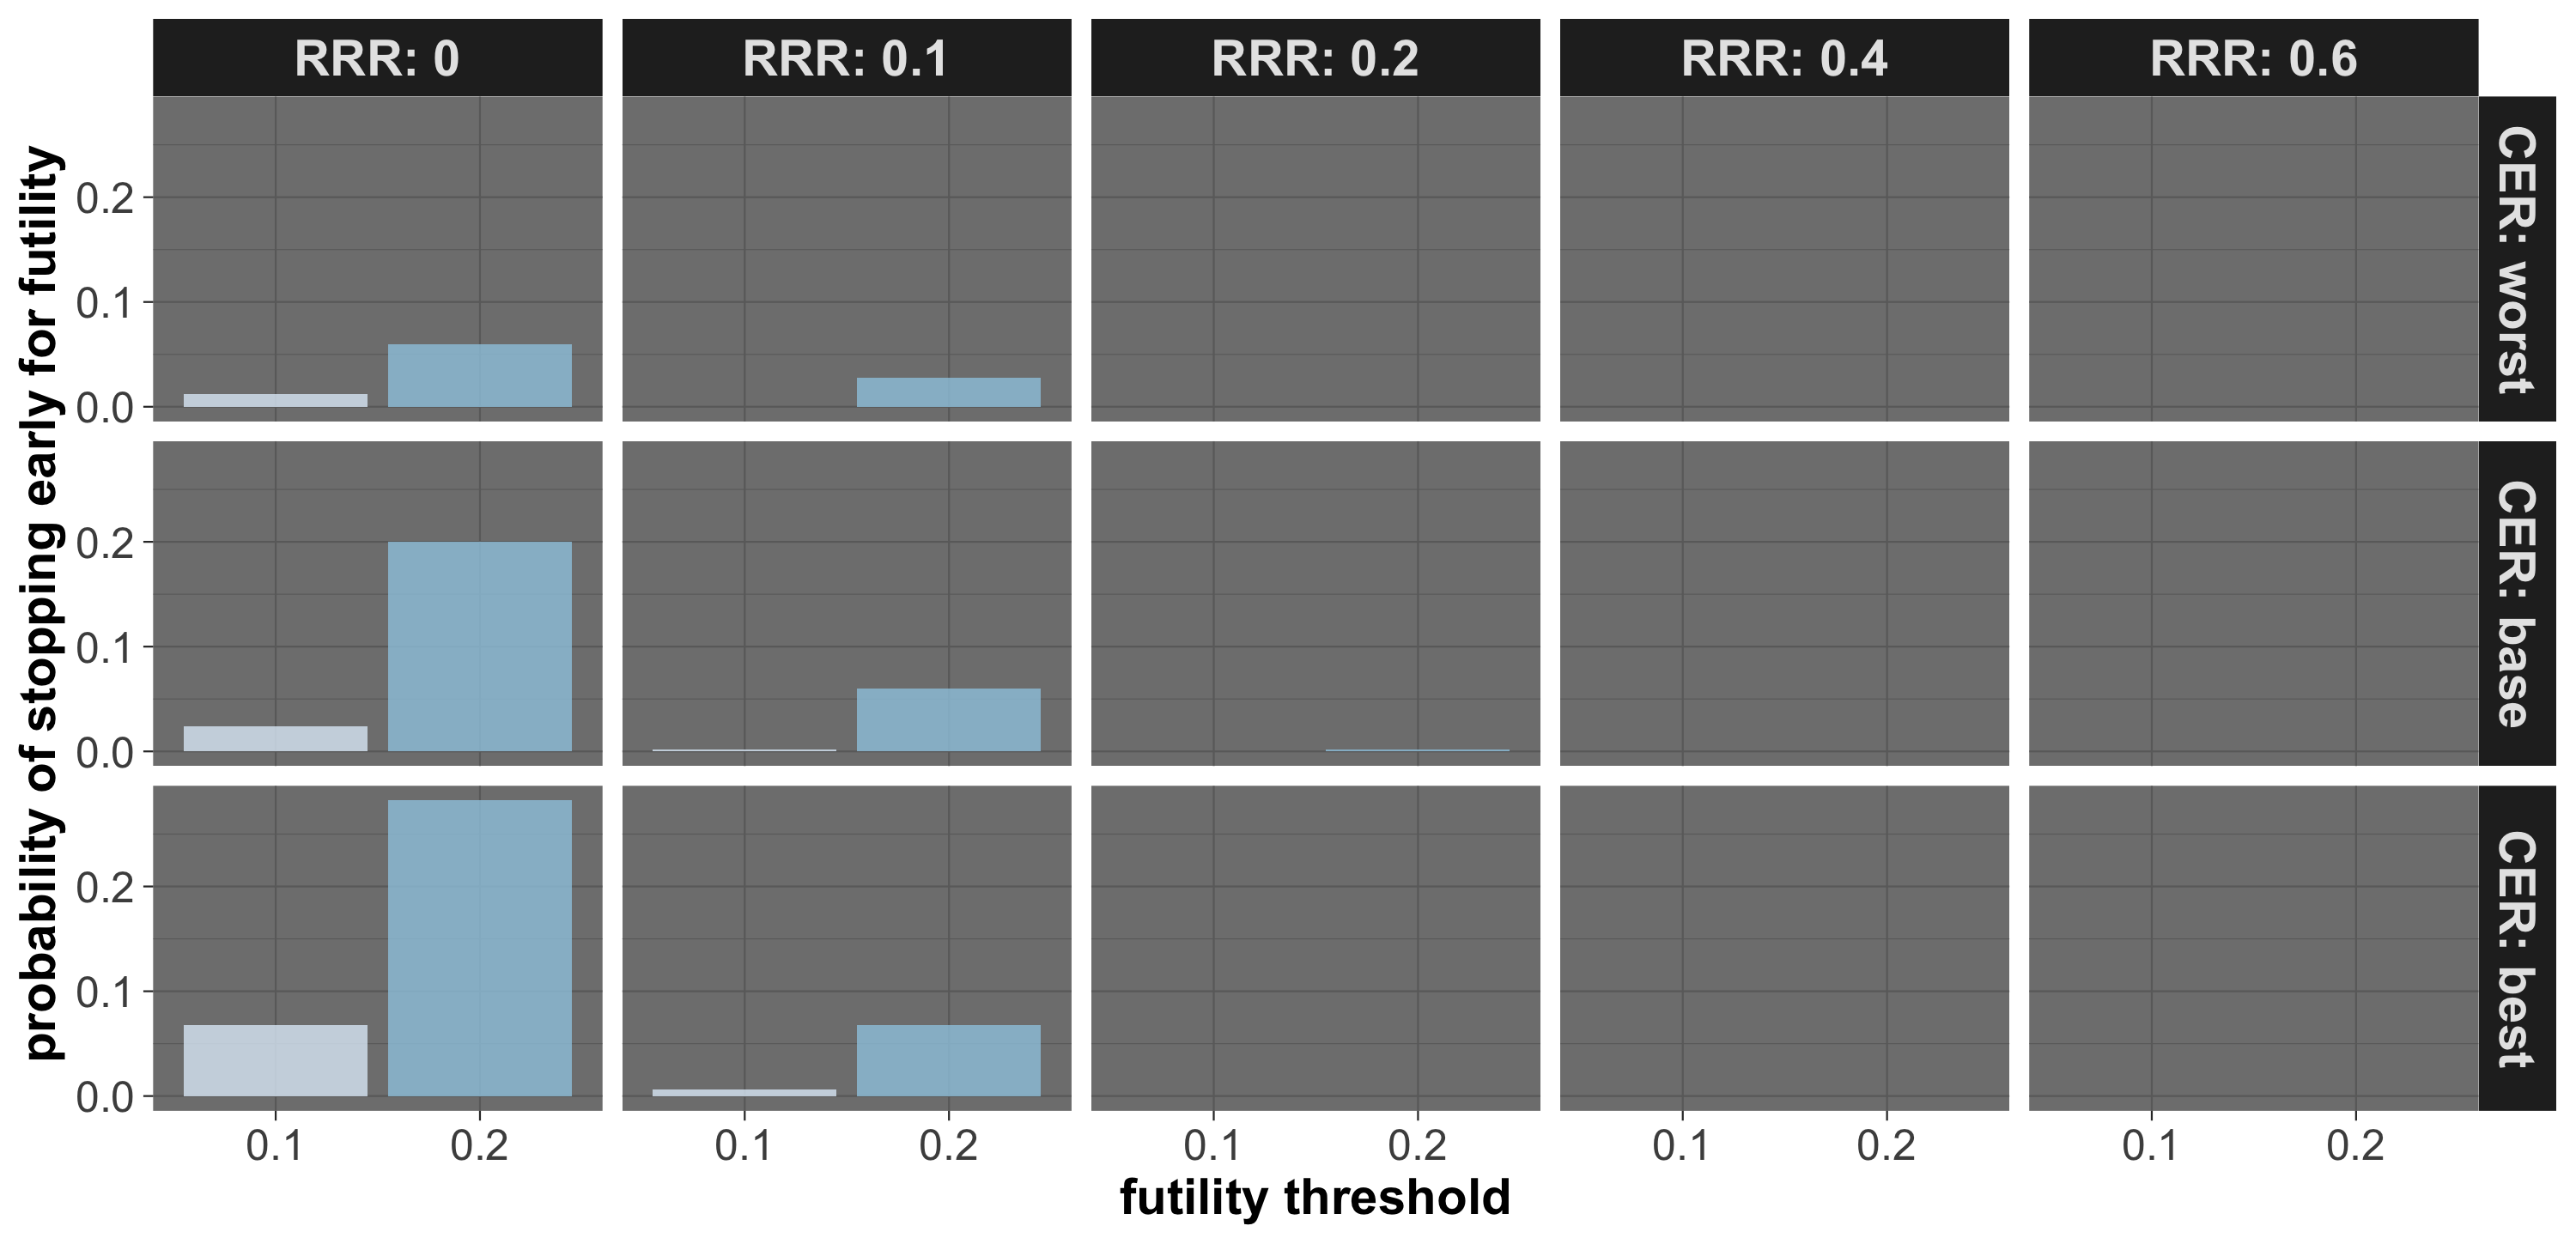
\includegraphics{../p1_plots/batch_size_nb_3000/prob_stop_early_fut_p1.png}
  \end{subfigure}
  \begin{subfigure}{0.8\textwidth}
    \centering
    \caption{}
    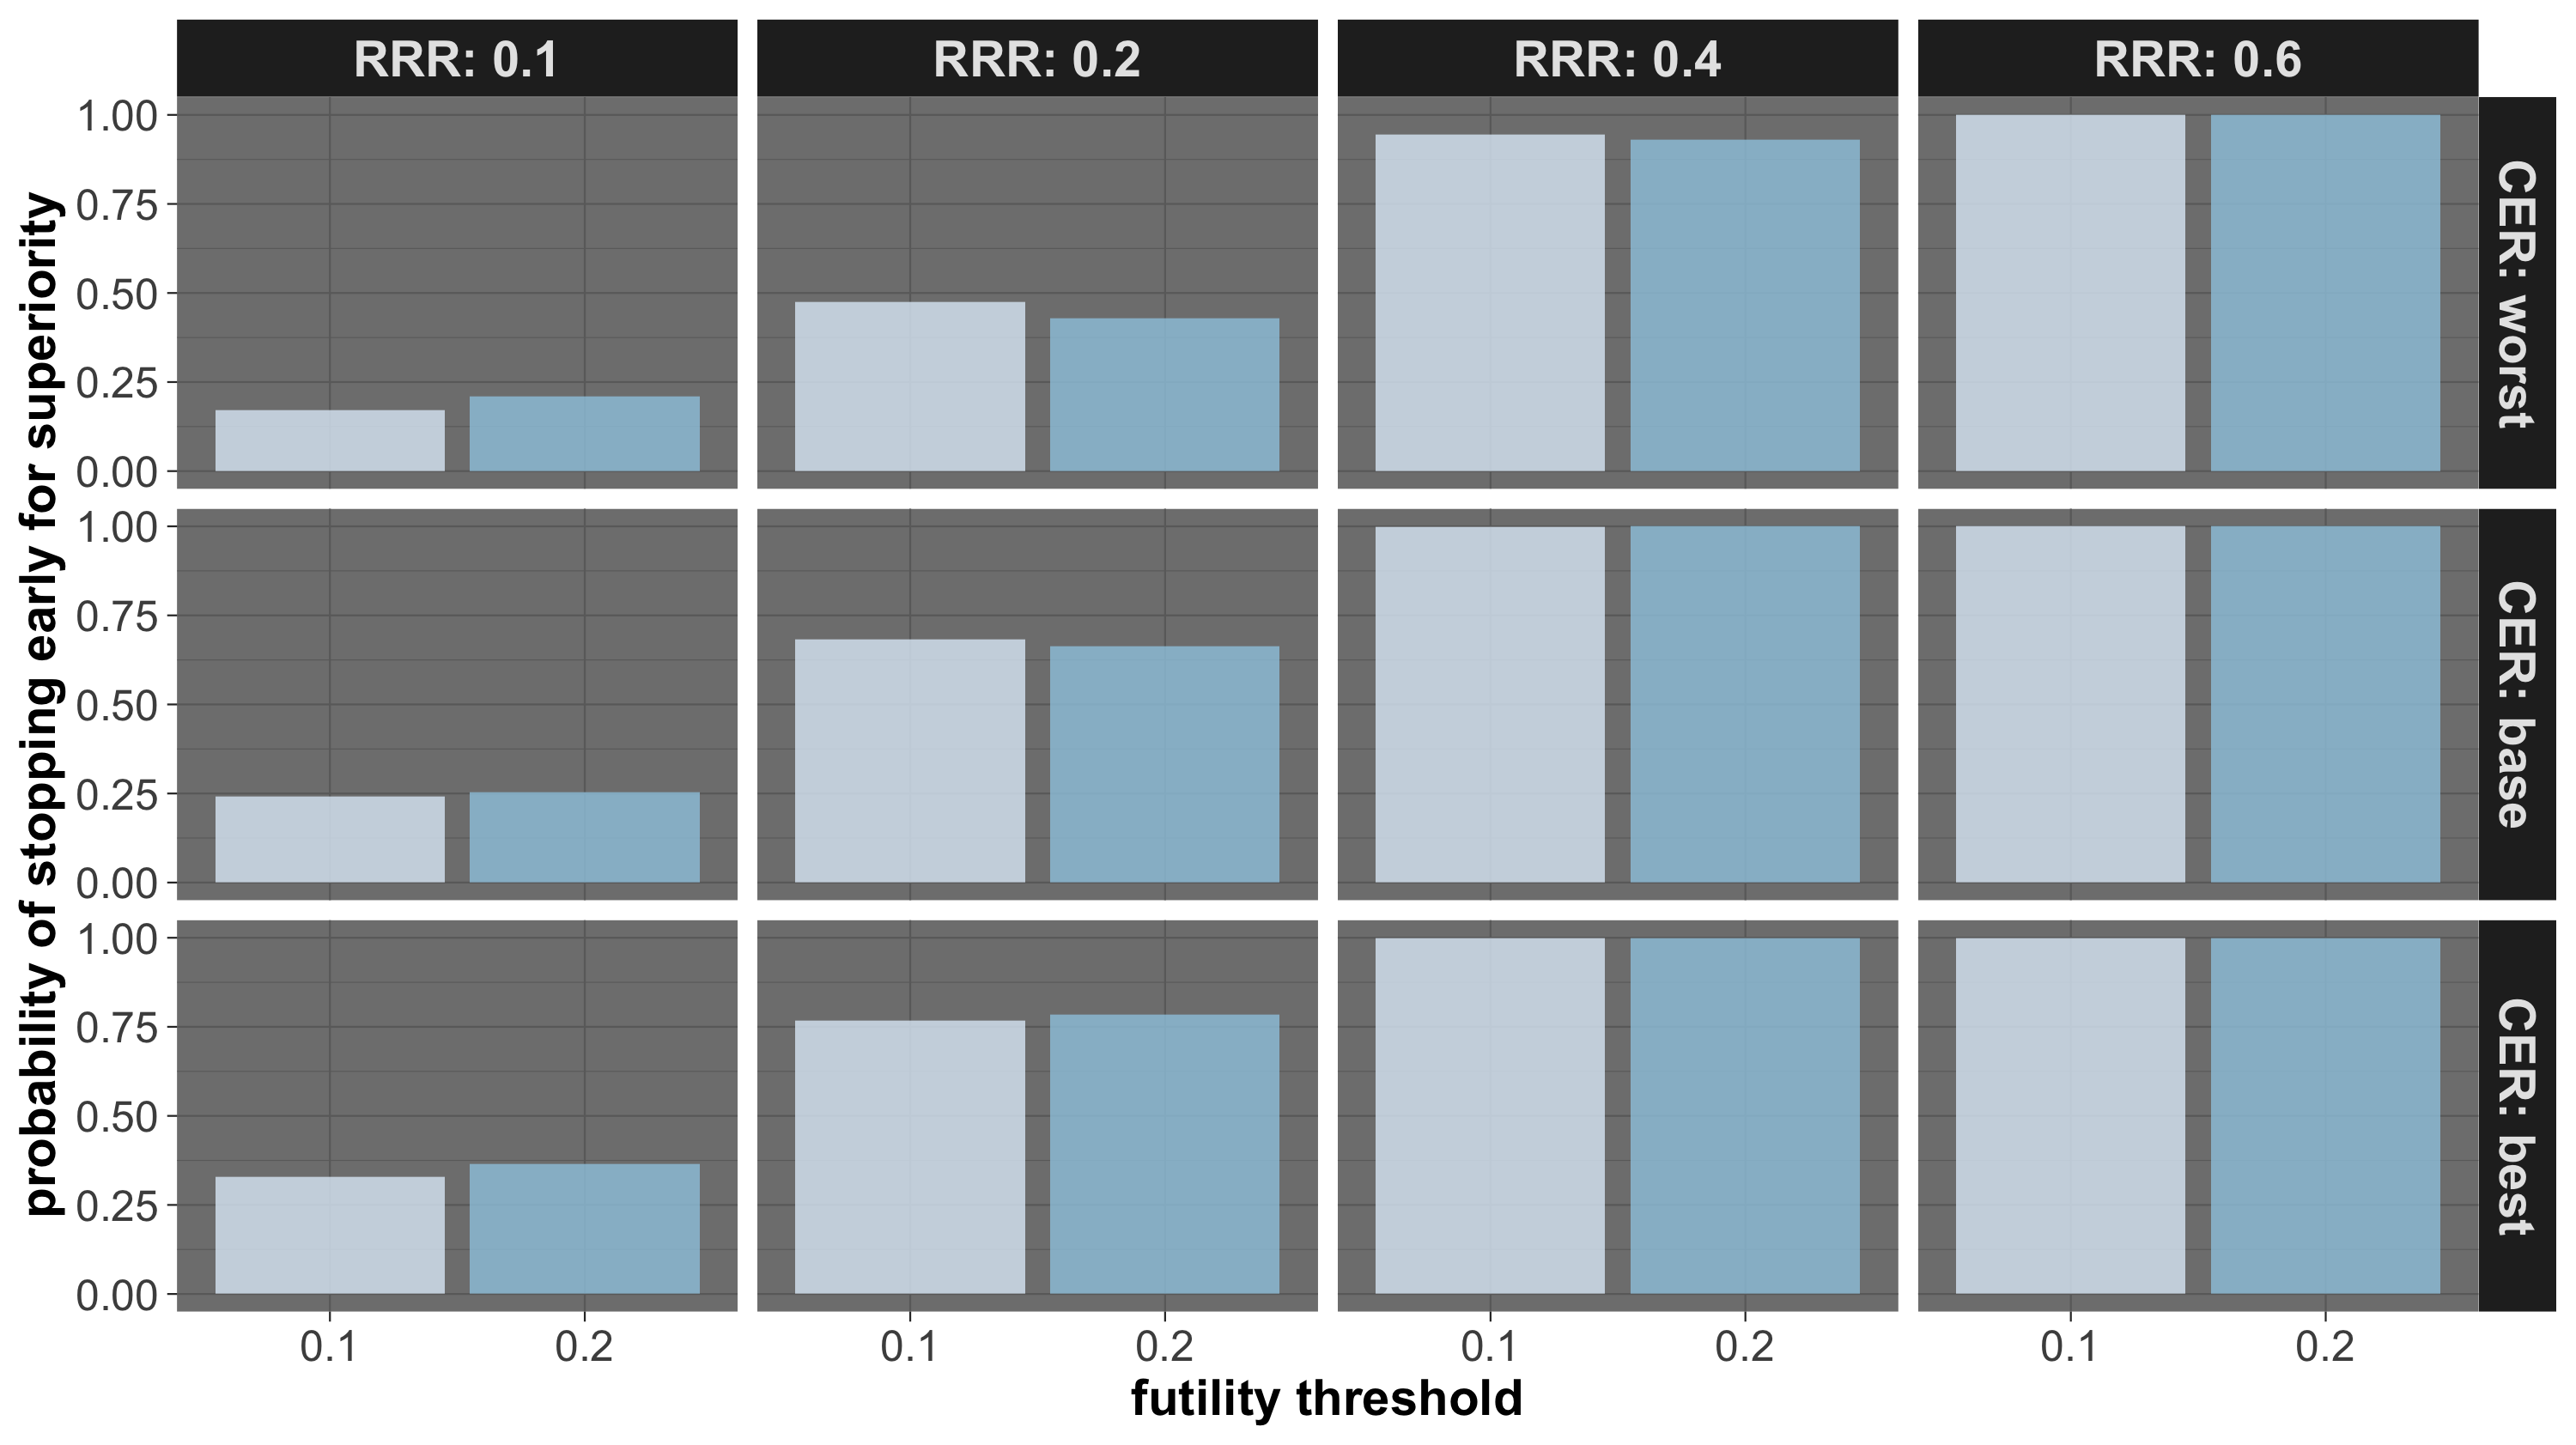
\includegraphics{../p1_plots/batch_size_nb_3000/prob_stop_early_sup_p1.png}
  \end{subfigure}
\end{figure}

\hypertarget{p-values-at-trial-termination-when-a-true-effect-exists-2}{%
\paragraph{P-values at trial termination when a true effect
exists}\label{p-values-at-trial-termination-when-a-true-effect-exists-2}}

\begin{figure}
  \caption{Overall probability at trial termination that the p-value (from Fisher’s exact test) at termination of the
  trial is below 5\%, between 5\% and 10\% and greater than 10\%. The rows represent the three control even rate scenarios
  and the three columns present the three relative risk reduction scenarios.}
  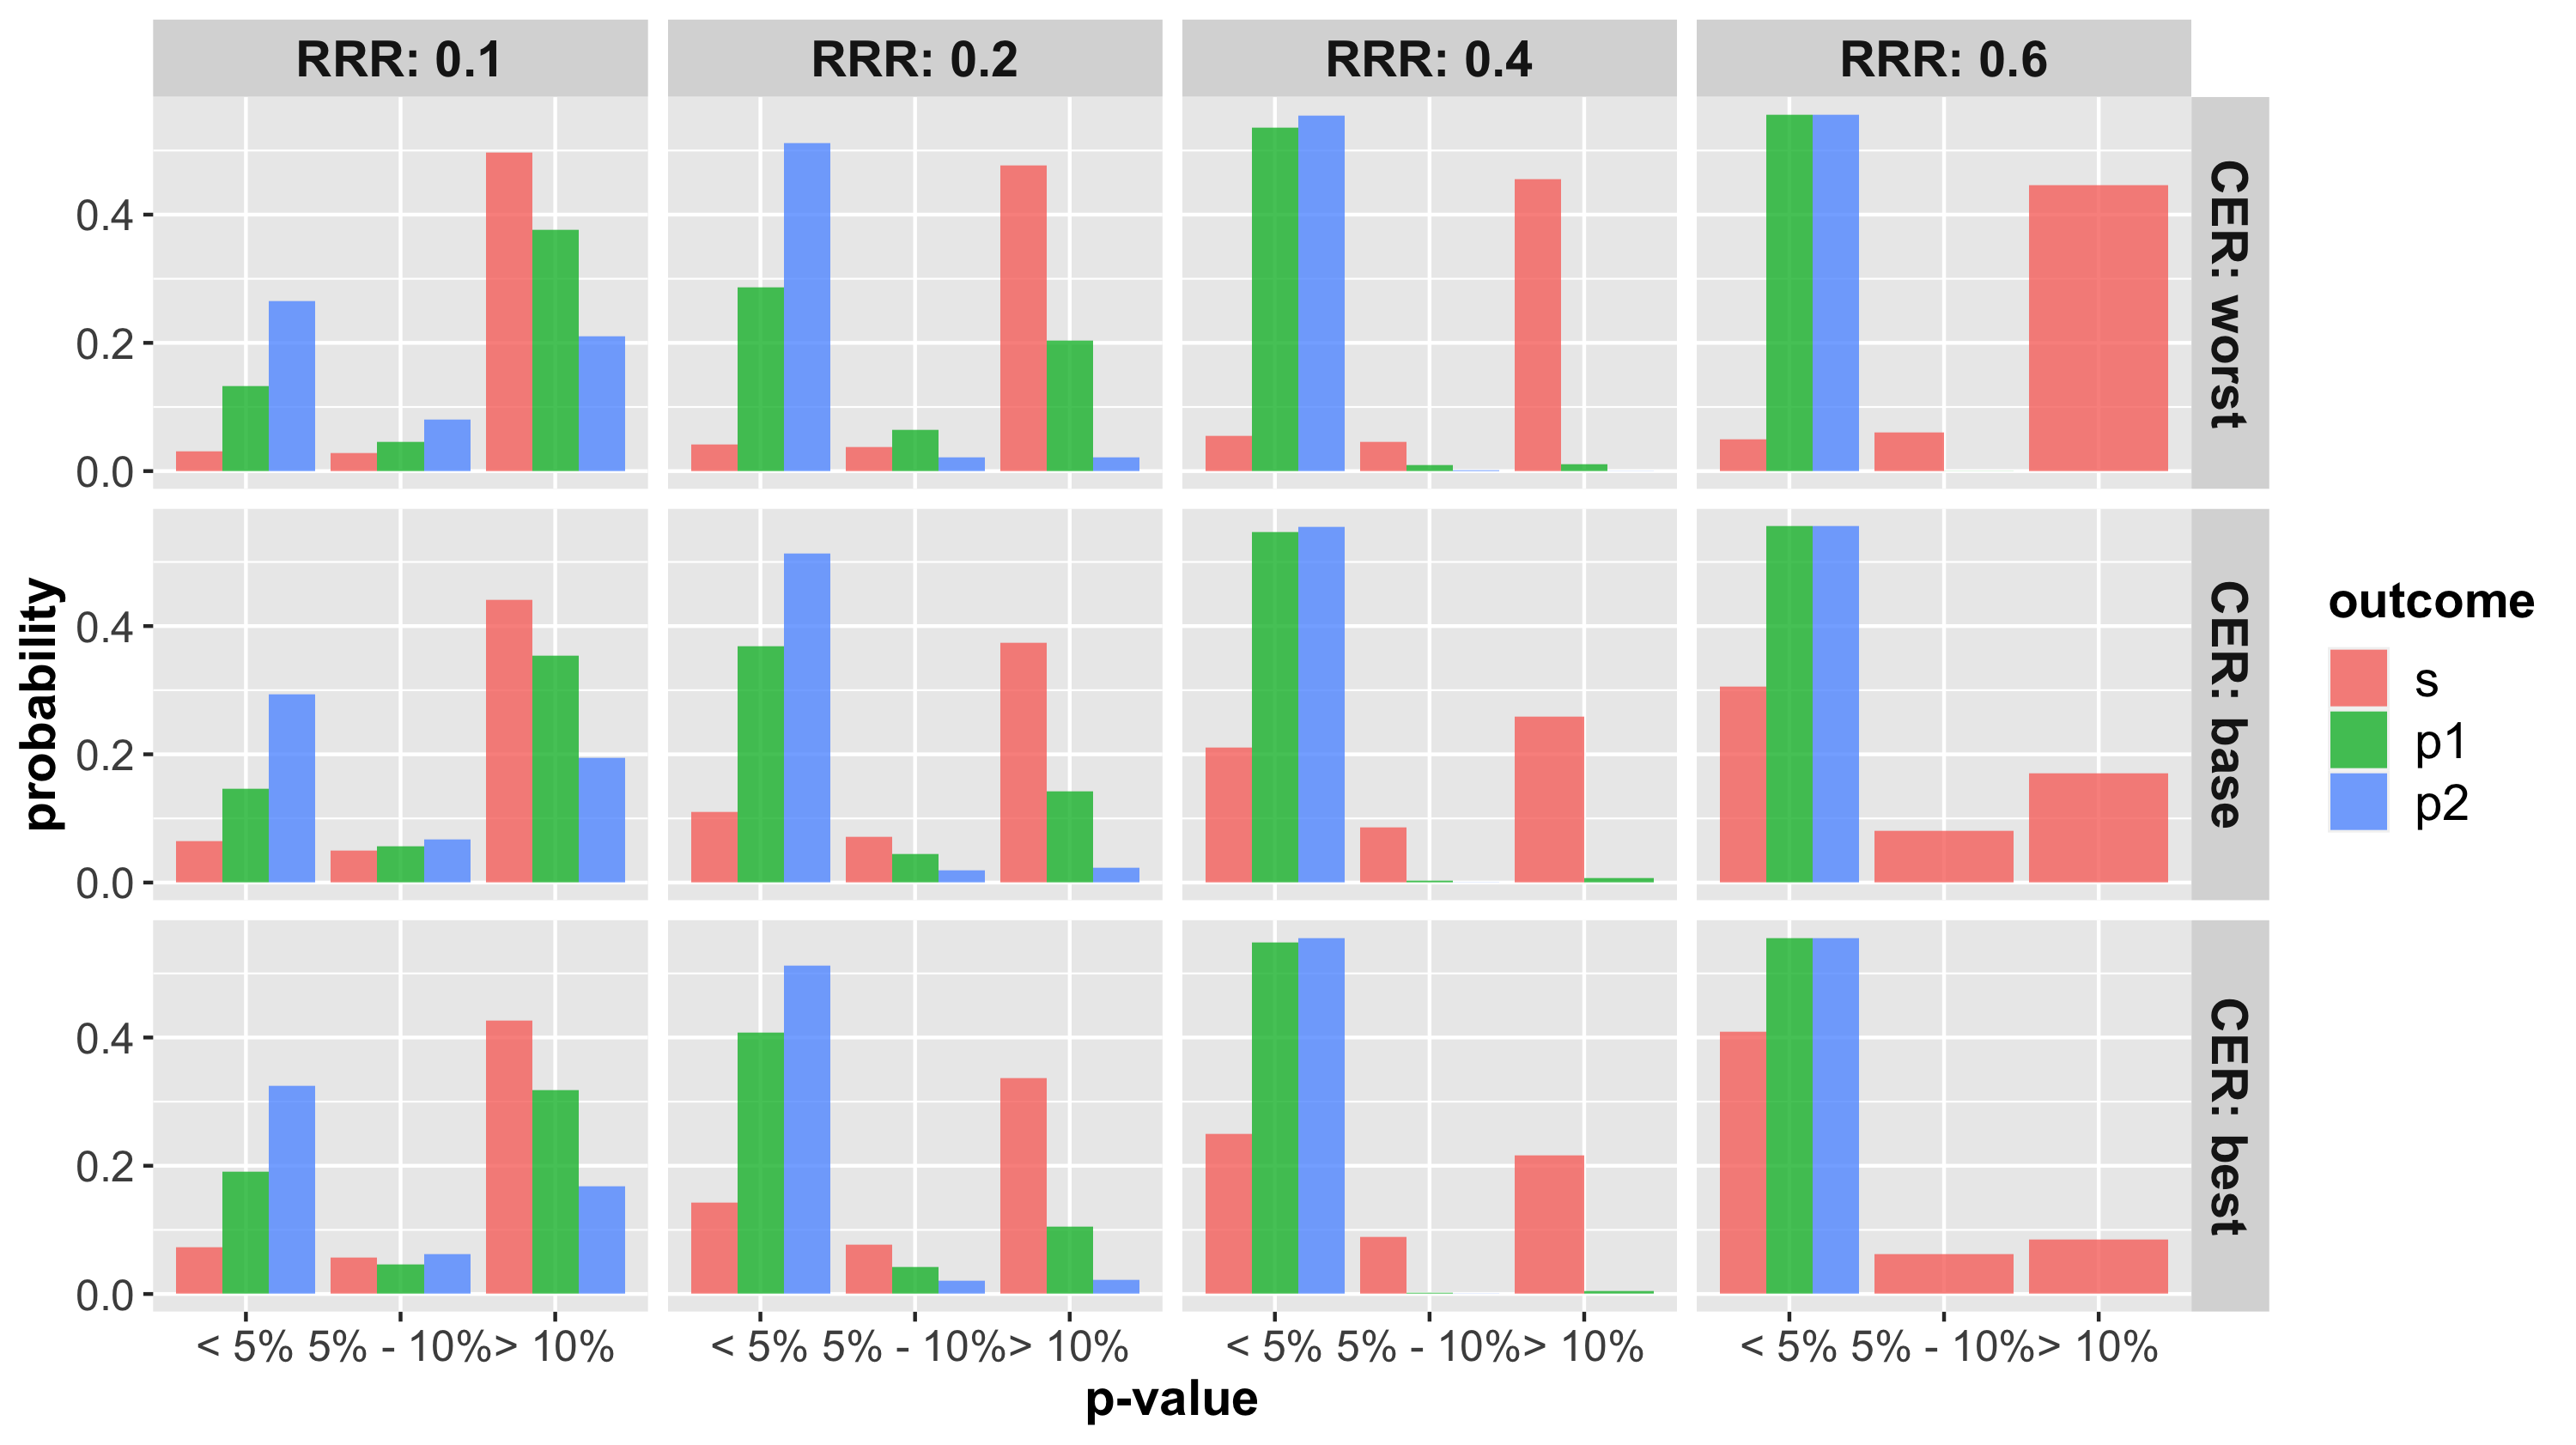
\includegraphics{../p1_plots/batch_size_nb_3000/pvalue_p1.png}
\end{figure}

\begin{figure}
\centering
  \caption{Probability that the p-value (from Fisher’s exact test) at termination of the trial is below 5\%, between 5\%
  and 10\% and greater than 10\% for cases where trial was (a) stopped for futility; (b) stopped for superiority. The
  rows represent the three control even rate scenarios and the three columns present the three relative risk reduction
  scenarios. Note: the denominator in each figure is the number of simulations (not the number of trials stopped for
  futility (a) or superiority (b), and thus, the proportions do not add up to 100\% within one figure. Further, (a) and
  (b) do not include simulations where the trial went to the max. allowed sample size. The bars should be interpreted
  with respect to the relative proportion that fit in each category.}
  \begin{subfigure}{0.8\textwidth}
    \centering
    \caption{}
    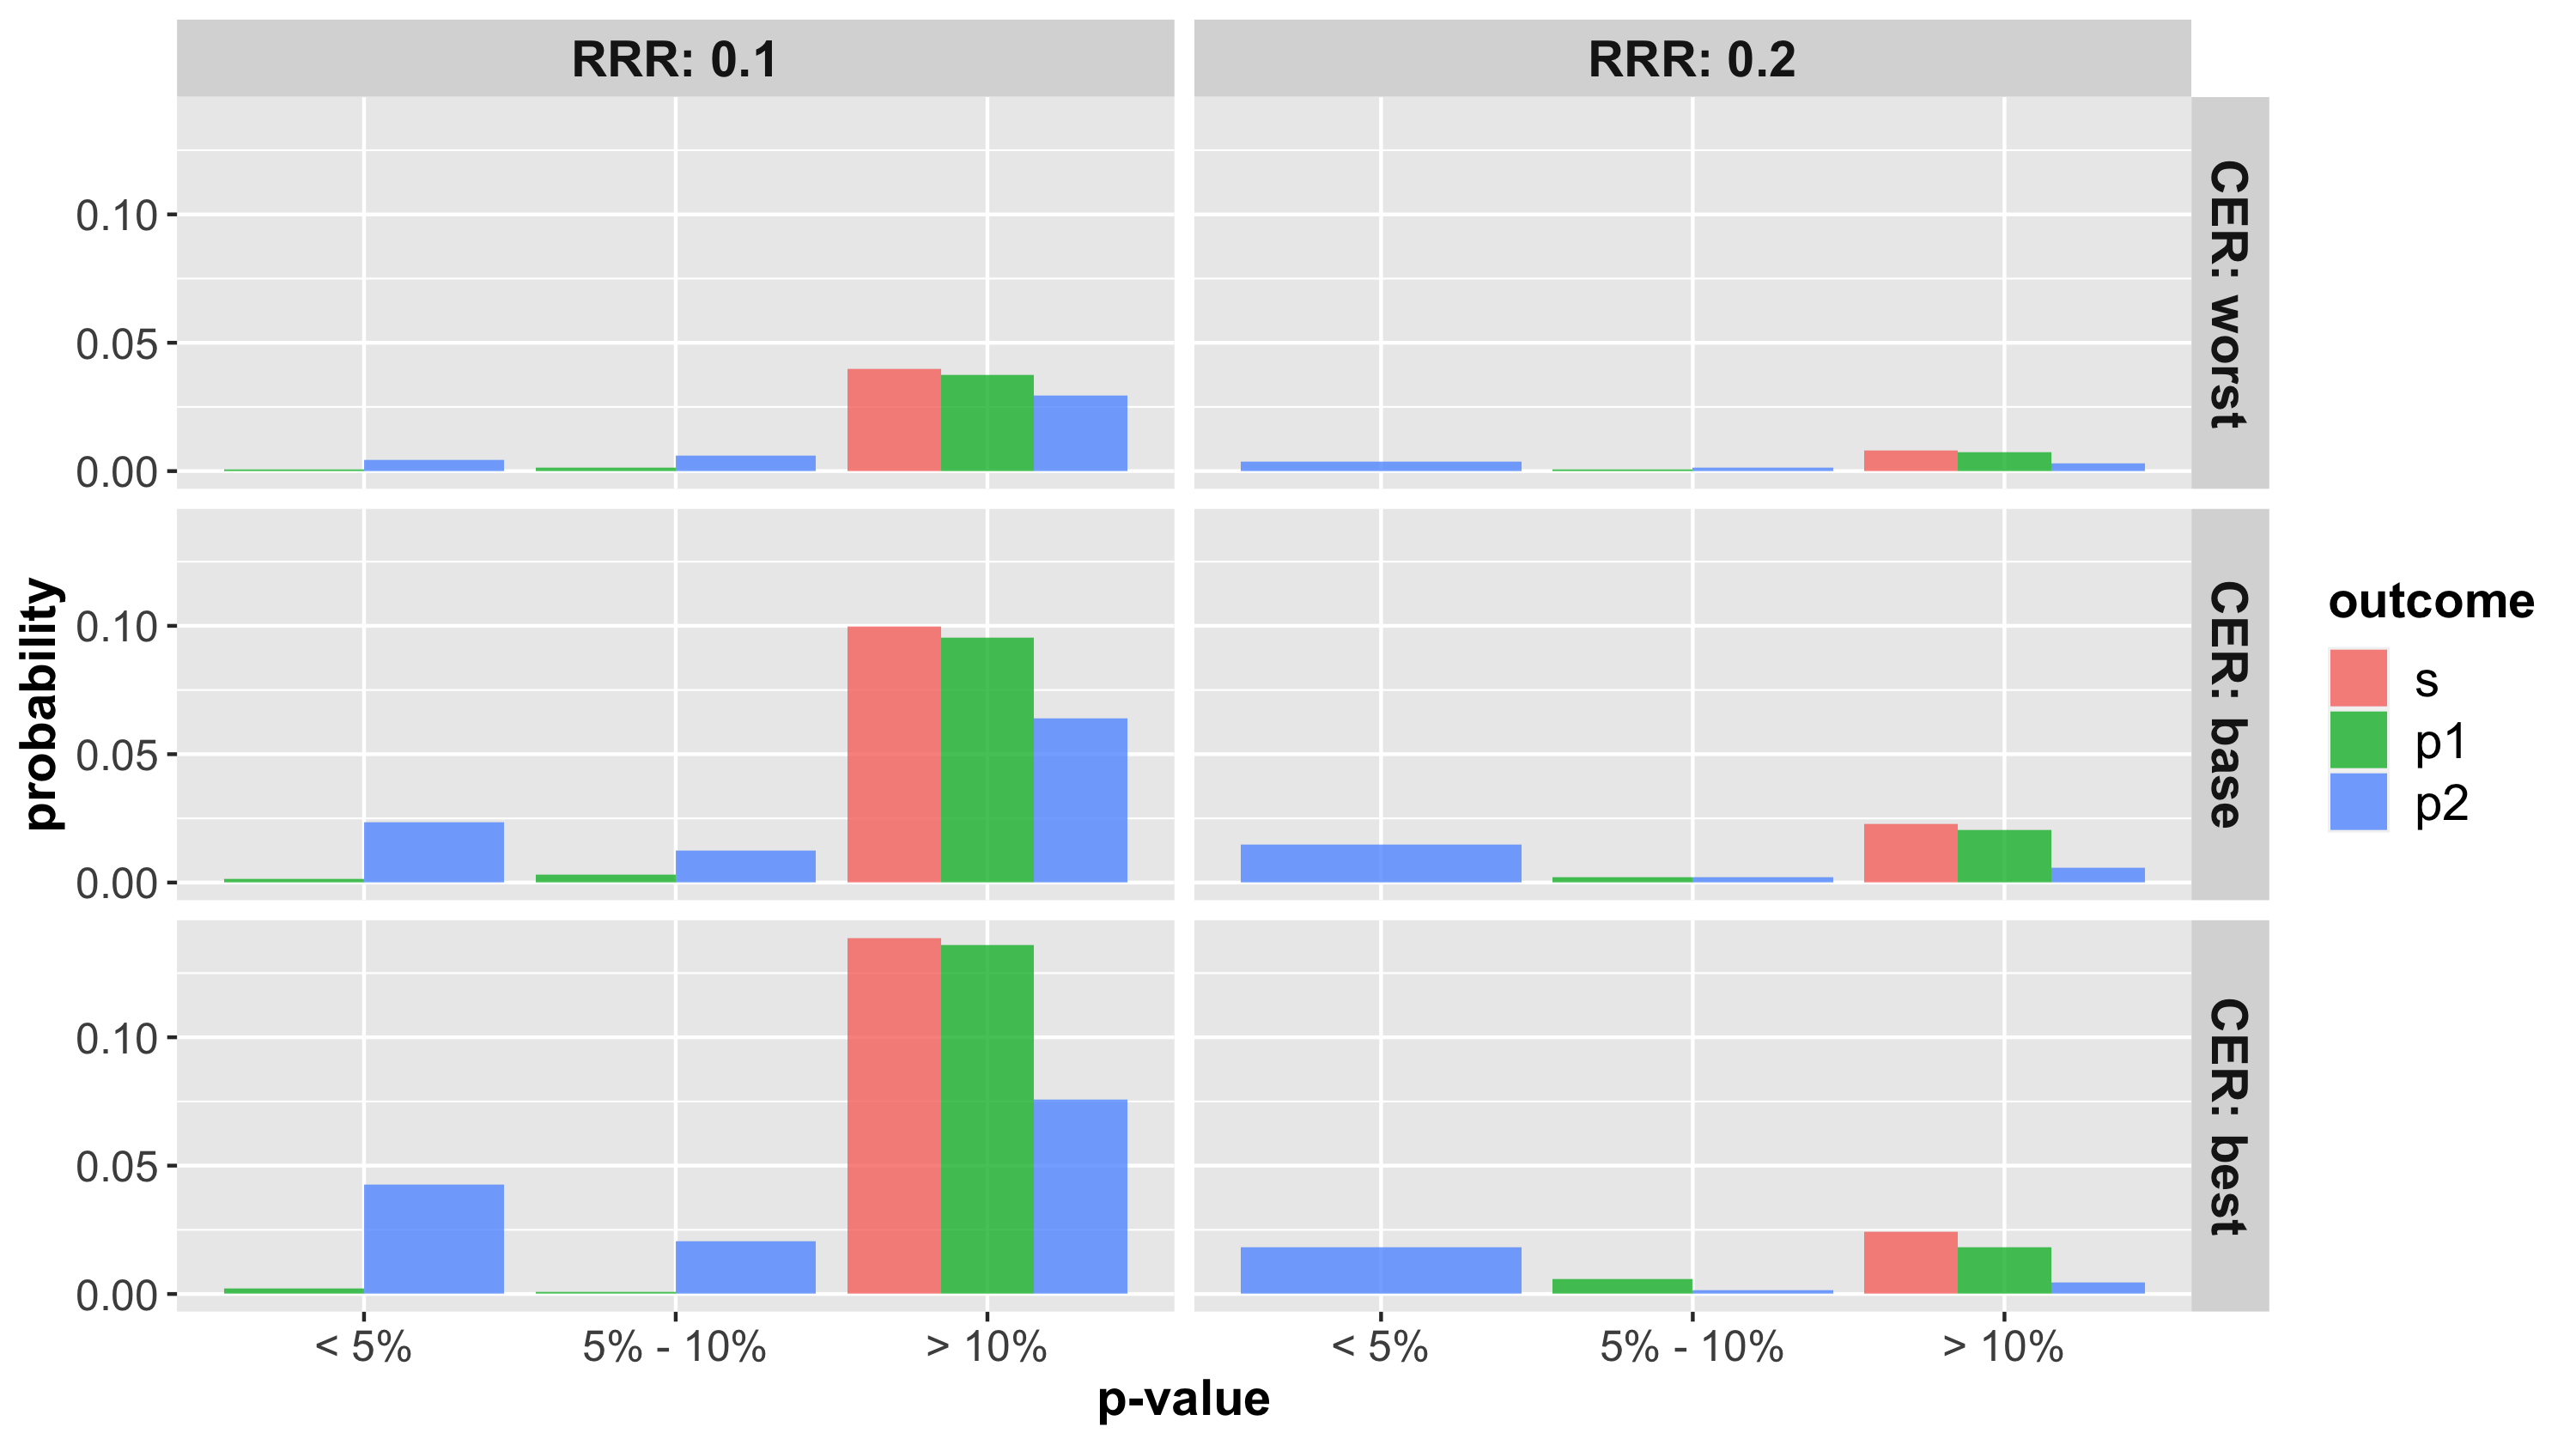
\includegraphics{../p1_plots/batch_size_nb_3000/pvalue_fut_p1.png}
  \end{subfigure}
  \bigbreak
  \begin{subfigure}{0.8\textwidth}
    \centering
    \caption{}
    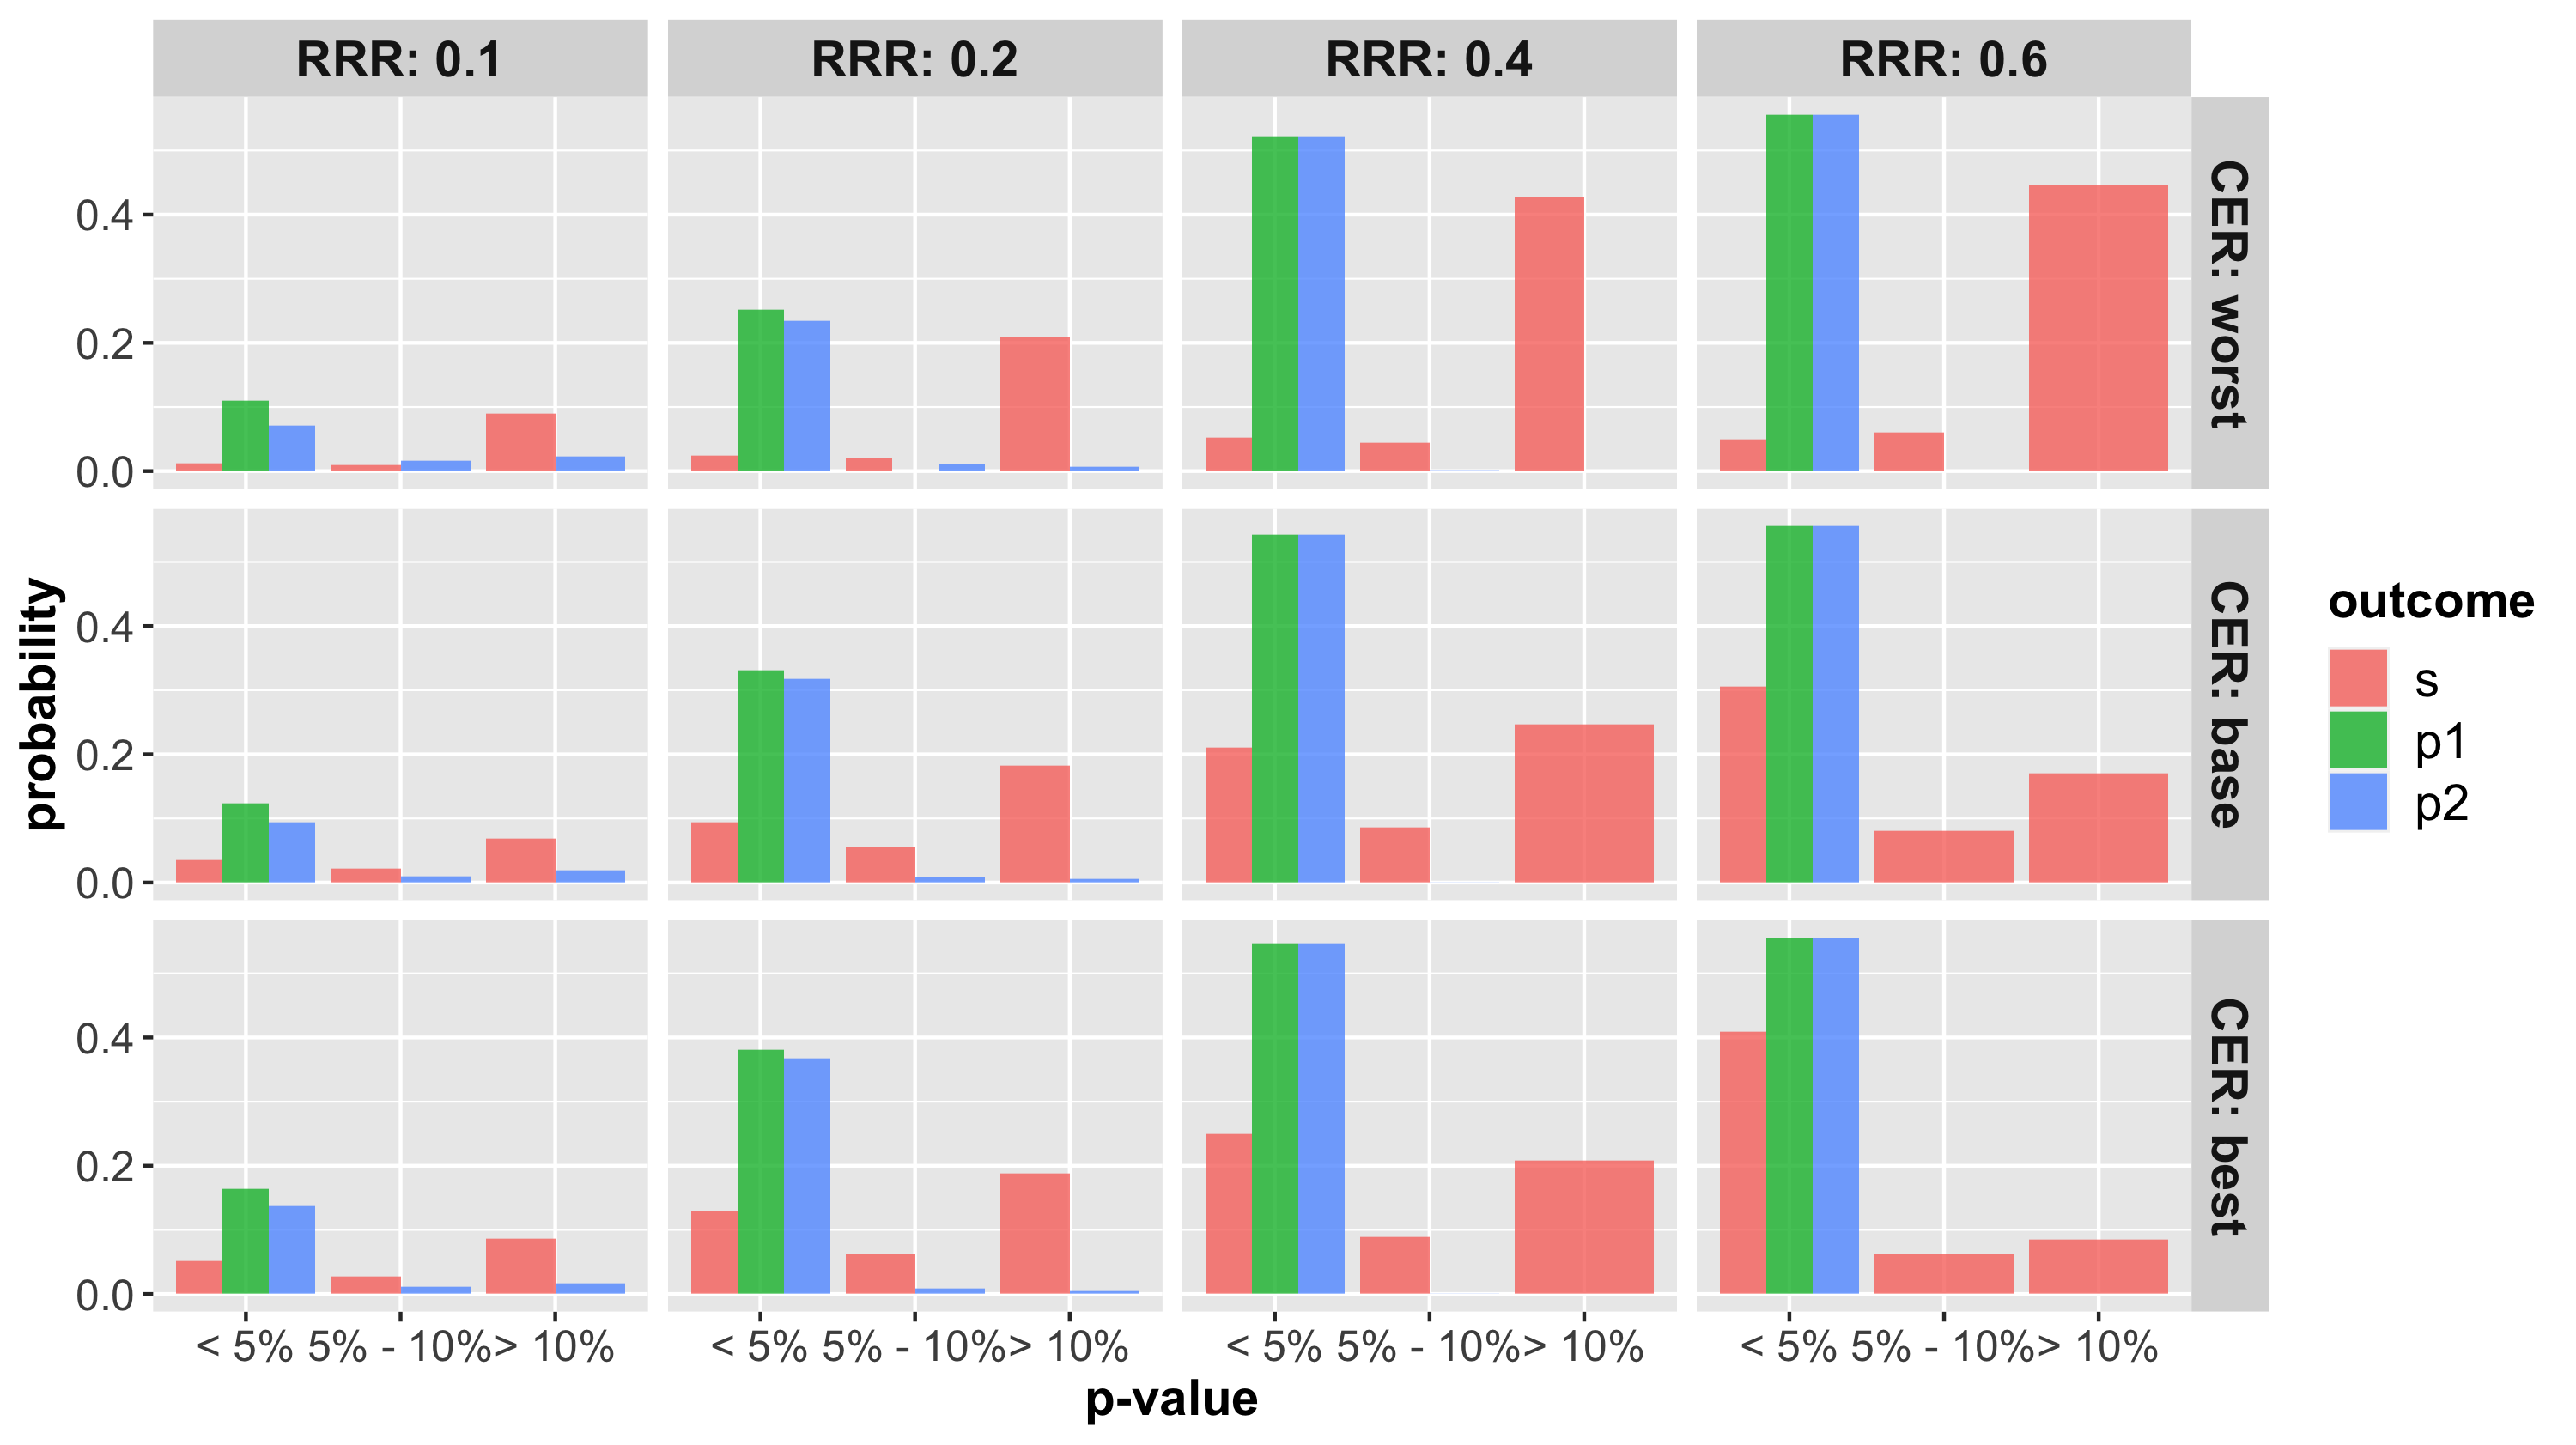
\includegraphics{../p1_plots/batch_size_nb_3000/pvalue_sup_p1.png}
  \end{subfigure}
\end{figure}

\hypertarget{relative-risk-reduction-estimates-at-trial-termination-2}{%
\paragraph{Relative risk reduction estimates at trial
termination}\label{relative-risk-reduction-estimates-at-trial-termination-2}}

\begin{figure}
  \caption{Distribution of relative risk reduction estimates (smoothed by a kernel density estimator) for the three
  control event rates (CER – rows), four relative risk reductions (RRR – columns) and the three outcomes (legend).}
  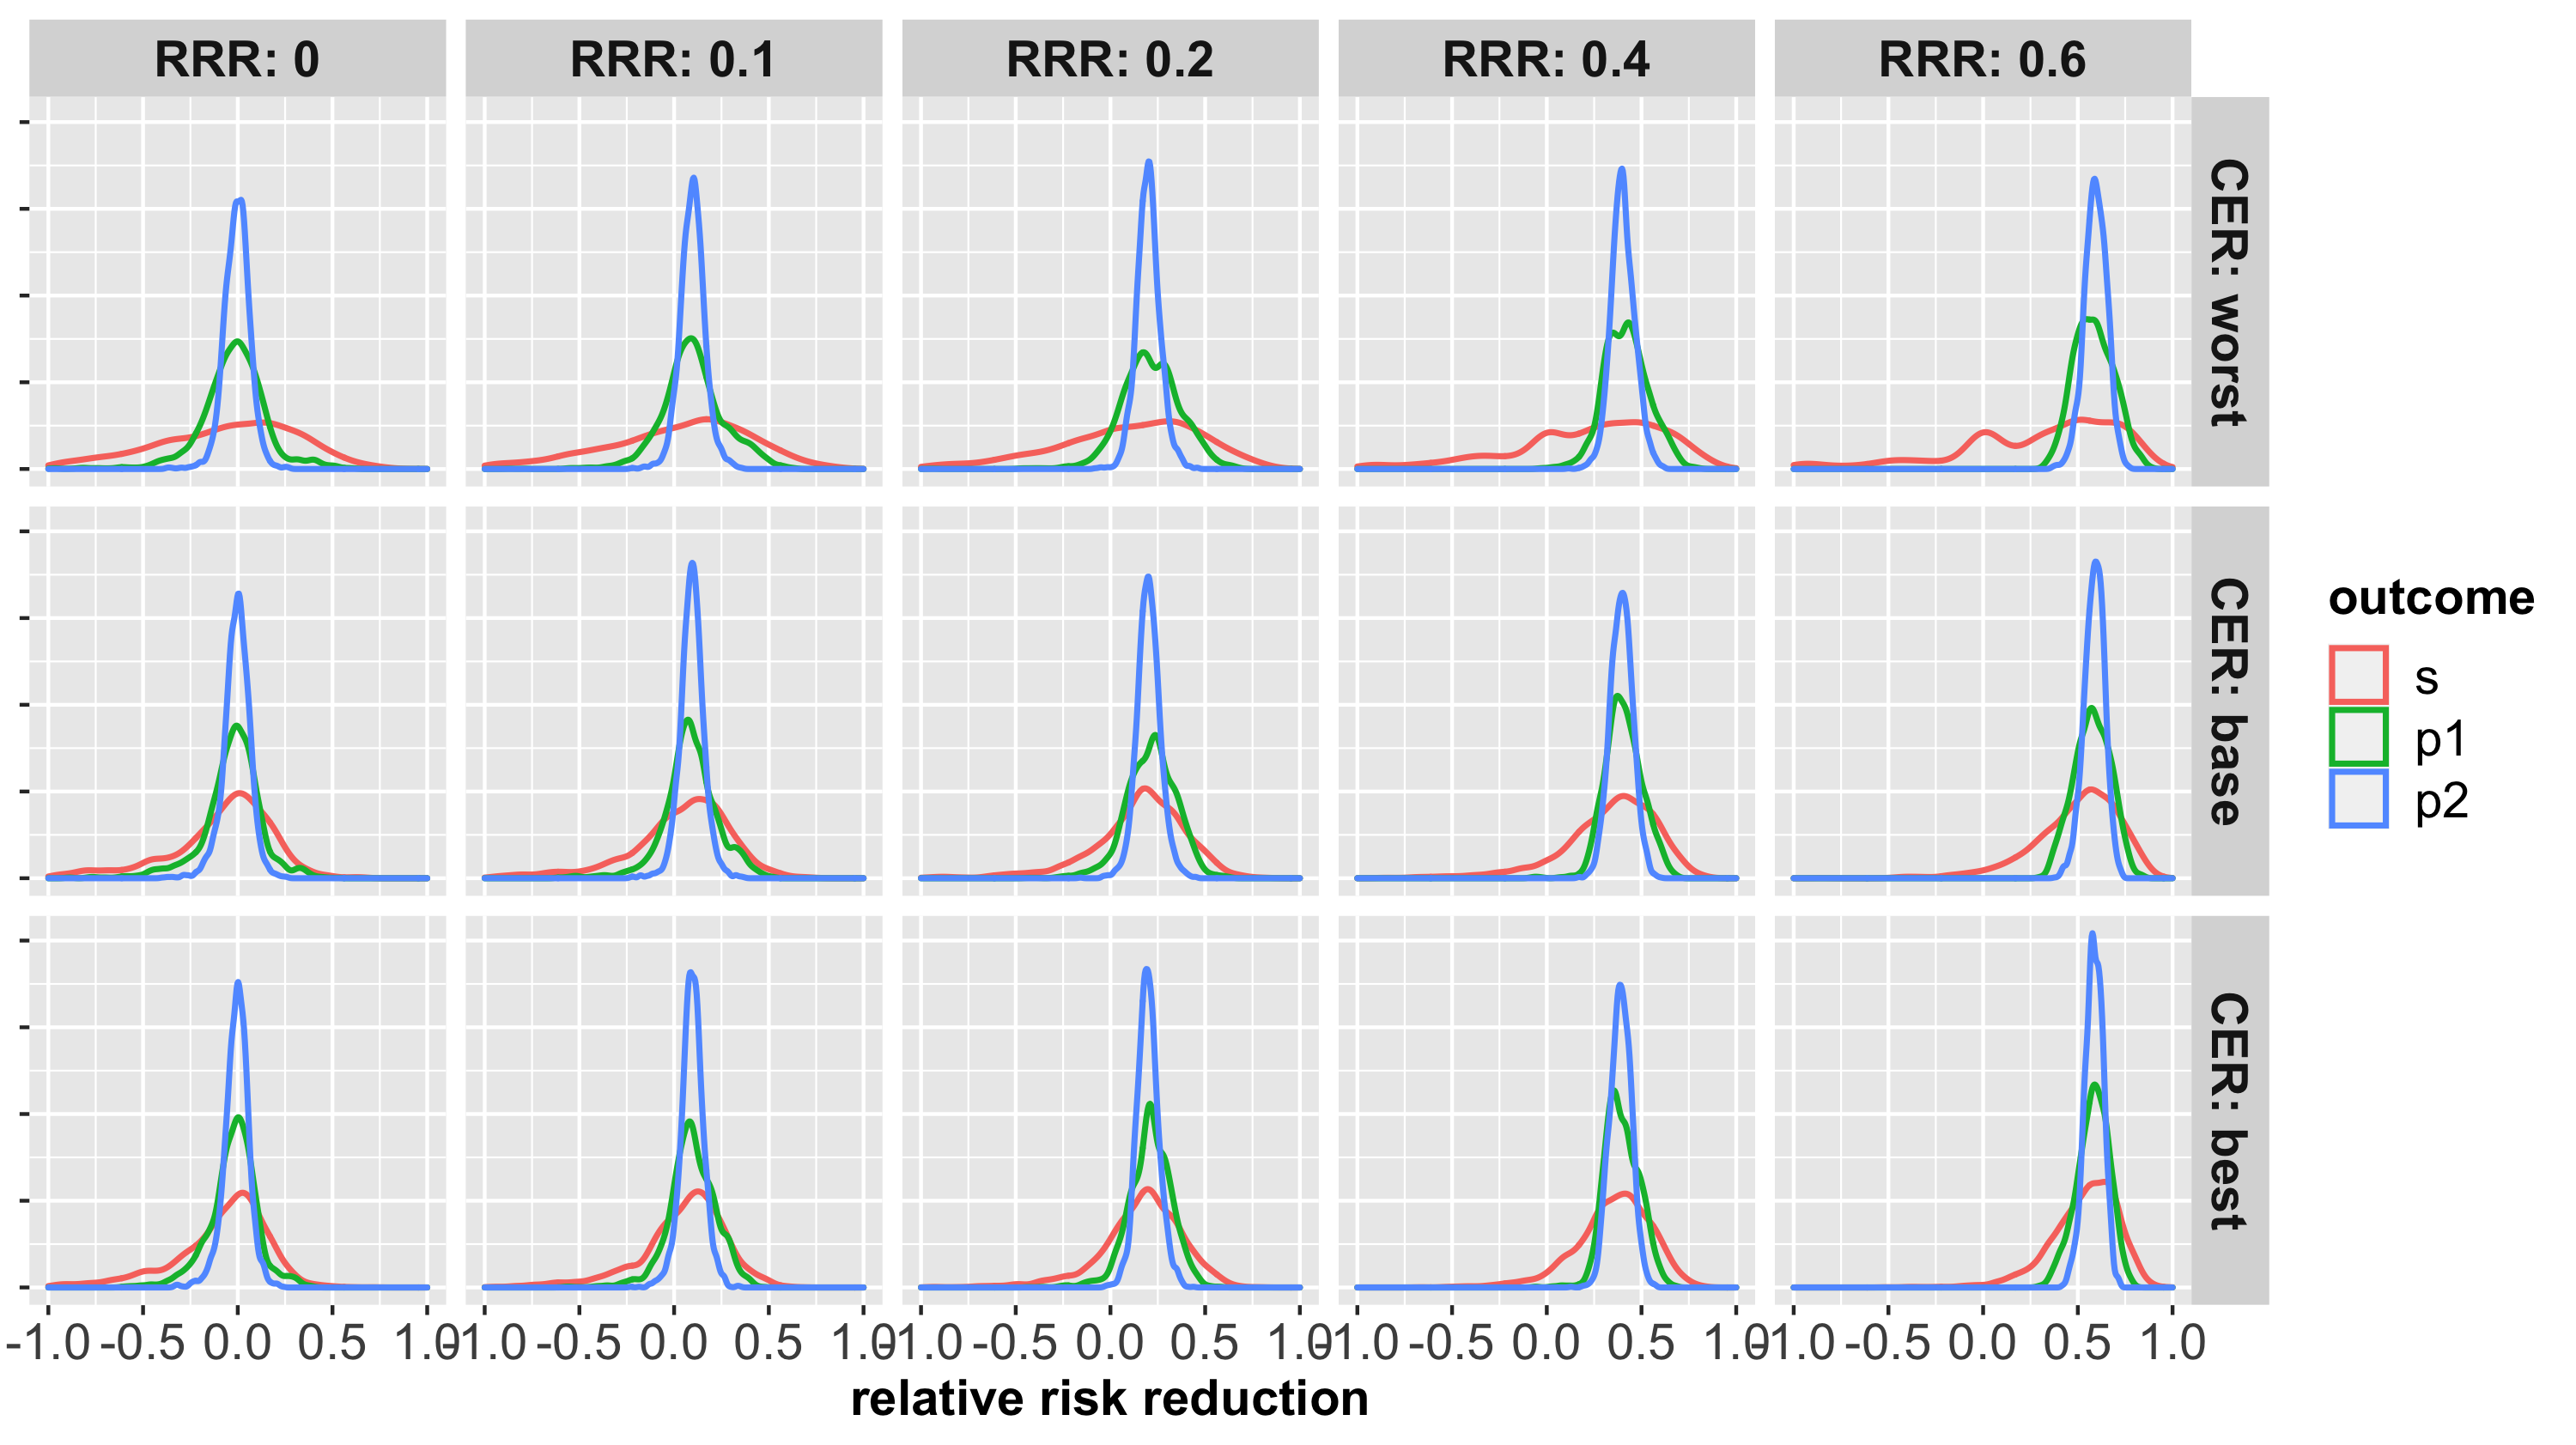
\includegraphics{../p1_plots/batch_size_nb_3000/RRRhat_p1.png}
\end{figure}

\begin{figure}
\centering
  \caption{Distribution of relative risk reduction estimates after stopping early for (a) futility; (b) superiority.
  Results are presented for the three control event rates by rows, four relative risk reductions (by columns) and the
  three outcomes (legend).}
  \begin{subfigure}{0.8\textwidth}
    \centering
    \caption{}
    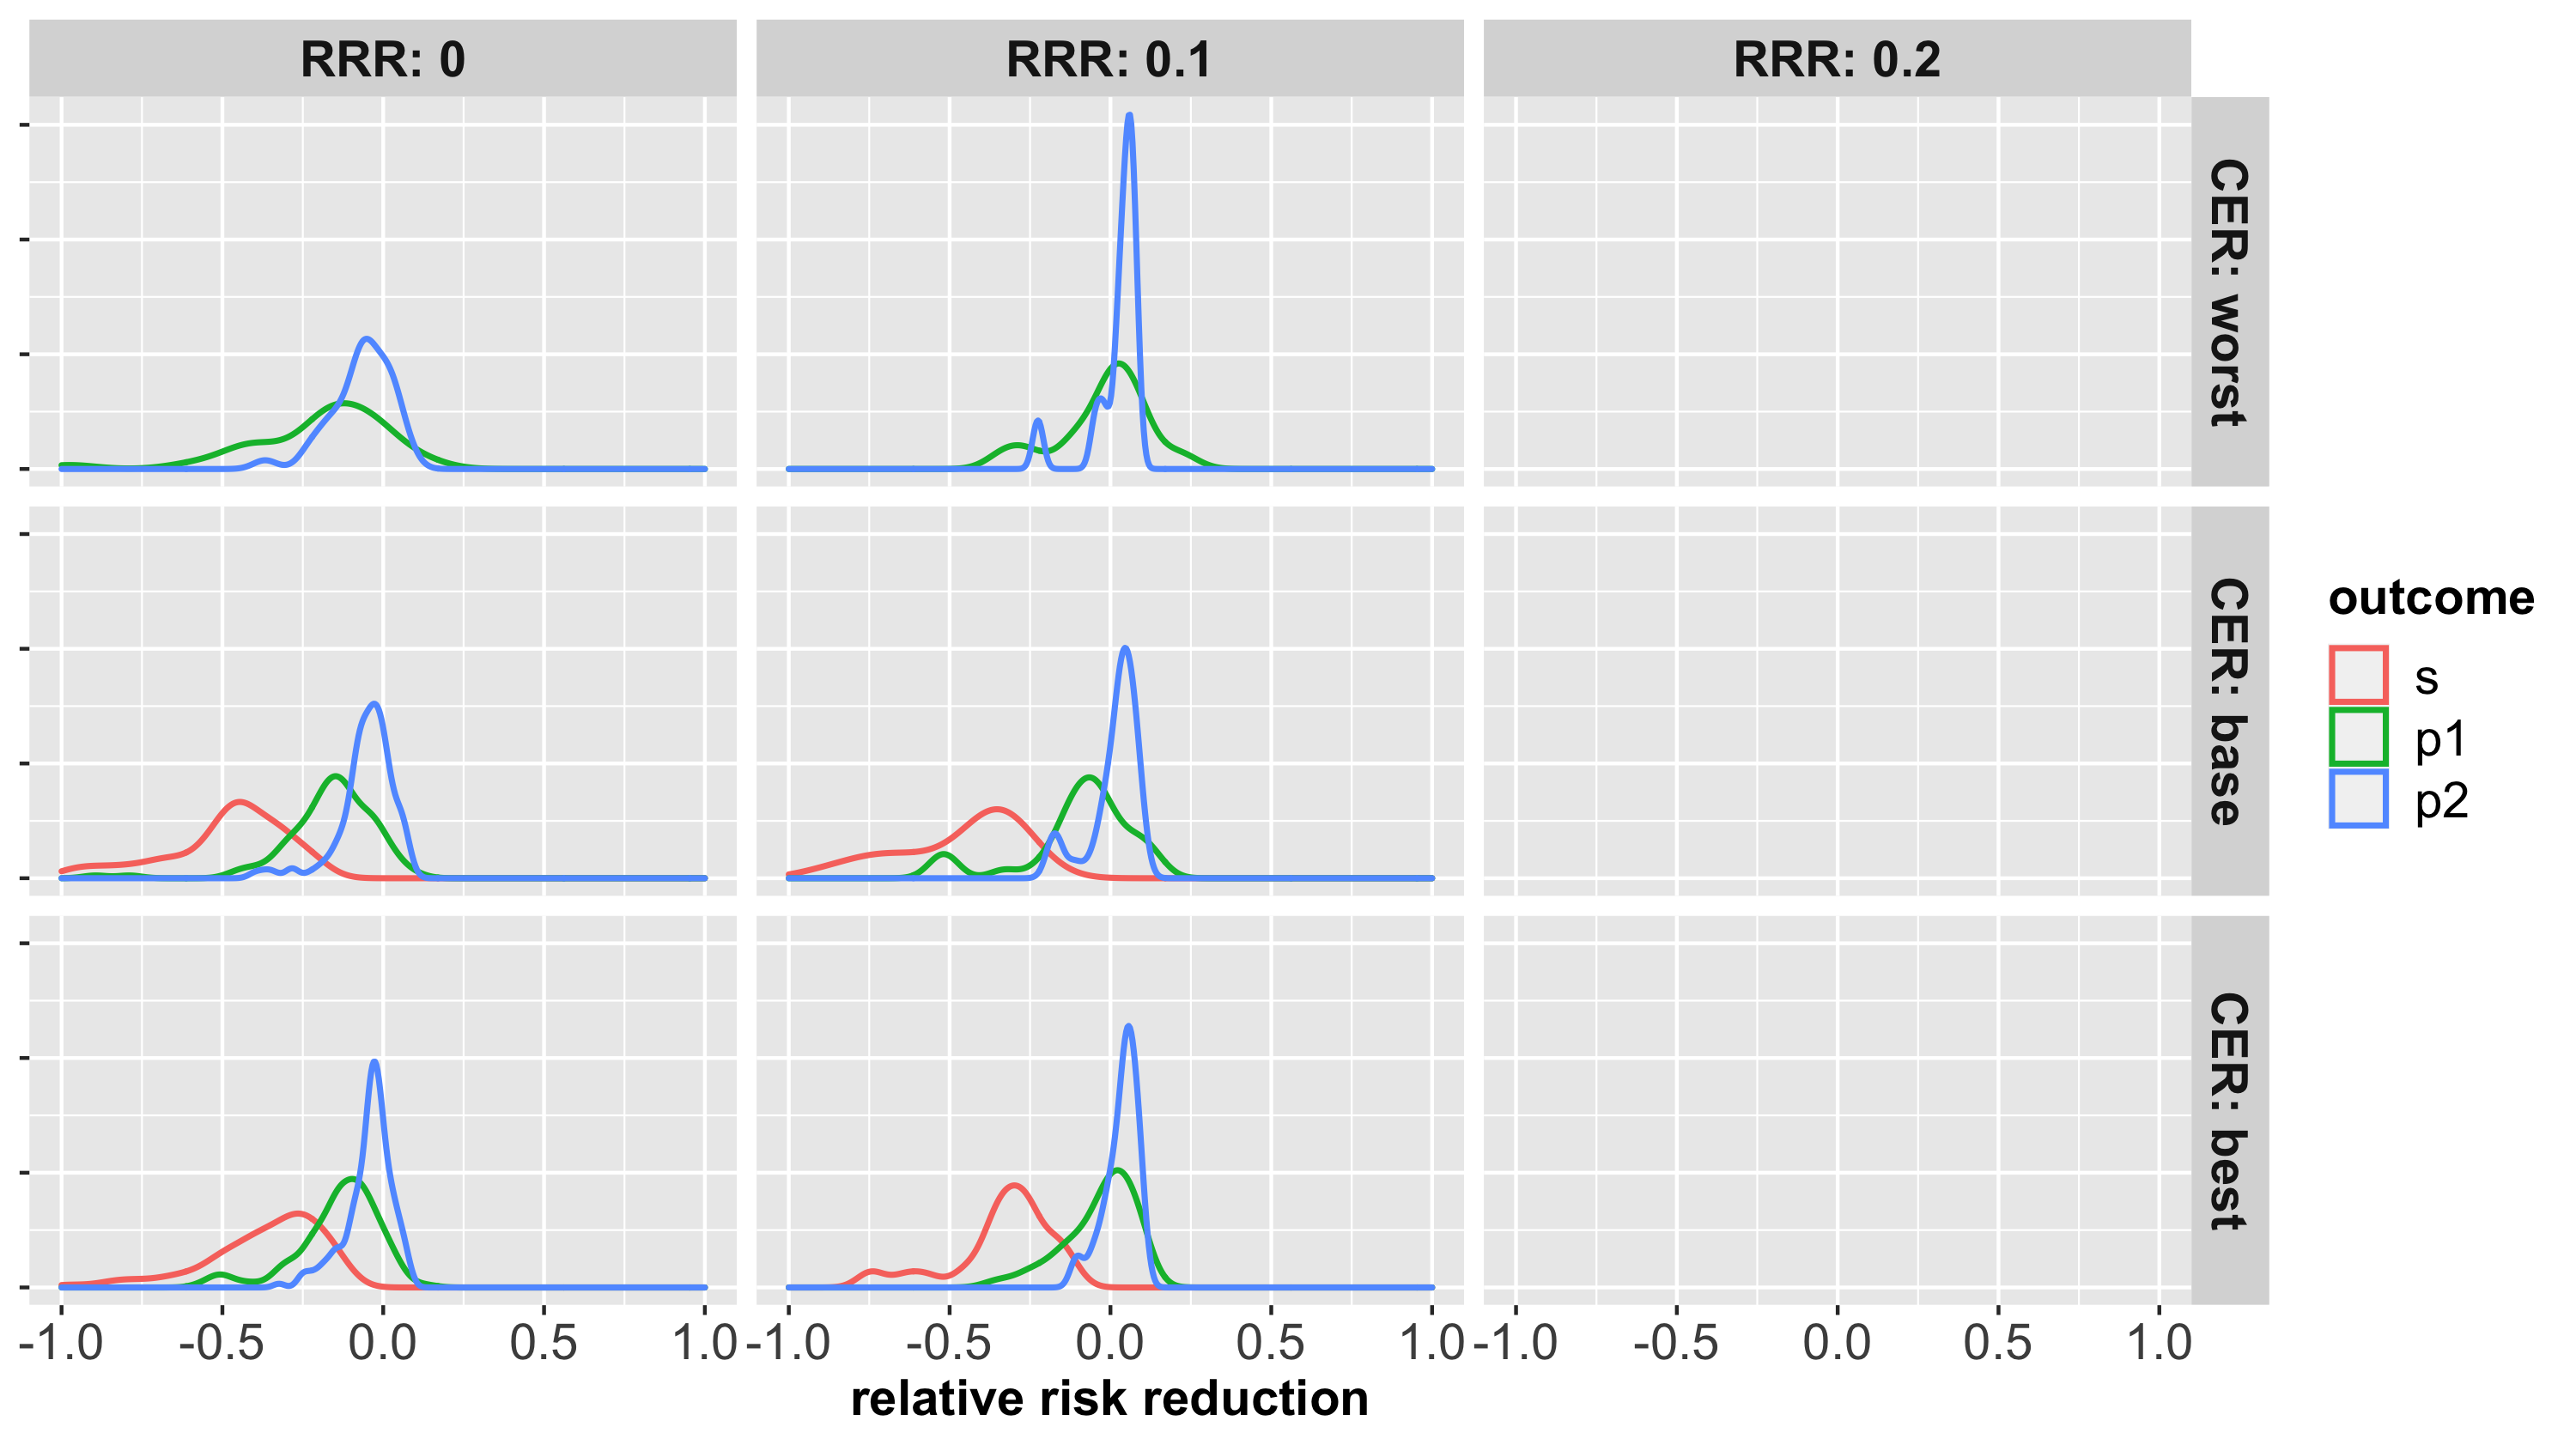
\includegraphics{../p1_plots/batch_size_nb_3000/RRRhat_fut_p1.png}
  \end{subfigure}
  \bigbreak
  \begin{subfigure}{0.8\textwidth}
    \centering
    \caption{}
    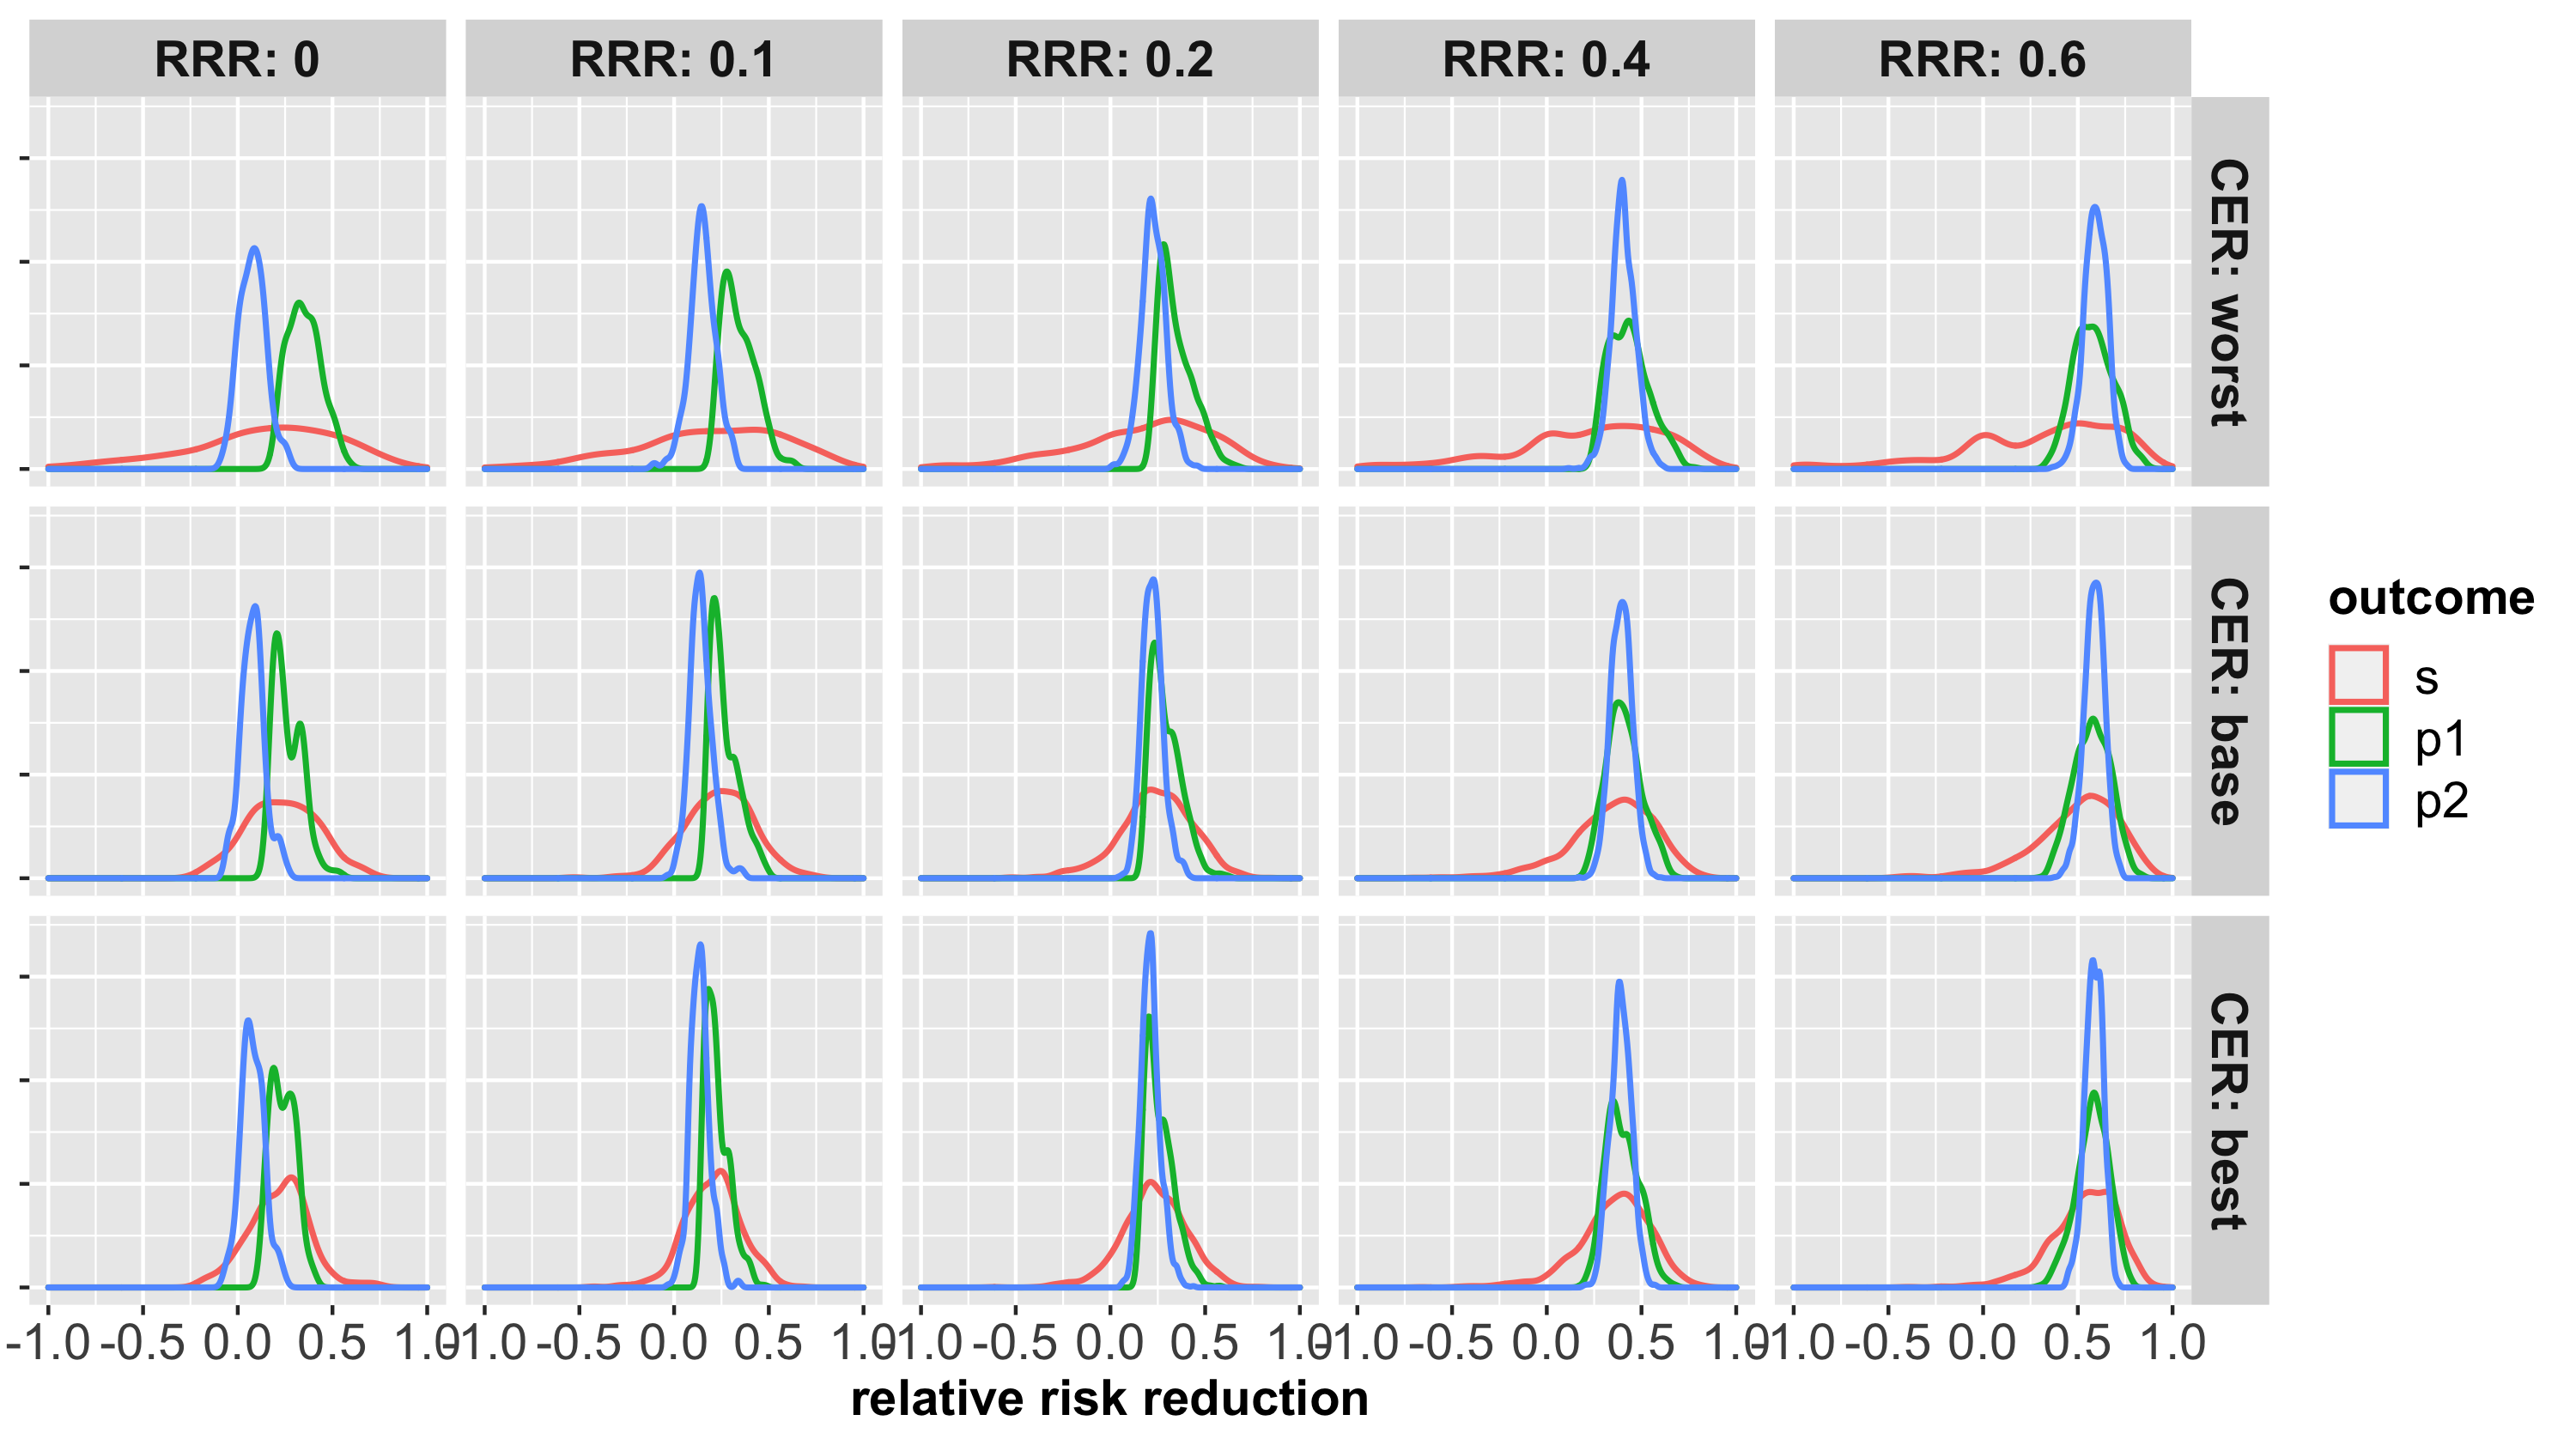
\includegraphics{../p1_plots/batch_size_nb_3000/RRRhat_sup_p1.png}
  \end{subfigure}
\end{figure}

\end{document}
